
\documentclass{article} % For LaTeX2e

\usepackage[table]{xcolor}
\usepackage{template/iclr2024_conference,times}

% Optional math commands from https://github.com/goodfeli/dlbook_notation.

\usepackage{amsmath,amsfonts,bm}

\newcommand{\figleft}{{\em (Left)}}
\newcommand{\figcenter}{{\em (Center)}}
\newcommand{\figright}{{\em (Right)}}
\newcommand{\figtop}{{\em (Top)}}
\newcommand{\figbottom}{{\em (Bottom)}}
\newcommand{\captiona}{{\em (a)}}
\newcommand{\captionb}{{\em (b)}}
\newcommand{\captionc}{{\em (c)}}
\newcommand{\captiond}{{\em (d)}}

\newcommand{\newterm}[1]{{\bf #1}}


\def\figref#1{figure~\ref{#1}}
\def\Figref#1{Figure~\ref{#1}}
\def\twofigref#1#2{figures \ref{#1} and \ref{#2}}
\def\quadfigref#1#2#3#4{figures \ref{#1}, \ref{#2}, \ref{#3} and \ref{#4}}
\def\secref#1{section~\ref{#1}}
\def\Secref#1{Section~\ref{#1}}
\def\twosecrefs#1#2{sections \ref{#1} and \ref{#2}}
\def\secrefs#1#2#3{sections \ref{#1}, \ref{#2} and \ref{#3}}
\def\eqref#1{equation~\ref{#1}}
\def\Eqref#1{Equation~\ref{#1}}
\def\plaineqref#1{\ref{#1}}
\def\chapref#1{chapter~\ref{#1}}
\def\Chapref#1{Chapter~\ref{#1}}
\def\rangechapref#1#2{chapters\ref{#1}--\ref{#2}}
\def\algref#1{algorithm~\ref{#1}}
\def\Algref#1{Algorithm~\ref{#1}}
\def\twoalgref#1#2{algorithms \ref{#1} and \ref{#2}}
\def\Twoalgref#1#2{Algorithms \ref{#1} and \ref{#2}}
\def\partref#1{part~\ref{#1}}
\def\Partref#1{Part~\ref{#1}}
\def\twopartref#1#2{parts \ref{#1} and \ref{#2}}

\def\ceil#1{\lceil #1 \rceil}
\def\floor#1{\lfloor #1 \rfloor}
\def\1{\bm{1}}
\newcommand{\train}{\mathcal{D}}
\newcommand{\valid}{\mathcal{D_{\mathrm{valid}}}}
\newcommand{\test}{\mathcal{D_{\mathrm{test}}}}

\def\eps{{\epsilon}}


\def\reta{{\textnormal{$\eta$}}}
\def\ra{{\textnormal{a}}}
\def\rb{{\textnormal{b}}}
\def\rc{{\textnormal{c}}}
\def\rd{{\textnormal{d}}}
\def\re{{\textnormal{e}}}
\def\rf{{\textnormal{f}}}
\def\rg{{\textnormal{g}}}
\def\rh{{\textnormal{h}}}
\def\ri{{\textnormal{i}}}
\def\rj{{\textnormal{j}}}
\def\rk{{\textnormal{k}}}
\def\rl{{\textnormal{l}}}
\def\rn{{\textnormal{n}}}
\def\ro{{\textnormal{o}}}
\def\rp{{\textnormal{p}}}
\def\rq{{\textnormal{q}}}
\def\rr{{\textnormal{r}}}
\def\rs{{\textnormal{s}}}
\def\rt{{\textnormal{t}}}
\def\ru{{\textnormal{u}}}
\def\rv{{\textnormal{v}}}
\def\rw{{\textnormal{w}}}
\def\rx{{\textnormal{x}}}
\def\ry{{\textnormal{y}}}
\def\rz{{\textnormal{z}}}

\def\rvepsilon{{\mathbf{\epsilon}}}
\def\rvtheta{{\mathbf{\theta}}}
\def\rva{{\mathbf{a}}}
\def\rvb{{\mathbf{b}}}
\def\rvc{{\mathbf{c}}}
\def\rvd{{\mathbf{d}}}
\def\rve{{\mathbf{e}}}
\def\rvf{{\mathbf{f}}}
\def\rvg{{\mathbf{g}}}
\def\rvh{{\mathbf{h}}}
\def\rvu{{\mathbf{i}}}
\def\rvj{{\mathbf{j}}}
\def\rvk{{\mathbf{k}}}
\def\rvl{{\mathbf{l}}}
\def\rvm{{\mathbf{m}}}
\def\rvn{{\mathbf{n}}}
\def\rvo{{\mathbf{o}}}
\def\rvp{{\mathbf{p}}}
\def\rvq{{\mathbf{q}}}
\def\rvr{{\mathbf{r}}}
\def\rvs{{\mathbf{s}}}
\def\rvt{{\mathbf{t}}}
\def\rvu{{\mathbf{u}}}
\def\rvv{{\mathbf{v}}}
\def\rvw{{\mathbf{w}}}
\def\rvx{{\mathbf{x}}}
\def\rvy{{\mathbf{y}}}
\def\rvz{{\mathbf{z}}}

\def\erva{{\textnormal{a}}}
\def\ervb{{\textnormal{b}}}
\def\ervc{{\textnormal{c}}}
\def\ervd{{\textnormal{d}}}
\def\erve{{\textnormal{e}}}
\def\ervf{{\textnormal{f}}}
\def\ervg{{\textnormal{g}}}
\def\ervh{{\textnormal{h}}}
\def\ervi{{\textnormal{i}}}
\def\ervj{{\textnormal{j}}}
\def\ervk{{\textnormal{k}}}
\def\ervl{{\textnormal{l}}}
\def\ervm{{\textnormal{m}}}
\def\ervn{{\textnormal{n}}}
\def\ervo{{\textnormal{o}}}
\def\ervp{{\textnormal{p}}}
\def\ervq{{\textnormal{q}}}
\def\ervr{{\textnormal{r}}}
\def\ervs{{\textnormal{s}}}
\def\ervt{{\textnormal{t}}}
\def\ervu{{\textnormal{u}}}
\def\ervv{{\textnormal{v}}}
\def\ervw{{\textnormal{w}}}
\def\ervx{{\textnormal{x}}}
\def\ervy{{\textnormal{y}}}
\def\ervz{{\textnormal{z}}}

\def\rmA{{\mathbf{A}}}
\def\rmB{{\mathbf{B}}}
\def\rmC{{\mathbf{C}}}
\def\rmD{{\mathbf{D}}}
\def\rmE{{\mathbf{E}}}
\def\rmF{{\mathbf{F}}}
\def\rmG{{\mathbf{G}}}
\def\rmH{{\mathbf{H}}}
\def\rmI{{\mathbf{I}}}
\def\rmJ{{\mathbf{J}}}
\def\rmK{{\mathbf{K}}}
\def\rmL{{\mathbf{L}}}
\def\rmM{{\mathbf{M}}}
\def\rmN{{\mathbf{N}}}
\def\rmO{{\mathbf{O}}}
\def\rmP{{\mathbf{P}}}
\def\rmQ{{\mathbf{Q}}}
\def\rmR{{\mathbf{R}}}
\def\rmS{{\mathbf{S}}}
\def\rmT{{\mathbf{T}}}
\def\rmU{{\mathbf{U}}}
\def\rmV{{\mathbf{V}}}
\def\rmW{{\mathbf{W}}}
\def\rmX{{\mathbf{X}}}
\def\rmY{{\mathbf{Y}}}
\def\rmZ{{\mathbf{Z}}}

\def\ermA{{\textnormal{A}}}
\def\ermB{{\textnormal{B}}}
\def\ermC{{\textnormal{C}}}
\def\ermD{{\textnormal{D}}}
\def\ermE{{\textnormal{E}}}
\def\ermF{{\textnormal{F}}}
\def\ermG{{\textnormal{G}}}
\def\ermH{{\textnormal{H}}}
\def\ermI{{\textnormal{I}}}
\def\ermJ{{\textnormal{J}}}
\def\ermK{{\textnormal{K}}}
\def\ermL{{\textnormal{L}}}
\def\ermM{{\textnormal{M}}}
\def\ermN{{\textnormal{N}}}
\def\ermO{{\textnormal{O}}}
\def\ermP{{\textnormal{P}}}
\def\ermQ{{\textnormal{Q}}}
\def\ermR{{\textnormal{R}}}
\def\ermS{{\textnormal{S}}}
\def\ermT{{\textnormal{T}}}
\def\ermU{{\textnormal{U}}}
\def\ermV{{\textnormal{V}}}
\def\ermW{{\textnormal{W}}}
\def\ermX{{\textnormal{X}}}
\def\ermY{{\textnormal{Y}}}
\def\ermZ{{\textnormal{Z}}}

\def\vzero{{\bm{0}}}
\def\vone{{\bm{1}}}
\def\vmu{{\bm{\mu}}}
\def\vtheta{{\bm{\theta}}}
\def\va{{\bm{a}}}
\def\vb{{\bm{b}}}
\def\vc{{\bm{c}}}
\def\vd{{\bm{d}}}
\def\ve{{\bm{e}}}
\def\vf{{\bm{f}}}
\def\vg{{\bm{g}}}
\def\vh{{\bm{h}}}
\def\vi{{\bm{i}}}
\def\vj{{\bm{j}}}
\def\vk{{\bm{k}}}
\def\vl{{\bm{l}}}
\def\vm{{\bm{m}}}
\def\vn{{\bm{n}}}
\def\vo{{\bm{o}}}
\def\vp{{\bm{p}}}
\def\vq{{\bm{q}}}
\def\vr{{\bm{r}}}
\def\vs{{\bm{s}}}
\def\vt{{\bm{t}}}
\def\vu{{\bm{u}}}
\def\vv{{\bm{v}}}
\def\vw{{\bm{w}}}
\def\vx{{\bm{x}}}
\def\vy{{\bm{y}}}
\def\vz{{\bm{z}}}

\def\evalpha{{\alpha}}
\def\evbeta{{\beta}}
\def\evepsilon{{\epsilon}}
\def\evlambda{{\lambda}}
\def\evomega{{\omega}}
\def\evmu{{\mu}}
\def\evpsi{{\psi}}
\def\evsigma{{\sigma}}
\def\evtheta{{\theta}}
\def\eva{{a}}
\def\evb{{b}}
\def\evc{{c}}
\def\evd{{d}}
\def\eve{{e}}
\def\evf{{f}}
\def\evg{{g}}
\def\evh{{h}}
\def\evi{{i}}
\def\evj{{j}}
\def\evk{{k}}
\def\evl{{l}}
\def\evm{{m}}
\def\evn{{n}}
\def\evo{{o}}
\def\evp{{p}}
\def\evq{{q}}
\def\evr{{r}}
\def\evs{{s}}
\def\evt{{t}}
\def\evu{{u}}
\def\evv{{v}}
\def\evw{{w}}
\def\evx{{x}}
\def\evy{{y}}
\def\evz{{z}}

\def\mA{{\bm{A}}}
\def\mB{{\bm{B}}}
\def\mC{{\bm{C}}}
\def\mD{{\bm{D}}}
\def\mE{{\bm{E}}}
\def\mF{{\bm{F}}}
\def\mG{{\bm{G}}}
\def\mH{{\bm{H}}}
\def\mI{{\bm{I}}}
\def\mJ{{\bm{J}}}
\def\mK{{\bm{K}}}
\def\mL{{\bm{L}}}
\def\mM{{\bm{M}}}
\def\mN{{\bm{N}}}
\def\mO{{\bm{O}}}
\def\mP{{\bm{P}}}
\def\mQ{{\bm{Q}}}
\def\mR{{\bm{R}}}
\def\mS{{\bm{S}}}
\def\mT{{\bm{T}}}
\def\mU{{\bm{U}}}
\def\mV{{\bm{V}}}
\def\mW{{\bm{W}}}
\def\mX{{\bm{X}}}
\def\mY{{\bm{Y}}}
\def\mZ{{\bm{Z}}}
\def\mBeta{{\bm{\beta}}}
\def\mPhi{{\bm{\Phi}}}
\def\mLambda{{\bm{\Lambda}}}
\def\mSigma{{\bm{\Sigma}}}

\DeclareMathAlphabet{\mathsfit}{\encodingdefault}{\sfdefault}{m}{sl}
\SetMathAlphabet{\mathsfit}{bold}{\encodingdefault}{\sfdefault}{bx}{n}
\newcommand{\tens}[1]{\bm{\mathsfit{#1}}}
\def\tA{{\tens{A}}}
\def\tB{{\tens{B}}}
\def\tC{{\tens{C}}}
\def\tD{{\tens{D}}}
\def\tE{{\tens{E}}}
\def\tF{{\tens{F}}}
\def\tG{{\tens{G}}}
\def\tH{{\tens{H}}}
\def\tI{{\tens{I}}}
\def\tJ{{\tens{J}}}
\def\tK{{\tens{K}}}
\def\tL{{\tens{L}}}
\def\tM{{\tens{M}}}
\def\tN{{\tens{N}}}
\def\tO{{\tens{O}}}
\def\tP{{\tens{P}}}
\def\tQ{{\tens{Q}}}
\def\tR{{\tens{R}}}
\def\tS{{\tens{S}}}
\def\tT{{\tens{T}}}
\def\tU{{\tens{U}}}
\def\tV{{\tens{V}}}
\def\tW{{\tens{W}}}
\def\tX{{\tens{X}}}
\def\tY{{\tens{Y}}}
\def\tZ{{\tens{Z}}}


\def\gA{{\mathcal{A}}}
\def\gB{{\mathcal{B}}}
\def\gC{{\mathcal{C}}}
\def\gD{{\mathcal{D}}}
\def\gE{{\mathcal{E}}}
\def\gF{{\mathcal{F}}}
\def\gG{{\mathcal{G}}}
\def\gH{{\mathcal{H}}}
\def\gI{{\mathcal{I}}}
\def\gJ{{\mathcal{J}}}
\def\gK{{\mathcal{K}}}
\def\gL{{\mathcal{L}}}
\def\gM{{\mathcal{M}}}
\def\gN{{\mathcal{N}}}
\def\gO{{\mathcal{O}}}
\def\gP{{\mathcal{P}}}
\def\gQ{{\mathcal{Q}}}
\def\gR{{\mathcal{R}}}
\def\gS{{\mathcal{S}}}
\def\gT{{\mathcal{T}}}
\def\gU{{\mathcal{U}}}
\def\gV{{\mathcal{V}}}
\def\gW{{\mathcal{W}}}
\def\gX{{\mathcal{X}}}
\def\gY{{\mathcal{Y}}}
\def\gZ{{\mathcal{Z}}}

\def\sA{{\mathbb{A}}}
\def\sB{{\mathbb{B}}}
\def\sC{{\mathbb{C}}}
\def\sD{{\mathbb{D}}}
\def\sF{{\mathbb{F}}}
\def\sG{{\mathbb{G}}}
\def\sH{{\mathbb{H}}}
\def\sI{{\mathbb{I}}}
\def\sJ{{\mathbb{J}}}
\def\sK{{\mathbb{K}}}
\def\sL{{\mathbb{L}}}
\def\sM{{\mathbb{M}}}
\def\sN{{\mathbb{N}}}
\def\sO{{\mathbb{O}}}
\def\sP{{\mathbb{P}}}
\def\sQ{{\mathbb{Q}}}
\def\sR{{\mathbb{R}}}
\def\sS{{\mathbb{S}}}
\def\sT{{\mathbb{T}}}
\def\sU{{\mathbb{U}}}
\def\sV{{\mathbb{V}}}
\def\sW{{\mathbb{W}}}
\def\sX{{\mathbb{X}}}
\def\sY{{\mathbb{Y}}}
\def\sZ{{\mathbb{Z}}}

\def\emLambda{{\Lambda}}
\def\emA{{A}}
\def\emB{{B}}
\def\emC{{C}}
\def\emD{{D}}
\def\emE{{E}}
\def\emF{{F}}
\def\emG{{G}}
\def\emH{{H}}
\def\emI{{I}}
\def\emJ{{J}}
\def\emK{{K}}
\def\emL{{L}}
\def\emM{{M}}
\def\emN{{N}}
\def\emO{{O}}
\def\emP{{P}}
\def\emQ{{Q}}
\def\emR{{R}}
\def\emS{{S}}
\def\emT{{T}}
\def\emU{{U}}
\def\emV{{V}}
\def\emW{{W}}
\def\emX{{X}}
\def\emY{{Y}}
\def\emZ{{Z}}
\def\emSigma{{\Sigma}}

\newcommand{\etens}[1]{\mathsfit{#1}}
\def\etLambda{{\etens{\Lambda}}}
\def\etA{{\etens{A}}}
\def\etB{{\etens{B}}}
\def\etC{{\etens{C}}}
\def\etD{{\etens{D}}}
\def\etE{{\etens{E}}}
\def\etF{{\etens{F}}}
\def\etG{{\etens{G}}}
\def\etH{{\etens{H}}}
\def\etI{{\etens{I}}}
\def\etJ{{\etens{J}}}
\def\etK{{\etens{K}}}
\def\etL{{\etens{L}}}
\def\etM{{\etens{M}}}
\def\etN{{\etens{N}}}
\def\etO{{\etens{O}}}
\def\etP{{\etens{P}}}
\def\etQ{{\etens{Q}}}
\def\etR{{\etens{R}}}
\def\etS{{\etens{S}}}
\def\etT{{\etens{T}}}
\def\etU{{\etens{U}}}
\def\etV{{\etens{V}}}
\def\etW{{\etens{W}}}
\def\etX{{\etens{X}}}
\def\etY{{\etens{Y}}}
\def\etZ{{\etens{Z}}}

\newcommand{\pdata}{p_{\rm{data}}}
\newcommand{\ptrain}{\hat{p}_{\rm{data}}}
\newcommand{\Ptrain}{\hat{P}_{\rm{data}}}
\newcommand{\pmodel}{p_{\rm{model}}}
\newcommand{\Pmodel}{P_{\rm{model}}}
\newcommand{\ptildemodel}{\tilde{p}_{\rm{model}}}
\newcommand{\pencode}{p_{\rm{encoder}}}
\newcommand{\pdecode}{p_{\rm{decoder}}}
\newcommand{\precons}{p_{\rm{reconstruct}}}

\newcommand{\laplace}{\mathrm{Laplace}} %

\newcommand{\E}{\mathbb{E}}
\newcommand{\Ls}{\mathcal{L}}
\newcommand{\R}{\mathbb{R}}
\newcommand{\emp}{\tilde{p}}
\newcommand{\lr}{\alpha}
\newcommand{\reg}{\lambda}
\newcommand{\rect}{\mathrm{rectifier}}
\newcommand{\softmax}{\mathrm{softmax}}
\newcommand{\sigmoid}{\sigma}
\newcommand{\softplus}{\zeta}
\newcommand{\KL}{D_{\mathrm{KL}}}
\newcommand{\Var}{\mathrm{Var}}
\newcommand{\standarderror}{\mathrm{SE}}
\newcommand{\Cov}{\mathrm{Cov}}
\newcommand{\normlzero}{L^0}
\newcommand{\normlone}{L^1}
\newcommand{\normltwo}{L^2}
\newcommand{\normlp}{L^p}
\newcommand{\normmax}{L^\infty}

\newcommand{\parents}{Pa} %

\DeclareMathOperator*{\argmax}{arg\,max}
\DeclareMathOperator*{\argmin}{arg\,min}

\DeclareMathOperator{\sign}{sign}
\DeclareMathOperator{\Tr}{Tr}
\let\ab\allowbreak


\definecolor{citecolor}{HTML}{0071BC}
\definecolor{linkcolor}{HTML}{ED1C24}

\usepackage[pagebackref=false, breaklinks=true, letterpaper=true, colorlinks, citecolor=citecolor, linkcolor=linkcolor, bookmarks=false]{hyperref}
\usepackage{url}
\usepackage{graphicx, mathtools, amsmath, amssymb, subcaption, multirow, overpic, textpos, pifont, xfrac, bbm}
\usepackage{microtype}
\usepackage[skip=4pt]{caption}
\usepackage{pythonhighlight}
\usepackage{listings}
\usepackage{inconsolata}
\usepackage{epsfig}
\usepackage{booktabs}
\usepackage[scaled=0.8]{FiraMono}
\usepackage[normalem]{ulem}
\usepackage{wrapfig}
\usepackage{adjustbox}
\usepackage{twemojis}

\def\name{ZipIt!}
\def\httilde{\mbox{\tt\raisebox{-.5ex}{\symbol{126}}}}

% \definecolor{zipcolor}{HTML}{EA4335}
% \definecolor{wavg}{HTML}{4285F4}
% \definecolor{gitrebasin}{HTML}{46BDC6}
% \newcommand*\zipcolor{\color{zipcolor}}
% \newcommand*\wavg{\color{wavg}}
% \newcommand*\gitrebasin{\color{gitrebasin}}

\makeatletter
\newcommand{\printfnsymbol}[1]{%
  \textsuperscript{\@fnsymbol{#1}}%
}
\makeatother

\newlength\savewidth\newcommand\shline{\noalign{\global\savewidth\arrayrulewidth
  \global\arrayrulewidth 0.75pt}\hline\noalign{\global\arrayrulewidth\savewidth}}
\newcommand{\tablestyle}[2]{\setlength{\tabcolsep}{#1}\renewcommand{\arraystretch}{#2}\centering\footnotesize}
\renewcommand{\paragraph}[1]{\vspace{1.25mm}\noindent\textbf{#1}}
\newcommand\blfootnote[1]{\begingroup\renewcommand\thefootnote{}\footnote{#1}\addtocounter{footnote}{-1}\endgroup}

\newcolumntype{x}[1]{>{\centering\arraybackslash}p{#1pt}}
\newcolumntype{y}[1]{>{\raggedright\arraybackslash}p{#1pt}}
\newcolumntype{z}[1]{>{\raggedleft\arraybackslash}p{#1pt}}

\newcommand{\app}{\raise.17ex\hbox{$\scriptstyle\sim$}}
\newcommand{\mypm}[1]{\color{gray}{\tiny{$\pm$#1}}}
\newcommand{\x}{{\times}}
\definecolor{deemph}{gray}{0.6}
\newcommand{\gc}[1]{\textcolor{deemph}{#1}}
\definecolor{defaultcolor}{gray}{.9}
\newcommand{\default}[1]{\cellcolor{defaultcolor}{#1}}
\newcommand{\authorskip}{\hspace{2.5mm}}

\definecolor{dt}{HTML}{ADCAD8}
\definecolor{dt2}{HTML}{cddfe7}
\newcommand{\ots}[1]{\textcolor{dt}{#1}}
\newcommand{\otsmodel}[1]{\cellcolor{dt2}{#1}}

\definecolor{modelacolor}{HTML}{85200c}
\definecolor{modelbcolor}{HTML}{0b5394}
\definecolor{modelccolor}{HTML}{351c75}
\definecolor{modeldcolor}{HTML}{664d00}

\newcommand{\modela}{\textcolor{modelacolor}}
\newcommand{\modelb}{\textcolor{modelbcolor}}
\newcommand{\modelc}{\textcolor{modelccolor}}
\newcommand{\modeld}{\textcolor{modeldcolor}}

% \newcommand{\checkmark}{{\ding{52}}}%
\newcommand{\xmark}{\text{\ding{55}}}%


\newcommand{\scolorbox}[2]{{\setlength{\fboxsep}{2pt}\colorbox{#1}{#2}}}


\newcommand{\conf}[1]{\gc{\tiny{{$\pm$#1}}}}
\newcommand{\unit}[1]{{\scriptsize{{$\,$#1}}}}

\renewcommand*{\thefootnote}{\fnsymbol{footnote}}

\let\cite\citep

\newcommand{\titlespace}{$\quad$}
\newcommand{\titleheight}{\vspace{3pt}}

\title{\name{} Merging Models from Different Tasks \textit{without Training}}
\vspace{-0.4em}
\author{%
  \centerline{George Stoica\thanks{Equal Contribution. Code: \url{https://github.com/gstoica27/ZipIt}.}\titlespace{}\titlespace{} Daniel Bolya\printfnsymbol{1}}\\
  \centerline{\bf Jakob Bjorner\titlespace{} Pratik Ramesh\titlespace{} Taylor Hearn\titlespace{} Judy Hoffman}\titleheight{}\\
    \centerline{Georgia Tech}\titleheight{}\\
  % \centerline{\texttt{\{gstoica3,dbolya\}@gatech.edu}}\\
  \centerline{\texttt{\{gstoica3,dbolya,jbjorner3,pramesh39,thearn6,judy\}@gatech.edu}}
}

\iclrfinalcopy

\begin{document}


\maketitle
% Remove page # from the first page of camera-ready.
% \ificcvfinal\thispagestyle{empty}\fi
\renewcommand{\thefootnote}{\arabic{footnote}}

%%%%%%%%% ABSTRACT
\vspace{-1.em}
\begin{abstract}
\vspace{-0.6em}
Typical deep visual recognition models are capable of performing the one task they were trained on.
In this paper, we tackle the extremely difficult problem of combining distinct models with different initializations, each solving a separate task, into one multi-task model \textbf{without any additional training}. Prior work in model merging permutes one model to the space of the other then averages them together. While this works for models trained on the same task, we find that this fails to account for the differences in models trained on disjoint tasks. Thus, we introduce ``ZipIt!'', a general method for merging two arbitrary models of the same architecture that incorporates two simple strategies. First, in order to account for features that aren't shared between models, we expand the model merging problem to allow for merging features \textit{within} each model by defining a general ``zip'' operation. Second, we add support for \textit{partially zipping} the models up until a specified layer, naturally creating a multi-head model. We find that these two changes combined account for 20-60\% improvement over prior work, 
% making the merging of models trained on disjoint tasks feasible.
making it more feasible to merge models trained on disjoint tasks \textit{without retraining}.
\end{abstract}
\vspace{-0.7em}
\section{Introduction}
\vspace{-0.4em}
Ever since AlexNet \cite{krizhevsky2017imagenet} popularized deep learning in computer vision, the field has thrived under the reign of massive models with an ever increasing number of parameters. 
% Alarge number of 
Many
vision problems once considered difficult or impossible are now benchmark tasks: classification with tens of thousands of classes \cite{deng2009imagenet,zhou2017scene,gemmeke2017audio}, 
% accurate object detection \cite{ren2015faster,tian2019fcos,li2022exploring}, 
fast instance segmentation \cite{he2017mask,bolya2019yolact}, realistic image generation \cite{karras2018style,ho2020denoising,rombach2022high}, and more.

% There are a plethora of existing and carefully tuned models out there for many tasks. 
There are an abundance of independent, carefully tuned models out there for many tasks.
% While they often share the same core architectural backbone (e.g., ResNet-50, \citet{he2015deep}), they suffer from a potentially debilitating issue: they can only perform the task they were trained on. 
However, if we want to expand an existing model's capabilities, we run into many potential issues. If we try training the model on an additional task, we face catastrophic forgetting \cite{kirkpatrick2017overcoming,li2017learning,de2021continual}. If we evaluate the same model on different data without adaptation, we often find it doesn't generalize to out of domain samples \cite{blanchard2011generalizing,muandet2013domain,wang2022generalizing}. We can try so called ``intervention'' strategies \cite{wang2022generalizing,de2021continual} to mitigate these effects, but these often require further training which can be expensive~\cite{dosovitskiy2020image,zhai2022scaling,dehghani2023scalingvit22b}. 
Instead, it would be nice if we could expand a model's capacity to solve new tasks by simply ``zipping'' it with other models trained on those tasks \textit{without additional training}.
% Instead, it would be nice if we could simply ``zip'' these models together so that any \textcolor{red}{similar or} redundant features between them only need to be computed once, \textit{without} any additional training.



% \begin{figure}[b]
% \centering

% \begin{minipage}{0.48\linewidth}{
%     % \centering
%     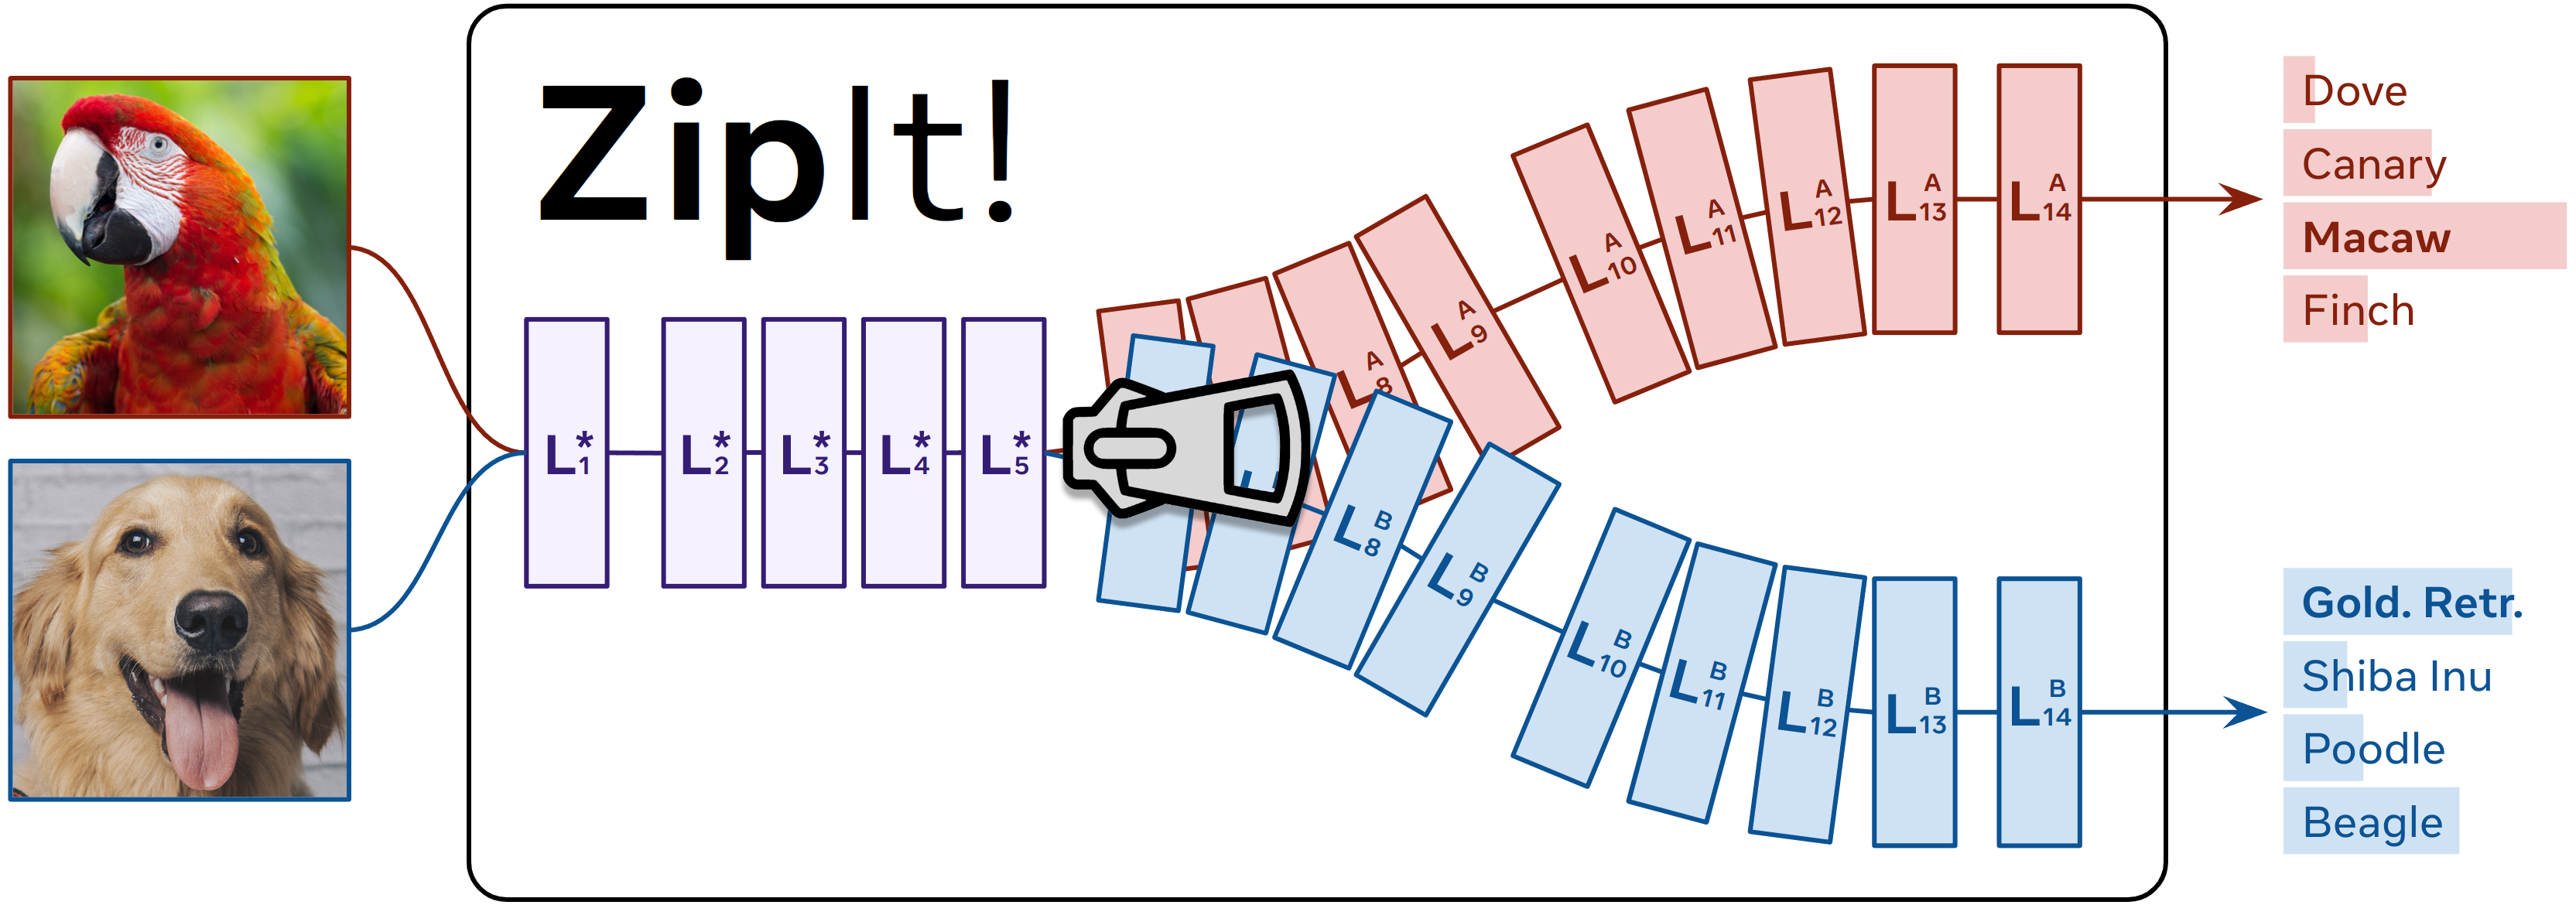
\includegraphics[width=\linewidth]{figures/imgs/concept.png}
%     \caption{{\bf \name{}} merges models trained on completely separate tasks \textit{without any additional training} by identifying their shared features.
%     Depending on the architecture and task, \name{} can nearly match their ensemble performance.
%     }
%     \label{fig:concept}
% }\end{minipage}
% \hspace{1em}
% \begin{minipage}{0.48\linewidth}{
%     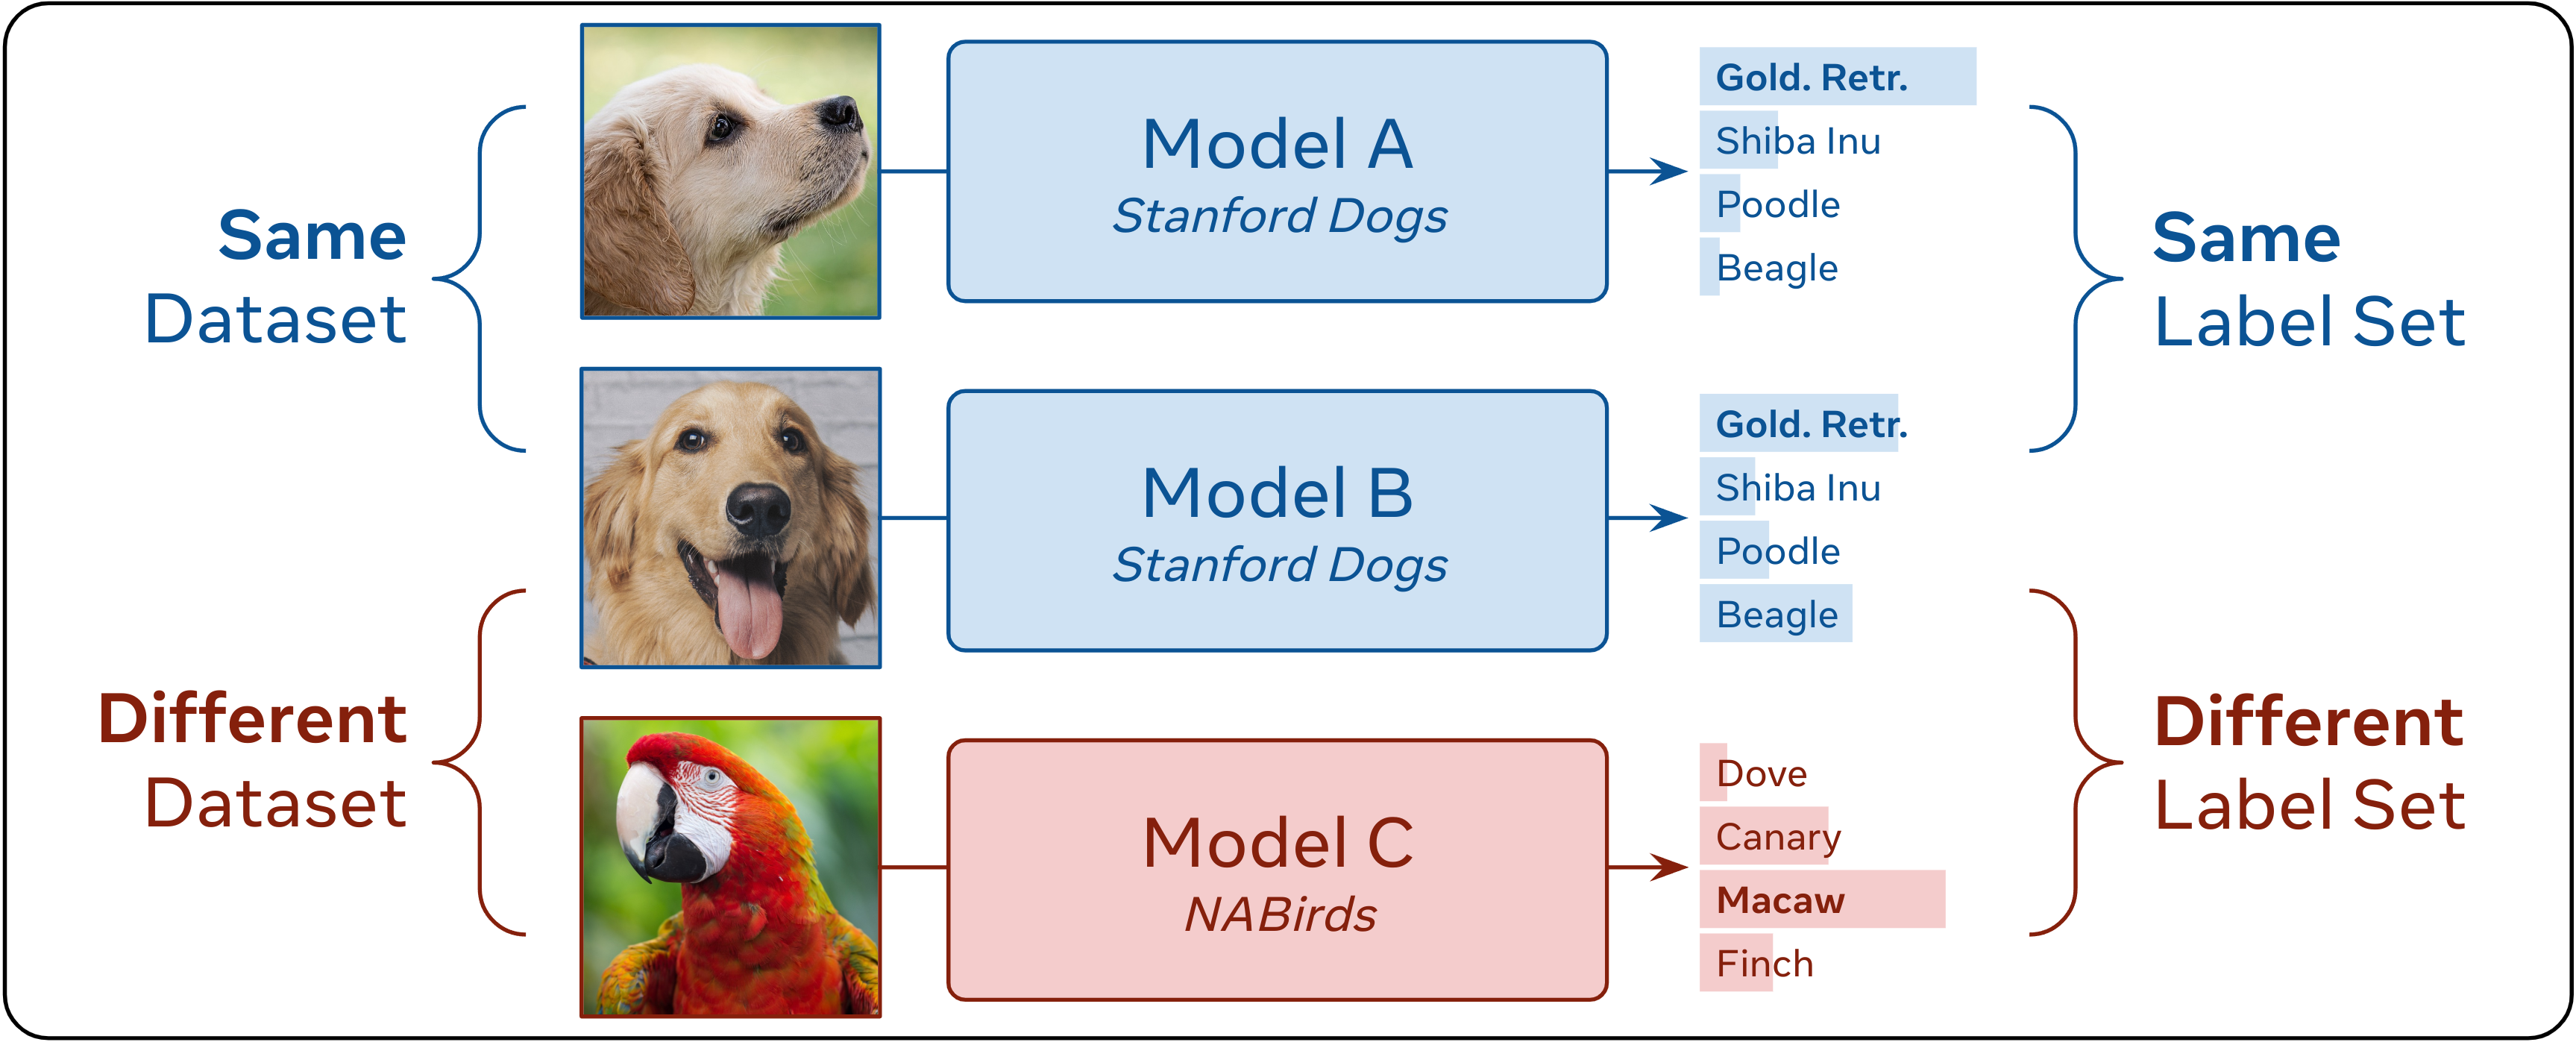
\includegraphics[width=\linewidth]{figures/imgs/vs_prior_work.png}
%     \caption{{\bf Our Setting.} Prior work \cite{wortsman2022model,ainsworth2022git,jordan2022repair}
%     focuses on merging models from the \modelb{\textbf{same} dataset} with the \modelb{\textbf{same} label sets}: e.g., merging two models both trained to classify dog breeds. In this work, we remove that restriction and ``zip'' models that can come from \modela{\textbf{different} datasets} and have \modela{\textbf{different} label sets}: e.g., merging a model that classifies dog breeds with one that classifies bird species.
%     }
%     \label{fig:capabilities}
%     % \includegraphics[width=\linewidth]{figures/imgs/random_r_experiment.png}
    
%     % \captionof{figure}{\textbf{Token Merging Schedule.} Our default constant merging schedule is close to optimal when compared to 15k randomly sampled merging schedules on an AugReg ViT-B/16. }
%     % \label{fig:r_ablation}
% }\end{minipage}
% \end{figure}




\begin{figure}[t]
\centering
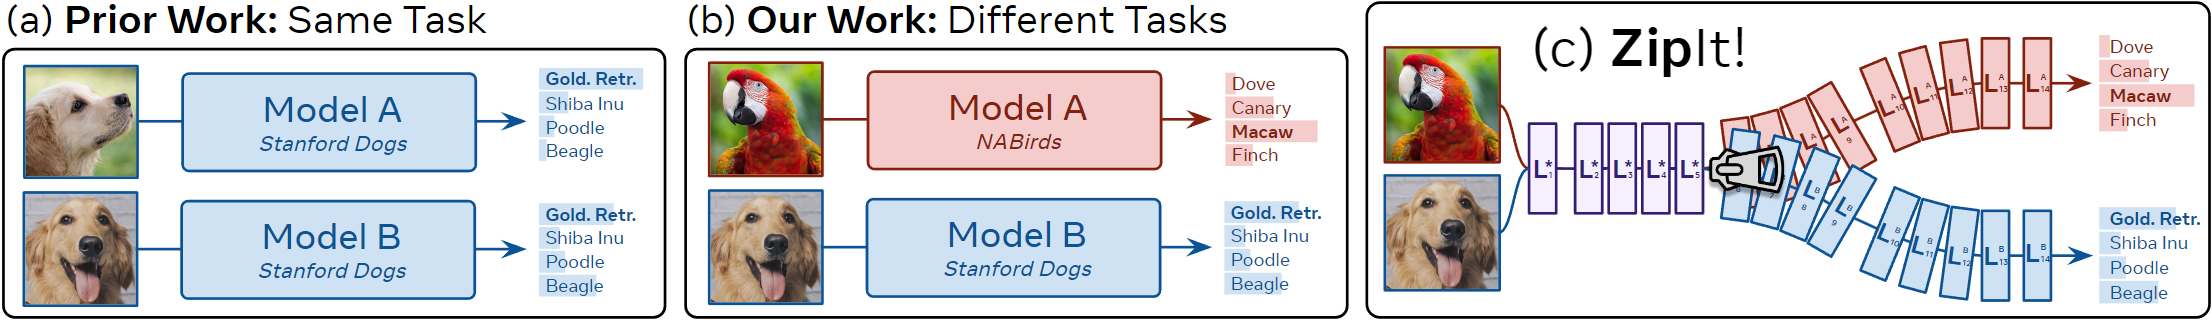
\includegraphics[width=\linewidth]{figures/imgs/concept_and_capabilities.png}
    \caption{
    {\bf Setting and \name{}} (a) Prior work merges differently initialized models from the \modelb{\textbf{same} dataset} with the \modelb{\textbf{same} label sets}: e.g., merging two models both trained to classify dog breeds. (b) Our setting expands this to merging models from \modela{\textbf{different} datasets} with \modela{\textbf{different} label sets}: e.g., merging a model that classifies dog breeds with one that classifies bird species. (c) {\bf \name{}}\ merges these models \textit{without retraining} by identifying shared features.
    }
    \label{fig:concept_and_capabilities}
\end{figure}




% However, while these deep models are extremely powerful, they suffer from a potentially debilitating issue: they can only perform the task they were trained on. If we want to expand an existing model's capabilities, we run into many potential issues. If we try training the model on an additional task, we face catastrophic forgetting \cite{kirkpatrick2017overcoming,li2017learning,de2021continual}. If we evaluate the same model on different data without adaptation, we often find it doesn't generalize to out of domain samples \cite{blanchard2011generalizing,muandet2013domain,wang2022generalizing}. We can try so called ``intervention'' strategies \cite{wang2022generalizing,de2021continual} to mitigate these effects, but these often require further training which can be expensive.
% 


% \begin{figure}[b]
% \centering

% \begin{minipage}{0.48\linewidth}{
%     % \centering
%     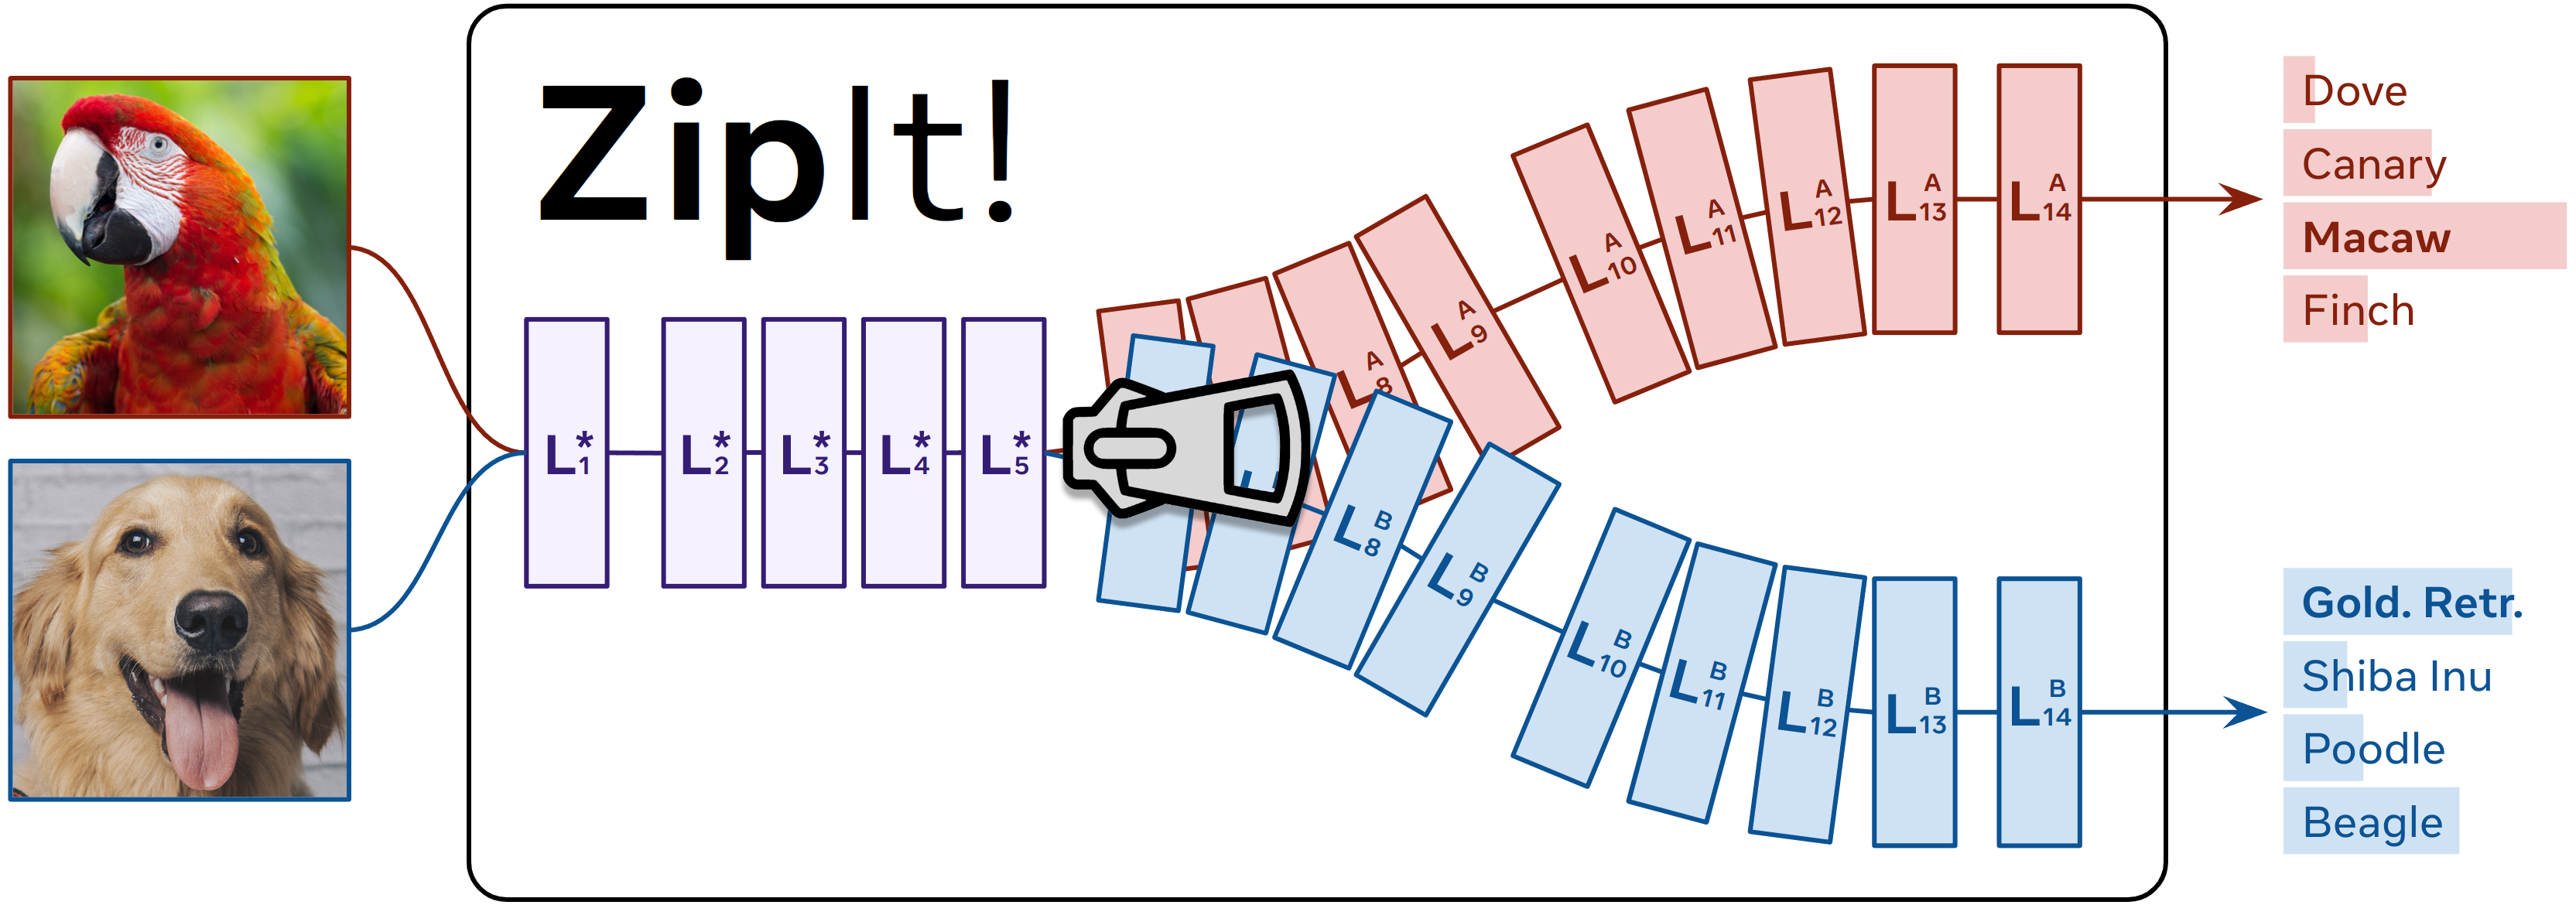
\includegraphics[width=\linewidth]{figures/imgs/concept.png}
%     \caption{{\bf \name{}} merges models trained on completely separate tasks \textit{without any additional training} by identifying their shared features.
%     Depending on the architecture and task, \name{} can nearly match their ensemble performance.
%     }
%     \label{fig:concept}
% }\end{minipage}
% \hspace{1em}
% \begin{minipage}{0.48\linewidth}{
%     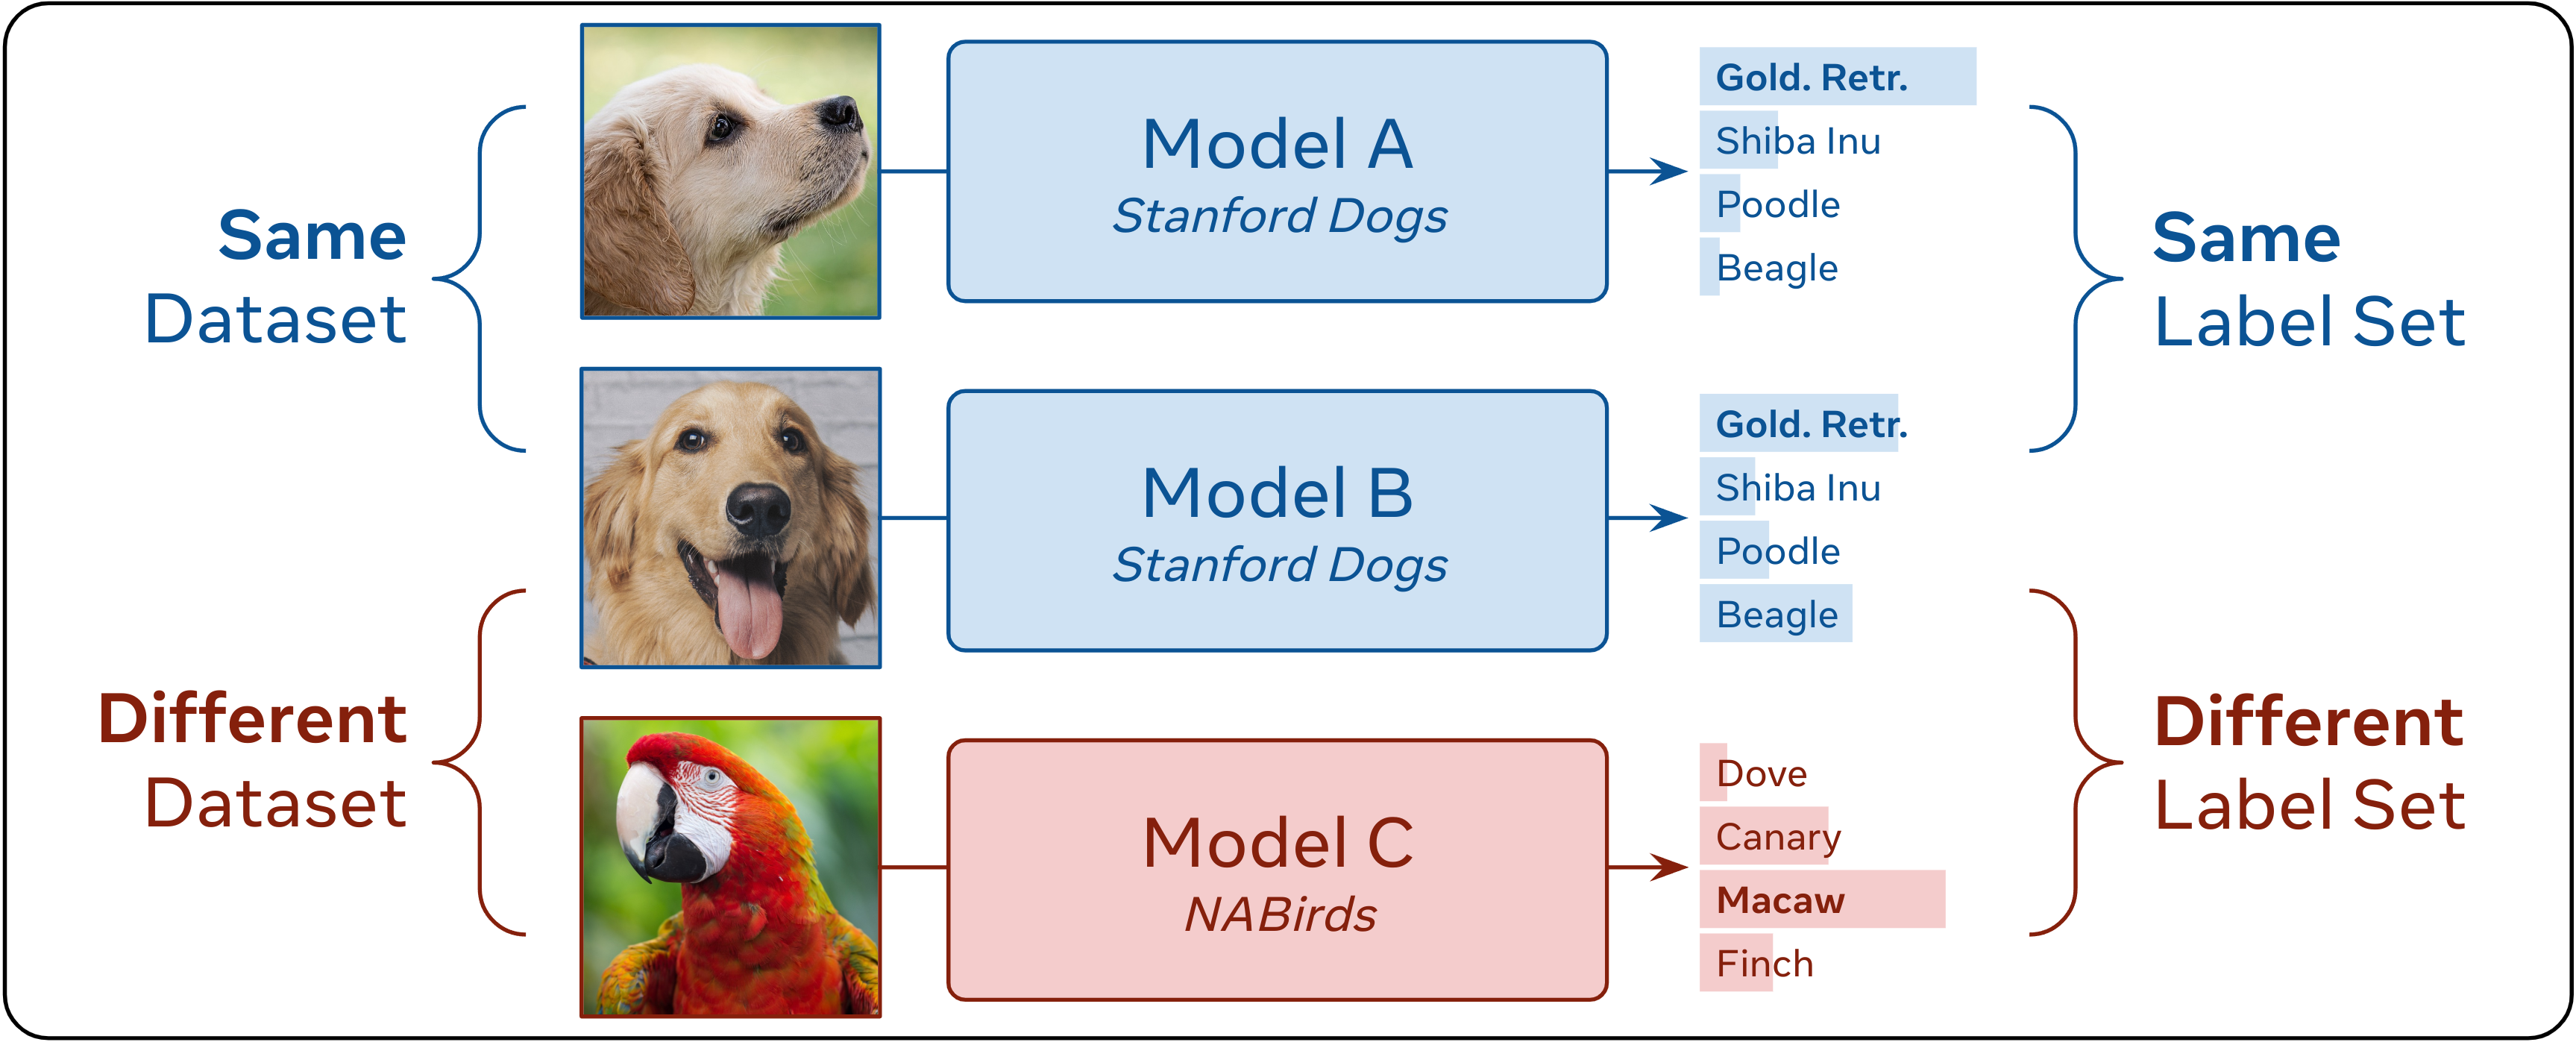
\includegraphics[width=\linewidth]{figures/imgs/vs_prior_work.png}
%     \caption{{\bf Our Setting.} Prior work \cite{wortsman2022model,ainsworth2022git,jordan2022repair}
%     focuses on merging models from the \modelb{\textbf{same} dataset} with the \modelb{\textbf{same} label sets}: e.g., merging two models both trained to classify dog breeds. In this work, we remove that restriction and ``zip'' models that can come from \modela{\textbf{different} datasets} and have \modela{\textbf{different} label sets}: e.g., merging a model that classifies dog breeds with one that classifies bird species.
%     }
%     \label{fig:capabilities}
%     % \includegraphics[width=\linewidth]{figures/imgs/random_r_experiment.png}
    
%     % \captionof{figure}{\textbf{Token Merging Schedule.} Our default constant merging schedule is close to optimal when compared to 15k randomly sampled merging schedules on an AugReg ViT-B/16. }
%     % \label{fig:r_ablation}
% }\end{minipage}
% \end{figure}




\begin{figure}[t]
\centering
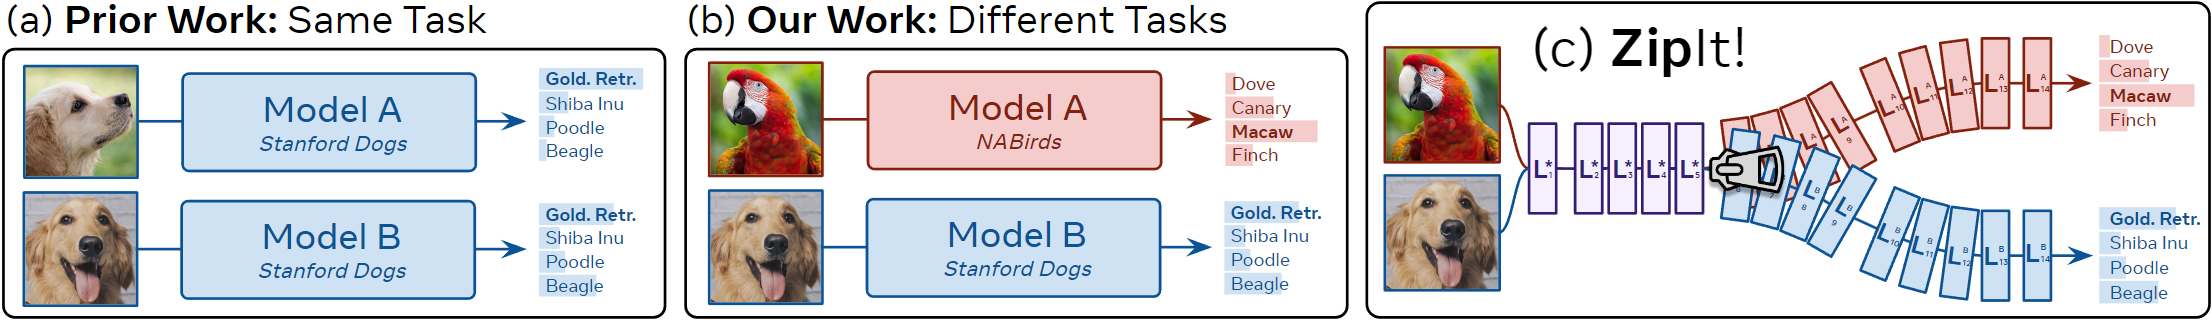
\includegraphics[width=\linewidth]{figures/imgs/concept_and_capabilities.png}
    \caption{
    {\bf Setting and \name{}} (a) Prior work merges differently initialized models from the \modelb{\textbf{same} dataset} with the \modelb{\textbf{same} label sets}: e.g., merging two models both trained to classify dog breeds. (b) Our setting expands this to merging models from \modela{\textbf{different} datasets} with \modela{\textbf{different} label sets}: e.g., merging a model that classifies dog breeds with one that classifies bird species. (c) {\bf \name{}}\ merges these models \textit{without retraining} by identifying shared features.
    }
    \label{fig:concept_and_capabilities}
\end{figure}


% There are
% %,  of course, 
% a plethora of existing, carefully tuned models out there for many tasks. But despite these models often sharing the same core architectural backbone (e.g., ResNet-50~\cite{he2015deep}), no method yet exists that can easily combine models trained on disjoint tasks. We're either stuck ensembling them, which requires evaluating each model individually, or jointly training a new model through distillation~\cite{li2020knowledge}. Both can be prohibitively expensive with the modern trend of ever increasing architecture and dataset scales \cite{dosovitskiy2020image,zhai2022scaling,dehghani2023scalingvit22b}.
% Instead, it would be nice if we could simply ``zip'' these models together so that any redundant features between them only need to be computed once, \textit{without} any additional training.

% Recently, the idea of combining multiple models into one has started to gain traction in the vision community. 
Combining multiple models into one has recently started to gain traction in the vision community.
Model Soups \cite{wortsman2022model} can add multiple models finetuned from the same pretrained initialization to improve accuracy and robustness. Git Re-Basin \cite{ainsworth2022git} generalizes further to models trained on the same data but with different initializations, though with a significant accuracy drop. REPAIR \cite{jordan2022repair} improves on Git Re-Basin by adding new parameters and adjusting model batch norms where applicable.
However, all of these methods only combine models trained on the same task.
In this paper, we take this line of work to a logical extreme: merging differently initialized models trained on \textit{completely separate} tasks (see Fig.~\ref{fig:concept_and_capabilities}\hyperref[fig:concept_and_capabilities]{ab}).
% While 
We show
that this is an incredibly difficult problem for prior work 
% we 
and
employ two simple strategies to make it feasible.

First, we note that prior work focuses on \textit{permuting} one model to the other when merging them. This creates a 1-1 mapping between the two models, inherently assuming that most features \textit{across} them are correlated. Since this isn't necessarily the case for models trained on different tasks, we cannot rely on permutation alone. 
Instead, we generalize model merging to support ``zipping'' any combination of correlated features \textit{within} and \textit{across} each model.
% Instead, we exploit redundancy \textit{within} each model as well. 
% To do this, we generalize model merging to support ``zipping'' any combination of features \textit{within} and \textit{across} each model.
We find that on some tasks, this alone improves accuracy \textbf{by up to 20\%} vs. 
permutation-based approaches.
% Git Re-basin \cite{ainsworth2022git} applied in this setting and an even stronger permutation baseline that we implement.
Moreover, we prove that merging within models can yield a better result in the theoretical setting of \citet{entezari2021role}.

Second, existing methods merge \textit{the entire network}. While this might work for extremely similar models trained in the same setting, the features of models trained on disjoint tasks become less correlated over the course of the network \cite{kornblith2019similarity}. To solve this, we introduce \textit{partial zipping}, where we only ``zip'' up to a specified layer. Afterward, we feed the merged model's outputs to the remaining unmerged layers of the original networks, creating a multi-head model. Depending on task difficulty, this can improve accuracy \textbf{by over 15\%} while still keeping most layers merged.


Incorporating both of these strategies, we introduce \name{}\ (Fig.~\ref{fig:concept_and_capabilities}\hyperref[fig:concept_and_capabilities]{c}), a general method for ``zipping'' any number of models trained on different tasks into a single multitask model \textit{without retraining}.
By deriving a general graph-based algorithm for merging and unmerging (Sec.~\ref{sec:approach}), we can zip models of the same architecture together, 
merge features \textit{within} each model,
and partially zip them to create a multi-task model.
We validate our approach by merging models trained on entirely disjoint sets of CIFAR \cite{krizhevsky2009cifar} and ImageNet \cite{deng2009imagenet} categories, as well as merging several models trained on completely independent datasets into one, significantly outperforming prior work (Sec.~\ref{sec:results}). 
Finally, we ablate and analyze our method's capabilities on these scenarios (Sec.~\ref{sec:ablations}).

\section{Related Work} \label{sec:related_work}
Model merging combines the weights of two or more models into a one. Our work differs from prior work in that we adapt mode connectivity techniques to target models trained on disjoint tasks (Fig.~\ref{fig:concept_and_capabilities}).
 

\paragraph{Merging Finetuned Models.}
If two models are finetuned from the same pretrained checkpoint, they often lie in the same error basin \cite{neyshabur2020being}. 
Several works~\cite{huang2017snapshot,izmailov2018averaging,von2020neural,wortsman2022robust,ilharco2022patching,donyehiya2023cold} have exploited this property to average together the weights of a model at different stages of training. 
\citet{tarvainen2017mean,cai2021exponential,grill2020bootstrap,caron2021emerging,baevski2022data2vec} use an ``exponential moving average'' of training checkpoints as a teacher for self-supervised learning.
Other works merge models initialized from the same pretrained base, but that were finetuned independently, either by simply averaging their weights \cite{mcmahan2017communication,wortsman2022model,choshen2022fusing,rame2022recycling}, permuting one model to the other \cite{ashmore2015method,yurochkin2019bayesian,wang2020federated}, combining meaningful weight regions \cite{ilharco2022editing, gueta2023knowledge,yadav2023resolving,sung2023empirical}, or maximizing an objective \cite{matena2021merging}. Our setting differs, as we do not assume the same initialization.

\vspace{-0.2em}
\paragraph{Merging Differently Initialized Models.}
Merging models with different initializations is a much more challenging problem. 
Works in this space often rely on \textit{mode connectivity} \cite{freeman2016topology,garipov2018loss,draxler2018essentially,frankle2020linear}, attempting to interpolate between models along a low loss path (e.g., \citet{tatro2020optimizing,singh2020model,liu2022deep}).
Most recent work follow the intuition, later formalized by \citet{entezari2021role}, that models permuted to the same loss basin can be merged by averaging their weights. Most notably, Git Re-Basin \cite{ainsworth2022git} permutes models
% locally, primarily
by comparing the similarity between their weights. REPAIR \cite{jordan2022repair} improves the accuracy of Git Re-Basin by instead computing the correlation between their intermediate layer feature activations, and adding several batch norms to the network. \citet{pena2022re} find permutations using global rather than local optimization, though they don't support skip connections.
% Interestingly, an alternative method using the Hessian of the forward features \cite{he2018multi} exists, which outperforms other permutation-based approaches (\citet{entezari2021role} Appendix B). However, the most recent work  in this area \cite{ainsworth2022git,jordan2022repair} do not use this technique, so we operate in the (more limited) correlation-based domain of \citet{jordan2022repair}.
% \citet{he2018multi} uses the Hessian of the forward features to merge models of different tasks but with intermediate finetuning.\footnote{Note: \citet{he2018multi} claim to include experiments without retraining, but according to their code they perform sequential iterations of merging and finetuning for each merged layer. Their ``without retraining'' experiments mean the \textit{most recent} merged layer isn't finetuned, but the rest are.}
Some of these works (e.g., \citet{singh2020model,ainsworth2022git}) evaluate on on a setting where each model sees varying numbers of instances per class. And \citet{pena2022re} evaluates on a continual learning setting with disjoint categories, but their method requires training optimization.
Similarly, \citet{he2018multi} merges models of different tasks, but requires jointly finetuning after each layer merge.
As far as we are aware, we present the first \textit{general method} to successfully merge models trained on disjoint tasks \textit{without additional training}.

% Nevertheless, all prior work only consider merging \textit{across} models. Instead, we merge both \textit{within} and \textit{across} models \textit{without retraining}.
 
 % Unlike prior work, however, we present a \textit{general method} to merge both \textit{within} and \textit{across} multiple models trained on disjoint tasks \textit{without retraining}.
 
 % Our focus in this work is to present a \textit{general method} of merging models trained on disjoint tasks \textit{without retraining} by allowing features to be merged \textit{within} models.
 % To our knowledge, we are the first to present a \textit{general method} to successfully merge models trained on disjoint tasks \textit{without training} by allowing features to be merged \textit{within} models.

% Some of these works (e.g., \citet{singh2020model,ainsworth2022git,liu2022deep}) evaluate on on a setting where each model sees varying numbers of instances per class. And \citet{pena2022re} evaluates on a continual learning setting where models are given disjoint categories, but their method requires training optimization and does not support skip connections.

% Finally, an alternative method using the Hessian of the features \cite{he2018multi} exists, which outperforms correlation-based approaches (\citet{}

% \textcolor{red}{Finally, \citet{he2018multi}.} s
% As far as we are aware, we present the first \textit{general method} to successfully merge models trained on disjoint tasks \textit{without retraining}.


% \paragraph{new draft of related works work in progress by Jakob}
% Models of increasing size are being trained as pre-trained checkpoints for downstream tasks (citation). Model soups (citation) took many fine-tuned models from the same pre-trained checkpoint and linearly averaged them to achieve better performance on the fine-tuning task. Other works have recombined and again fine-tuned to improve accuracy and robustness (citation to Model Ratatouille, ColD fusion?, Fusing Finetuned models for better pretraining?, knowledge is a region in weight space for FT models [TODO: check notes for if these are the right to cite]). Along the lines of experimenting with fine-tuned models from the same pre-trained checkpoint, prior works experiment with the addition of different weight vectors to represent performance different tasks (editing Models with task arithmetic, resolving interference when merging models? [TODO: check citation]).

% A very relevant work "Multi-Task Zipping via Layer-wise Neuron Sharing" (citation) seeks to merge models' weights depending on which neurons in the models represent shared information. This work differs in that they increase the model's footprint, and don't allow for intra model merging. (These are not really limitations, as they increase the accuracy substantially for this prior work, Need to discuss in person about this work for how to best address it in the paper.)

% Mechanistic Mode Connectivity should be looked at more closely. Didn't have time.

% Patching open vocab didn't look at no time.




% %%%%%%%%%%% Prior version 9/23/2023

% \section{Related Work} \label{sec:related_work}
% Model merging combines the weights of two or more models into a single set of weights.
% % in a useful way. 
% Our work differs from prior work by explicitly targeting models that have been trained on disjoint tasks (Fig.~\ref{fig:concept_and_capabilities}).
% % In this work, we explicitly target models that have been trained on disjoint tasks (Fig.~\ref{fig:concept_and_capabilities}), which differs from prior work.

% \paragraph{Merging Finetuned Models.}
% If two models are finetuned from the same pretrained checkpoint, they often lie in the same error basin \cite{neyshabur2020being}. 
% Several works~\cite{huang2017snapshot,izmailov2018averaging,von2020neural,wortsman2022robust} have exploited this property to average together the weights of a model while training. 
% \cite{tarvainen2017mean,cai2021exponential,grill2020bootstrap,caron2021emerging,baevski2022data2vec} use an ``exponential moving average'' of training checkpoints as a teacher for self-supervised learning.
% Other works merge models initialized from the same pretrained base, but that were fine-tuned independently, either by simply averaging their weights \cite{mcmahan2017communication,wortsman2022model}, permuting one model to the other \cite{ashmore2015method,yurochkin2019bayesian,wang2020federated}, or maximizing some objective \cite{matena2021merging}. Our setting differs, as we do not assume the same initialization.

% \vspace{-0.2em}
% \paragraph{Merging Differently Initialized Models.}
% Merging models with different initializations is a much more challenging problem. 
% Works in this space often rely on \textit{\textcolor{red}{linear} mode connectivity} \cite{freeman2016topology,garipov2018loss,draxler2018essentially,frankle2020linear}, attempting to interpolate between models along a low loss path (e.g., \citet{tatro2020optimizing,singh2020model,liu2022deep}). The most popular approach follows
% the intuition, later formalized by \citet{entezari2021role}, that models permuted to the same loss basin can be merged by averaging their wights. Most notably, Git Re-Basin \cite{ainsworth2022git} permutes models
% % locally, primarily
% by comparing the similarity between their weights. REPAIR \cite{jordan2022repair} improves the accuracy of Git Re-Basin by instead computing the similarity between their intermediate layer feature activations, and adding several batch norms to the network. \cite{pena2022re} finds permutations using global rather than local optimization, though the method doesn't generalize well to modern architectures. Some of these works (e.g., \citet{singh2020model,ainsworth2022git,liu2022deep}) evaluate on on a setting where each model sees varying numbers of instances per class. And one concurrent work \cite{pena2022re} evaluates on a continual learning setting where models are given disjoint categories, but their method requires optimization and does not support skip connections. As far as we are aware, we present the first \textit{general method} to successfully merge models trained on disjoint tasks \textit{without retraining}.

% Our goal is to merge any models of the same architecture together \textit{without additional training}. Unlike prior work \cite{wortsman2022model,ainsworth2022git,jordan2022repair}, we specifically target the extremely difficult setting of models that have different initializations and are trained on completely different tasks. In this section, we will motivate the need for a new approach by showing how prior work fails on this challenging setting.

% \paragraph{What constitutes a task?}
% The term ``task'' is often overloaded in machine learning. The broader vision community treats ``tasks'' as different problem statements (e.g., detection vs. segmentation \cite{lin2014coco}), while subfields like continual learning \cite{de2021continual} define ``tasks'' as disjoint category splits of the same data. While we would ideally support any definition, we specifically focus on classification in this work. We define tasks as either disjoint category splits of the same data or as classification on different datasets entirely.

% \subsection{Background}
% Consider a model $\mathcal{L}$ as a collection of layers $L_i \in \mathcal{L}$, each of which may have some parameters (e.g., $W_i, b_i$ for a linear layer). 
% If \modela{$\mathcal{L}^A$} and \modelb{$\mathcal{L}^B$} are finetuned from the same checkpoint, several works (e.g., \cite{huang2017snapshot,izmailov2018averaging,wortsman2022model}) have found that merging them is as easy as averaging their weights. For instance, if $L_i$ is a linear layer, the new weight matrix \modelc{$W_i^*$} is simply
% \begin{equation} \label{eq:wavg}
%     % \modelc{W_i^*} = \modela{\frac{1}{2} W_i^A} + \modelb{\frac{1}{2} W_i^B}
%     \modelc{W_i^*} = \gamma\modela{W_i^A} + (1-\gamma)\modelb{W_i^B}
% \end{equation}
% \textcolor{blue}{where $\gamma\in[0,1]$ and is usually set to $\frac{1}{2}$.} 
% However, if \modela{$\mathcal{L}^A$} and \modelc{$\mathcal{L}^B$} were not finetuned from the same checkpoint, Eq.~\ref{eq:wavg} typically results in random accuracy
% To fix this, a line of work (most recently \cite{ainsworth2022git,jordan2022repair}) has found that if you first permute the feature space of one model to align with the feature space of the other model before averaging them together, you can recover much of the lost accuracy. More concretely, let \modelb{$P_i$} be a permutation matrix that permutes the output of layer \modelb{$L_i^B$} to the space of \modela{$L_i^A$}. Then for each layer, works such as Git Re-Basin \cite{ainsworth2022git} apply
% \begin{equation} \label{eq:rebasin}
%     % \modelc{W_i^*} = \modela{\frac{1}{2} W_i^A} + \modelb{\frac{1}{2} P_i W_i^B P_{i-1}^T}
%     \modelc{W_i^*} = \gamma\modela{W_i^A} + (1-\gamma)\modelb{ P_i W_i^B P_{i-1}^T}
% \end{equation}
% Note that here we permute the output space of \modelb{$W_i^B$}, but we also need to permute its input space to undo the permutation from the previous layer (hence the use of \modelb{$P_{i-1}^T$}).

% 
% \begin{wrapfigure}{r}{0.48\textwidth}
%   \vspace{-20pt}
%   \centering
%   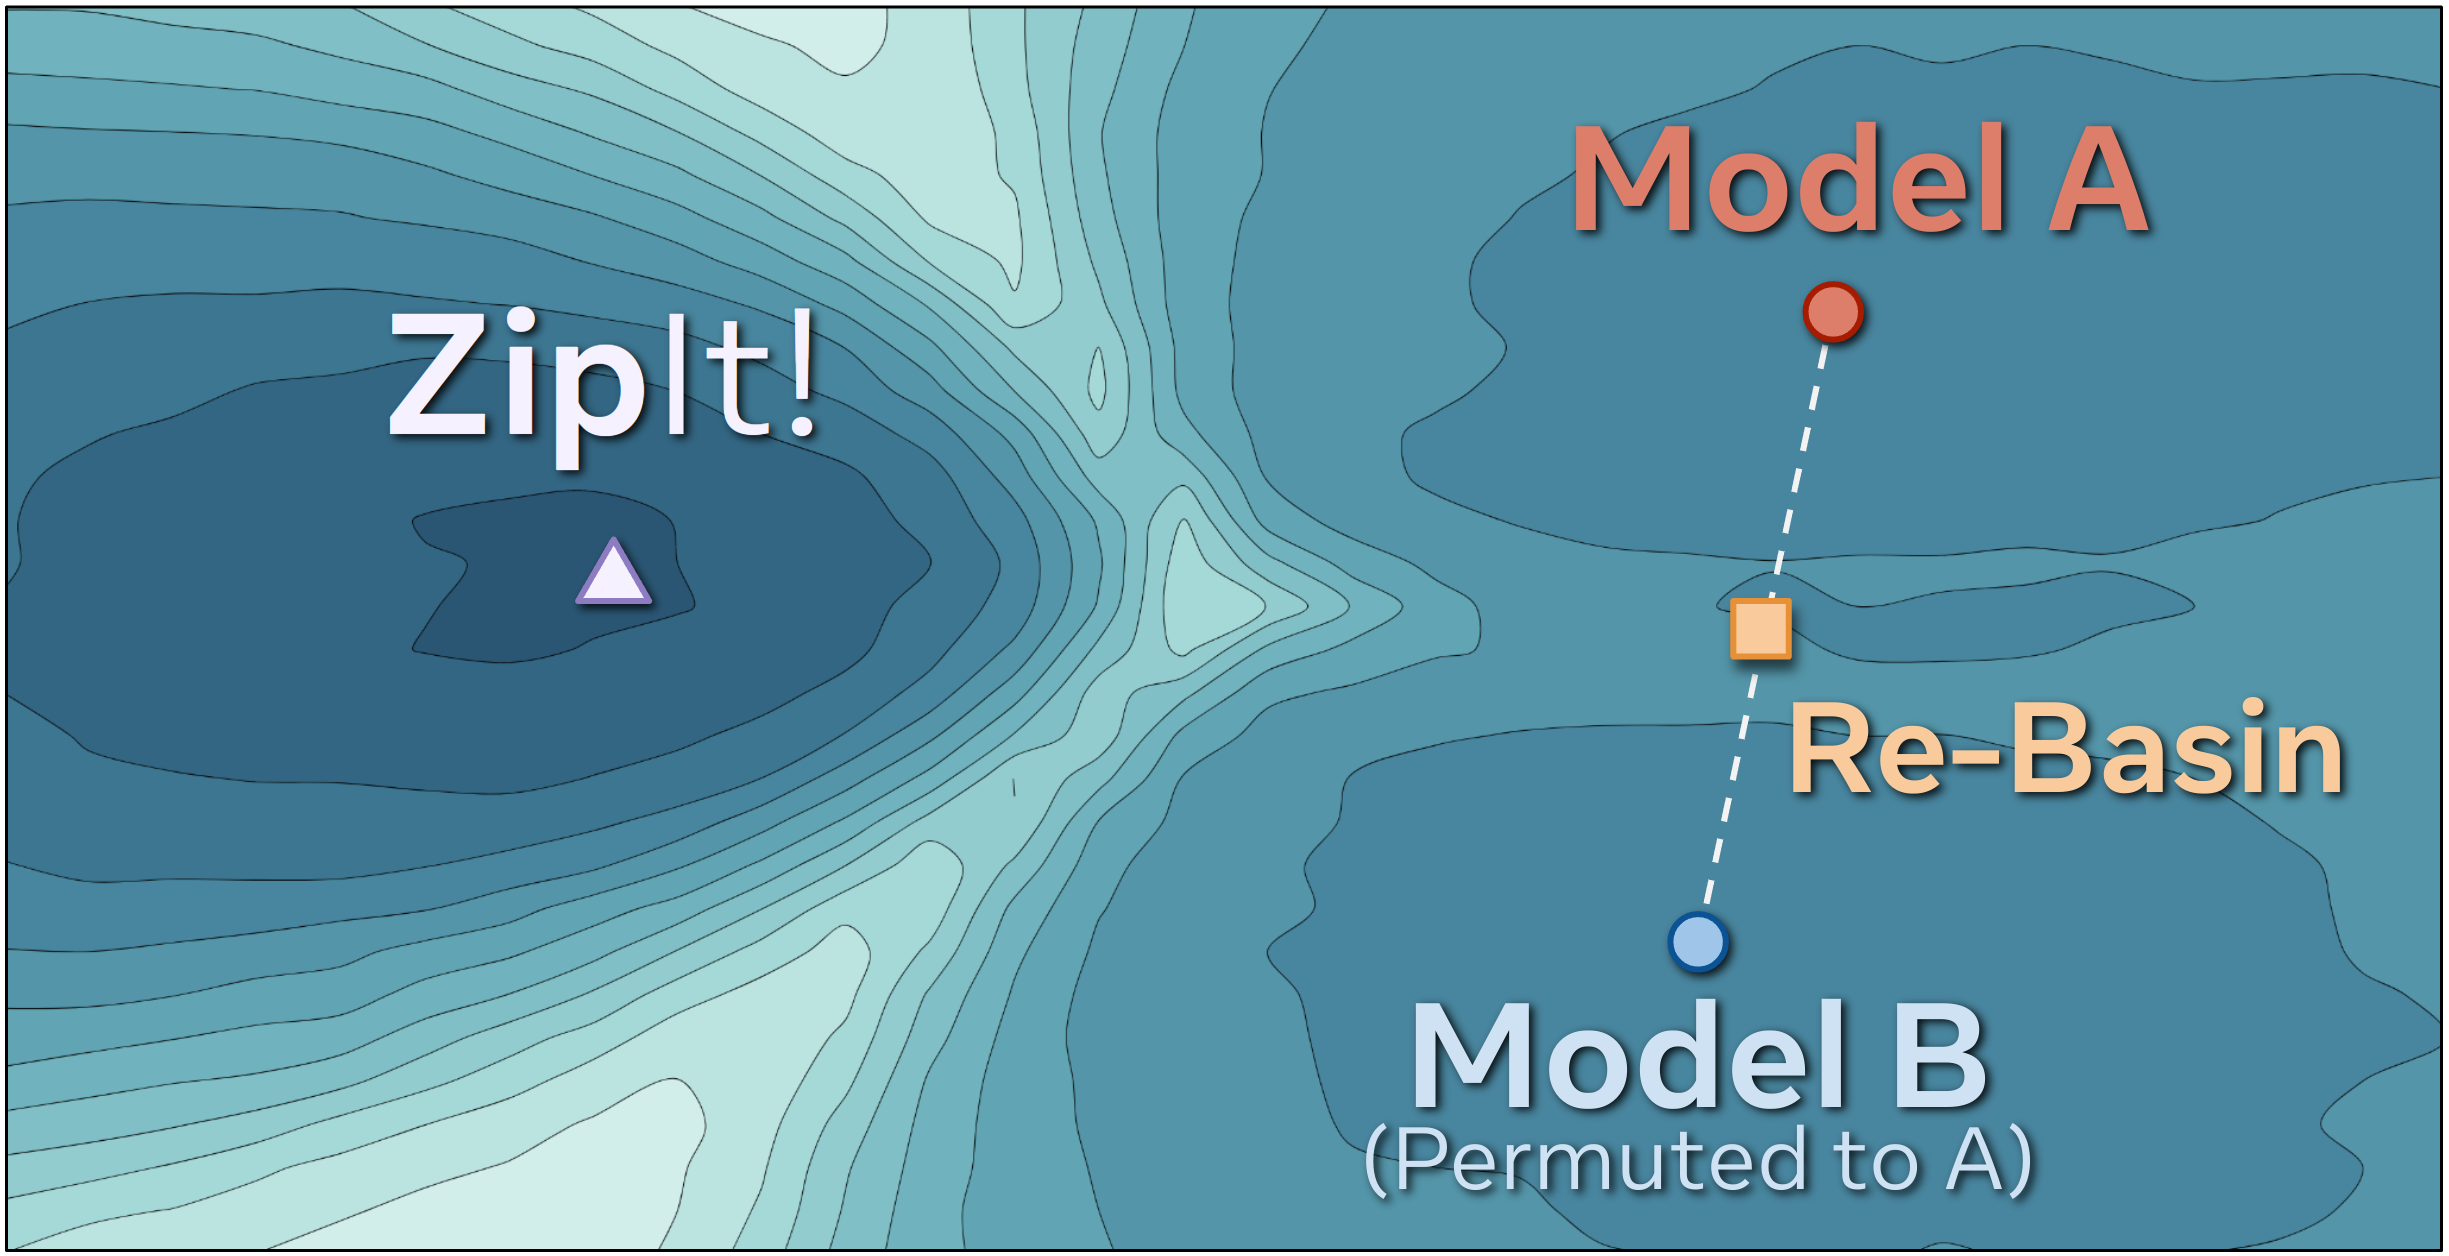
\includegraphics[width=\linewidth]{figures/imgs/loss_basin.png}
%   \newline
%   \caption{{\bf Prior Work Fails} on merging models trained on \textit{different} tasks. Git Re-Basin \cite{ainsworth2022git} assumes the two models lie in the same loss basin \textit{modulo permutation} and interpolates between them. However, that is not sufficient when the models are trained on \textit{different} tasks, here shown for disjoint class sets of CIFAR-100. While \modela{A} and the permuted \modelb{B} lie in similar basins, Git Re-Basin's interpolation performs \textit{worse} than the originals. In contrast, our method \name\ merges them into an even better model in a completely different loss basin.}
%   \label{fig:loss_basin}
%   \vspace{-50pt}
% \end{wrapfigure}



\begin{figure}
  \centering
  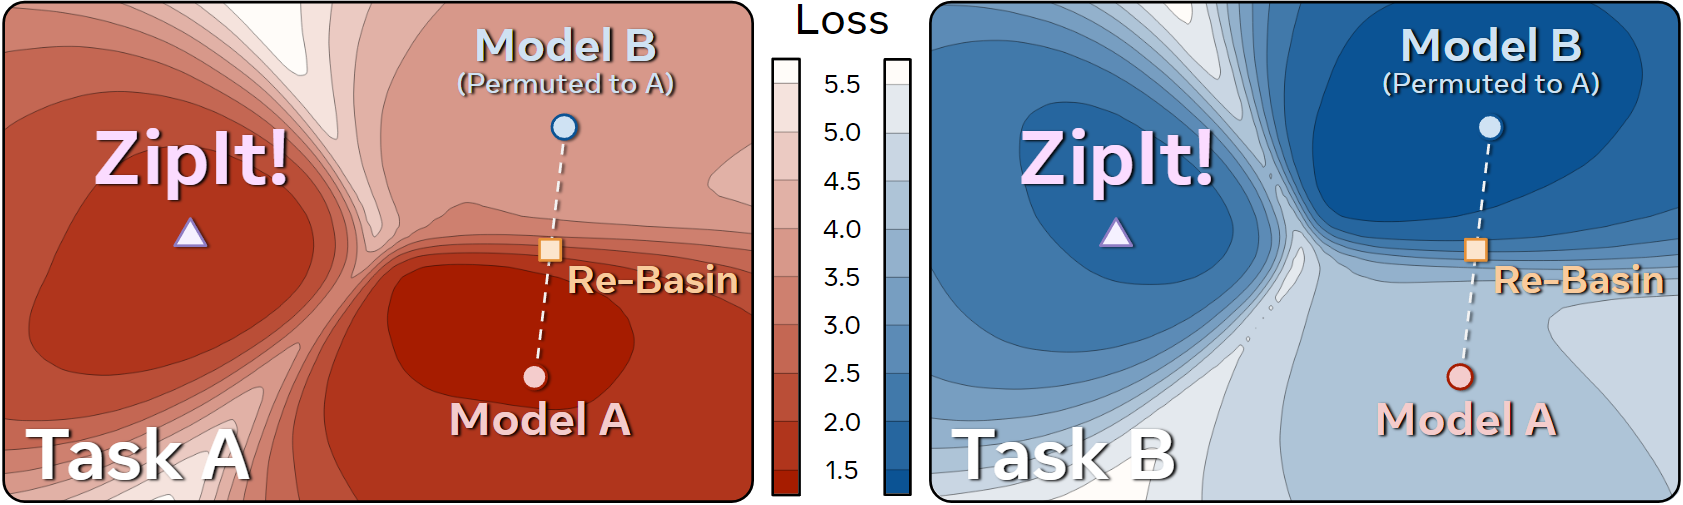
\includegraphics[width=\linewidth]{figures/imgs/loss_landscapes.png}
  % \newline
  % \vspace{-0.5em}
  \caption{{\bf Task Loss Landscapes} for models in Tab.~\ref{tab:cifar50+50}. % Prior work fails on merging models trained on different tasks: 
  \modela{Model A} and \modelb{Model B} lie in low loss basins for their own tasks, but \textit{not for the other task}.
  % While \modelb{Model B} lies in a low loss basin for \modelb{Task B}, it doesn't for \modela{Task A}, even after permuting it to \modela{Model A}.
  % because permuted models for \modela{Task A} likely \textit{do not} lie in a low loss basin for \modelb{Task B}.
  Thus, any interpolation between \modela{Model A} and a permuted \modelb{Model B} (e.g., Git Re-basin) lies outside the minima \textit{for both tasks} and thus performs poorly. In contrast, \name{}\ improves the merge by finding a model that lies in a low loss basin for both.
  % by finding a loss basin common to both tasks.
  % Git Re-Basin~\citet{ainsworth2022git} assumes the two models likely lie in the same loss basin \textit{modulo permutation} and interpolates between them. However, this is substantially less likely when the models are trained on \textit{different} tasks, here shown for disjoint class sets of CIFAR-100. While \modela{A} and \modelb{B} lie in basins on their respective tasks, these \textit{are not} shared across tasks. Thus, Git Re-Basin's interpolation performs \textit{worse} than the original's. In contrast, our method \name{}\ significantly improves the merge by finding a basin common to both tasks. 
  }
  \label{fig:loss_basin}
\end{figure}
% \paragraph{Problems with Permutation.}
% While Eq.~\ref{eq:rebasin} works decently well for models trained on the same task, its underlying assumptions break down when the models are trained on \textit{different} tasks. The idea of permutation-based model merging (e.g. Git Re-Basin \cite{ainsworth2022git}) stems from mode connectivity \cite{entezari2021role}, where it has been conjectured that models with different initializations trained on the same data lie in the same \textit{loss basin} (i.e., region of low loss or high accuracy) modulo permutation (as most neural networks can be permuted internally without affecting their outputs). As we show in Fig.~\ref{fig:loss_basin}, this does not hold in our setting where the two models are trained on different tasks. In this case, \modelb{Model B}'s optimal permutation lies in a \textit{similar} yet distinct basin to \modela{Model A}. Because the two models are actually in \textit{different basins}, the interpolated result actually has a \textit{lower} accuracy than either of the two original models. This motivates us to explore alternative methods for merging.

\section{Background and Motivation} \label{sec:motivation}

%%%%%%%%%%%%%%%%%%%%%%%%%%%%%%%%%%% NEW EDITS %%%%%%%%%%%%%%%%%%%%%%%%%%%%%%%%%%%
% The idea of 
Model merging stems from mode connectivity \cite{garipov2018loss}, where it is conjectured that models trained with SGD on the same dataset lying in the same \textit{loss basin} (i.e., region or \textit{mode} of low loss) can be combined into a single model that's just as performant as the original models. If these models can be combined well by linearly interpolating their weights, they are said to be \textit{linearly mode connected} (LMC) \cite{garipov2018loss,entezari2021role}. Our work is similar to finding LMC, but across \textit{different datasets with disjoint label sets} (i.e., separate tasks as in \citet{de2021continual}).

Consider a model $\mathcal{L}$ as a collection of layers $L_i \in \mathcal{L}$, each of which may have some parameters (e.g., $W_i, b_i$ for a linear layer). 
If \modela{$\mathcal{L}^A$} and \modelb{$\mathcal{L}^B$} are finetuned from the same checkpoint, several works (e.g., \citet{izmailov2018averaging,wortsman2022model}) find merging them is as easy as linearly interpolating their weights (i.e., they are LMC). E.g., if $L_i$ is a linear layer, the new weight matrix \modelc{$W_i^*$} is simply
\begin{equation} \label{eq:wavg}
    \modelc{W_i^*} = \gamma\modela{W_i^A} + (1-\gamma)\modelb{W_i^B}
\end{equation}
with an interpolation constant $\gamma\in[0,1]$, usually set to $\sfrac{1}{2}$. However, if \modela{$\mathcal{L}^A$} and \modelc{$\mathcal{L}^B$} were not finetuned from the same checkpoint, they often do not lie in the same mode \cite{entezari2021role, ainsworth2022git} and cannot be interpolated. Indeed, Eq.~\ref{eq:wavg} typically results in random accuracy. 

To fix this, \citet{entezari2021role} conjecture that \textit{large enough} models are likely LMC modulo permutation. This is because (1) many neural networks can be permuted internally without affecting their outputs and (2) permutation can move two models into the same basin, allowing much of the lost accuracy to be recovered.
% This is because permutations can move two models into the same basin without affecting their outputs, allowing much of the lost accuracy to be recovered.
More concretely, let \modelb{$P_i$} be a permutation matrix that permutes outputs of layer \modelb{$L_i^B$} to the space of \modela{$L_i^A$}. Then for each layer, permutation works 
% such as Git Re-Basin \cite{ainsworth2022git} 
apply
\begin{equation} \label{eq:rebasin}
    % \modelc{W_i^*} = \modela{\frac{1}{2} W_i^A} + \modelb{\frac{1}{2} P_i W_i^B P_{i-1}^T}
    \modelc{W_i^*} = \gamma\modela{W_i^A} + (1-\gamma)\modelb{ P_i W_i^B P_{i-1}^T}
\end{equation}
Note that here we permute the output space of \modelb{$W_i^B$}, but we also need to permute its input space to undo the permutation from the previous layer (hence the use of \modelb{$P_{i-1}^T$}).


% \begin{wrapfigure}{r}{0.48\textwidth}
%   \vspace{-20pt}
%   \centering
%   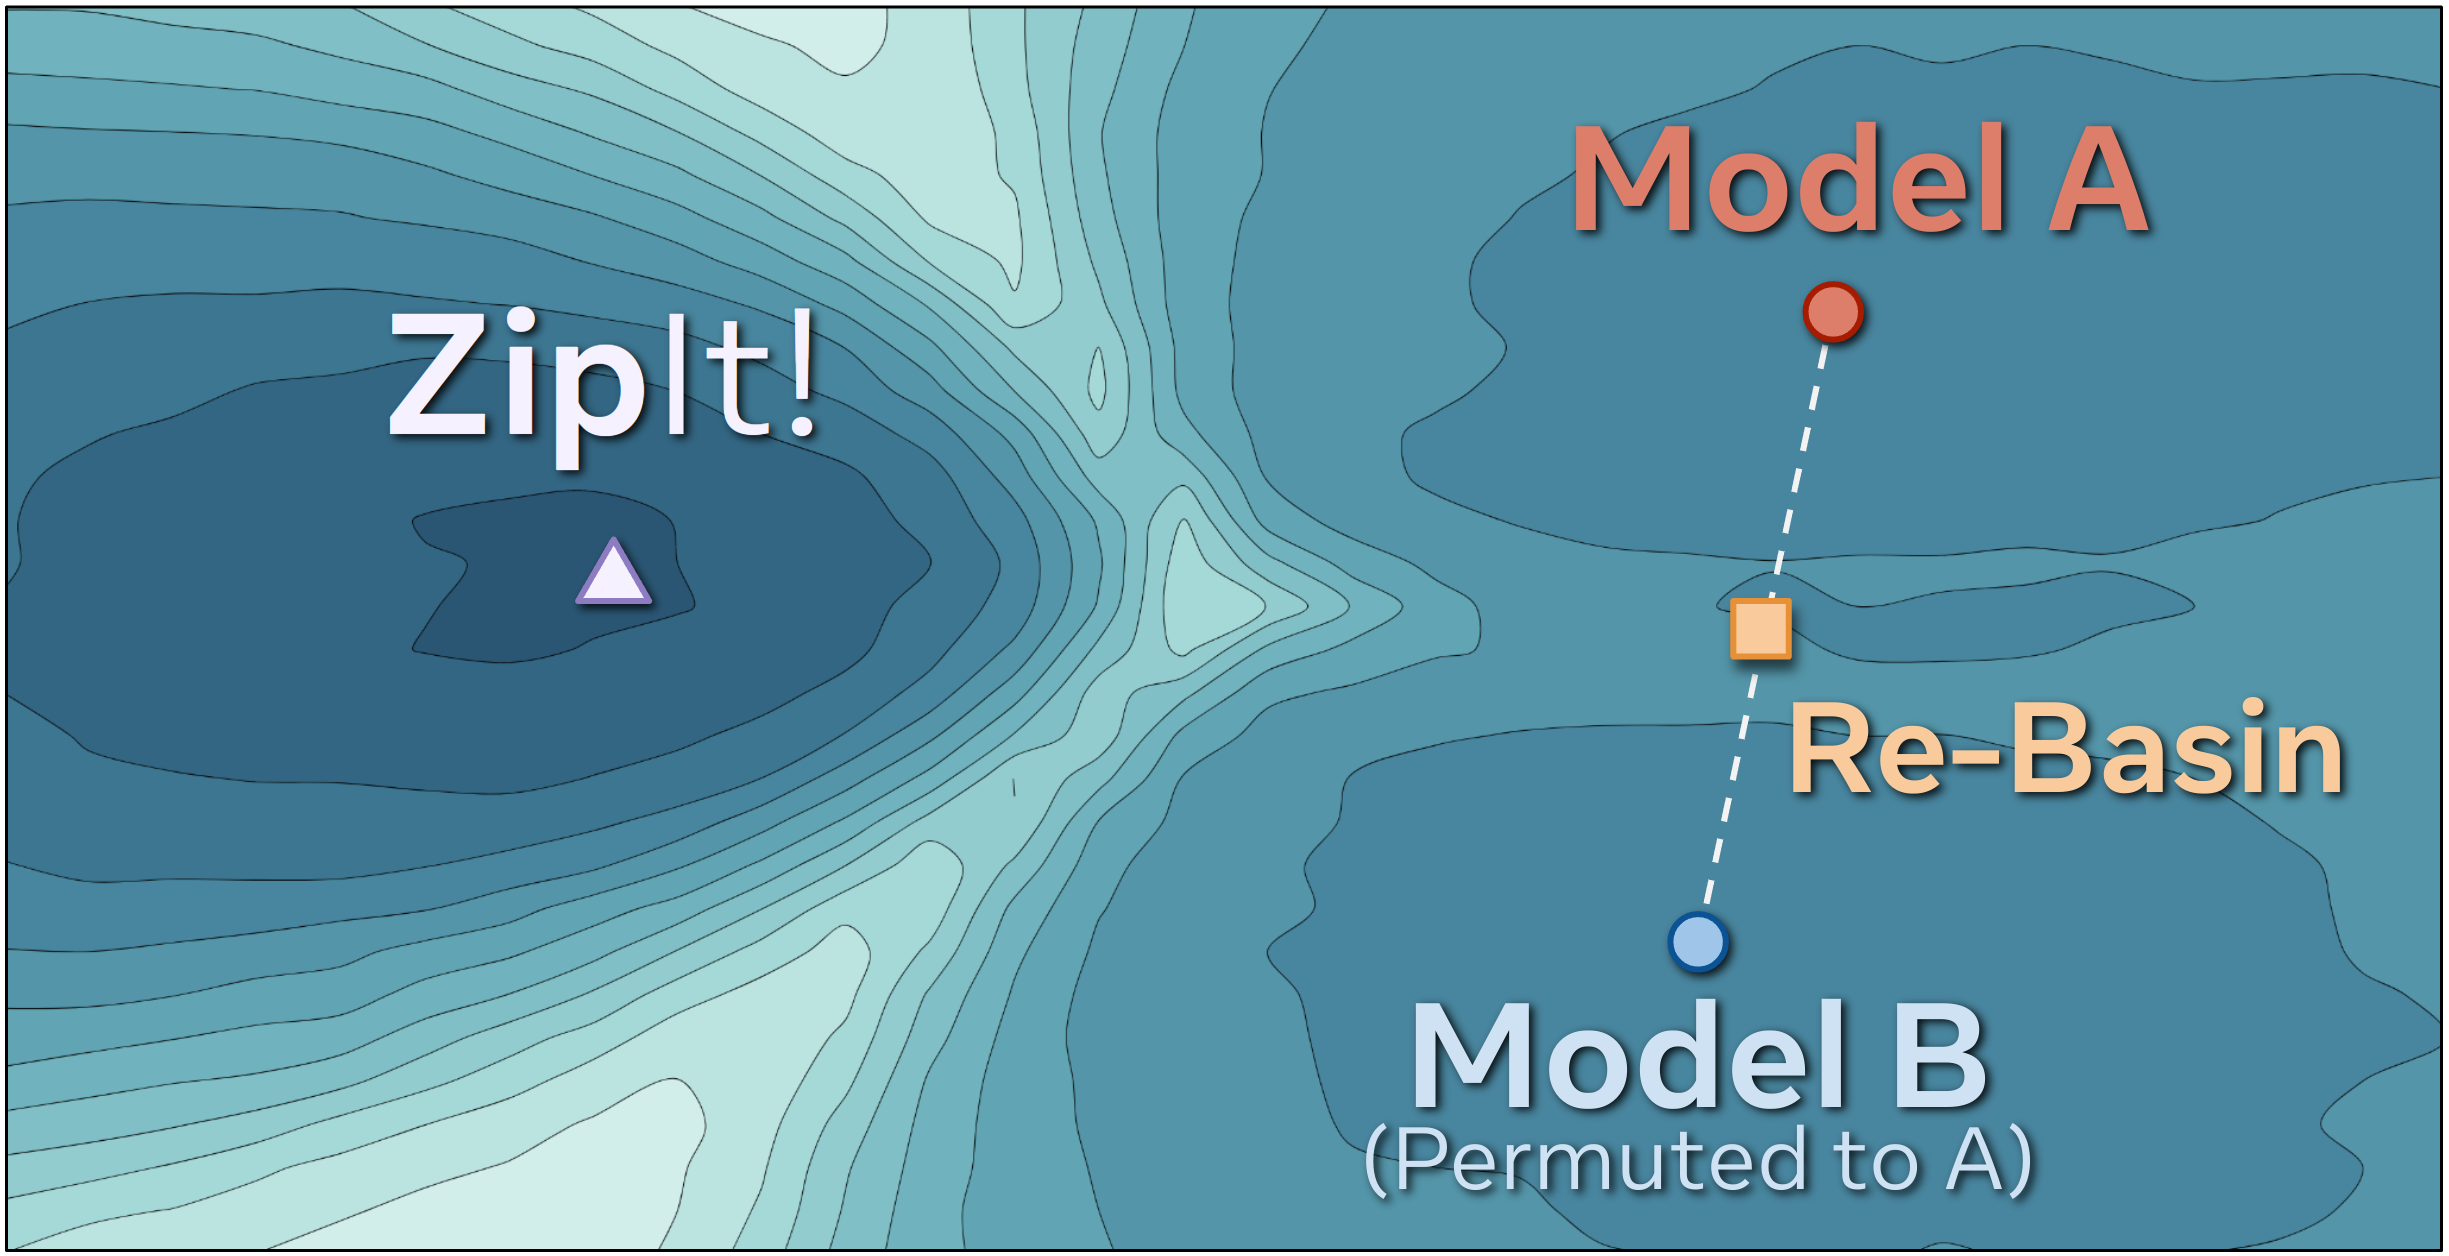
\includegraphics[width=\linewidth]{figures/imgs/loss_basin.png}
%   \newline
%   \caption{{\bf Prior Work Fails} on merging models trained on \textit{different} tasks. Git Re-Basin \cite{ainsworth2022git} assumes the two models lie in the same loss basin \textit{modulo permutation} and interpolates between them. However, that is not sufficient when the models are trained on \textit{different} tasks, here shown for disjoint class sets of CIFAR-100. While \modela{A} and the permuted \modelb{B} lie in similar basins, Git Re-Basin's interpolation performs \textit{worse} than the originals. In contrast, our method \name\ merges them into an even better model in a completely different loss basin.}
%   \label{fig:loss_basin}
%   \vspace{-50pt}
% \end{wrapfigure}



\begin{figure}
  \centering
  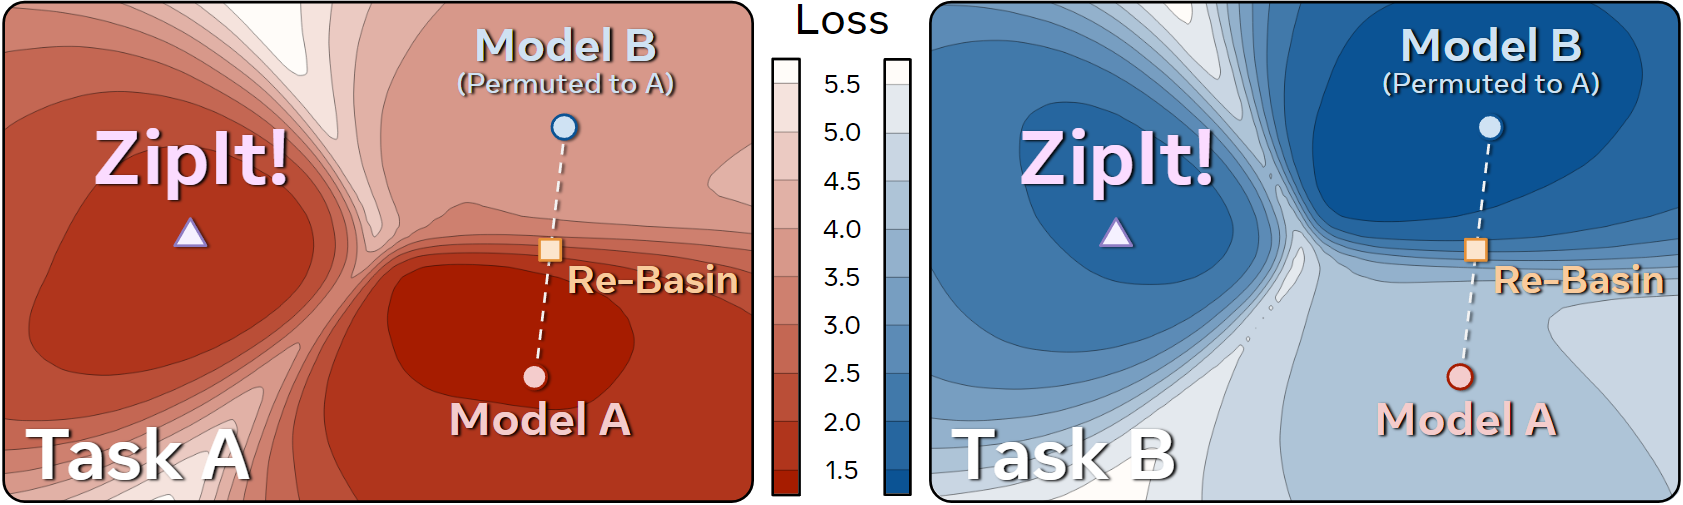
\includegraphics[width=\linewidth]{figures/imgs/loss_landscapes.png}
  % \newline
  % \vspace{-0.5em}
  \caption{{\bf Task Loss Landscapes} for models in Tab.~\ref{tab:cifar50+50}. % Prior work fails on merging models trained on different tasks: 
  \modela{Model A} and \modelb{Model B} lie in low loss basins for their own tasks, but \textit{not for the other task}.
  % While \modelb{Model B} lies in a low loss basin for \modelb{Task B}, it doesn't for \modela{Task A}, even after permuting it to \modela{Model A}.
  % because permuted models for \modela{Task A} likely \textit{do not} lie in a low loss basin for \modelb{Task B}.
  Thus, any interpolation between \modela{Model A} and a permuted \modelb{Model B} (e.g., Git Re-basin) lies outside the minima \textit{for both tasks} and thus performs poorly. In contrast, \name{}\ improves the merge by finding a model that lies in a low loss basin for both.
  % by finding a loss basin common to both tasks.
  % Git Re-Basin~\citet{ainsworth2022git} assumes the two models likely lie in the same loss basin \textit{modulo permutation} and interpolates between them. However, this is substantially less likely when the models are trained on \textit{different} tasks, here shown for disjoint class sets of CIFAR-100. While \modela{A} and \modelb{B} lie in basins on their respective tasks, these \textit{are not} shared across tasks. Thus, Git Re-Basin's interpolation performs \textit{worse} than the original's. In contrast, our method \name{}\ significantly improves the merge by finding a basin common to both tasks. 
  }
  \label{fig:loss_basin}
\end{figure}
\paragraph{Problems with Permutation.}
Eq.~\ref{eq:rebasin} relies on the likelihood of \modelb{model B} lying in the same basin as \modela{model A} after permutation being high. However, this is far less likely when the models are trained on different tasks, as each model optimizes for basins containing distinct task-specific information. In this case the optimal permutation of \modelb{model B} to \modela{model A} still lies in a strong basin on \modelb{task B} but \textit{doesn't} lie in a basin on \modela{task A}, as shown in Figure~\ref{fig:loss_basin}. This causes the interpolated model to perform worse than either the two original models. Thus, we explore alternative merging methods.
% As we show in Figure~\ref{fig:loss_basin}

% While Eq.~\ref{eq:rebasin} works decently well for models trained on the same task, its underlying assumptions break down when the models are trained on \textit{different} tasks. As we show in Fig.~\ref{fig:loss_basin}, these models may not lie in the same loss basin after permutation. In this case, \modelb{Model B}'s optimal permutation lies in a \textit{similar} yet distinct basin to \modela{Model A}. Because the two models are actually in \textit{different basins}, the interpolated result actually has a \textit{lower} accuracy than either of the two original models. This motivates us to explore alternative methods for merging.


% The idea of permutation-based model merging (e.g. Git Re-Basin \cite{ainsworth2022git}) stems from mode connectivity \cite{entezari2021role}, where it has been conjectured that models with different initializations trained on the same data lie in the same \textit{loss basin} (i.e., region of low loss or high accuracy) modulo permutation (as most neural networks can be permuted internally without affecting their outputs). As we show in Fig.~\ref{fig:loss_basin}, this does not hold in our setting where the two models are trained on different tasks. In this case, \modelb{Model B}'s optimal permutation lies in a \textit{similar} yet distinct basin to \modela{Model A}. Because the two models are actually in \textit{different basins}, the interpolated result actually has a \textit{lower} accuracy than either of the two original models. This motivates us to explore alternative methods for merging.

% \subsection{Contributions}
% In addition to extending the problem of model merging to multiple tasks, we further motivate our two primary contributions. 
% Permutation methods focus on exactly mapping every feature in \modela{Model A} to \modelb{Model B} when merging them. 
% This inherently assumes that features across the models are similar, and more likely occurs when the models are trained on the same dataset. 
% However, the likelihood is much smaller when models are trained on different tasks, because their features become less correlated over the course of the network \citep{kornblith2019similarity}. 
% In this case\footnote{unless very rare conditions hold --- please see Appendix~\ref{appendix:postulate2_footnote}}, no permutation may exist to merge the models. 
% Instead, these divergent features between models should be processed via a method other than permutation.

% \paragraph{Merging Within Models.} 
% One way to address this problem is to exploit feature similarity \textit{within} \modela{Model A} and allows these features to be combined with others in \modela{Model A}, while permuting those similar \modelb{Model B} together.
% More specifically, this extends model merging by merging any combination of similar features \textit{within} models, and \textit{across} them.
% Notably, this supports many-1 and many-none in addition to 1-1 merging.
% First, it supports many-to-1 matching because any similar features within \modela{Model A} can be combined together before being permuted to their similar counterpart in \modelb{Model B}, and vice-versa.
% Second, it supports many-to-none matching because the same combined features may instead by matched to any empty feature in \modelb{Model B} obtained when its own features are merged.
% % \name{} demonstrates the efficacy of \name{} through extensive empirical results---improving accuracy by up to \textbf{20\%} over permutation methods---and we further \textit{prove} its approach is \textbf{strictly} better than permutation methods under certain conditions---Appendix~\ref{appendix:postulate}. 

% \paragraph{Partial Merging.} 
% A second way to address this problem is to simply only merge \modela{Model A} and \modelb{Model B} up to layers whose features are non-divergent.
% The intermediate outputs can then be passed into the unmerged layers in \modela{Model A} and \modelb{Model B} to create a multi-head model. 
% While this solution may increase the overall flop count compared to fully merging the models, it can significantly improve performance. 
% % Notably, \name{} outperforms fully merged models by \textbf{over 15\%} while still keeping most layers merged. 




% \paragraph{Permutation Limitations.}
% Models trained on the same task only need to be reasonably sized for permutation based methods to achieve decent performance because they quickly learn redundant features. This is not necessarily true when the models are trained on different tasks, and we consistently find that Eq.~\ref{eq:rebasin} requires \textit{significantly larger} sized models to achieve comparable merging performance (E.g., Figure~\ref{fig:model_size}). However, we find that better merging can be achieved with dramatically lower model size if feature redundancy within models can also be exploited. This is because rather than forcibly merging non-redundant features between models, these can instead be merged with their redundant counterparts in the model. Thus, we make the following conjecture: 
% \begin{center}
%     \textit{Methods that jointly exploit feature redundancy within and across the models are significantly more interpolatable than permutation based approaches, even for dramatically lower model sizes.}
% \end{center}
% The above conjecture is an extension of that from \cite{entezari2021role} and specifies that a lower model size is needed. This is illustrated by Figure~\ref{fig:loss_basin}. We provide both theoretical and empirical evidence in support of this conjecture. Postulate A (Please see Appendix ?) shows its validity in a certain limited setting, driving observations supporting the conjecture found through extensive experimentation.

\section{\name{}} \label{sec:approach}
In this work, we treat model merging as combining the checkpoints (i.e., collection of weights) of multiple models into a single checkpoint that can perform all the tasks of its constituents. 
We do this by merging the layers of the models together.
For instance, suppose $L_i\in\mathcal{L}$ is a linear layer with parameters $W_i \in \mathbb{R}^{n_i\times m_i}, b_i \in \mathbb{R}^{n_i}$ with input features $x \in \mathbb{R}^{m_i}$ and outputs features $f_i \in \mathbb{R}^{n_i}$:
% For instance, if layer $L_i \in \mathcal{L}$ is a linear layer, it has parameters $W_i \in \mathbb{R}^{n_i\times m_i}, b_i \in \mathbb{R}^{n_i}$ and takes input $x \in \mathbb{R}^{m_i}$, with an output feature vector $f_i \in \mathbb{R}^{n_i}$ where
\begin{equation}\label{eq:linear_features}
    f_i = L_i(x) = W_i x + b_i
\end{equation}
Our goal is to take $\modela{L_i^A} \in \modela{\mathcal{L}^A}$ from \modela{model A} and $\modelb{L_i^B} \in \modelb{\mathcal{L}^B}$ from \modelb{model B} and merge them into a layer
% \footnote{Note that we consider activation and normalization to be distinct layers in the network as they are implemented in practice, rather than one combined unit.}
\modelc{$L_i^*$} that combines their feature spaces such that information from both \modela{$f_i^A$} and \modelb{$f_i^B$} is retained in \modelc{$f_i^*$}.
We accomplish this by merging each layer of one model with the corresponding layer in the other, both merging features in one \textit{across} both layers or \textit{within} the same layer.
% both \textit{within} and \textit{across} the layers: We merge each feature in one layer either to another feature either within the layer or across to another feature in the other layer. 
This is in contrast to permutation-based merging method, which only combine features \textit{across} layers.
% This is in-contrast to permutation-based merging, which only merges \textit{across} layers.
% We accomplish this by merging each layer of one model with the corresponding layer in the other, \textit{while modifying both} (in contrast to permutation-based merging, which only permutes one of the models).

\paragraph{Why should we merge \textit{within}?} % Because they solve different problems, features of models trained on different tasks may be dissimilar.
Features of models trained on different tasks may be dissimilar, as the models solve different problems. 
Forcibly combining these dissimilar features can yield merges that don't perform well on either original task (Fig~\ref{fig:loss_basin}).
Instead, those features may be more compatible with others within the same model, which would better retain performance when combined. % allowing them to be combined while retaining performance.
% These can be combined together and retain task capability.
% This can cause poor merges if they're combined with each other across the models. 
% However, these same features may be more similar (or redundant) to others \textit{within} the same model, making those better fits for merging.

In fact, we can \textit{prove} that methods which allow merges \textit{within} each model (as well as across both) perform equal to or \textit{better} than those which only merge across models (e.g., permutation-reliant approaches) in a limited but prevalent setting.
Specifically, we obtain a tighter bound over Theorem 3.1 from \citet{entezari2021role} when redundancy exists within a model and is leveraged. 
Both Theorem 3.1 and our Theorem \hyperref[ap:TheoremDef]{1} (see Appendix~\ref{ap:Theorem} for formalization and proof) bound the degree to which the loss of a merged two-layer model with $d$-input dimensions and $h$-intermediate dimensions increases compared to the losses of the original models. 
Theorem 3.1 bounds this increase to $\Tilde{O}(h^{-\sfrac{1}{(2d+4)}})$.
However, if features within a model are \textit{redundant}, then we reduce the bound to%
% (with $\Gamma\in[0,1]$ measuring what portion of features are redundant), then we substantially reduce the bound to
%is taken into account, then we substantially reduce the bound to,
%($0$ means nothing is similar and $1$ means everything is similar)
\begin{equation} \label{eq:mainpaper_barrier}
    \text{Loss Increase of Merged Model} \leq
        \begin{cases}
            \Tilde{O}\left(\left(\frac{h}{1-2\Gamma}\right)^{-\frac{1}{2d+4}}  \right) & \Gamma < 0.5 \\
            0 &\text{otherwise}
        \end{cases}
\end{equation}
with $\Gamma\in[0,1]$ measuring what portion of features are redundant. 
% This bound is 
This bound is %$\sqrt[2d+4]{1-2\Gamma} \leq 1$
$\sqrt[2d+4]{1-2\Gamma} \leq 1$
times that of Theorem 3.1 when $\Gamma < 0.5$ (equal only when $\Gamma = 0$) and \textit{explicitly zero} when $\Gamma \geq 0.5$.
% and is
% strictly less than Theorem 3.1 when $\Gamma\in(0,1]$ (achieving \textit{zero no matter $h$} when $\Gamma \geq 0.5$), and is only equal at $\Gamma=0$. 

% Prior work only modifies a single model \citep{ainsworth2022git,entezari2021role}. 
% These assume that features in one model have a similar counterpart in the second, and thus can be permuted from one model to match the second.
% However, the features of models trained on different tasks may be dissimilar because they solve different problems.
% In this case, no permutations may exist to match the two models.
% Instead, these features may be more similar (or redundant) to others in the same model and thus should be combined with those \textit{within} a model rather than \textit{across} models.

% We justify this intuition by \textbf{proving} that methods which exploit this phenomenon when it exists are \textit{strictly} better than permutation-reliant approaches in a limited but prevalent setting.
% Specifically, we obtain a significantly tighter bound over Theorem 3.1 from \citet{entezari2021role} in the same setting when similarity within a model exists and is leveraged.
% Theorem 3.1 bounds the degree to which permutations degrade the loss of a merged two-layer model with $d$-input dimensions and $h$-intermediate dimensions to $\Tilde{O}(h^{-\frac{1}{2d+4}})$.
% However, if we let $\Gamma$ denote the proportion of similar features within each model where $\Gamma\in[0,1]$, such that $\Gamma=0$ indicates nothing is similar and $\Gamma=1$ means everything is similar, we can leverage properties from \citet{simsek2021geometry} to obtain the tighter piece-wise bound:
% \begin{equation*}
%     \text{Loss Increase of Merged Model} \leq
%         \begin{cases}
%             \Tilde{O}\left(\left(\frac{h}{1-2\Gamma}\right)^{-\frac{1}{2d+4}}  \right) & \Gamma > 0.5 \\
%             0 &\text{otherwise}
%         \end{cases}
% \end{equation*}
% This bound is strictly lower than Theorem 3.1 when $\Gamma\in(0,1]$ with equality at $\Gamma=0$. 
% Also, unlike Theorem 3.1, it achieves zero-bound regardless of the intermediate dimension size when models have sufficient internal feature similarities. 
% Due to space restrictions, we leave further details and the proof to Appendix~\ref{ap:Theorem}.

% Please see Appendix~\ref{ap:Theorem} for more details. 

% In this work, we treat model merging as jointly combining the checkpoints (i.e., collection of weights) of two models into a single checkpoint that can perform all the tasks of its constituents.
% This is done by first transforming (e.g., prior work uses permutation) their and then interpolating between these new features in each model. 

% Models trained on different tasks solve different problems, causing their features to be more dissimilar.
% In this case, no permutation may exist to merge the models because some features in one model will not be similar to any in the second. 

% The features of models trained on different tasks 
% In this case, no permutation of features may

% When models are trained on different tasks, their features are far less likely to be similar 


% When models are trained on different tasks, their features become less correlated over the course of the network \citep{kornblith2019similarity}. 

% The features of models trained on different tasks become less correlated over the course of the network \citet{kornblith2019similarity}.
% In this case, no permutation of features may exist to merge the models and thus may permutation-based merging methods to fail.
% Instead, these divergent features between models should be processed via a method other than permutation.
% This makes permutation-based merging methods, which exactly map all features in one model to the other, substantially less likely to succeed.



% Permutation methods exactly map every feature in \modela{Model A} to \modelb{Model B} when merging them. 
% This inherently assumes that features across the models are similar, and more likely occurs when the models are trained on the same dataset. 
% However, the likelihood is much smaller when models are trained on different tasks, because their features become less correlated over the course of the network \citep{kornblith2019similarity}. 
% In this case\footnote{unless very rare conditions hold --- please see Appendix~\ref{ap:Theorem2_footnote}}, no permutation may exist to merge the models. 
% Instead, these divergent features between models should be processed via a method other than permutation.

% \paragraph{Merging Within Models.} 
% One way to address this problem is to exploit feature similarity \textit{within} \modela{Model A} and allows these features to be combined with others in \modela{Model A}, while permuting those similar \modelb{Model B} together.
% More specifically, this extends model merging by merging any combination of similar features \textit{within} models, and \textit{across} them.
% Notably, this supports many-1 and many-none in addition to 1-1 merging.
% First, it supports many-to-1 matching because any similar features within \modela{Model A} can be combined together before being permuted to their similar counterpart in \modelb{Model B}, and vice-versa.
% Second, it supports many-to-none matching because the same combined features may instead by matched to any empty feature in \modelb{Model B} obtained when its own features are merged.
% \name{} demonstrates the efficacy of \name{} through extensive empirical results---improving accuracy by up to \textbf{20\%} over permutation methods---and we further \textit{prove} its approach is \textbf{strictly} better than permutation methods under certain conditions---Appendix~\ref{ap:Theorem}. 

% In this work, we treat model merging as jointly combining the checkpoints (i.e., collection of weights) of two models into a single checkpoint that can perform all the tasks of its constituents. We accomplish this by merging each layer of one model with the corresponding layer in the other, \textit{while modifying both} (in contrast to permutation-based merging, which only permutes one of the models).

% For instance, if layer $L_i \in \mathcal{L}$ is a linear layer, it has parameters $W_i \in \mathbb{R}^{n_i\times m_i}, b_i \in \mathbb{R}^{n_i}$ and takes input $x \in \mathbb{R}^{m_i}$, with an output feature vector $f_i \in \mathbb{R}^{n_i}$ where
% \begin{equation}\label{eq:linear_features}
%     f_i = L_i(x) = W_i x + b_i
% \end{equation}
% Then our goal is to take $\modela{L_i^A} \in \modela{\mathcal{L}^A}$ from \modela{model A} and $\modelb{L_i^B} \in \modelb{\mathcal{L}^B}$ from \modelb{model B} and merge them into a layer \modelc{$L_i^*$} that combines their feature spaces such that information from both \modela{$f_i^A$} and \modelb{$f_i^B$} is retained in \modelc{$f_i^*$}.
% Note that we consider activation and normalization to be distinct layers in the network as they are implemented in practice, rather than one combined unit.



\paragraph{How do we merge features?}
% \paragraph{How do we obtain the combined features \modelc{$f_i^*$}?}
In prior work, each of the merged features \modelc{$f_i^*$} is the result of combining one feature from \modela{$f_i^A$} and one from \modelb{$f_i^B$}. 
However in our case, we can also merge features by combining two from just \modela{$f_i^A$} or two from just \modelb{$f_i^B$}. To account for this, we concatenate \modela{$f_i^A$} and \modelb{$f_i^B$} into a single feature vector:  $\modela{f_i^A}\|\modelb{f_i^B} \in \mathbb{R}^{2n_i}$. Then, like prior work (e.g. \citet{li2016convergenticlr,jordan2022repair}), we define feature similarity as the pairwise correlation between between neuron activations over a small set of images (without labels). However, unlike those works, we compute correlations between every activation in \textit{the full concatenated space} $\modela{f_i^A}\|\modelb{f_i^B}$. Our approach thus measures the similarity of every feature $\modela{f_i^A}$ and $\modelb{f_i^B}$ to all features in both models, rather than solely between $\modela{f_i^A}$ and $\modelb{f_i^B}$.
% If two features are very similar,
% then we can interpolate them without losing much information.
% These features can either be in $\modela{f_i^A}$ and $\modelb{f_i^B}$ (\textit{across} layers), or be in just $\modela{f_i^A}$ or $\modelb{f_i^B}$ (\textit{within} a layer).

% unlike permutation-based approaches (e.g. \citet{li2016convergenticlr,jordan2022repair}), we compute pairwise correlations between every neuron activation in \textit{the full concatenated space} $\modela{f_i^A}\|\modelb{f_i^B}$ over a small set of images (without labels).

Next, if two features are well correlated, we can average them without losing much information. Thus, we can construct \modelc{$f_i^*$} by finding $n_i$ pairs of similar features in $\modela{f_i^A}\|\modelb{f_i^B}$ and averaging them together. By default, we do this greedily: i.e., iteratively match the features with the highest correlation without replacement; though we explore extensions to this in Sec.~\ref{sec:extensions} and test other methods in Tab.~\ref{tab:matching_alg}. Then we can use these matches to construct \modelc{$f_i^*$}. Formally, we define a ``merge matrix'' $\modelc{M_i} \in \mathbb{R}^{n_i\times2n_i}$ s.t.
\begin{equation}
    \modelc{f_i^*} = \modelc{M_i}\left(\modela{f_i^A}\|\modelb{f_i^B}\right)
\end{equation}
$\modelc{M_i}$ averages the matched features, with each match corresponding to one output feature in $\modelc{f_i^*}$. For instance, if $u$th match is between indices $s, t \in \{1, \ldots, 2n_i\}$ of $\modela{f_i^A}\|\modelb{f_i^B}$, then the $u$th row of $\modelc{M_i}$ would be $\sfrac{1}{2}$ at columns $s$ and $t$ and 0 elsewhere. This results in $\modelc{f_i^*}[u] = \frac{1}{2} (\modela{f_i^A}\|\modelb{f_i^B})[s] + \frac{1}{2} (\modela{f_i^A}\|\modelb{f_i^B})[t]$.
Thus, applying $\modelc{M_i}$ has the effect of interpolating with $\gamma=\sfrac{1}{2}$ but is more general (e.g., allows for merging more than 2 models at once, see Sec.~\ref{sec:extensions}).

% We achieve this by first computing the pairwise correlations between every neuron activation in both \modela{$f_i^A$} and \modelb{$f_i^B$} over a label-less set of data.
% This differs from \citet{li2016convergenticlr,ainsworth2022git, entezari2021role, jordan2022repair} which instead only measure the pairwise correlation of neuron activations in $\modelb{f_i^B}$ to those in $\modela{f_i^A}$.
% As in prior work, we then define the similarity between any two features to simply be the correlation of the neuron activations from each.
% Notably, this means that our approach has the effect of measuring the similarity of every feature in either $\modela{f_i^A}$ and $\modelb{f_i^B}$ to all features in both models, rather than solely between $\modela{f_i^A}$ and $\modelb{f_i^B}$ as in prior work.

% We achieve this by first concatenating the feature vectors \modela{$f_i^A$} and \modelb{$f_i^B$} together into a vector:  $\modela{f_i^A}\|\modelb{f_i^B} \in \mathbb{R}^{2n_i}$.
% We then calculate the pairwise correlations of every feature in $\modela{f_i^A}\|\modelb{f_i^B}$ with every other feature in the vector---following the strategy of \citep{li2016convergenticlr}.
% This has the effect of measuring the correlation of every feature in either $\modela{f_i^A}$ and $\modelb{f_i^B}$ to all features in both models.
% Note, this differs from \citet{li2016convergenticlr,ainsworth2022git, entezari2021role, jordan2022repair} which instead only measure the correlation of features in $\modelb{f_i^B}$ to those in $\modela{f_i^A}$.
% If two features are highly correlated, 
% If two features are very similar,
% then we can interpolate them without losing much information.
% These features can either be in $\modela{f_i^A}$ and $\modelb{f_i^B}$ (\textit{across} layers), or be in just $\modela{f_i^A}$ or $\modelb{f_i^B}$ (\textit{within} a layer).

% \textcolor{red}{
% Thus, if we can find a good pairing for each element in both $\modela{f_i^A}$ and $\modelb{f_i^B}$ (leaving us with $n_i$ pairs), we can construct a merged feature \modelc{$f_i^*$} that contains an efficiently compressed representation of $\modela{f_i^A}$ and $\modelb{f_i^B}$ by averaging each pair of features. 
% This is equivalent to interpolating with $\gamma=\sfrac{1}{2}$.
% In practice we apply this merge in two steps. First, we concatenate the feature vectors \modela{$f_i^A$} and \modelb{$f_i^B$} together into a vector:  $\modela{f_i^A}\|\modelb{f_i^B} \in \mathbb{R}^{2n_i}$.
% Second, we define a ``merge matrix'' $\modelc{M_i} \in \mathbb{R}^{n_i\times2n_i}$ such that
% }
% Thus, if we can find a good pairing for each element of the concatenated $\modela{f_i^A}\|\modelb{f_i^B}$ (leaving us with $n_i$ pairs), we can construct a merged feature \modelc{$f_i^*$} that contains an efficiently compressed representation of $\modela{f_i^A}$ and $\modelb{f_i^B}$ by 
% averaging each pair of features. 
% \textcolor{red}{This is equivalent to interpolating with $\gamma=\sfrac{1}{2}$.}
% % \textcolor{red}{interpolating each pair of features}.
% In practice, we apply this merge by defining a ``merge matrix'' $\modelc{M_i} \in \mathbb{R}^{n_i\times2n_i}$ such that
% \begin{equation}
%     \modelc{f_i^*} = \modelc{M_i}\left(\modela{f_i^A}\|\modelb{f_i^B}\right)
% \end{equation}
% % The resulting \modelc{$M_i$} is non-zero (taking a value of $\sfrac{1}{2}$ only at indices corresponding to feature pairs in $\modela{f_i^A}\|\modelb{f_i^B}$ that are merged together.
% The resulting \modelc{$M_i$} is $\sfrac{1}{2}$ for indices corresponding to matched pairs in $\modela{f_i^A}\|\modelb{f_i^B}$ and 0 elsewhere. Thus, \modelc{$M_i$} has the effect of selects paired features from $\modela{f_i^A}\|\modelb{f_i^B}$ and averaging them.
% % is zero everywhere except for each pair with index $p$ of matches $(j, k)$, \modelc{${M_i}_{[p,j]} = {M_i}_{[p,k]} = \sfrac{1}{2}$}. 
% We find these matches greedily---an optimal algorithm exists but is very slow and only slightly more accurate (Tab.~\ref{tab:matching_alg}).


% In order to construct the combined features \modelc{$f_i^*$}, we assume that there are some redundant features in \modela{$f_i^A$} and \modelb{$f_i^B$}. 
% That is, we assume some elements of the two feature vectors are \textit{highly correlated} over a sample of data. 
% \textcolor{blue}{
% We use the same definition of correlation as in \citep{li2016convergenticlr}.
% }
% In this work, we consider correlations between features \textit{within} the same model and \textit{across} the two models. In practice we concatenate the two feature vectors into $\modela{f_i^A}\|\modelb{f_i^B} \in \mathbb{R}^{2n_i}$ and consider correlations between each pair of elements in this concatenated vector, which differs from prior work \cite{ainsworth2022git,jordan2022repair} that only consider correlations \textit{across} the two models.

% If two features are highly correlated, then we can average them without losing much information.
% Thus, if we can find a good pairing for each element of the concatenated $\modela{f_i^A}\|\modelb{f_i^B}$ (leaving us with $n_i$ pairs), we can construct a merged feature \modelc{$f_i^*$} that contains an efficiently compressed representation of $\modela{f_i^A}$ and $\modelb{f_i^B}$ by averaging each pair of features. In practice, we define a merge matrix $\modelc{M_i} \in \mathbb{R}^{n_i\times2n_i}$ s.t.
% \begin{equation}
%     \modelc{f_i^*} = \modelc{M_i}\left(\modela{f_i^A}\|\modelb{f_i^B}\right)
% \end{equation}
% The resulting \modelc{$M_i$} is zero everywhere except for each pair with index $p$ of matches $(j, k)$, \modelc{${M_i}_{[p,j]} = {M_i}_{[p,k]} = \sfrac{1}{2}$}. We find these matches greedily---an optimal algorithm exists but is very slow and only slightly more accurate (Tab.~\ref{tab:matching_alg}).


\paragraph{What about the next layer?}
After merging features in one layer, we now have the problem that the next layers, $\modela{L_{i+1}^A}, \modelb{L_{i+1}^B}$, are incompatible with $\modelc{f_i^*}$. Instead, we need to \textit{undo} the merge operation before passing the features to the next layer. Thus, we define an ``unmerge'' matrix $\modelc{U_i} \in \mathbb{R}^{2n_i \times n_i}$ s.t.
\begin{equation}
    \modelc{U_i f_i^*} \approx \modela{f_i^A}\|\modelb{f_i^B}
\end{equation}
$\modelc{U_i}$ is the pseudoinverse of $M_i$ and in the case of the matching from earlier is simply $2\modelc{M_i}^T$.
% In the case of the matching from earlier, $\modelc{U_i}$ has the effect of ``copying'' the merged features back to their original locations and is simply $2\modelc{M_i}^T$ (with $2\times$ to cancel out the $\sfrac{1}{2}$ from averaging).
% In the case of the matching from earlier, $\modelc{U_i}$ is simply $2\modelc{M_i}^T$ and has the effect of ``copying'' the merged features back to their original locations. 
%Note that in most cases, we can't have a strict equality here because $\modelc{U_i}$ isn't full rank.
Note that strict equality is unlikely here. Like in prior work, merging models is a lossy operation. % , we can't have a strict equality here because $\modelc{U_i}$ isn't full rank.

We 
% can further 
split this unmerge matrix in half along its rows into $\modela{U_i^A}, \modelb{U_i^B} \in \mathbb{R}^{n_i\times n_i}$ that act individually to produce \modela{$f_i^A$} and \modelb{$f_i^B$}. 
% by splitting \modelc{$U_i$}  in half along its rows. 
With this, we can evaluate the next layers using the merged features:
\begin{equation}
    \modela{f_{i+1}^A} \approx \modela{L_{i+1}^A}(\modela{U_i^A} \modelc{f_i^*}) \qquad \modelb{f_{i+1}^B} \approx \modelb{L_{i+1}^B}(\modelb{U_i^B} \modelc{f_i^*})
\end{equation}



\subsection{The ``Zip'' Operation}
We now have
% Now that we have
all 
the necessary pieces, 
% we 
and can derive a general operation to merge \modela{$L_i^A$} and \modelb{$L_i^B$} at an arbitrary point in the network (Fig.~\ref{fig:zip_op}).
First, we compute \modelc{$M_i$} and \modelc{$U_i$} by matching features between \modela{$f_i^A$} and \modelb{$f_i^B$}. We then pass \modelc{$U_i$} to the next layer and receive \modelc{$U_{i-1}$} from the previous layer. Using \modelc{$M_i$} and \modelc{$U_{i-1}$}, we 
% can now 
``fuse'' the merge and unmerge operations into the layer's parameters. For a linear layer:
\begin{equation} \label{eq:zip}
    % \modelc{W^*_i} = \gamma\modela{M_i^A W_i^A U^A_{i-1}} + (1-\gamma)\modelb{M_i^B W_i^B U^B_{i-1}}
    \modelc{W^*_i} = \modela{M_i^A W_i^A U^A_{i-1}} + \modelb{M_i^B W_i^B U^B_{i-1}}
\end{equation}
where \modela{$M_i^A$} and \modelb{$M_i^B$} are \modelc{$M_i$} split along its columns.
% and $\gamma$ is a hyperparameter we set to $\sfrac{1}{2}$.
\modelc{$b_i^*$} has the same equation but without unmerging.

Note the similarity between Eq.~\ref{eq:zip} and Eq.~\ref{eq:rebasin}. This isn't a coincidence: if we only allowed merging \textit{across} models and not \textit{within} models, our ``zip'' operation would be identical to Git Re-Basin's permute-then-interpolate approach. Thus, Eq.~\ref{eq:zip} can be thought of as a generalization of prior work.


\begin{figure*}
    \centering
    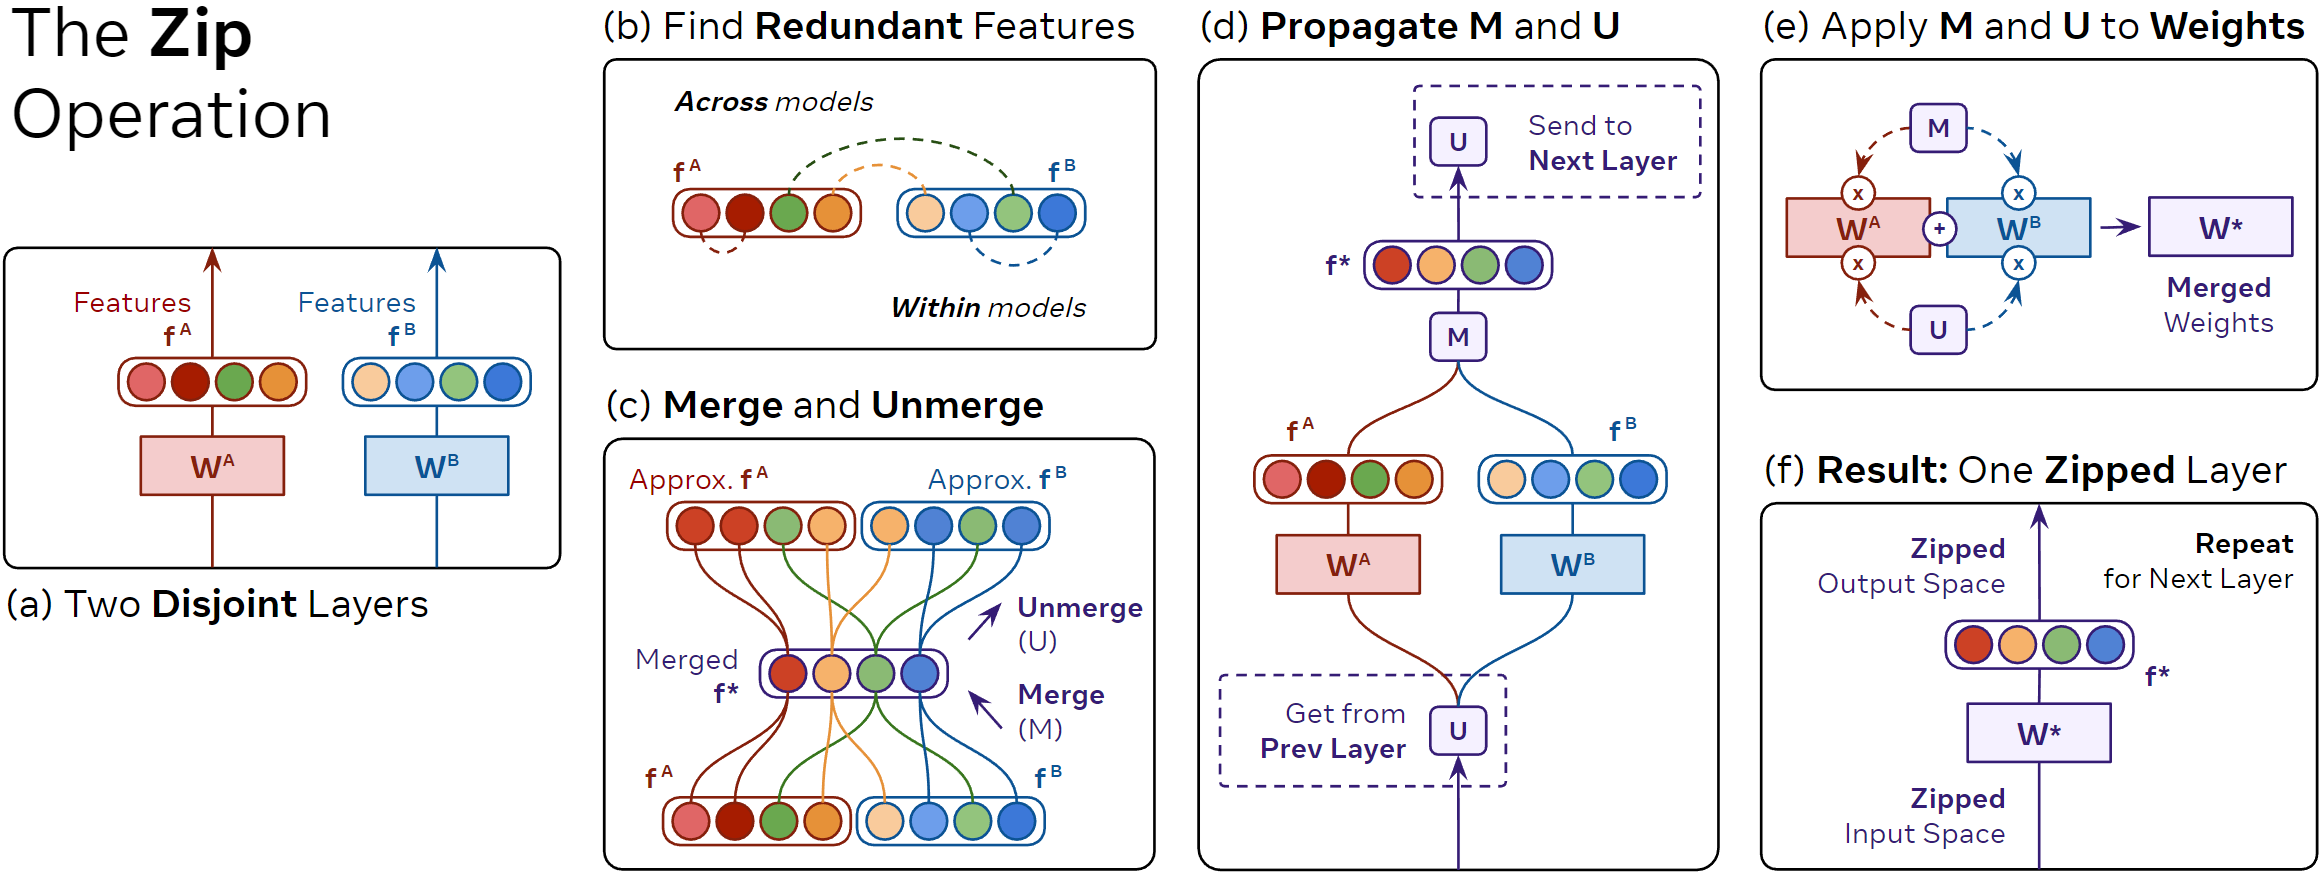
\includegraphics[width=0.95\linewidth]{figures/imgs/zip_it.png}
    \caption{{\bf \name{}} merges models layer-wise by exploiting redundancy in their features. 
    % (a) Starting with completely disjoint layers with weights \modela{$W^{A}$} and \modelb{$W^{B}$} from models trained on different tasks, (b) we match redundant features by comparing their activations \modela{$f^{A}$} and \modelb{$f^{B}$}. (c) We use this matching to produce a merge matrix \modelc{M} to combine \modela{$f^{A}$} and \modelb{$f^{B}$} into a single shared feature space \modelc{$f^{*}$} and a corresponding unmerge matrix \modelc{U} that undoes this operation. (d) In order to align the input space of the next layer, we propagate \modelc{U} forward along network and at the same time receive a \modelc{U} matrix from the previous layer. (e) Once we have both an \modelc{M} for the output, and a \modelc{U} for the input, we can ``zip'' the layers together by applying Eq.~\ref{eq:zip}. (f) The result is a single layer with a shared input and output space, and we can now repeat from (a) on the next layer.
    (a) Output features \modela{$f^{A}$} and \modelb{$f^{B}$} from two disjoint layers are (b) paired with other features based on the similarity of their activations. (c) We produce a merge matrix \modelc{M} to combine the pairs into a single shared output feature space, and a corresponding unmerge matrix \modelc{U} that undoes this operation. (d) We then propagate \modelc{U} up the network to align the next layer's input space, and simultaneously receive the previous layer's \modelc{U} to align our input space. (e) We apply Eq.~\ref{eq:zip} to ``zip'' the layers together using the \modelc{M} for the output and \modelc{U} for the input, producing a single layer (f). We then repeat (a) on the next layer.
    % . (f) We obtain a single layer with a shared input and output space. We then repeat from (a) on the next layer. 
    }
    \label{fig:zip_op}
\end{figure*}
\begin{figure}[t]
\centering

\begin{minipage}{0.48\linewidth}{
    \centering
    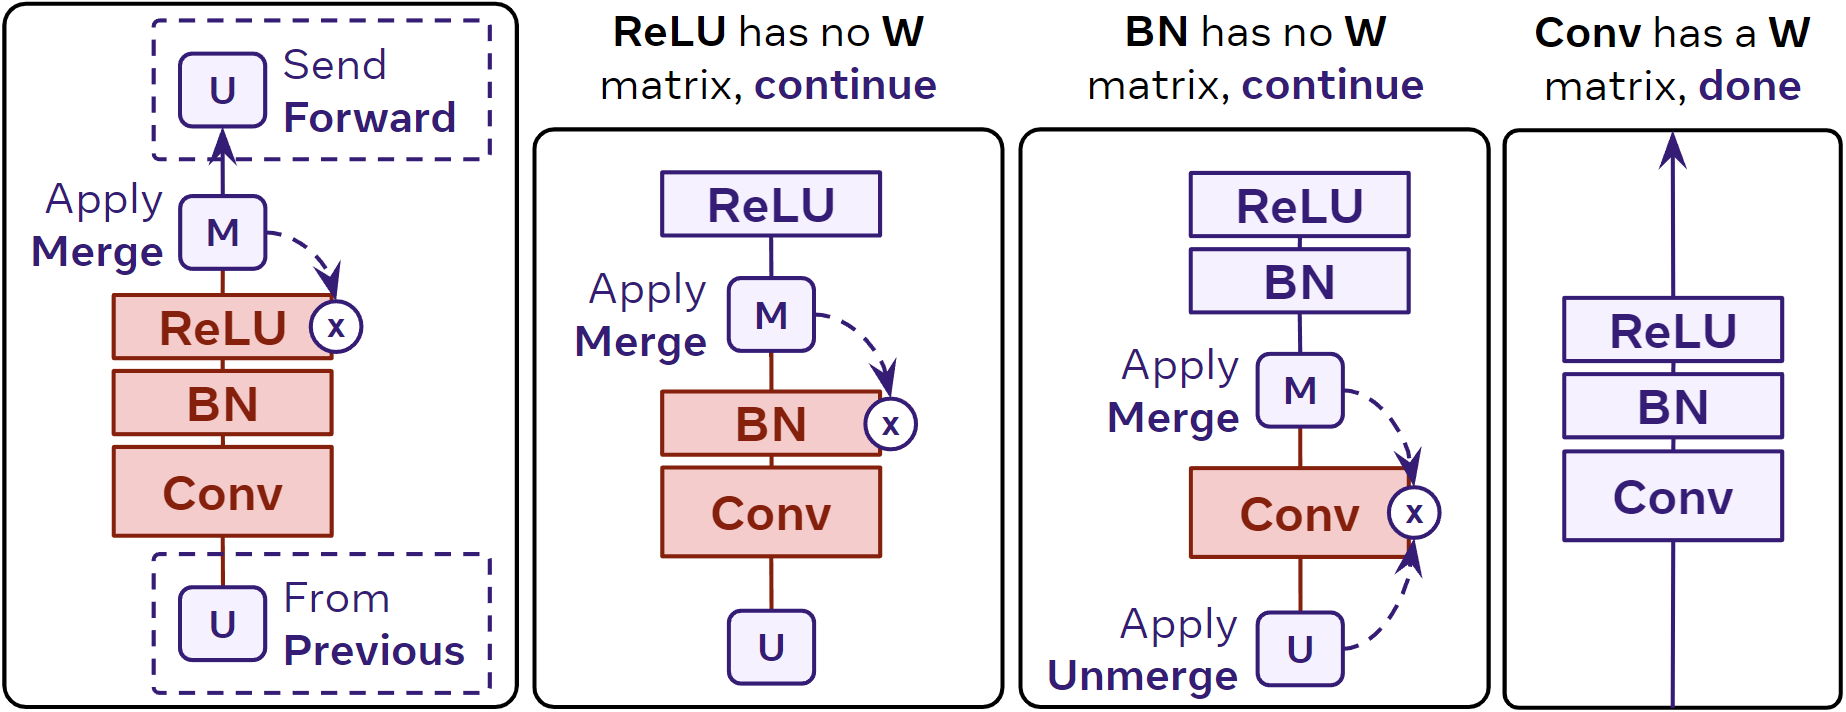
\includegraphics[width=\linewidth]{figures/imgs/zip_prop.png}
    \caption{{\bf Zip Propagation.} 
    % In practice, we compute \modelc{$M_i$} and \modelc{$U_i$} after activations (e.g., ReLU). 
    We propagate \modelc{$M_i$} backward until we hit a layer with weights, merging merging element-wise layers (e.g., BatchNorm) along the way.
    % We can't apply Eq.~\ref{eq:zip} to a layer without a weight matrix and have to propagate \modelc{$M_i$} backward until we hit such a layer. all element-wise layers (e.g., BatchNorm) are merged along the way.
    % Since we can't apply Eq.~\ref{eq:zip} to a layer without a weight matrix, we have to propagate \modelc{$M_i$} backward until we hit such a layer, merging element-wise layers (e.g., BatchNorm) along the way.
    }
    \label{fig:zip_prop}
}\end{minipage}
\hspace{1em}
\begin{minipage}{0.48\linewidth}{
    \centering
    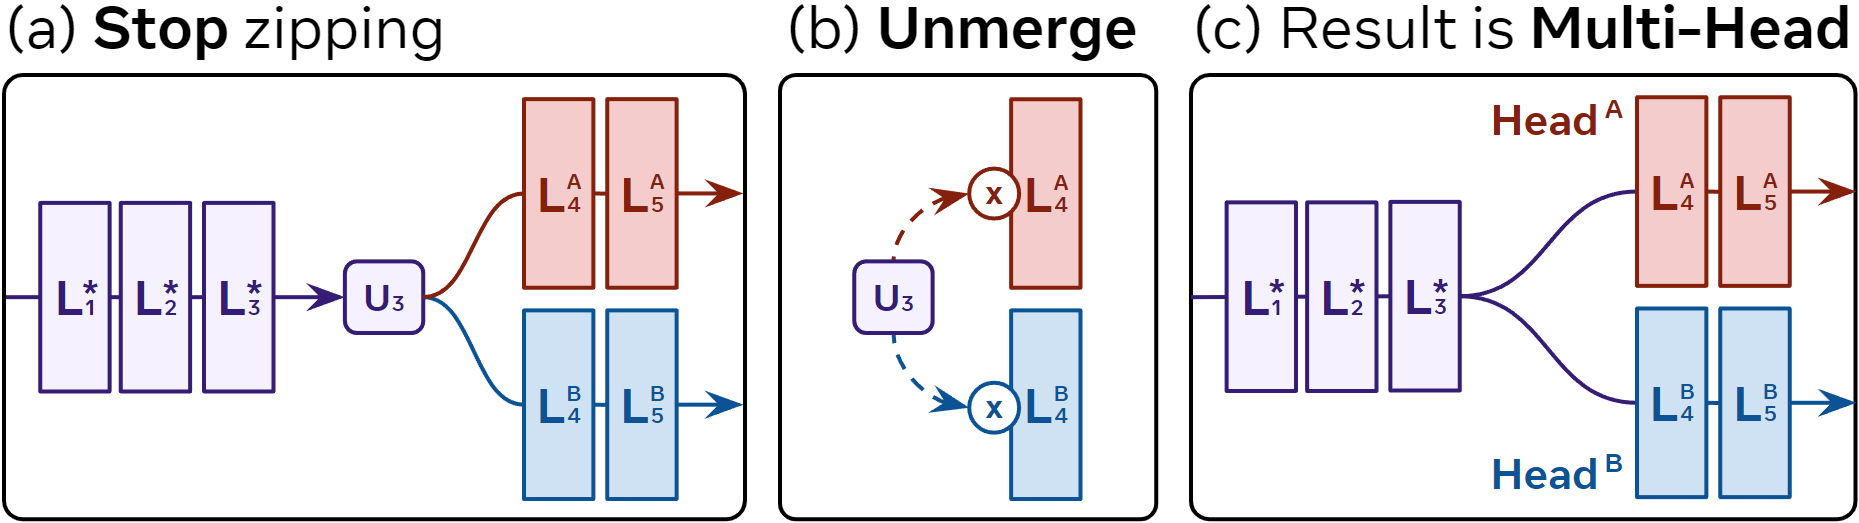
\includegraphics[width=\linewidth]{figures/imgs/partial_zip.png}
    \caption{
        {\bf Partial Zip.}
        (a) If we stop zipping early and (b) apply the latest \modelc{U} from the zip propagation to the inputs of the first unmerged layer in each model, (c) we get a multi-head model with a head for each task.
        % If we stop zipping early (a), we can create a multi-head model that can perform multiple tasks. All we need to do is apply the last unmerge from zip propogation (Fig.~\ref{fig:zip_prop}) to the inputs of the first unmerged layer in each model (b), and we get a model with multiple heads (c).
    }
    \label{fig:partial_zip}
}\end{minipage}
\vspace{-10pt}
\end{figure}

\subsection{Zip Propagation} \label{sec:zip_prop}
However, most modern neural networks are not simply collections of linear layers stacked on top of each other. In practice, we cannot combine merge and unmerge matrices into every layer of the network, as a local zip (Eq.~\ref{eq:zip}) expects the layer to have a weight \textit{matrix}---i.e., the layer has to have separate input and output spaces so that we can unmerge the input space and merge the output space. Other layers (e.g., BatchNorm, ReLU) don't have such a weight matrix.

Thus, we ``propogate'' \modelc{$M_i$} and \modelc{$U_i$} \textit{through} these layers. For instance, in Fig.~\ref{fig:zip_prop}, we show a common stack of layers found in a typical ConvNet. Following \citet{jordan2022repair}, we compute \modelc{$M_i$} and \modelc{$U_i$} using the activations of the network (i.e., after each ReLU). We can't fuse \modelc{$M_i$} with the ReLU layer, as it doesn't have any parameters. Similarly, we can merge the parameters of the preceding BatchNorm layer (i.e., in the same way as bias). But it doesn't have a weight matrix, so we also can't fuse \modelc{$M_i$} into it. Only once we've reached the Conv layer can we fuse \modelc{$M_i$} and \modelc{$U_i$} into it using Eq.~\ref{eq:zip} (in this case, treating each kernel element as independent).

Similar care needs to be taken with skip connections, as every layer that takes input from or outputs to a skip connection shares the same feature space. However, this too can be dealt with during propagation---we just need to propagate \modelc{$M_i$} backward and \modelc{$U_i$} forward to each layer connected by the same skip connection. 
In general, we can define propagation rules to handle many different types of network modules (see Appendix~\ref{ap:prop_rules}).


\subsection{Extensions}\label{sec:extensions}

\paragraph{Partial Zip.} \label{sec:partial_zip}
% In many cases, 
We don't always want to zip every layer of the two networks, especially if their output spaces are incompatible, or if doing so would lose too much accuracy. 
% In those cases, 
Instead, we can perform a \textit{partial zip}. That is, we zip most of the layers together, but leave
% some of 
the later ones \textit{unzipped} (Fig.~\ref{fig:partial_zip}).

Implementing this operation is simple in our framework: zip as normal until the specified layer $i$, then the remaining unzipped layers will receive \modelc{$U_i$} through zip propagation. If we apply \modela{$U_i^A$} to \modela{$L_{i+1}^A$} and \modelb{$U_i^B$} to \modelb{$L_{i+1}^B$}, the remaining unzipped layers will form ``heads'' that expect merged features as input. We can then ensemble the heads or choose one to evaluate at runtime.

\paragraph{Repeated Matching ($\alpha$).} In some cases, we'd like to merge more than two models together. To do this, we allow ``repeated matches''. That is, when two features are matched in our greedy algorithm, they are removed and replaced with the resulting merged feature. To ensure that one feature doesn't get merged endlessly, we set the correlations of the new feature to be the minimum of the old features' similarities weighted by $\alpha \in (0,1]$. We find a small value of $\alpha$ typically works best.

\paragraph{Same-model Budget ($\beta$).} To demonstrate the effectiveness of same-model merges, we introduce a ``budget'' parameter $\beta \in [0, 1]$ that denotes what percent of total merged features can come from models merging within themselves, with each model receiving an equal portion of this budget. Note that a budget of 0 results in Eq.~\ref{eq:rebasin}, as in that case no features can be merged within models.

\section{Results} \label{sec:results}
There is no standard benchmark to evaluate merging approaches on models from distinct tasks, so we construct our own. We evaluate our approach in two different settings.
% Thus, we test our method in two different settings:
(1) A versatile test-bed: disjoint category splits of the same dataset (i.e., \textit{same dataset and different label sets}).
(2) A very challenging setting: completely different datasets and tasks (i.e., \textit{different datasets and label sets}). 

% (1) A versatile test-bed setting: disjoint category splits of the same dataset (i.e., \textit{same dataset and different label sets}).
% (2) A very challenging setting: completely different datasets (i.e., \textit{different datasets and label sets}). 


% There is no standard setting to evaluate merging approaches on models from distinct tasks. 
% % Thus, we devise two types of experiments to benchmark merging approaches:
% Thus, we devise two types of benchmarks:
% % Thus, we devise two types of experiments to benchmark disjoint task model merging (Fig.~\ref{fig:concept_and_capabilities}):
% (1) Merging models trained on disjoint category splits of the same dataset (i.e., \textit{same dataset and different label sets}), and (2) merging models trained on completely different datasets (i.e., \textit{different datasets and label sets}). 
% We position the former as an easy-to-use versatile test-bed for evaluating merging methods, and the latter as a very challenging setting.

% We position the former as versatile and standardized test-bed for judging the quality of arbitrary merging methods for arbitrary architectures, and the latter to showcase \name{}'s performance in realistic settings.

\paragraph{Experimental Details.} 
For each experiment where we sample multiple disjoint splits of categories, we hold one split out for hyperparameter search and report mean and standard deviation on the rest. 
For experiments with models trained on different datasets, we subsample the validation set into a validation and test set to use for the same purpose.
To compute correlations, we use a portion of the training set for each dataset as in \citet{li2016convergenticlr} (see Appendix~\ref{ap:data_usage}).
For a fair comparison, we reset the batch norms for \textit{all} methods (including the original models) using the training data (following the recommendation in \citet{jordan2022repair}).
For our method, \name{}$_\text{n/m}$ indicates that $n$ out of the $m$ layers in the network have been zipped (Sec.~\ref{sec:partial_zip}).
Note, all our models have \textit{different initializations}.

\paragraph{Evaluation.}
For the setting with disjoint class splits of the same dataset, we evaluate performance in two ways: joint accuracy and per task accuracy. For joint accuracy, we evaluate each model over \textit{all} classes in the combined dataset. For per task accuracy, we compute the accuracy of each task individually (i.e., supposing we had task labels at runtime) and then report the average. The former is similar to a continual learning setting where we want to augment the knowledge of the model, while the latter is akin to a multi-task setting where we know which task we're using at test time.
For the scenario where we merge models trained on different datasets, we use the per task accuracy metric, as the label spaces are not comparable.

\paragraph{Baselines.} In addition to the default Weight Matching version of Git Re-Basin \cite{ainsworth2022git}, we compare to two baselines: Weight Averaging (Eq.~\ref{eq:wavg}) and Permute (Eq.~\ref{eq:rebasin}) with $\gamma = \sfrac{1}{2}$ using our framework (i.e., we set \modelc{$M_i$} and \modelc{$U_i$} such that Eq.~\ref{eq:zip} is equivalent). For Permute, we use linear sum assignment to find optimal permutations (following \citet{li2016convergenticlr}). Note that our Permute is a \textit{strong} baseline we create using our framework and is more accurate than Git Re-Basin in our settings. It's also similar to REPAIR \cite{jordan2022repair}, but without adding extra parameters to the model. Finally, with perfect merging, the merged model's outputs would be identical to the originals. Thus we include Ensemble as an \gc{upper bound} (executing and concatenating the results of both models).

%##################################################################################################
\begin{table*}[t]
\centering
\subfloat[
    \textbf{CIFAR-10 (5+5).} ResNet-20 (4$\times$ width).
    \label{tab:cifar5+5}
]{
\centering
\begin{minipage}{0.47\linewidth}{
\begin{center}
\resizebox{\textwidth}{!}{
    \tablestyle{5pt}{1.1}
    \begin{tabular}{lc|cccc}
        & & \multicolumn{4}{c}{Accuracies (\%)}\\
        Method & FLOPs (G) & Joint & \modela{Task A} & \modelb{Task B} & Avg \\
        \shline
        \modela{Model A} & {0.68} & {48.2\conf{1.0}} & {97.0\conf{0.6}} & {45.1\conf{8.6}} & {71.0\conf{4.4}} \\
        \modelb{Model B} & {0.68} & {48.4\conf{3.8}} & {49.1\conf{9.3}} & {96.1\conf{1.1}} & {72.6\conf{4.9}} \\
        \hline
        W. Avg \tiny{(Eq.~\ref{eq:wavg})} & 0.68 & {43.0\conf{1.6}} & {54.1\conf{1.4}} & {67.5\conf{1.2}} & {60.8\conf{4.5}} \\
        % Git Re-Basin \cite{ainsworth2022git}  & 0.68 & {46.2\conf{0.8}} & {76.8\conf{8.9}} & {82.7\conf{5.1}} & {79.8\conf{6.5}} \\
        Git Re-Basin$^{\ddag}$  & 0.68 & {46.2\conf{0.8}} & {76.8\conf{8.9}} & {82.7\conf{5.1}} & {79.8\conf{6.5}} \\
        Permute \tiny{(Eq.~\ref{eq:rebasin})} & 0.68 & {58.4\conf{6.8}} & {86.6\conf{2.1}} & {87.4\conf{1.1}} & {87.4\conf{1.4}} \\
        \default{{\bf \name{}}$_\text{20/20}$} & 0.68 & \textbf{79.1\conf{1.1}} & \textbf{92.9\conf{1.1}} & \textbf{91.2\conf{1.4}} & \textbf{92.1\conf{1.0}} \\
        \hline
        \gc{Ensemble} & \gc{1.37} & \gc{87.4\conf{2.6}} & \gc{97.0\conf{0.6}} & \gc{96.1\conf{1.1}} & \gc{96.6\conf{0.4}} \\
        \default{{\bf \name{}}$_\text{13/20}$} & 0.91 & \textbf{83.8\conf{3.1}} & \textbf{95.1\conf{0.7}} & \textbf{94.1\conf{1.5}} & \textbf{94.6\conf{0.6}} \\
    \end{tabular}
}
\end{center}
}\end{minipage}
}
\hspace{1em}
\centering
\subfloat[
    \textbf{CIFAR-100 (50+50).} ResNet-20 (8$\times$ width).
    \label{tab:cifar50+50}
]{
\centering
\begin{minipage}{0.47\linewidth}{
\begin{center}
\resizebox{\textwidth}{!}{
    \tablestyle{5pt}{1.1}
    \begin{tabular}{y{53}x{40}|x{30}x{30}x{30}x{30}}
        & & \multicolumn{4}{c}{Accuracies (\%)}\\
        Method & FLOPs (G) & Joint & \modela{Task A} & \modelb{Task B} & Avg \\
        \shline
        \modela{Model A} & {2.72} & {41.6\conf{0.3}} & {82.9\conf{0.7}} & {24.8\conf{0.4}} & {53.9\conf{0.5}} \\
        \modelb{Model B} & {2.72} & {41.6\conf{0.2}} & {25.1\conf{1.2}} & {82.8\conf{0.2}} & {54.0\conf{0.6}} \\
        \hline
        W. Avg \tiny{(Eq.~\ref{eq:wavg})}             &  2.72     & {17.0\conf{1.7}}          & {23.8\conf{6.9}}     & {24.8\conf{5.9}} & {24.3\conf{1.9}} \\
        % Git Re-Basin \cite{ainsworth2022git}        &  2.72     & {40.9\conf{0.2}}          & {57.3\conf{1.5}}      & {56.7\conf{0.7}}  & {57.0\conf{0.8}}  \\
        Git Re-Basin$^{\ddag}$    &  2.72     & {40.9\conf{0.2}}          & {57.3\conf{1.5}}      & {56.7\conf{0.7}}  & {57.0\conf{0.8}}  \\
        Permute \tiny{(Eq.~\ref{eq:rebasin})}    &  2.72     & {42.8\conf{0.7}}          & {61.6\conf{1.4}}      & {60.5\conf{0.5}}   & {61.0\conf{0.8}} \\
        \default{{\bf \name{}}$_\text{20/20}$}  &  2.72   & \textbf{54.9\conf{0.8}}          & \textbf{68.2\conf{0.8}}      & \textbf{67.9\conf{0.6}}  & \textbf{68.0\conf{0.4}} \\
        \hline
        \gc{Ensemble}                           & \gc{5.45} & \gc{73.5\conf{0.4}}       & \gc{82.9\conf{0.7}}   & \gc{82.8\conf{0.2}}& \gc{82.8\conf{0.4}} \\
        \default{{\bf \name{}}$_\text{13/20}$}  & {3.63}    & \textbf{70.2\conf{0.4}}   & \textbf{80.3\conf{0.8}}      & \textbf{80.1\conf{0.7}}  & \textbf{80.2\conf{0.6}} \\
    \end{tabular}
}
\end{center}
}\end{minipage}
}
\caption{\textbf{CIFAR Results.} \name{}\ vs.\ baselines
on combining a model trained on half the classes (\modela{Task A}) with one trained on the other half (\modelb{Task B}) \textit{without extra training}. We report both joint (10/100-way) and per-task (5/50-way) accuracy.
\name{}\ \textit{significantly} outperforms its baseline and closes in on the \gc{upper bound} (ensemble accuracy).
$\ddag$ refers to \citet{ainsworth2022git}.
}
\label{tab:cifar_results}
\vspace{-15pt}
\end{table*}
%##################################################################################################


% %##################################################################################################
% \begin{table*}[t]
% \centering
% \subfloat[
%     \textbf{CIFAR-10 (5+5).} Using ResNet-20 (4$\times$ width).
%     \label{tab:cifar5+5}
% ]{
% \centering
% \begin{minipage}{0.46\linewidth}{
% \begin{center}
% \resizebox{\textwidth}{!}{
%     \tablestyle{5pt}{1.1}
%     \begin{tabular}{y{56}x{20}x{28}|x{24}x{24}x{24}}
%         & FLOPs& Joint & \multicolumn{3}{c}{Per-Task (\%)}\\
%         Method & (G) & Acc (\%) & \modela{Task A} & \modelb{Task B} & Avg\\
%         \shline
%         \modela{Model A} & {0.68} & {48.2\conf{1.0}} & {97.0\conf{0.6}} & {45.1\conf{8.6}} & {71.0\conf{4.4}} \\
%         \modelb{Model B} & {0.68} & {48.4\conf{3.8}} & {49.1\conf{9.3}} & {96.1\conf{1.1}} & {72.6\conf{4.9}} \\
%         \hline
%         W. Avg \tiny{(Eq.~\ref{eq:wavg})} & 0.68 & {43.0\conf{1.6}} & {54.1\conf{1.4}} & {67.5\conf{1.2}} & {60.8\conf{4.5}} \\
%         % Git Re-Basin \cite{ainsworth2022git}  & 0.68 & {46.2\conf{0.8}} & {76.8\conf{8.9}} & {82.7\conf{5.1}} & {79.8\conf{6.5}} \\
%         Git Re-Basin$^{\ddag}$  & 0.68 & {46.2\conf{0.8}} & {76.8\conf{8.9}} & {82.7\conf{5.1}} & {79.8\conf{6.5}} \\
%         Permute \tiny{(Eq.~\ref{eq:rebasin})} & 0.68 & {58.4\conf{6.8}} & {86.6\conf{2.1}} & {87.4\conf{1.1}} & {87.4\conf{1.4}} \\
%         \default{{\bf \name{}}$_\text{20/20}$} & 0.68 & \textbf{79.1\conf{1.1}} & \textbf{92.9\conf{1.1}} & \textbf{91.2\conf{1.4}} & \textbf{92.1\conf{1.0}} \\
%         \hline
%         \gc{Ensemble} & \gc{1.37} & \gc{87.4\conf{2.6}} & \gc{97.0\conf{0.6}} & \gc{96.1\conf{1.1}} & \gc{96.6\conf{0.4}} \\
%         \default{{\bf \name{}}$_\text{13/20}$} & 0.91 & \textbf{83.8\conf{3.1}} & \textbf{95.1\conf{0.7}} & \textbf{94.1\conf{1.5}} & \textbf{94.6\conf{0.6}} \\
%     \end{tabular}
% }
% \end{center}
% }\end{minipage}
% }
% \hspace{1em}
% \centering
% \subfloat[
%     \textbf{CIFAR-100 (50+50).} Using ResNet-20 (8$\times$ width).
%     \label{tab:cifar50+50}
% ]{
% \centering
% \begin{minipage}{0.46\linewidth}{
% \begin{center}
% \resizebox{\textwidth}{!}{
%     \tablestyle{5pt}{1.1}
%     \begin{tabular}{y{56}x{20}x{28}|x{24}x{24}x{24}}
%         & FLOPs& Joint & \multicolumn{3}{c}{Per-Task (\%)}\\
%         Method & (G) & Acc (\%) & \modela{Task A} & \modelb{Task B} & Avg\\
%         \shline
%         \modela{Model A} & {2.72} & {41.6\conf{0.3}} & {82.9\conf{0.7}} & {24.8\conf{0.4}} & {53.9\conf{0.5}} \\
%         \modelb{Model B} & {2.72} & {41.6\conf{0.2}} & {25.1\conf{1.2}} & {82.8\conf{0.2}} & {54.0\conf{0.6}} \\
%         \hline
%         W. Avg \tiny{(Eq.~\ref{eq:wavg})}             &  2.72     & {17.0\conf{1.7}}          & {23.8\conf{6.9}}     & {24.8\conf{5.9}} & {24.3\conf{1.9}} \\
%         % Git Re-Basin \cite{ainsworth2022git}        &  2.72     & {40.9\conf{0.2}}          & {57.3\conf{1.5}}      & {56.7\conf{0.7}}  & {57.0\conf{0.8}}  \\
%         Git Re-Basin$^{\ddag}$    &  2.72     & {40.9\conf{0.2}}          & {57.3\conf{1.5}}      & {56.7\conf{0.7}}  & {57.0\conf{0.8}}  \\
%         Permute \tiny{(Eq.~\ref{eq:rebasin})}    &  2.72     & {42.8\conf{0.7}}          & {61.6\conf{1.4}}      & {60.5\conf{0.5}}   & {61.0\conf{0.8}} \\
%         \default{{\bf \name{}}$_\text{20/20}$}  &  2.72   & \textbf{54.9\conf{0.8}}          & \textbf{68.2\conf{0.8}}      & \textbf{67.9\conf{0.6}}  & \textbf{68.0\conf{0.4}} \\
%         \hline
%         \gc{Ensemble}                           & \gc{5.45} & \gc{73.5\conf{0.4}}       & \gc{82.9\conf{0.7}}   & \gc{82.8\conf{0.2}}& \gc{82.8\conf{0.4}} \\
%         \default{{\bf \name{}}$_\text{13/20}$}  & {3.63}    & \textbf{70.2\conf{0.4}}   & \textbf{80.3\conf{0.8}}      & \textbf{80.1\conf{0.7}}  & \textbf{80.2\conf{0.6}} \\
%     \end{tabular}
% }
% \end{center}
% }\end{minipage}
% }
% \caption{\textbf{CIFAR Results.} \name{}\ vs. baselines
% on combining a model trained on half the classes (\modela{Task A}) with one trained on the other half (\modelb{Task B}) \textit{without extra training}. We report both joint (10/100-way) and per-task (5/50-way) accuracy.
% \name{}\ \textit{significantly} outperforms its baseline and closes in on the \gc{upper bound} (ensemble accuracy).
% $\ddag$ refers to \cite{ainsworth2022git}
% }
% \label{tab:cifar_results}
% \vspace{-15pt}
% \end{table*}
% %##################################################################################################



% \begin{figure}[b]
% \centering

% \begin{minipage}{0.48\linewidth}{
%     % \centering
%     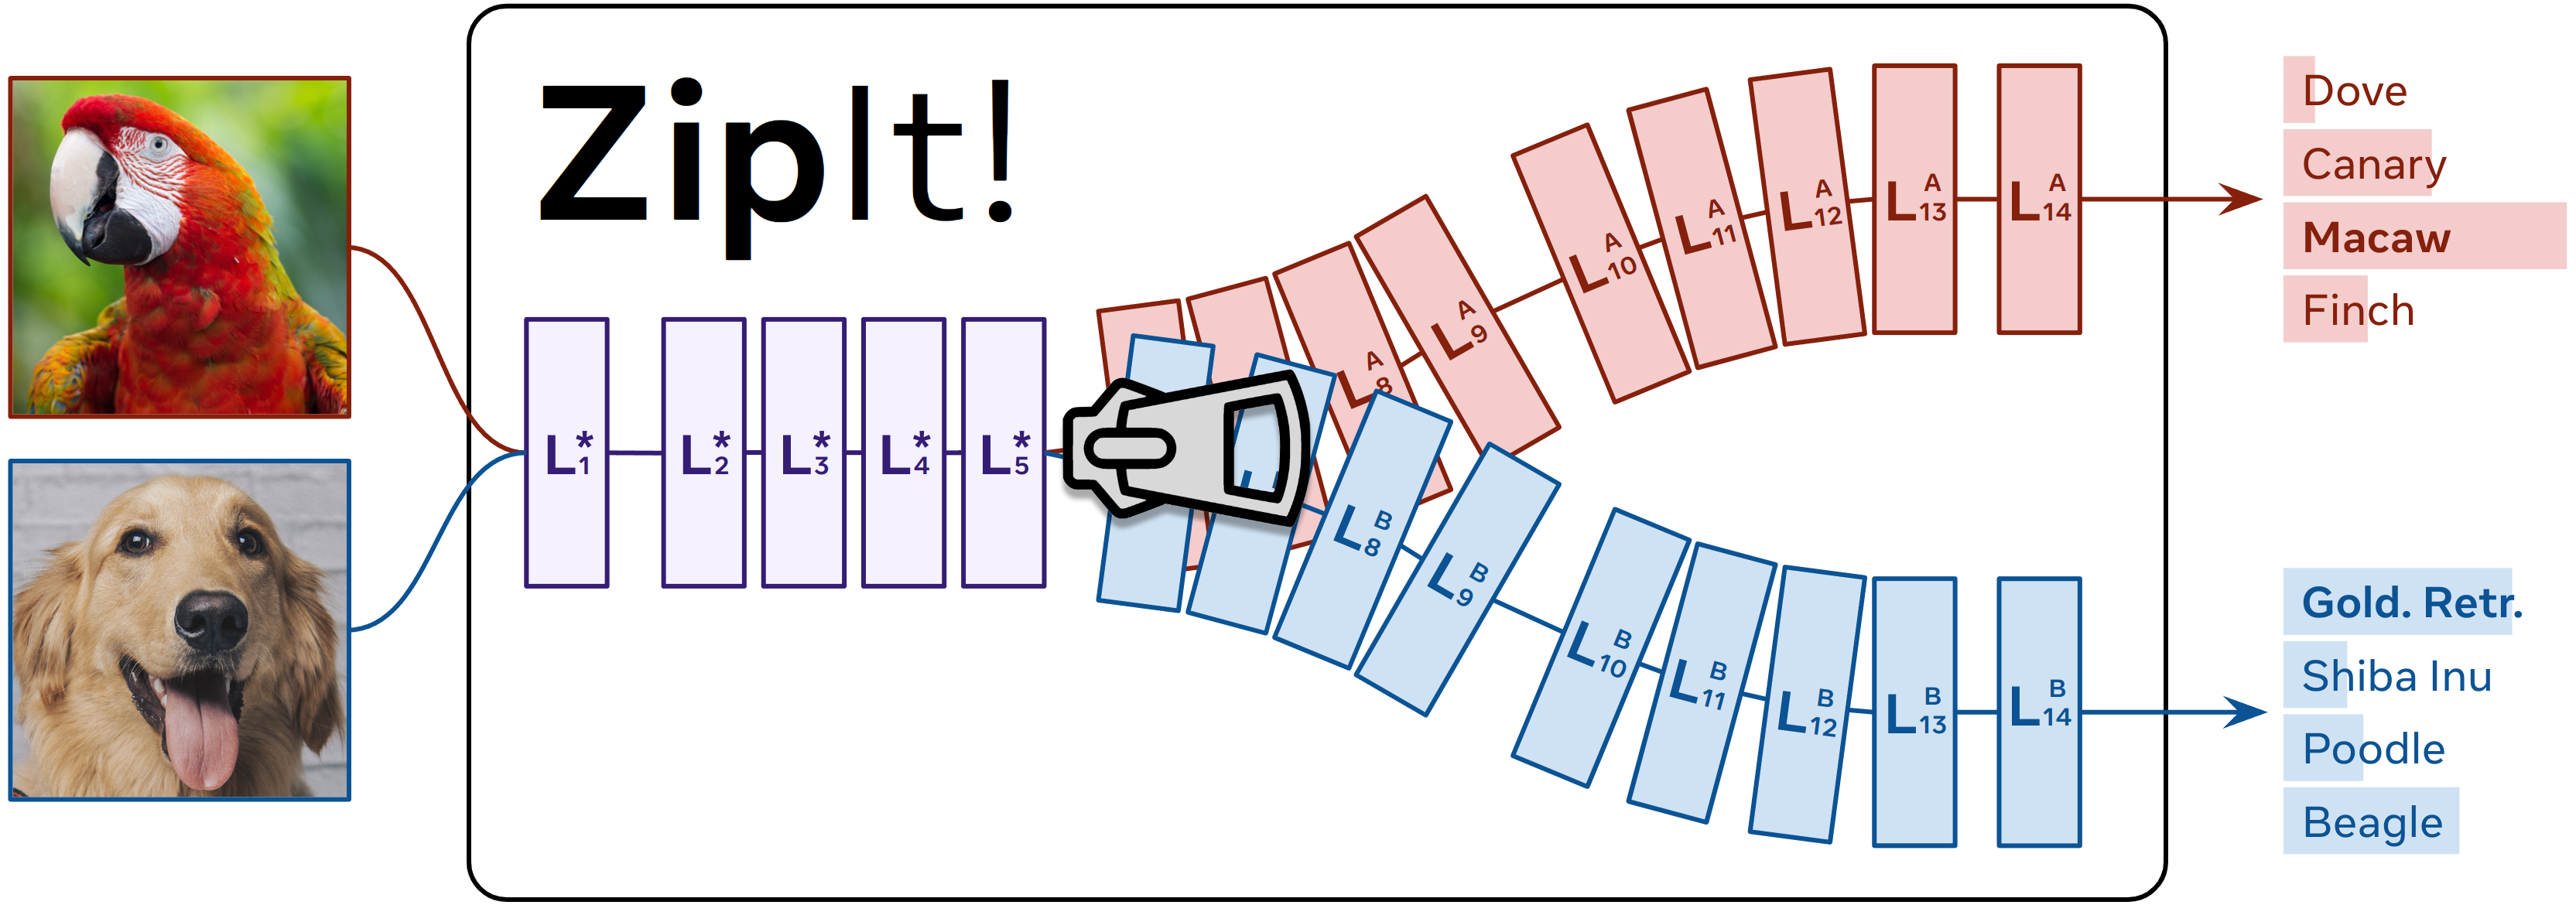
\includegraphics[width=\linewidth]{figures/imgs/concept.png}
%     \caption{{\bf \name{}} merges models trained on completely separate tasks \textit{without any additional training} by identifying their shared features.
%     Depending on the architecture and task, \name{} can nearly match their ensemble performance.
%     }
%     \label{fig:concept}
% }\end{minipage}
% \hspace{1em}
% \begin{minipage}{0.48\linewidth}{
%     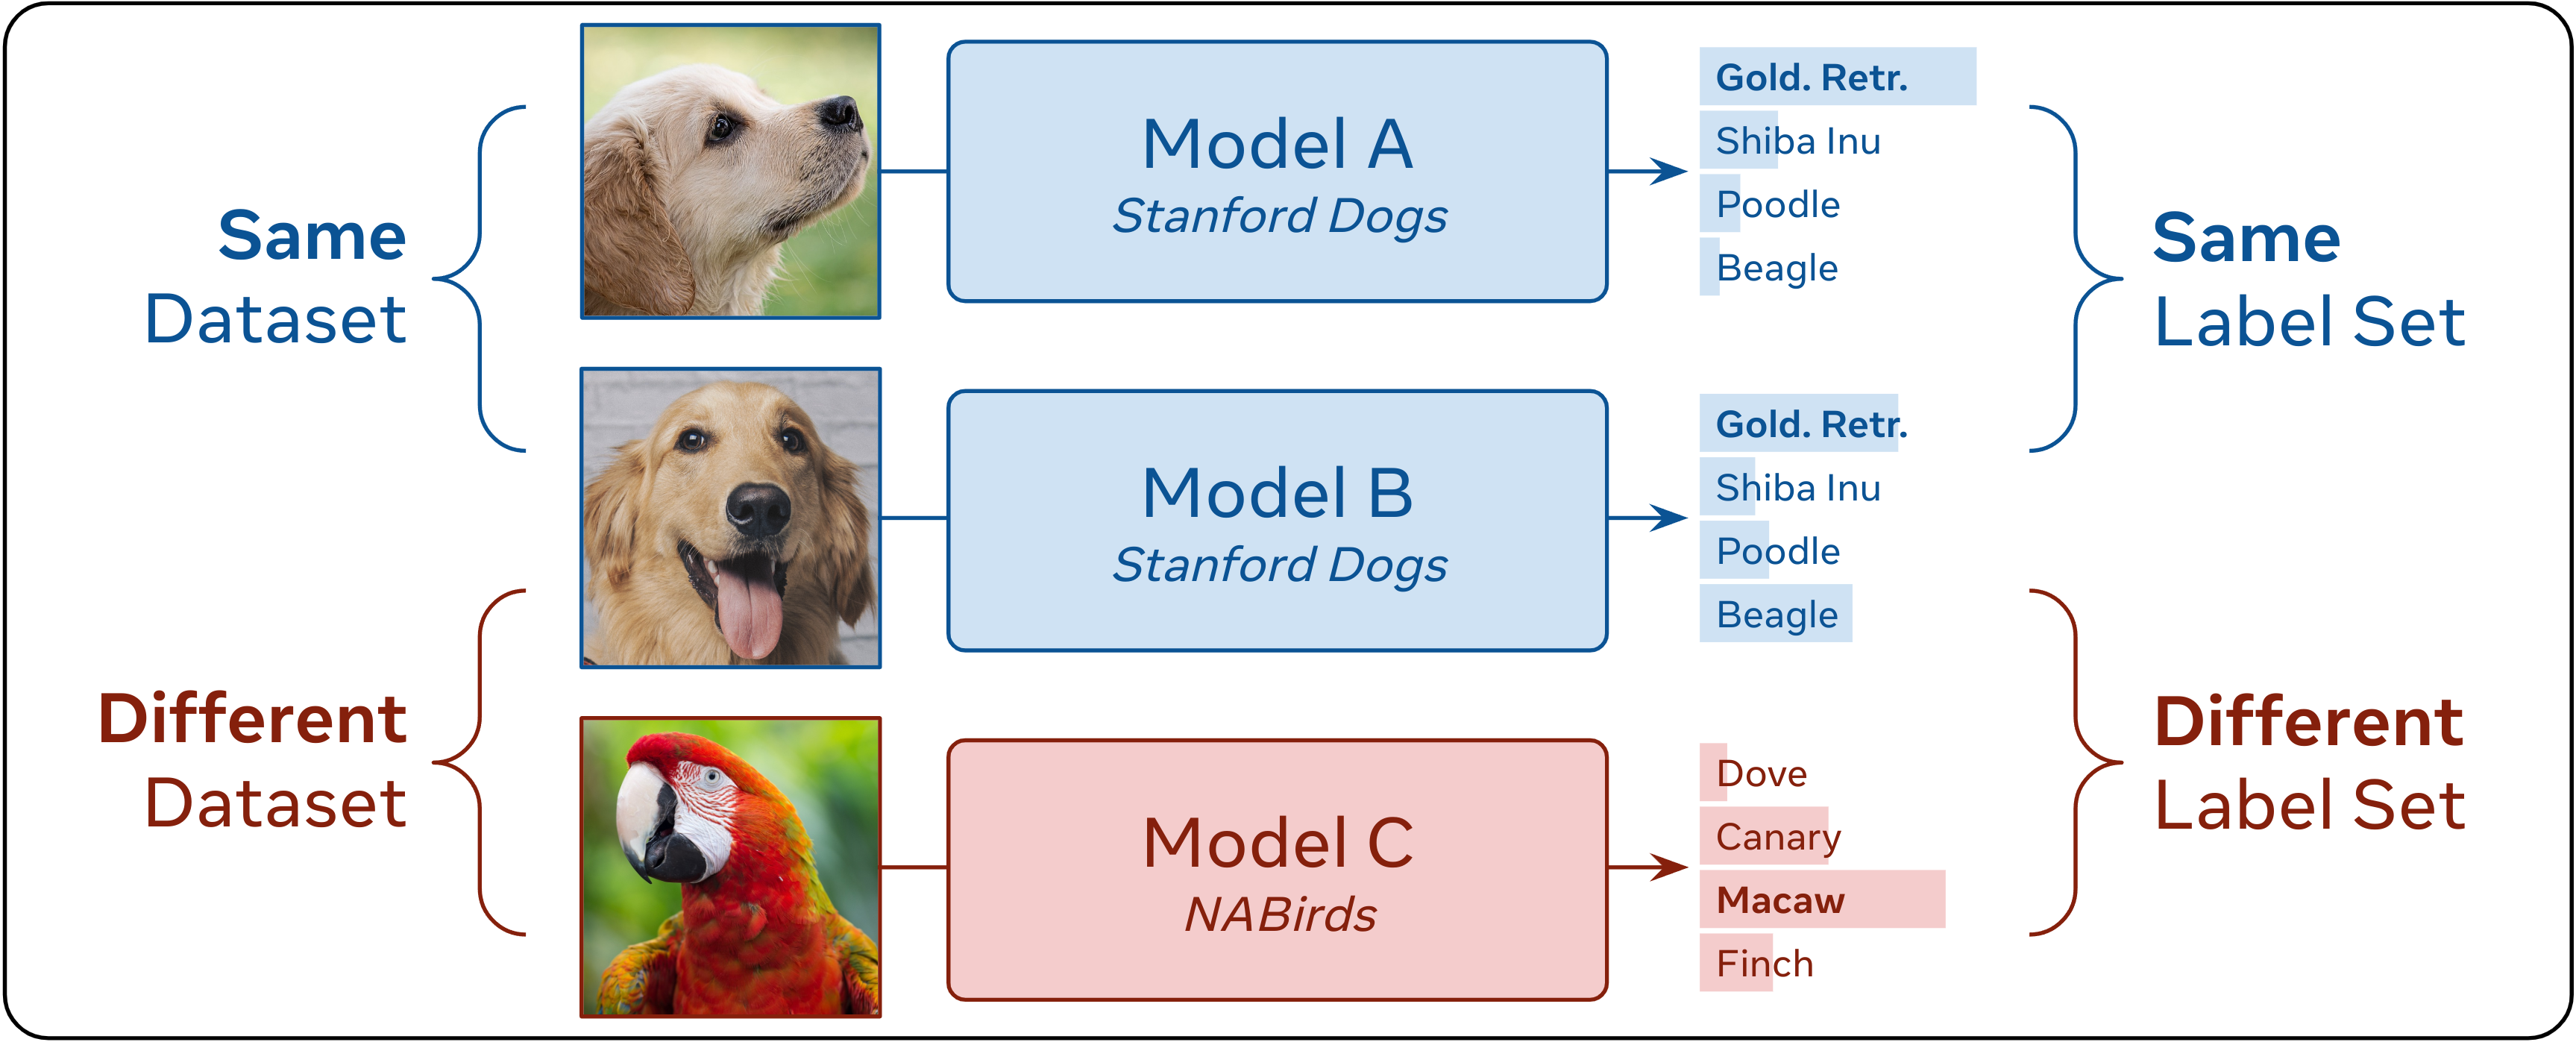
\includegraphics[width=\linewidth]{figures/imgs/vs_prior_work.png}
%     \caption{{\bf Our Setting.} Prior work \cite{wortsman2022model,ainsworth2022git,jordan2022repair}
%     focuses on merging models from the \modelb{\textbf{same} dataset} with the \modelb{\textbf{same} label sets}: e.g., merging two models both trained to classify dog breeds. In this work, we remove that restriction and ``zip'' models that can come from \modela{\textbf{different} datasets} and have \modela{\textbf{different} label sets}: e.g., merging a model that classifies dog breeds with one that classifies bird species.
%     }
%     \label{fig:capabilities}
%     % \includegraphics[width=\linewidth]{figures/imgs/random_r_experiment.png}
    
%     % \captionof{figure}{\textbf{Token Merging Schedule.} Our default constant merging schedule is close to optimal when compared to 15k randomly sampled merging schedules on an AugReg ViT-B/16. }
%     % \label{fig:r_ablation}
% }\end{minipage}
% \end{figure}


% #########################################################

\vspace{-0.5em}
\subsection{CIFAR-10 and CIFAR-100}
We train 5 pairs of ResNet-20 \cite{he2015deep} from scratch with different initializations on disjoint halves of the CIFAR-10 and CIFAR-100 classes \cite{krizhevsky2009cifar}. While \name{}\ supports ``partial zipping'' to merge models with different outputs (in this case, disjoint label sets), prior methods without retraining do not. To make a fair comparison, we train these CIFAR models with a CLIP-style loss \cite{radford2021learning} using CLIP text encodings of the class names as targets. 
This way, both models output into the same CLIP-space regardless of the category.
% That way, both models output into the same space, despite predicting different sets of categories. 
Note, this means the models are capable of some amount of zero-shot classification on the tasks they were not trained on.
% , and can get better than random accuracy on tasks they were not trained on.

% Thus, they get better than random accuracy on tasks they were not trained on.
% We also experiment with VGG models in this setting, and achieve similar results to our ResNet experiments (See Appendix~\ref{ap:vgg}).

\paragraph{CIFAR-10 (5+5).}
In Tab.~\ref{tab:cifar5+5}, we merge models trained on disjoint 5 class subsets of CIFAR-10 using ResNet-20 with a $4\times$ width multiplier (denoted as ResNet-20$\times$4). In joint classification (i.e., 10-way), Git Re-Basin is unable to perform better than using either of the original models alone, while our Permute baseline performs slightly better.
In stark contrast, our \name{}\ performs a staggering \textit{32.9\%} better than Git Re-Basin and \textit{20.7\%} better than our baseline.
If allow the last stage of the network to remain unzipped (i.e., zip up to 13 layers), our method obtains 83.8\%, which is only 3.6\% behind an ensemble of \modela{model A} and \modelb{model B} (which is practically the upper bound for this setting).
We also achieve similar results when merging VGG11 models in this setting (Appendix~\ref{ap:vgg}).

\vspace{-0.2em}
\paragraph{CIFAR-100 (50+50).}
We find similar results on disjoint 50 class splits of CIFAR-100 in Tab.~\ref{tab:cifar50+50}, this time using an $8\times$ width multiplier instead. Like with CIFAR-10, Git Re-Basin fails to outperform even the unmerged models themselves in joint classification (i.e., 100-way), and this time Permute is only 1.2\% ahead. \name{}\ again \textit{significantly} outperforms prior work with +14\% accuracy over Git Re-Basin for all layers zipped, and a substantial +29.2\% if zipping 13/20 layers. At this accuracy, \name{}$_{13/20}$ is again only 3.3\% behind the ensemble for joint accuracy and 2.6\% behind for average per task accuracy, landing itself in an entirely different performance tier compared to prior work.




% %##################################################################################################
\begin{wrapfigure}{r}{0.5\textwidth}
\vspace{-20pt}
\resizebox{0.48\textwidth}{!}{
% \begin{adjustbox}{max width=0.5\textwidth}

    \tablestyle{5pt}{1.1}
    \begin{tabular}{y{53}x{40}|x{30}x{30}x{30}x{30}}
        & & \multicolumn{4}{c}{Accuracies (\%)}\\
        Method & FLOPs (G) & Joint & \modela{Task A} & \modelb{Task B} & Avg \\
        \shline
        \modela{Model A} & {4.11} & {37.2\conf{2.0}} & {74.3\conf{4.0}} & {0.5\conf{0.1}} & {37.4\conf{2.0}} \\
        \modelb{Model B} & {4.11} & {35.3\conf{1.6}} & {0.5\conf{0.1}} & {70.5\conf{3.2}} & {35.5\conf{1.6}} \\
        \hline
        W. Avg \tiny{(Eq.~\ref{eq:wavg})} &4.11& {0.3\conf{0.1}} & {0.6\conf{0.1}} & {0.7\conf{0.1}} & {0.6\conf{0.1}} \\
        Git Re-Basin$^{\ddag}$ &4.11 & {3.1\conf{1.2}} & {5.3\conf{2.6}} & {5.7\conf{2.4}} & {5.5\conf{1.7}}  \\
        % Git Re-Basin \cite{ainsworth2022git}  &4.11 & {3.1\conf{1.2}} & {5.3\conf{2.6}} & {5.7\conf{2.4}} & {5.5\conf{1.7}}  \\
        Permute \tiny{(Eq.~\ref{eq:rebasin})} &4.11 & \textbf{8.6\conf{5.8}} & \textbf{10.1\conf{4.4}} & \textbf{15.3\conf{11.1}} & \textbf{12.7\conf{7.7}} \\
        \default{{\bf \name{}}$_\text{50/50}$} &4.11 & \textbf{8.6\conf{4.7}} & \textbf{12.4\conf{5.9}} & \textbf{14.7\conf{7.8}} & \textbf{13.5\conf{6.6}} \\
        \hline
        \gc{Ensemble} & \gc{8.22} & \gc{63.3\conf{4.9}} & \gc{74.3\conf{4.0}} & \gc{70.5\conf{3.2}} & \gc{72.4\conf{2.5}} \\
        % \default{{\bf \name{}}$_\text{37/50}$} & 4.92 & {33.1\conf{5.9}} & {41.8\conf{5.3}} & {42.3\conf{8.2}} & {42.0\conf{6.2}} \\
        \default{{\bf \name{}}$_\text{22/50}$} & 6.39 & {55.8\conf{4.1}} & {65.9\conf{2.5}} & {64.1\conf{3.0}} & {65.0\conf{2.3}} \\
        \default{{\bf \name{}}$_\text{10/50}$} & 7.43 & \textbf{60.9\conf{4.1}} & \textbf{70.7\conf{3.0}} & \textbf{69.0\conf{2.9}} & \textbf{69.9\conf{1.9}} \\
    \end{tabular}
% \end{adjustbox}
}

\captionof{table}{\textbf{ImageNet-1k (200+200) Results.} Merging ResNet-50 models trained from scratch on disjoint 200 category subsets (Task \modela{A} and \modelb{B}) of ImageNet-1k. Prior work performs poorly, but \name{}\ makes this task feasible. {$^\ddag$\scriptsize \citet{ainsworth2022git}.}
}
\label{tab:imagenet200x5}
\vspace{-14pt}
\end{wrapfigure}
% %##################################################################################################


% %##################################################################################################
% \begin{wrapfigure}{r}{0.5\textwidth}
% % \vspace{-150pt}
% \resizebox{0.48\textwidth}{!}{
% % \begin{adjustbox}{max width=0.5\textwidth}

%     \tablestyle{5pt}{1.1}
%     \begin{tabular}{y{52}x{20}x{28}|x{24}x{24}x{24}}
    
%         & FLOPs& Joint & \multicolumn{3}{c}{Per-Task (\%)}\\
%         Method & (G) & Acc (\%) & \modela{Task A} & \modelb{Task B} & Avg\\
%         \shline
%         \modela{Model A} & {4.11} & {37.2\conf{2.0}} & {74.3\conf{4.0}} & {0.5\conf{0.1}} & {37.4\conf{2.0}} \\
%         \modelb{Model B} & {4.11} & {35.3\conf{1.6}} & {0.5\conf{0.1}} & {70.5\conf{3.2}} & {35.5\conf{1.6}} \\
%         \hline
%         W. Avg \tiny{(Eq.~\ref{eq:wavg})} &4.11& {0.3\conf{0.1}} & {0.6\conf{0.1}} & {0.7\conf{0.1}} & {0.6\conf{0.1}} \\
%         Git Re-Basin$^{\ddag}$ &4.11 & {3.1\conf{1.2}} & {5.3\conf{2.6}} & {5.7\conf{2.4}} & {5.5\conf{1.7}}  \\
%         % Git Re-Basin \cite{ainsworth2022git}  &4.11 & {3.1\conf{1.2}} & {5.3\conf{2.6}} & {5.7\conf{2.4}} & {5.5\conf{1.7}}  \\
%         Permute \tiny{(Eq.~\ref{eq:rebasin})} &4.11 & \textbf{8.6\conf{5.8}} & \textbf{10.1\conf{4.4}} & \textbf{15.3\conf{11.1}} & \textbf{12.7\conf{7.7}} \\
%         \default{{\bf \name{}}$_\text{50/50}$} &4.11 & \textbf{8.6\conf{4.7}} & \textbf{12.4\conf{5.9}} & \textbf{14.7\conf{7.8}} & \textbf{13.5\conf{6.6}} \\
%         \hline
%         \gc{Ensemble} & \gc{8.22} & \gc{63.3\conf{4.9}} & \gc{74.3\conf{4.0}} & \gc{70.5\conf{3.2}} & \gc{72.4\conf{2.5}} \\
%         % \default{{\bf \name{}}$_\text{37/50}$} & 4.92 & {33.1\conf{5.9}} & {41.8\conf{5.3}} & {42.3\conf{8.2}} & {42.0\conf{6.2}} \\
%         \default{{\bf \name{}}$_\text{22/50}$} & 6.39 & {55.8\conf{4.1}} & {65.9\conf{2.5}} & {64.1\conf{3.0}} & {65.0\conf{2.3}} \\
%         \default{{\bf \name{}}$_\text{10/50}$} & 7.43 & \textbf{60.9\conf{4.1}} & \textbf{70.7\conf{3.0}} & \textbf{69.0\conf{2.9}} & \textbf{69.9\conf{1.9}} \\
%     \end{tabular}
% % \end{adjustbox}
% }

% \caption{\textbf{ImageNet-1k (200+200) Results.} Merging ResNet-50 models trained from scratch on disjoint 200 category subsets (Task \modela{A} and \modelb{B}) of ImageNet-1k. Prior work performs poorly, but \name{}\ makes this task feasible. $\ddag$ refers to \cite{ainsworth2022git}
% }
% \label{tab:imagenet200x5}
% \end{wrapfigure}
% %##################################################################################################
\vspace{-0.5em}
\subsection{ImageNet-1k (200+200)}
To test our method on the \textit{much harder} setting of large-scale data, we train 5 differently initialized ResNet-50 models with cross entropy loss on disjoint 200 class subsets of ImageNet-1k \cite{deng2009imagenet}.
To compare to prior work that doesn't support partial zipping, we initialize the models with capacity for all 1k classes, but only train each on their subset.

In Tab.~\ref{tab:imagenet200x5} we show results on exhaustively merging pairs from the 5 models. To compute joint (i.e., 400-way) accuracy, we softmax over each task's classes individually (like in \citet{ahn2021ss}), and take the argmax over the combined 400 class vector. On this extremely difficult task, Git Re-Basin only obtains 3.1\% for joint accuracy (with random accuracy being 0.25\%).
Both the Permute baseline and \name{}\ with all layers zipped perform better, but with each at 8.6\%, are still clearly lacking.
Note that we find the same-model merging budget $\beta$ to not matter for this set of models (see Fig.~\ref{fig:variations}), which suggests that there's not a lot of redundant information \textit{within} each model 
% for
in
this setting. Thus, \name{}\ chooses to merge mostly \textit{across} models instead, performing similarly to the permute baseline. We find this same trend in CIFAR with smaller models (see Fig.~\ref{fig:variations}), 
% so this 
and
may be an artifact of model capacity. 
% To that end, 
The story changes when we increase the capacity of the merged model by partial zipping: \name{}$_{10/50}$ 
% is able to reach 
reaches
close to upper bound ensemble accuracy \textit{on this extremely difficult task}, while saving on FLOPs.

\vspace{-0.5em}
\subsection{Multi-Dataset Merging}
We now take our model merging framework one step further by merging differently initialized models trained on \textit{completely separate datasets and tasks}. We present two settings: merging multiple classification datasets and merging semantic segmentation with image classification.

% in one we merge image classification models, and in the other we merge image generation models.
% We first present a setting where we merge models trained on different image classification datasets, and second a setting where we merge several image generation models.

% % Concatenated Table
% %##################################################################################################
% \begin{table*}[t]
% \centering
% \subfloat[
%     \textbf{Merging Model Pairs.} ResNet-50.
%     \label{tab:two_way}
% ]{
% \centering
% \begin{minipage}{0.47\linewidth}{
% \begin{center}
% \resizebox{\textwidth}{!}{
%     \tablestyle{5pt}{1.1}
%     {\renewcommand\conf[1]{}
%     \tablestyle{5pt}{1.1}
%     \begin{tabular}{y{50}x{40}|x{20}x{20}x{20}x{20}x{20}}
%         & & \multicolumn{5}{c}{Paired-Merge Per-Task Accuracies (\%)} \\
%         Method & FLOPs (G) & SD & OP & CUB & NAB & Avg\\
%         \shline
%         W. Avg \tiny{(Eq.~\ref{eq:wavg})} & {4.11} & {15.1\conf{18.8}} & {23.8\conf{43.3}} & {11.8\conf{19.2}} & {2.1\conf{3.2}} & {13.2\conf{9.0}}  \\
%         Permute \tiny{(Eq.~\ref{eq:rebasin})} & 4.11 & \textbf{51.3\conf{10.6}} & 64.7\conf{15.3} & 36.7\conf{17.8} & \textbf{15.5\conf{64.7}} & 42.1\conf{21.1} \\
%         \default{{\bf \name{}}$_\text{49/50}$} & 4.11 & \textbf{51.2\conf{9.4}} & \textbf{67.7\conf{17.6}} & \textbf{40.6\conf{19.1}} & \textbf{15.6\conf{12.2}} & \textbf{43.8\conf{21.8}} \\
%         \hline
%         \gc{Ensemble} & \gc{8.22} & \gc{72.7} & \gc{83.2} & \gc{71.0} & \gc{77.2} & \gc{76.0\conf{4.7}} \\
%         \default{{\bf \name{}}$_\text{37/50}$} & 4.92 & {56.8\conf{1.9}} & {73.8\conf{13.1}} & {54.6\conf{3.5}} & {37.9\conf{22.3}} & {55.8\conf{14.7}} \\
%         \default{{\bf \name{}}$_\text{22/50}$} & 6.39 & \textbf{65.3\conf{0.6}} & \textbf{79.7\conf{4.8}} & \textbf{64.8\conf{2.2}} & \textbf{61.2\conf{8.9}} & \textbf{67.7\conf{8.2}} \\
%     \end{tabular}
%     }
% }
% \end{center}
% }\end{minipage}
% }
% \hspace{1em}
% \centering
% \subfloat[
%     \textbf{Merging All Models.} ResNet-50.
%     \label{tab:cifar50+50}
% ]{
% \centering
% \begin{minipage}{0.47\linewidth}{
% \begin{center}
% \resizebox{\textwidth}{!}{
%     \tablestyle{5pt}{1.1}
%     {\renewcommand\conf[1]{}
%     \tablestyle{5pt}{1.1}
%     \begin{tabular}{y{50}x{40}|x{20}x{20}x{20}x{20}x{20}}
%         & & \multicolumn{5}{c}{All-Merged Per-Task Accuracies (\%)} \\
%         Method & FLOPs (G) & SD & OP & CUB & NAB & Avg\\
%         \shline
%         W. Avg \tiny{(Eq.~\ref{eq:wavg})} & {4.12} & {0.7} & {3.4} & {0.4} & {0.2} & {1.2\conf{1.5}}  \\
%         Permute \tiny{(Eq.~\ref{eq:rebasin})} & {4.12} & \textbf{34.2} & \textbf{55.4} & {13.4} & {5.7} & \textbf{27.2\conf{19.3}}  \\
%         \default{{\bf \name{}}$_\text{49/50}$} & {4.12} & {32.1} & \textbf{55.3} & \textbf{14.7} & \textbf{6.9} & \textbf{27.3\conf{20.1}}  \\
%         \hline
%         \gc{Ensemble} & \gc{16.44} & \gc{72.7} & \gc{83.2} & \gc{71.0} & \gc{77.2} & \gc{76.0\conf{4.7}} \\
%         \default{{\bf \name{}}$_\text{37/50}$} & {6.5} & {39.9} & {66.4} & {44.3} & {24.6} & {43.8\conf{17.2}}  \\
%         \default{{\bf \name{}}$_\text{22/50}$} & {11.0} & \textbf{58.2} & \textbf{78.5} & \textbf{58.6} & \textbf{55.1} & \textbf{62.6\conf{10.7}}  \\
%     \end{tabular}
%     }
% }
% \end{center}
% }\end{minipage}
% }
% \caption{\textbf{Multi-Dataset Results.} Merge differently initialized ResNet-50 models trained on \textit{disjoint datasets}: Stanford Dogs (SD), Oxford Pets (OP), CUB200 (CUB), and NABirds (NAB). 
% % We report average per-task accuracy over merging model pairs, and merging all four.
% }
% \label{tab:cross_dataset_results}
% % \vspace{-15pt}
% \end{table*}
%##################################################################################################
% Imnet200 P1 Table
% Stacked Table
%##################################################################################################

\begin{wrapfigure}{r}{0.48\linewidth}
\vspace{-20pt}
\centering
\resizebox{\linewidth}{!}{
    \tablestyle{5pt}{1.1}
    {\renewcommand\conf[1]{}
    \tablestyle{5pt}{1.1}
    \begin{tabular}{y{50}x{40}|x{20}x{20}x{20}x{20}x{20}}
        & & \multicolumn{5}{c}{Per-Task Accuracies (\%)} \\
        Method & FLOPs (G) & SD & OP & CUB & NAB & Avg\\
        \shline
        \multicolumn{7}{c}{Merging Pairs}\\
        \hline                                % FLOPS       Stanford Dogs               Oxford Pets                 CUB                         NA Birds                    Avg
        W. Avg \tiny{(Eq.~\ref{eq:wavg})}       & 4.11      & {12.9\conf{18.8}}         & {18.2\conf{43.3}}         & {13.9\conf{19.2}}         & {0.2\conf{3.2}}           & {11.3\conf{0.0}}  \\
        Permute \tiny{(Eq.~\ref{eq:rebasin})}   & 4.11      & 46.2\conf{15.5}            & 47.6\conf{16.6}           & 35.6\conf{24.7}           & \textbf{13.5\conf{14.9}}  & 35.7\conf{0.} \\
        \default{{\bf \name{}}$_\text{49/50}$}  & 4.11      & \textbf{46.9\conf{7.2}}   & \textbf{50.7\conf{13.0}}  & \textbf{38.0\conf{21.5}} & 12.7\conf{14.6}           & \textbf{37.1\conf{0}} \\
        \hline
        \gc{Ensemble}                           & \gc{8.22} & \gc{72.7}                 & \gc{81.1}                 & \gc{71.0}                 & \gc{77.2}                 & \gc{75.5\conf{4.7}} \\
        % \default{{\bf \name{}}$_\text{37/50}$}  & 4.92      & {53.9\conf{3.8}}          & {59.6\conf{6.0}}          & {52.8\conf{9.3}}         & {21.1\conf{14.4}}         & {46.9\conf{0.}} \\
        \default{{\bf \name{}}$_\text{22/50}$}  & 6.39      & {62.6\conf{2.3}}          & {71.2\conf{2.1}}          & {62.8\conf{5.3}}          & {53.0\conf{8.4}}          & {62.4\conf{0.}} \\
        \default{{\bf \name{}}$_\text{10/50}$}  & 7.42      & \textbf{66.5\conf{1.5}}   & \textbf{75.8\conf{1.9}}   & \textbf{65.6\conf{3.7}}   & \textbf{66.8\conf{4.0}}   & \textbf{68.7\conf{0.}} \\
        \hline
        \multicolumn{7}{c}{Merging All 4}\\
        \hline
        W. Avg \tiny{(Eq.~\ref{eq:wavg})}       & {4.12}    & {0.8}                     & {3.0}                     & {0.6}                     & {0.3}                     & {1.2\conf{1.5}}  \\
        Permute \tiny{(Eq.~\ref{eq:rebasin})}   & {4.12}    & {15.7}                    & {26.1}                    & \textbf{14.0}             & \textbf{5.3}              & {15.3\conf{19.3}}  \\
        \default{{\bf \name{}}$_\text{49/50}$}  & {4.12}    & \textbf{21.1}             & \textbf{33.3}             & {8.6}                     & {3.9}                     & \textbf{16.8\conf{20.1}}  \\
        \hline
        \gc{Ensemble}                           & \gc{16.4}& \gc{72.7}                 & \gc{81.2}                 & \gc{71.0}                 & \gc{77.2}                 & \gc{75.5\conf{4.7}} \\
        % \default{{\bf \name{}}$_\text{37/50}$}  & {6.5}     & {29.2}                    & {38.6}                    & {24.7}                    & {10.5}                    & {25.8\conf{17.2}}  \\
        \default{{\bf \name{}}$_\text{22/50}$}  & {11.0}    & {50.2}                    & {55.9}                    & {44.0}                    & {32.0}                    & {45.5\conf{10.7}}  \\
        \default{{\bf \name{}}$_\text{10/50}$}  & {14.1}    & \textbf{63.5}             & \textbf{70.8}             & \textbf{63.7}             & \textbf{63.1}             & \textbf{65.3\conf{10.7}}  \\
    \end{tabular}
    }
}
\captionof{table}{\textbf{Multi-Dataset Results.} Merging 
% differently initialized 
ResNet-50 models trained on \textit{completely different datasets}: Stanford Dogs (SD), Oxford Pets (OP), CUB200 (CUB), and NABirds (NAB). We report average per-task accuracy over merging model pairs, and all four.
% all pairs (2-way merging) and per-task accuracy for each head (4-way merging).
% We compare to our strong baseline as \cite{ainsworth2022git} doesn't support models with different outputs.
}
\label{tab:cross_dataset_results}
% \end{table}
\vspace{-20pt}
\end{wrapfigure}
% ##################################################################################################

% Table Partially filled in with Innet200 P0
% % Stacked Table
% %##################################################################################################

% \begin{wrapfigure}{r}{0.48\linewidth}
% \vspace{-10pt}
% \centering
% \resizebox{\linewidth}{!}{
%     \tablestyle{5pt}{1.1}
%     {\renewcommand\conf[1]{}
%     \tablestyle{5pt}{1.1}
%     \begin{tabular}{y{50}x{40}|x{20}x{20}x{20}x{20}x{20}}
%         & & \multicolumn{5}{c}{Per-Task Accuracies (\%)} \\
%         Method & FLOPs (G) & SD & OP & CUB & NAB & Avg\\
%         \shline
%         \multicolumn{7}{c}{Merging Pairs}\\
%         \hline
%         W. Avg \tiny{(Eq.~\ref{eq:wavg})} & {4.11} & {12.9\conf{18.8}} & {18.2\conf{43.3}} & {13.9\conf{19.2}} & {0.2\conf{3.2}} & {11.3\conf{9.0}}  \\
%         Permute \tiny{(Eq.~\ref{eq:rebasin})} & 4.11 & 46.2\conf{15.5} & 47.6\conf{16.6} & 35.6\conf{24.7} & \textbf{13.5\conf{14.9}} & 35.7\conf{21.1} \\
%         \default{{\bf \name{}}$_\text{49/50}$} & 4.11 & \textbf{46.9\conf{7.2}} & \textbf{50.7\conf{13.0}} & \textbf{38.0\conf{21.5}} & 12.7\conf{14.6} & \textbf{37.1\conf{21.8}} \\
%         \hline
%         \gc{Ensemble} & \gc{8.22} & \gc{72.7} & \gc{81.1} & \gc{71.0} & \gc{77.2} & \gc{76.0\conf{4.7}} \\
%         \default{{\bf \name{}}$_\text{37/50}$} & 4.92 & {53.9\conf{1.9}} & {59.6\conf{13.1}} & {52.8\conf{3.5}} & {21.1\conf{22.3}} & {46.9\conf{14.7}} \\
%         \default{{\bf \name{}}$_\text{22/50}$} & 6.39 & \textbf{62.6\conf{0.6}} & \textbf{71.2\conf{4.8}} & \textbf{62.8\conf{2.2}} & \textbf{53.0\conf{8.9}} & \textbf{62.4\conf{8.2}} \\
%         \hline
%         \multicolumn{7}{c}{Merging All 4}\\
%         \hline
%         W. Avg \tiny{(Eq.~\ref{eq:wavg})} & {4.12} & {0.7} & {3.4} & {0.4} & {0.2} & {1.2\conf{1.5}}  \\
%         Permute \tiny{(Eq.~\ref{eq:rebasin})} & {4.12} & \textbf{15.7} & \textbf{26.1} & {14.0} & {5.3} & \textbf{15.3\conf{19.3}}  \\
%         \default{{\bf \name{}}$_\text{49/50}$} & {4.12} & {32.1} & \textbf{55.3} & \textbf{14.7} & \textbf{6.9} & \textbf{27.3\conf{20.1}}  \\
%         \hline
%         \gc{Ensemble} & \gc{16.44} & \gc{72.7} & \gc{83.2} & \gc{71.0} & \gc{77.2} & \gc{76.0\conf{4.7}} \\
%         \default{{\bf \name{}}$_\text{37/50}$} & {6.5} & {39.9} & {66.4} & {44.3} & {24.6} & {43.8\conf{17.2}}  \\
%         \default{{\bf \name{}}$_\text{22/50}$} & {11.0} & \textbf{58.2} & \textbf{78.5} & \textbf{58.6} & \textbf{55.1} & \textbf{62.6\conf{10.7}}  \\
%     \end{tabular}
%     }
% }
% \captionof{table}{\textbf{Multi-Dataset Results.} Merging 
% % differently initialized 
% ResNet-50 models trained on \textit{completely different datasets}: Stanford Dogs (SD), Oxford Pets (OP), CUB200 (CUB), and NABirds (NAB). We report average per-task accuracy over merging model pairs, and all four.
% % all pairs (2-way merging) and per-task accuracy for each head (4-way merging).
% % We compare to our strong baseline as \cite{ainsworth2022git} doesn't support models with different outputs.
% }
% \label{tab:cross_dataset_results}
% % \end{table}
% \vspace{-20pt}
% \end{wrapfigure}
% % ##################################################################################################





% \begin{wrapfigure}{r}{0.48\linewidth}
% \vspace{-260pt}
% % \begin{minipage}{0.48\linewidth}{
% %     \centering
% %     \resizebox{\textwidth}{!}{
% %         \tablestyle{5pt}{1.1}
% %         {\renewcommand\conf[1]{}
% %         \tablestyle{5pt}{1.1}
% %         \begin{tabular}{y{50}x{20}|x{20}x{20}x{20}x{20}x{20}}
% %             & FLOPs & \multicolumn{5}{c}{Per-Task (\%)} \\
% %             Method & (G) & SD & OP & CUB & NAB & Avg\\
% %             \shline
% %             \multicolumn{7}{c}{Merging Pairs}\\
% %             \hline
% %             W. Avg \tiny{(Eq.~\ref{eq:wavg})} & {4.11} & {15.1\conf{18.8}} & {23.8\conf{43.3}} & {11.8\conf{19.2}} & {2.1\conf{3.2}} & {13.2\conf{9.0}}  \\
% %             Permute \tiny{(Eq.~\ref{eq:rebasin})} & 4.11 & \textbf{51.3\conf{10.6}} & 64.7\conf{15.3} & 36.7\conf{17.8} & \textbf{15.5\conf{64.7}} & 42.1\conf{21.1} \\
% %             \default{{\bf \name{}}$_\text{49/50}$} & 4.11 & \textbf{51.2\conf{9.4}} & \textbf{67.7\conf{17.6}} & \textbf{40.6\conf{19.1}} & \textbf{15.6\conf{12.2}} & \textbf{43.8\conf{21.8}} \\
% %             \hline
% %             \gc{Ensemble} & \gc{8.22} & \gc{72.7} & \gc{83.2} & \gc{71.0} & \gc{77.2} & \gc{76.0\conf{4.7}} \\
% %             \default{{\bf \name{}}$_\text{37/50}$} & 4.92 & {56.8\conf{1.9}} & {73.8\conf{13.1}} & {54.6\conf{3.5}} & {37.9\conf{22.3}} & {55.8\conf{14.7}} \\
% %             \default{{\bf \name{}}$_\text{22/50}$} & 6.39 & \textbf{65.3\conf{0.6}} & \textbf{79.7\conf{4.8}} & \textbf{64.8\conf{2.2}} & \textbf{61.2\conf{8.9}} & \textbf{67.7\conf{8.2}} \\
% %             \hline
% %             \multicolumn{7}{c}{Merging All 4}\\
% %             \hline
% %             W. Avg \tiny{(Eq.~\ref{eq:wavg})} & {4.12} & {0.7} & {3.4} & {0.4} & {0.2} & {1.2\conf{1.5}}  \\
% %             Permute \tiny{(Eq.~\ref{eq:rebasin})} & {4.12} & \textbf{34.2} & \textbf{55.4} & {13.4} & {5.7} & \textbf{27.2\conf{19.3}}  \\
% %             \default{{\bf \name{}}$_\text{49/50}$} & {4.12} & {32.1} & \textbf{55.3} & \textbf{14.7} & \textbf{6.9} & \textbf{27.3\conf{20.1}}  \\
% %             \hline
% %             \gc{Ensemble} & \gc{16.44} & \gc{72.7} & \gc{83.2} & \gc{71.0} & \gc{77.2} & \gc{76.0\conf{4.7}} \\
% %             \default{{\bf \name{}}$_\text{37/50}$} & {6.5} & {39.9} & {66.4} & {44.3} & {24.6} & {43.8\conf{17.2}}  \\
% %             \default{{\bf \name{}}$_\text{22/50}$} & {11.0} & \textbf{58.2} & \textbf{78.5} & \textbf{58.6} & \textbf{55.1} & \textbf{62.6\conf{10.7}}  \\
% %         \end{tabular}
% %         }
% %     }
% %     \captionof{table}{\textbf{Multi-Dataset Results.} Merging pairs of differently initialized ResNet-50 models trained on \textit{completely different datasets}: Stanford Dogs (SD), Oxford Pets (OP), CUB200 (CUB), and NABirds (NAB). We report average per-task accuracy over all pairs (2-way merging) and per-task accuracy for each head (4-way merging).
% %     We compare to our strong baseline as \cite{ainsworth2022git} doesn't support models with different outputs.
% %     }
% %     \label{tab:cross_dataset_results}
% %     % \end{table}

% % }\end{minipage}
% % \hfill

% \begin{minipage}[c]{\linewidth}{

%     \begin{minipage}[c]{\linewidth}
%         \resizebox{\textwidth}{!}{
%         % \begin{adjustbox}{max width=0.5\textwidth}
        
%             \tablestyle{5pt}{1.1}
%             \begin{tabular}{y{53}x{40}|x{30}x{30}x{30}x{30}}
%                 & & \multicolumn{4}{c}{Accuracies (\%)}\\
%                 Method & FLOPs (G) & Joint & \modela{Task A} & \modelb{Task B} & Avg \\
%                 \shline
%                 \modela{Model A} & {4.11} & {37.2\conf{2.0}} & {74.3\conf{4.0}} & {0.5\conf{0.1}} & {37.4\conf{2.0}} \\
%                 \modelb{Model B} & {4.11} & {35.3\conf{1.6}} & {0.5\conf{0.1}} & {70.5\conf{3.2}} & {35.5\conf{1.6}} \\
%                 \hline
%                 W. Avg \tiny{(Eq.~\ref{eq:wavg})} &4.11& {0.3\conf{0.1}} & {0.6\conf{0.1}} & {0.7\conf{0.1}} & {0.6\conf{0.1}} \\
%                 Git Re-Basin$^{\ddag}$ &4.11 & {3.1\conf{1.2}} & {5.3\conf{2.6}} & {5.7\conf{2.4}} & {5.5\conf{1.7}}  \\
%                 % Git Re-Basin \cite{ainsworth2022git}  &4.11 & {3.1\conf{1.2}} & {5.3\conf{2.6}} & {5.7\conf{2.4}} & {5.5\conf{1.7}}  \\
%                 Permute \tiny{(Eq.~\ref{eq:rebasin})} &4.11 & \textbf{8.6\conf{5.8}} & \textbf{10.1\conf{4.4}} & \textbf{15.3\conf{11.1}} & \textbf{12.7\conf{7.7}} \\
%                 \default{{\bf \name{}}$_\text{50/50}$} &4.11 & \textbf{8.6\conf{4.7}} & \textbf{12.4\conf{5.9}} & \textbf{14.7\conf{7.8}} & \textbf{13.5\conf{6.6}} \\
%                 \hline
%                 \gc{Ensemble} & \gc{8.22} & \gc{63.3\conf{4.9}} & \gc{74.3\conf{4.0}} & \gc{70.5\conf{3.2}} & \gc{72.4\conf{2.5}} \\
%                 % \default{{\bf \name{}}$_\text{37/50}$} & 4.92 & {33.1\conf{5.9}} & {41.8\conf{5.3}} & {42.3\conf{8.2}} & {42.0\conf{6.2}} \\
%                 \default{{\bf \name{}}$_\text{22/50}$} & 6.39 & {55.8\conf{4.1}} & {65.9\conf{2.5}} & {64.1\conf{3.0}} & {65.0\conf{2.3}} \\
%                 \default{{\bf \name{}}$_\text{10/50}$} & 7.43 & \textbf{60.9\conf{4.1}} & \textbf{70.7\conf{3.0}} & \textbf{69.0\conf{2.9}} & \textbf{69.9\conf{1.9}} \\
%             \end{tabular}
%         % \end{adjustbox}
%         }
        
%         \caption{\textbf{ImageNet-1k (200+200) Results.} Merging ResNet-50 models trained from scratch on disjoint 200 category subsets (Task \modela{A} and \modelb{B}) of ImageNet-1k. Prior work performs poorly, but \name{}\ makes this task feasible. $\ddag$ refers to \cite{ainsworth2022git}
%         }
%         \label{tab:imagenet200x5}
%     \end{minipage}
%     \begin{minipage}[c]{\linewidth}
%         \centering
%         \resizebox{\textwidth}{!}{
%             \tablestyle{7pt}{1.05}
%             \begin{tabular}{y{55}x{43}x{22}x{30}}
%                 Algorithm & \modela{A}$\leftrightarrow$\modela{A}/\modelb{B}$\leftrightarrow$\modelb{B}? & Acc & Time\\
%                 \shline
%                 Identity {\scriptsize (Eq.~\ref{eq:wavg})}                  & \xmark{} & {43.0\conf{3.1}} & {1.8\unit{ms}} \\
%                 Permute {\scriptsize (Eq.~\ref{eq:rebasin})}                & \xmark{} & {58.4\conf{1.3}} & {28\unit{ms}} \\
%                 K-Means                                                     & \checkmark{} & {29.1\conf{5.5}} & {19\unit{sec}} \\
%                 \hline
%                 \multicolumn{4}{c}{Zip {\scriptsize (Eq.~\ref{eq:zip})}} \\
%                 Optimal Match                                               & \checkmark{} & {\bf 79.6\conf{1.7}} & {11\unit{min}} \\
%                 Greedy Match                                                & \checkmark{} & {\bf 79.0\conf{1.8}} & {1.1\unit{sec}} \\
%                 Greedy, $\alpha$=0.1 & \default{\checkmark{}} & \default{\textbf{79.1\conf{2.1}}}  &  \default{1.2\unit{sec}}  \\
%             \end{tabular}
%         }
%         \captionof{table}{{\bf Matching Algorithm} to use for \modelc{$M_i$}. 
%         Permuting \modelb{B}$\rightarrow$\modela{A} as in prior work (Eq.~\ref{eq:rebasin}) performs poorly, thus we allow merging features \textit{within} each model (Eq.~\ref{eq:zip}).
%         Our greedy approach is nearly as accurate as the optimal algorithm while being two orders of magnitude faster. 
%         ``Acc'' is CIFAR-10 (5+5) joint 10-way accuracy.
%         }
%         \label{tab:matching_alg}
%     \end{minipage}
%     \vspace{10pt}
%     \begin{minipage}[c]{\linewidth}
%         % \vspace{40pt}
%         \centering
%         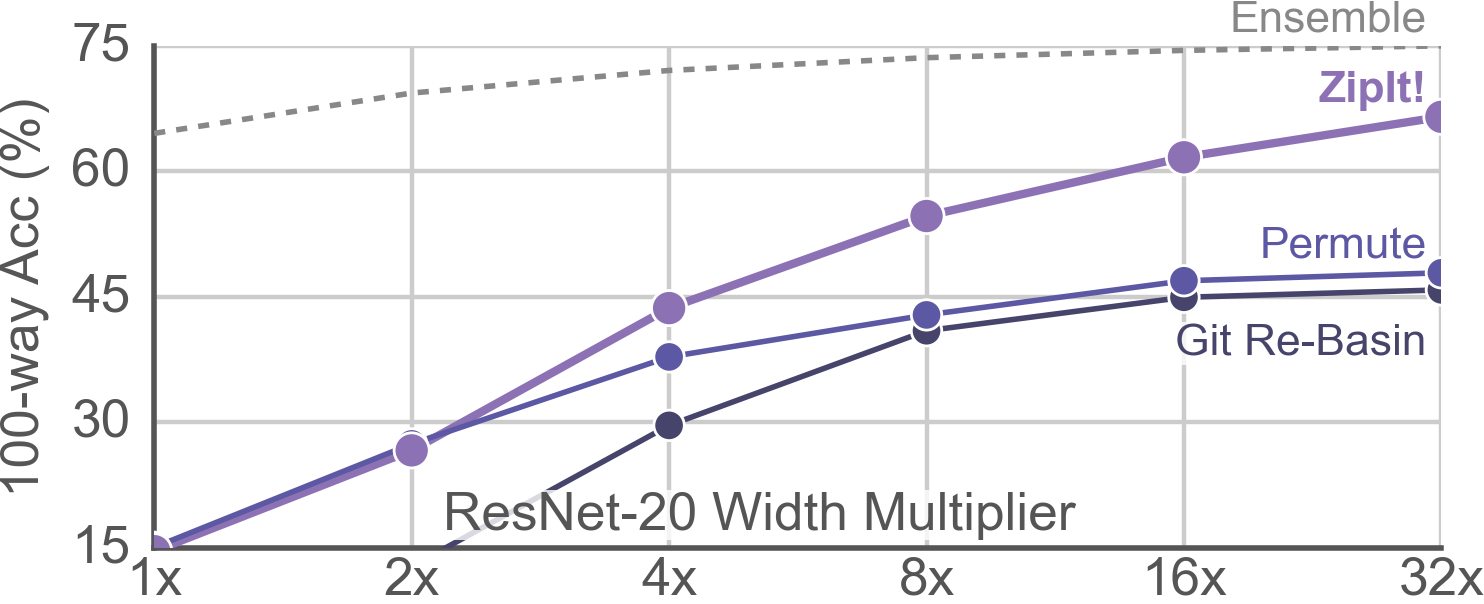
\includegraphics[width=0.95\linewidth]{figures/imgs/model_scale.png}
%         \caption{{\bf Model Scale.} As we increase the width of the ResNet-20 models used for the CIFAR-100 (50+50) setting, \name{}\ makes effective use of that extra capacity, quickly approaching ensemble accuracy. 
%         Git Re-Basin \cite{ainsworth2022git} and Permute only slightly benefit from the extra scale.
%         }
%         \label{fig:model_size}
%         % \vspace{-60pt}
%     \end{minipage}
% }\end{minipage}
% \end{wrapfigure}

\paragraph{Image Classification Datasets.}
% In this experiment, we take disjoint task model merging one step further by merging ResNet-50 models with different initializations trained on \textbf{four} \textit{completely separate datasets}, each with a different set of labels
Merging ResNet-50 models trained on: Stanford Dogs \cite{khosla2011stanforddogs}, Oxford Pets \cite{parkhi2012oxfordpets}, CUB200 \cite{welinder2010cub200}, and NABirds \cite{van2015buildingNaBird}. In Tab.~\ref{tab:cross_dataset_results},
we show the average per task accuracy from exhaustively merging each pair and the much more difficult setting of merging all four at once.
% we show the average per task accuracy for each dataset both if we exhaustively merge each pair and also the much more difficult setting of merging all four at once. 
We report the accuracy of our baselines by applying them up until the last layer, but we can't compare to prior work as they don't support this setting. As in all our previous experiment we merge \textit{without retraining}.

For pairs of models, \name{}\ slightly outperforms our permute baseline across all tasks and performs similarly when merging all 4 models at once.
% And for merging all 4 models at once, we perform similarly to permuting. 
However, if we add capacity to the merged model through partial zipping, we perform up to 33\% better on merging pairs and 50\% better on merging all four models than the permute baseline. Partial zipping is a significant factor to obtain strong performance, especially with more than 2 models.

\paragraph{Multiple Output Modalities.} In Appendix~\ref{appendix:semantic_segmentation}, we combine across modalities by merging the ResNet-50 backbone of a DeeplabV3 \cite{chen2017deeplabv3} segmentation model with an ImageNet-1k classification model. The resulting combined model can perform both semantic segmentation and image classification. Even with half of layers merged, \name{}\ retains good performance on both tasks.

\begin{figure}
    \centering
    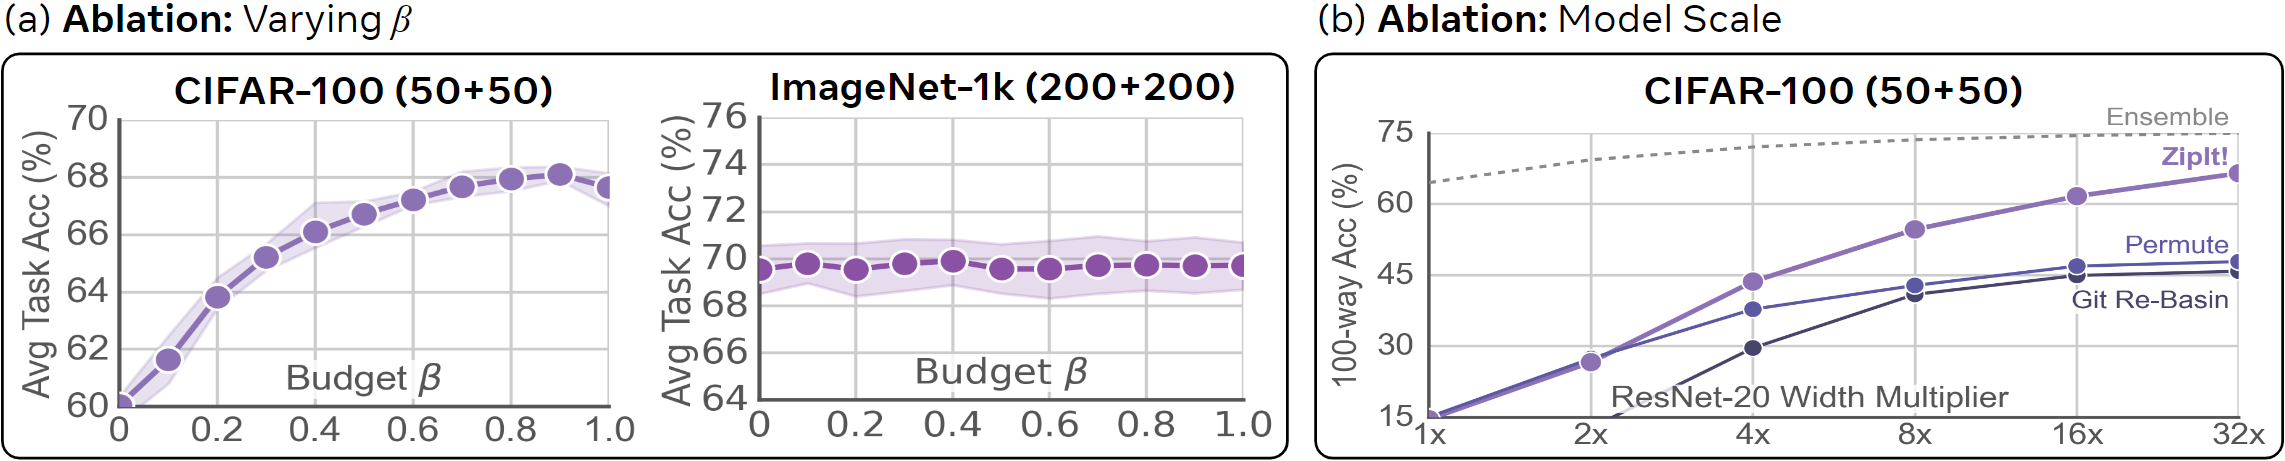
\includegraphics[width=\linewidth]{figures/imgs/varying_beta_and_scale.png}
    \caption{{\bf Varying $\beta$ and Model Scale.} 
    Left: 
    % we test the importance of same model matches by varying the budget $\beta$. A budget of 0 means no same-model matches are allowed, while 1 places no restrictions. 
    We find when the model has enough capacity for the task, a high budget (Sec.~\ref{sec:partial_zip}) improves performance. 
    Right: 
    \name{}\ makes effective use of extra model capacity to quickly reach the ensemble on CIFAR-100 (50+50) when we increase the width of ResNet-20 models. 
    In contrast, our baselines only slightly benefit from the extra scale.
    % Git Re-Basin \cite{ainsworth2022git} and Permute only slightly benefit from the extra scale.
% Git Re-Basin \cite{ainsworth2022git} and Permute only slightly benefit from the extra scale.
    }
    \label{fig:variations}
    % \vspace{-10pt}
\end{figure}

% \begin{figure}
%     \centering
%     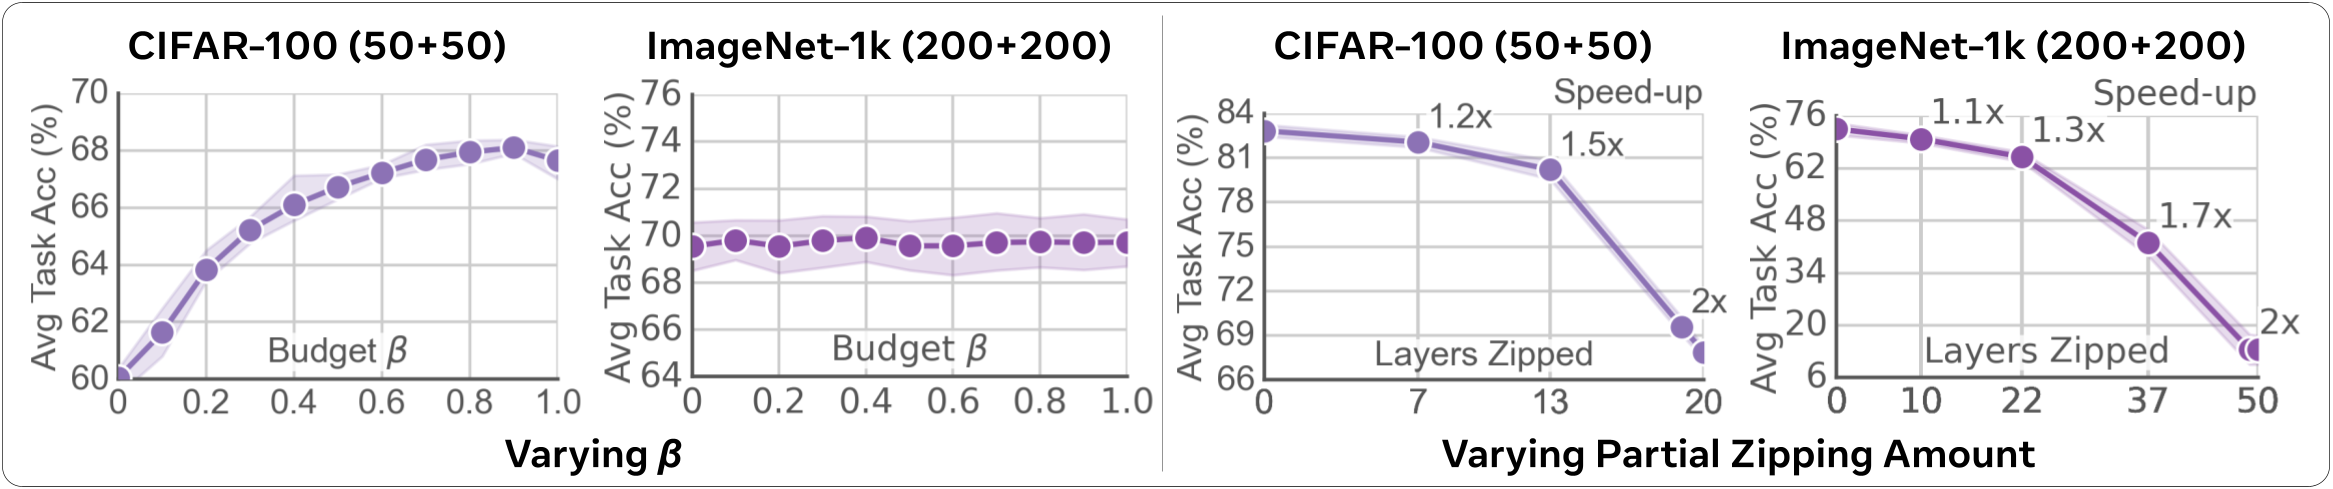
\includegraphics[width=\linewidth]{figures/imgs/zipit_varying_ablations.png}
%     \caption{{\bf Varying $\beta$ and Partial Zipping} (Sec.~\ref{sec:partial_zip}). Left: we test the importance of same model matches by varying the budget $\beta$. A budget of 0 means no same-model matches are allowed, while 1 places no restrictions. We find when the model has enough capacity for the task, a high budget improves performance. Right: by leaving some layers unzipped, we can recover a significant amount of performance while still merging most of the model. 
%     }
%     \label{fig:variations}
% \end{figure}


% \begin{figure}
%     \begin{minipage}[t]{0.48\linewidth}
%         \centering
%         \subfloat[
%             \textbf{CIFAR-100 50+50.}
%             \label{fig:budget_ablation_cifar100}
%         ]{
%             \centering
%             \begin{minipage}{0.48\linewidth}{
%                 \centering
%                 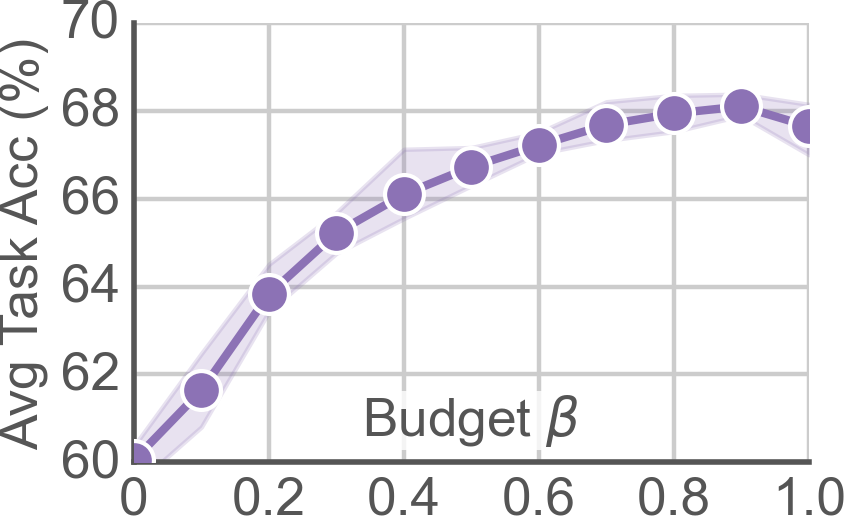
\includegraphics[width=\linewidth]{figures/imgs/cifar100_budget.png}
%             }\end{minipage}
%         }
%         \subfloat[
%             \textbf{ImageNet-1k 200+200.}
%             \label{fig:budget_ablation_imagenet}
%         ]{
%             \centering
%             \begin{minipage}{0.48\linewidth}{
%                 \centering
%                 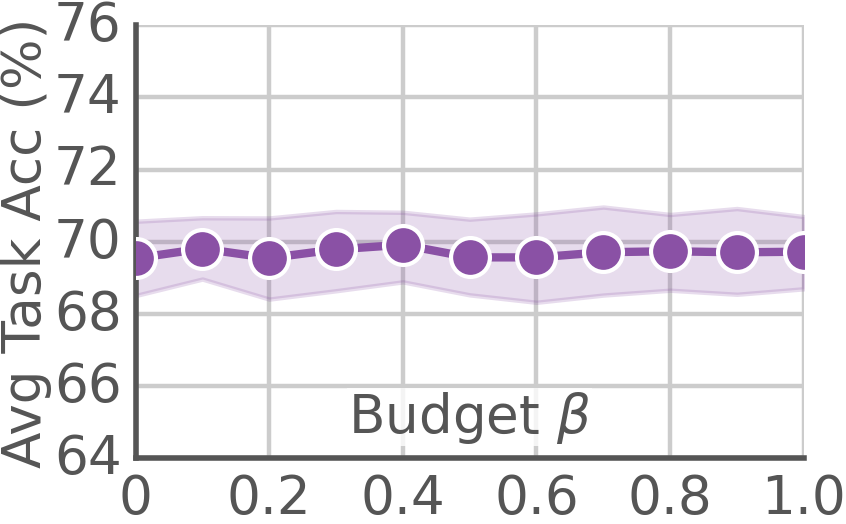
\includegraphics[width=\linewidth]{figures/imgs/imnet_budget.png}
%             }\end{minipage}
%         }
%         \caption{{\bf Varying $\beta$.} We test the importance of same model matches by varying the budget $\beta$ (Sec.~\ref{sec:partial_zip}). A budget of 0 means no same-model matches are allowed, while 1 places no restrictions. We find when the model has enough capacity for the task, a high budget improves performance. }
%         \label{fig:budget_ablation}
%         % \vspace{-80pt}
%     \end{minipage}
%     \hspace{1pt}
%     % \vspace{1em} % Add vertical space between the images
%     \begin{minipage}[t]{0.48\linewidth}
%         \centering
%         \subfloat[
%             \textbf{CIFAR-100 50+50.}
%             \label{fig:partial_zip_cifar100}
%         ]{
%             \centering
%             \begin{minipage}{0.49\linewidth}{
%                 \centering
%                 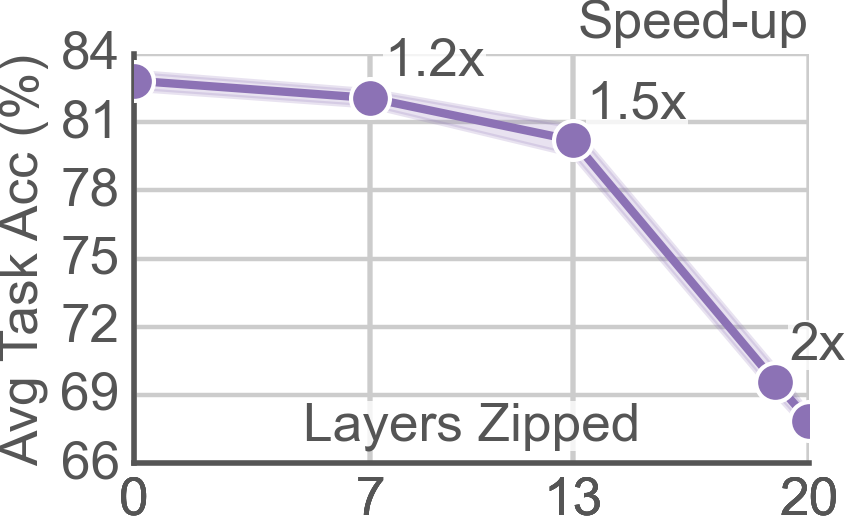
\includegraphics[width=\linewidth]{figures/imgs/partial_zip_CIFAR_50_50.png}
%             }\end{minipage}
%         }
%         \subfloat[
%             \textbf{ImageNet-1k 200+200.}
%             \label{fig:partial_zip_imagenet}
%         ]{
%             \centering
%             \begin{minipage}{0.49\linewidth}{
%                 \centering
%                 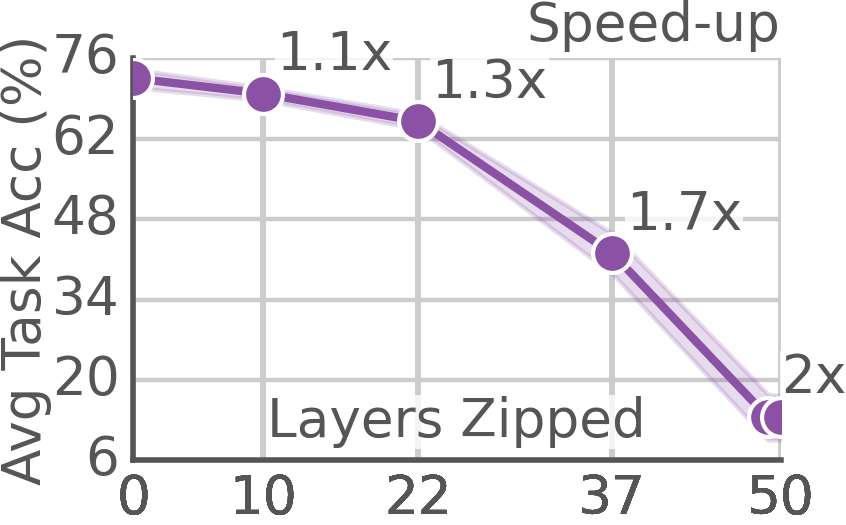
\includegraphics[width=\linewidth]{figures/imgs/partial_zip_imnet_200_200.png}
%             }\end{minipage}
%         }
%         \caption{
%         {\bf Varying Partial Zip.} 
%         By leaving some layers unzipped (Sec.~\ref{sec:partial_zip}), we can recover a significant amount of performance while still merging most of the model. 
%         }
%         \label{fig:varying_partial_zip}
%         % \vspace{10pt}
%     \end{minipage}
%     % \caption{Overall caption for the three images}
%     \vspace{-20pt}
% \end{figure}


%###################



% \begin{figure}[t]
% \centering

% \subfloat[
%     \textbf{CIFAR-100 50+50.}
%     \label{fig:budget_ablation_cifar100}
% ]{
% \centering
% \begin{minipage}{0.48\linewidth}{
% \begin{center}
%     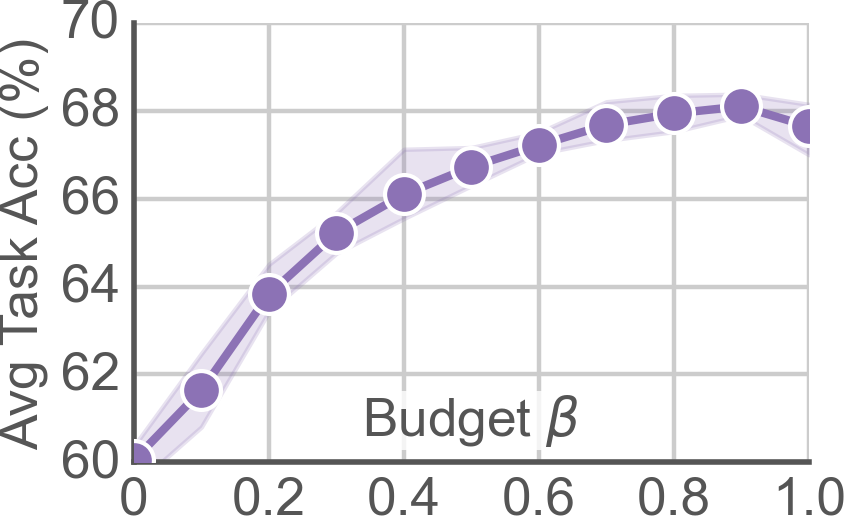
\includegraphics[width=\linewidth]{figures/imgs/cifar100_budget.png}
% \end{center}
% }\end{minipage}
% }
% \subfloat[
%     \textbf{ImageNet-1k 200+200.}
%     \label{fig:budget_ablation_imagenet}
% ]{
% \centering
% \begin{minipage}{0.48\linewidth}{
% \begin{center}
%     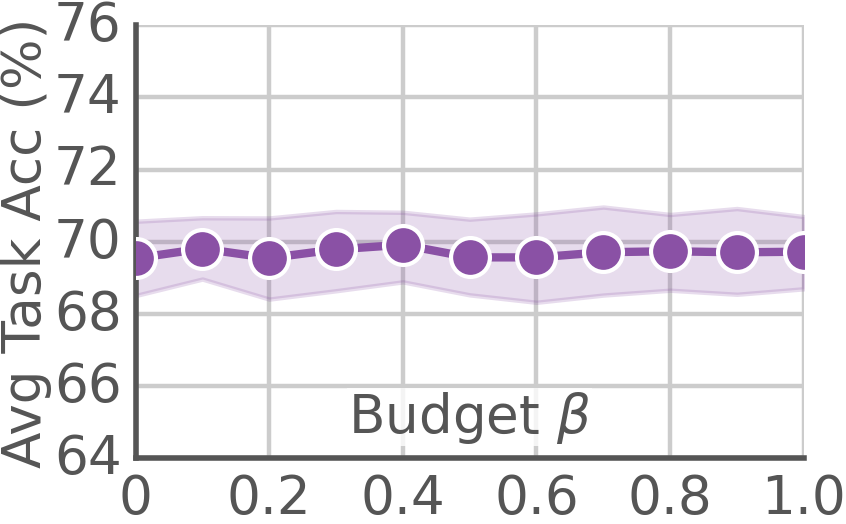
\includegraphics[width=\linewidth]{figures/imgs/imnet_budget.png}
% \end{center}
% }\end{minipage}
% }

% \caption{{\bf Varying $\beta$.} We test the importance of same model matches by varying the budget $\beta$ (Sec.~\ref{sec:partial_zip}). A budget of 0 means no same-model matches are allowed, while 1 places no restrictions. We find when the model has enough capacity for the task, a high budget improves performance. }
% \label{fig:budget_ablation}
% \end{figure}




% \begin{figure}[t]
% \centering

% \subfloat[
%     \textbf{CIFAR-100 50+50.}
%     \label{fig:partial_zip_cifar100}
% ]{
% \centering
% \begin{minipage}{0.49\linewidth}{
% \begin{center}
%     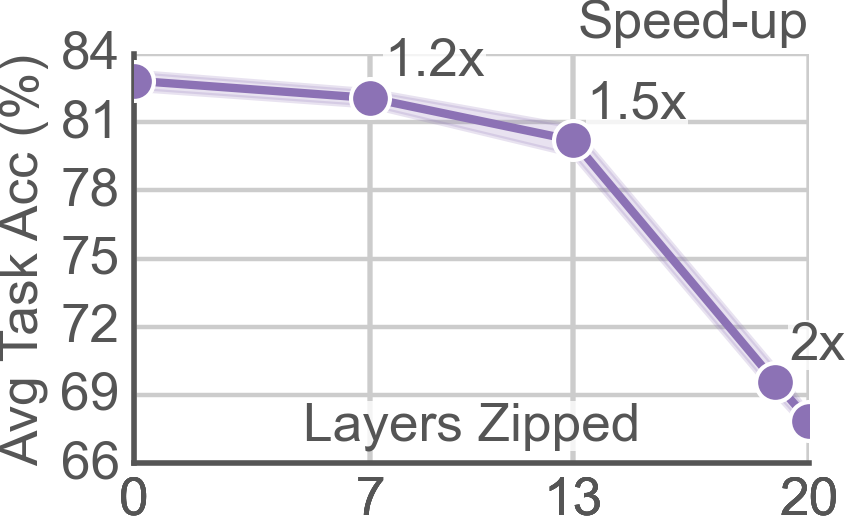
\includegraphics[width=\linewidth]{figures/imgs/partial_zip_CIFAR_50_50.png}
% \end{center}
% }\end{minipage}
% }
% \subfloat[
%     \textbf{ImageNet-1k 200+200.}
%     \label{fig:partial_zip_imagenet}
% ]{
% \centering
% \begin{minipage}{0.49\linewidth}{
% \begin{center}
%     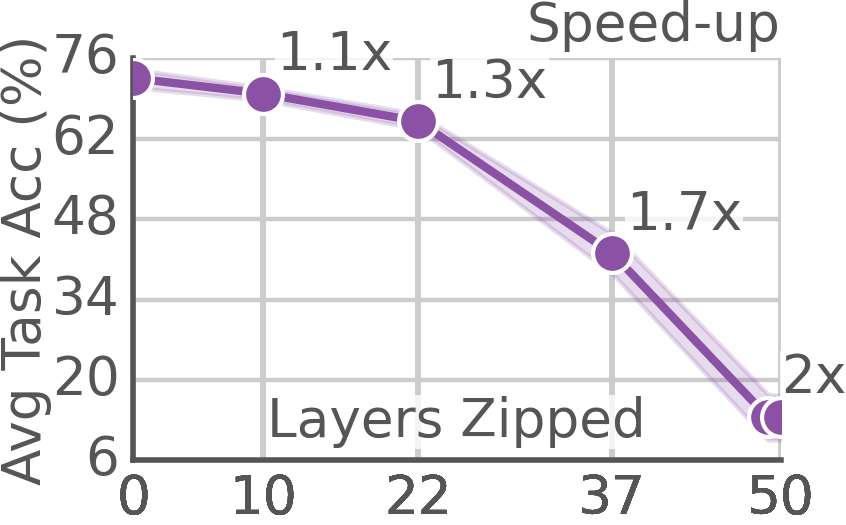
\includegraphics[width=\linewidth]{figures/imgs/partial_zip_imnet_200_200.png}
% \end{center}
% }\end{minipage}
% }

% \caption{
% {\bf Varying Partial Zip.} 
% By leaving some layers unzipped (Sec.~\ref{sec:partial_zip}), we can recover a significant amount of performance while still merging most of the model. 
% }
% \label{fig:varying_partial_zip}
% \end{figure}




% \begin{figure}[t]
% \centering
% %
% \begin{center}
%     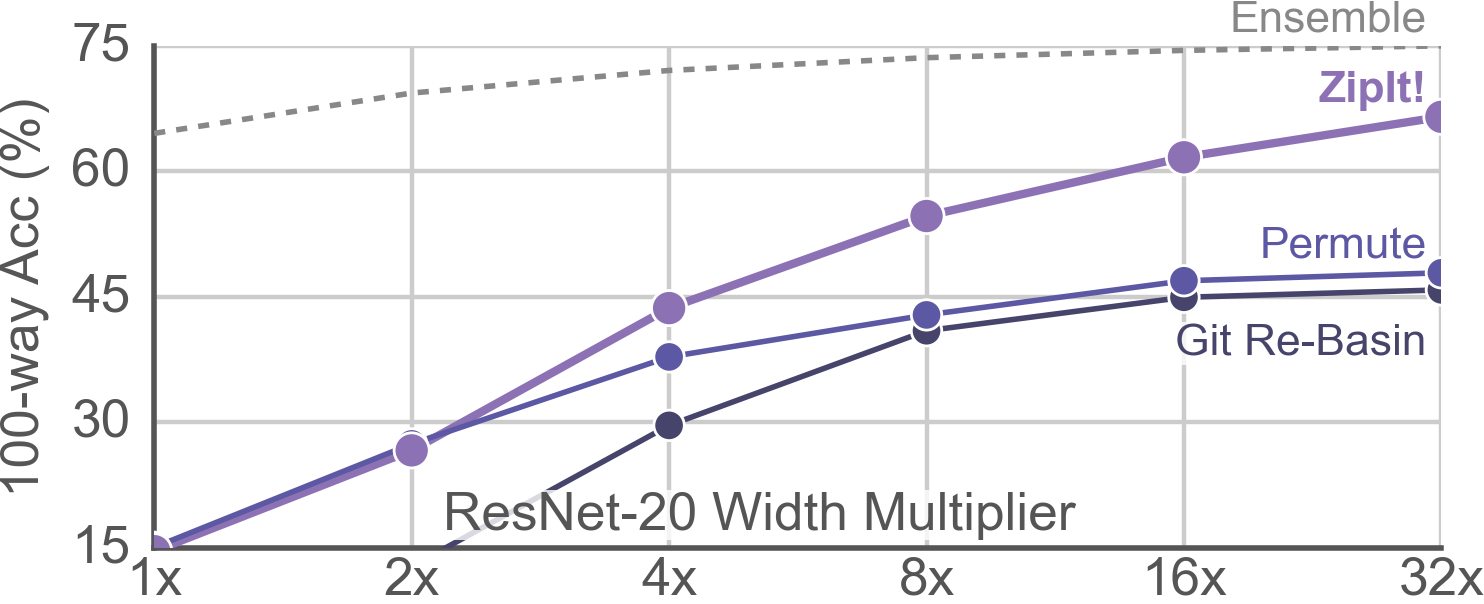
\includegraphics[width=0.95\linewidth]{figures/imgs/model_scale.png}
% \end{center}
% \caption{{\bf Model Scale.} As we increase the width of the ResNet-20 models used for the CIFAR-100 (50+50) setting, \name{}\ makes effective use of that extra capacity, quickly approaching ensemble accuracy. 
% Git Re-Basin \cite{ainsworth2022git} and Permute only slightly benefit from the extra scale.
% }
% \label{fig:model_size}
% \end{figure}


\section{Analysis} \label{sec:ablations}
% Here, we analyze and ablate the performance of \name{}\ on the settings described in Sec.~\ref{sec:results}.


\paragraph{Merging \textit{within} Models.}
A critical piece of \name{}\ compared to prior work is the ability to merge \textit{within} models, not just \textit{across} models. In Sec.~\ref{sec:partial_zip}, we introduce a budget parameter $\beta$ to limit the number of same-model merges, 
and here use CIFAR-100 (50+50) and ImageNet-1k (200+200) to illustrate its effectiveness (Fig.~\ref{fig:variations}\hyperref[fig:variations]{a}).
On CIFAR, same-model merges are very important, with the optimal budget being above 0.8, meaning 80\% of merges are allowed to be within the same model. This is not the case, however, on ImageNet, where the difficulty of the task means there likely are much fewer redundant features \textit{within} each model.

\paragraph{Model Scale.}
In Fig.~\ref{fig:variations}\hyperref[fig:variations]{b}, we test the effect of model scale directly by evaluating joint accuracy on our CIFAR-100 (50+50) setting with ResNet-20 models of increasing width. Here, we explicitly see that when the width of the models are too small for the task (e.g., $<4\times$), \name{}\ and the Permute baseline perform identically (though both much better than Git Re-Basin). However, when the scale increases, \name{}\ trends toward the ensemble upper bound of 75\%, while both the Permute baseline and Git Re-Basin plateau at around 45\%. This corroborates Eq.~\ref{eq:mainpaper_barrier} and indicates our method uses the extra model capacity effectively, much better than prior work.
\begin{wrapfigure}{r}{0.5\textwidth}
% \vspace{-10pt}
\resizebox{0.48\textwidth}{!}{
        \tablestyle{7pt}{1.05}
        \begin{tabular}{y{55}x{43}x{22}x{30}}
            Algorithm & \modela{A}$\leftrightarrow$\modela{A}/\modelb{B}$\leftrightarrow$\modelb{B}? & Acc & Time\\
            \shline
            Identity {\scriptsize (Eq.~\ref{eq:wavg})}                  & \xmark{} & {43.0\conf{3.1}} & {1.8\unit{ms}} \\
            Permute {\scriptsize (Eq.~\ref{eq:rebasin})}                & \xmark{} & {58.4\conf{1.3}} & {28\unit{ms}} \\
            K-Means                                                     & \checkmark{} & {29.1\conf{5.5}} & {19\unit{sec}} \\
            \hline
            \multicolumn{4}{c}{Zip {\scriptsize (Eq.~\ref{eq:zip})}} \\
            Optimal Match                                               & \checkmark{} & {\bf 79.6\conf{1.7}} & {11\unit{min}} \\
            Greedy Match                                                & \checkmark{} & {\bf 79.0\conf{1.8}} & {1.1\unit{sec}} \\
            Greedy, $\alpha$=0.1 & \default{\checkmark{}} & \default{\textbf{79.1\conf{2.1}}}  &  \default{1.2\unit{sec}}  \\
        \end{tabular}
    }
    \captionof{table}{{\bf Comparing Matching Algorithms} to use for \modelc{$M_i$} on CIFAR-10 (5+5) joint 10-way accuracy.
    Permuting \modelb{B}$\rightarrow$\modela{A} as in prior work (Eq.~\ref{eq:rebasin}) performs poorly. 
    We significantly improve by merging features \textit{within} each model (Eq.~\ref{eq:zip}).
    Our greedy approach is nearly as accurate as the optimal algorithm while being two orders of magnitude faster. 
    }
    \label{tab:matching_alg}
    \vspace{-10pt}
\end{wrapfigure}
% \end{table}


% \begin{wrapfigure}{l}{0.48\linewidth}
% % \vspace{-260pt}
% \begin{minipage}[l]{\linewidth}{
%     \begin{minipage}[c]{\linewidth}
%         \centering
%         \resizebox{\textwidth}{!}{
%             \tablestyle{7pt}{1.05}
%             \begin{tabular}{y{55}x{43}x{22}x{30}}
%                 Algorithm & \modela{A}$\leftrightarrow$\modela{A}/\modelb{B}$\leftrightarrow$\modelb{B}? & Acc & Time\\
%                 \shline
%                 Identity {\scriptsize (Eq.~\ref{eq:wavg})}                  & \xmark{} & {43.0\conf{3.1}} & {1.8\unit{ms}} \\
%                 Permute {\scriptsize (Eq.~\ref{eq:rebasin})}                & \xmark{} & {58.4\conf{1.3}} & {28\unit{ms}} \\
%                 K-Means                                                     & \checkmark{} & {29.1\conf{5.5}} & {19\unit{sec}} \\
%                 \hline
%                 \multicolumn{4}{c}{Zip {\scriptsize (Eq.~\ref{eq:zip})}} \\
%                 Optimal Match                                               & \checkmark{} & {\bf 79.6\conf{1.7}} & {11\unit{min}} \\
%                 Greedy Match                                                & \checkmark{} & {\bf 79.0\conf{1.8}} & {1.1\unit{sec}} \\
%                 Greedy, $\alpha$=0.1 & \default{\checkmark{}} & \default{\textbf{79.1\conf{2.1}}}  &  \default{1.2\unit{sec}}  \\
%             \end{tabular}
%         }
%         \captionof{table}{{\bf Matching Algorithm} to use for \modelc{$M_i$}. 
%         Permuting \modelb{B}$\rightarrow$\modela{A} as in prior work (Eq.~\ref{eq:rebasin}) performs poorly, thus we allow merging features \textit{within} each model (Eq.~\ref{eq:zip}).
%         Our greedy approach is nearly as accurate as the optimal algorithm while being two orders of magnitude faster. 
%         ``Acc'' is CIFAR-10 (5+5) joint 10-way accuracy.
%         }
%         \label{tab:matching_alg}
%     \end{minipage}
%     \vspace{10pt}
%     \begin{minipage}[c]{\linewidth}
%         % \vspace{40pt}
%         \centering
%         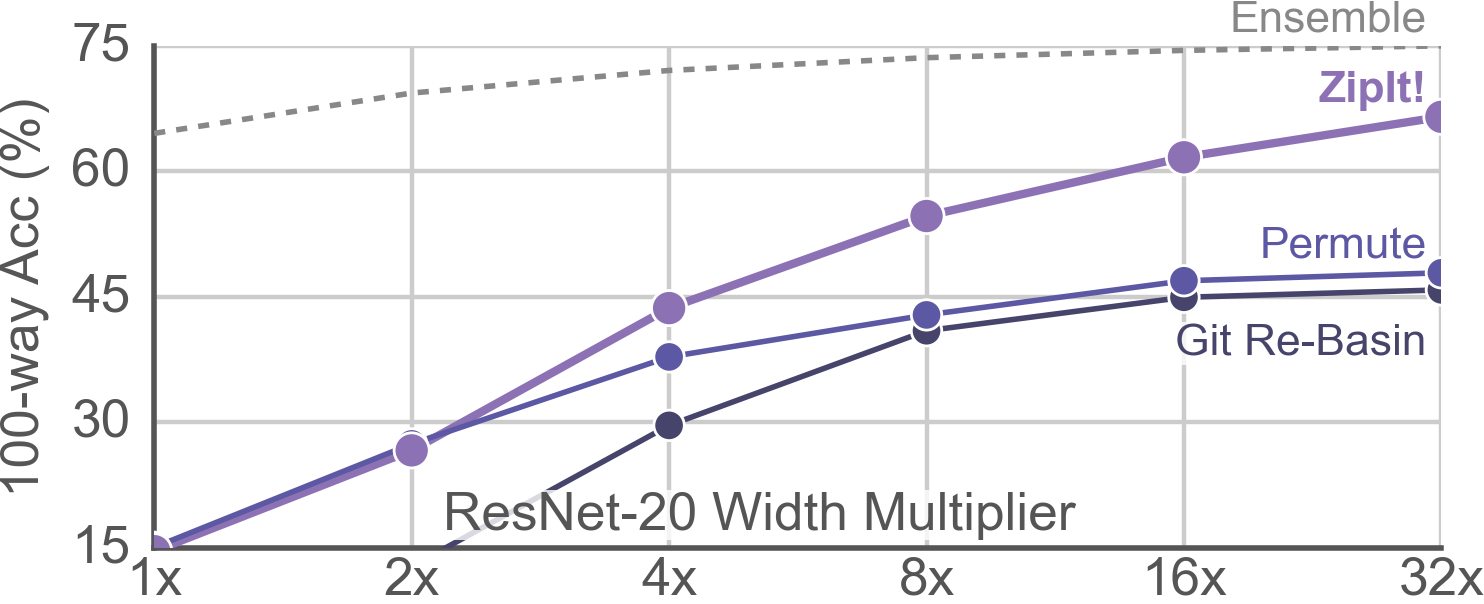
\includegraphics[width=0.95\linewidth]{figures/imgs/model_scale.png}
%         \caption{{\bf Model Scale.} 
%         \name{}\ makes effective use of extra model capacity to quickly reach the ensemble on CIFAR-100 (50+50) when we increase the width of ResNet-20 models.
%         % \name{}\ quickly approaches ensemble accuracy as we increase the width of the ResNet-20 models in the CIFAR-100 (50+50) setting, making effective use of extra capacity from scale.
%         % As we increase the width of the ResNet-20 models used for the CIFAR-100 (50+50) setting, \name{}\ makes effective use of that extra capacity, quickly approaching ensemble accuracy. 
%         Git Re-Basin \cite{ainsworth2022git} and Permute only slightly benefit from the extra scale.
%         }
%         \label{fig:model_size}
%         \vspace{-30pt}
%     \end{minipage}
% }\end{minipage}
% \end{wrapfigure}










% \begin{table}[t]
% \centering

% \tablestyle{7pt}{1.05}
% \begin{tabular}{y{50}x{43}x{22}x{30}}
%     Algorithm & \modela{A}$\leftrightarrow$\modela{A}/\modelb{B}$\leftrightarrow$\modelb{B}? & Acc & Time\\
%     \shline
%     Identity {\scriptsize (Eq.~\ref{eq:wavg})}                  & \xmark{} & {43.0\conf{3.1}} & {1.8\unit{ms}} \\
%     Permute {\scriptsize (Eq.~\ref{eq:rebasin})}                & \xmark{} & {58.4\conf{1.3}} & {28\unit{ms}} \\
%     K-Means                                                     & \checkmark{} & {29.1\conf{5.5}} & {19\unit{sec}} \\
%     \hline
%     \multicolumn{4}{c}{Zip {\scriptsize (Eq.~\ref{eq:zip})}} \\
%     Optimal Match                                               & \checkmark{} & {\bf 79.6\conf{1.7}} & {11\unit{min}} \\
%     Greedy Match                                                & \checkmark{} & {\bf 79.0\conf{1.8}} & {1.1\unit{sec}} \\
%     Greedy, $\alpha$=0.1 & \default{\checkmark{}} & \default{\textbf{79.1\conf{2.1}}}  &  \default{1.2\unit{sec}}  \\
% \end{tabular}
% \caption{{\bf Matching Algorithm} to use for \modelc{$M_i$}. 
% Permuting \modelb{B}$\rightarrow$\modela{A} as in prior work (Eq.~\ref{eq:rebasin}) performs poorly, thus we allow merging features \textit{within} each model (Eq.~\ref{eq:zip}).
% Our greedy approach is nearly as accurate as the optimal algorithm while being two orders of magnitude faster. 
% ``Acc'' is CIFAR-10 (5+5) joint 10-way accuracy.
% }
% \label{tab:matching_alg}
% \end{table}

\vspace{-1em}
\paragraph{Matching Algorithm.}
In Tab.~\ref{tab:matching_alg}, we compare matching algorithms used to compute \modelc{$M_i$} in Eq.~\ref{eq:zip}. Using either the identity (weight averaging) or a permutation (as in prior work) underperforms on CIFAR-10 (5+5) joint 10-way classification. 
In contrast, we obtain up to 21.2\% higher accuracy if we allow both permutations and \textit{merging within models}.
% In contrast, if we allow merging \textit{within} models as well, then we obtain up to 21.2\% higher accuracy than permuting alone. 
However, doing this optimally is difficult, as the standard linear sum assignment algorithm assumes bipartite matches. We could use a optimal graph-based solver (e.g., \citet{networkx}) instead, but doing so is prohibitively slow (11 minutes to transform a ResNet-20$\times$4 model). Thus, we find matches greedily by repeatedly taking the most correlated pair of features without replacement. This performs almost as well, and is multiple orders of magnitude faster. If we allow repeated matches (Sec.~\ref{sec:partial_zip}), we obtain a slightly better result.
Like \citet{bolya2022token}, we find that matching is better for merging features than clustering (K-Means).

% % \begin{wrapfigure}{l}{0.48\linewidth}
% % \begin{figure}[t]
% \centering
% %
% \begin{center}
%     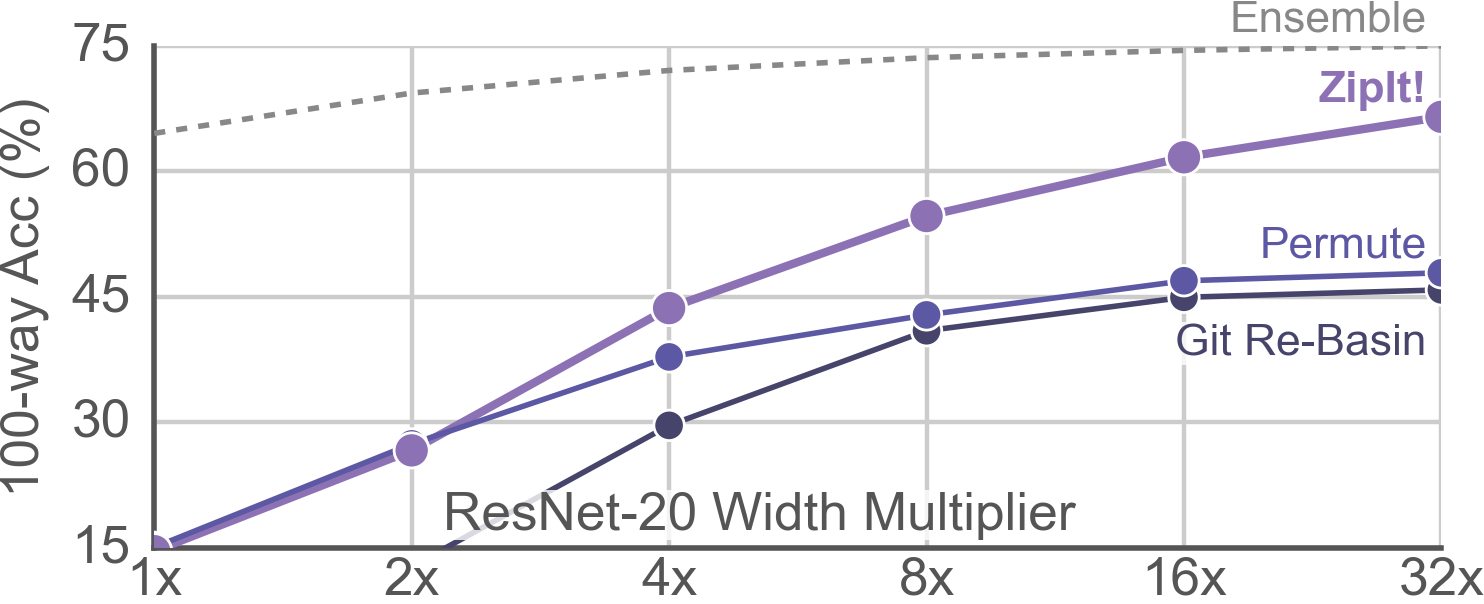
\includegraphics[width=0.95\linewidth]{figures/imgs/model_scale.png}
% \end{center}
% \caption{{\bf Model Scale.} As we increase the width of the ResNet-20 models used for the CIFAR-100 (50+50) setting, \name{}\ makes effective use of that extra capacity, quickly approaching ensemble accuracy. 
% Git Re-Basin \cite{ainsworth2022git} and Permute only slightly benefit from the extra scale.
% }
% \label{fig:model_size}
% \end{wrapfigure}
% % \end{figure}
% indicates that our method uses the extra capacity of these models effectively, much better than prior work.

% % \begin{figure}[t]
% \centering

% \subfloat[
%     \textbf{CIFAR-100 50+50.}
%     \label{fig:partial_zip_cifar100}
% ]{
% \centering
% \begin{minipage}{0.49\linewidth}{
% \begin{center}
%     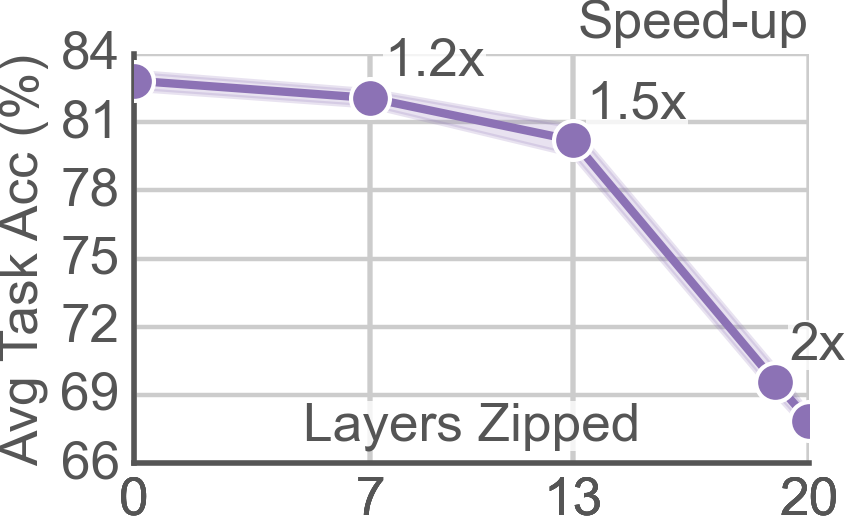
\includegraphics[width=\linewidth]{figures/imgs/partial_zip_CIFAR_50_50.png}
% \end{center}
% }\end{minipage}
% }
% \subfloat[
%     \textbf{ImageNet-1k 200+200.}
%     \label{fig:partial_zip_imagenet}
% ]{
% \centering
% \begin{minipage}{0.49\linewidth}{
% \begin{center}
%     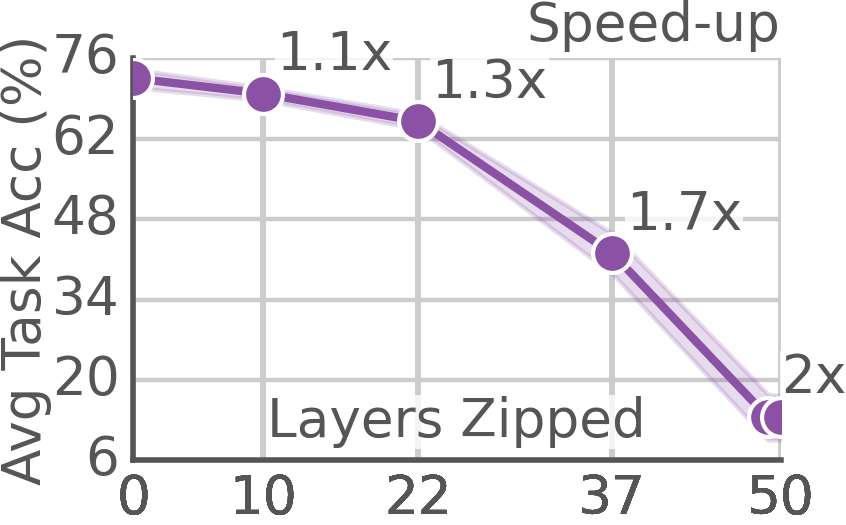
\includegraphics[width=\linewidth]{figures/imgs/partial_zip_imnet_200_200.png}
% \end{center}
% }\end{minipage}
% }

% \caption{
% {\bf Varying Partial Zip.} 
% By leaving some layers unzipped (Sec.~\ref{sec:partial_zip}), we can recover a significant amount of performance while still merging most of the model. 
% }
% \label{fig:varying_partial_zip}
% \end{figure}

% \begin{wrapfigure}{r}{0.48\linewidth}
% \vspace{-10pt}
% \centering
% \resizebox{\linewidth}{!}{
%     \tablestyle{5pt}{1.1}
%     {
%     \tablestyle{5pt}{1.1}
%     \begin{tabular}{x{40}x{40}x{40}}
%         \multicolumn{3}{c}{Average Stage Correlations}\\
%         Layer \sfrac{7}{20} & Layer \sfrac{13}{20} & Layer \sfrac{19}{20}\\
%     \shline
%     {0.50\conf{0.01}} & {0.37\conf{0.00}} & {0.27\conf{0.00}} \\
%     \hline
% \end{tabular}
%     }
% }
% \captionof{table}{\textbf{CIFAR-100 (50+50) Zipping Correlations.} We show the average correlations between two ResNet-20 ($8\times$) models at each partial zipping stage. Correlations consistently decrease at each successive stage, indicating that the layers of the two models increasingly diverge. 
% }
% \label{tab:partialzip_corrs}
% % \end{table}
% \vspace{-20pt}
% \end{wrapfigure}


\begin{wrapfigure}{r}{0.48\linewidth}
\vspace{-15pt}
\begin{minipage}[l]{\linewidth}{
\captionsetup{justification=centering}
\subfloat[
    \textbf{CIFAR-100 \\ \ \ \ \ (50+50)}
    \label{fig:partial_zip_cifar100}
]{
\centering
\begin{minipage}{0.48\linewidth}{
\begin{center}
    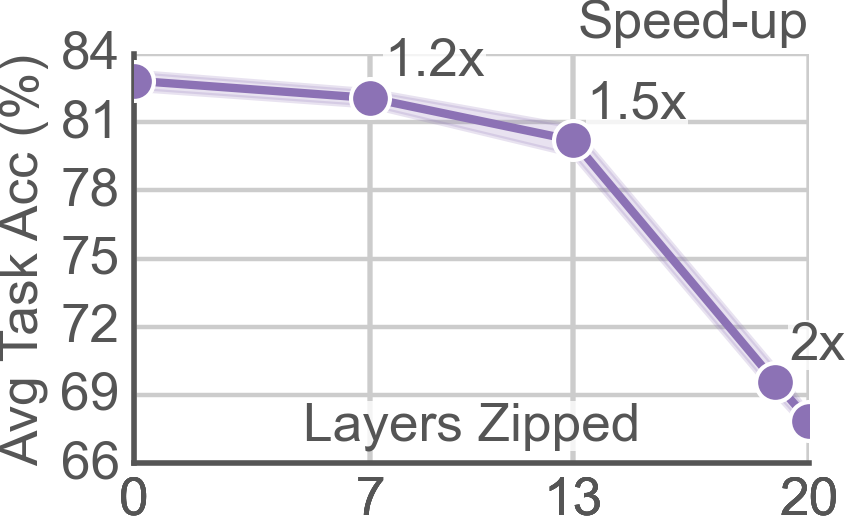
\includegraphics[width=\linewidth]{figures/imgs/partial_zip_CIFAR_50_50.png}
\end{center}
}\end{minipage}
}
\subfloat[
    \textbf{ImageNet-1k \\ \ \ \  (200+200)}
    \label{fig:partial_zip_imagenet}
]{
\centering
\begin{minipage}{0.48\linewidth}{
\begin{center}
    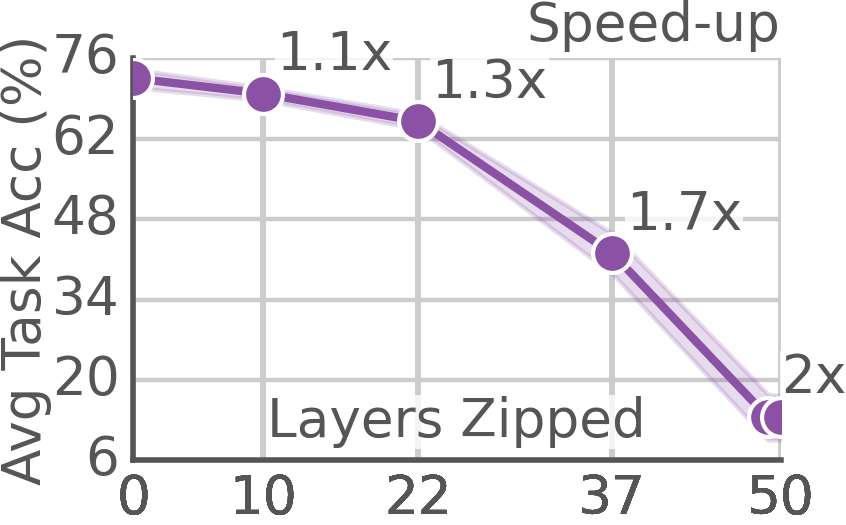
\includegraphics[width=\linewidth]{figures/imgs/partial_zip_imnet_200_200.png}
\end{center}
}\end{minipage}
}
\captionsetup{justification=justified}
        \caption{{\bf Varying Partial Zip.} By leaving some layers unzipped (Sec.~\ref{sec:partial_zip}), we can recover a significant amount of performance while still merging most of the model. }
\label{fig:varying_partial_zip}
}\end{minipage}
\begin{minipage}[l]{\linewidth}{
\vspace{5pt}
\centering
\resizebox{\linewidth}{!}{
    \tablestyle{5pt}{1.1}
    {
    \tablestyle{5pt}{1.1}
    \begin{tabular}{x{40}x{40}x{40}}
        \multicolumn{3}{c}{Average Stage Correlations}\\
        Layer \sfrac{7}{20} & Layer \sfrac{13}{20} & Layer \sfrac{19}{20}\\
    \shline
    {0.50\conf{0.01}} & {0.37\conf{0.00}} & {0.27\conf{0.00}} \\
    \hline
\end{tabular}
    }
}
\captionof{table}{\textbf{CIFAR-100 (50+50) Zipping Correlations.} We show the average correlations between two ResNet-20 ($8\times$ width) models at each partial zipping stage. Correlations consistently decrease at each successive stage, indicating that the layers of the two models increasingly diverge. 
}
\label{tab:partialzip_corrs}
% \end{table}
% \vspace{10pt}
}\end{minipage}
\begin{minipage}[l]{\linewidth}{
\captionsetup{justification=centering}
\vspace{1em}
\subfloat[
    \textbf{CIFAR-100 \\ \ \ \ \ (50+50)}
    \label{fig:data_use_cifar100}
]{
\centering
\begin{minipage}{0.48\linewidth}{
\begin{center}
    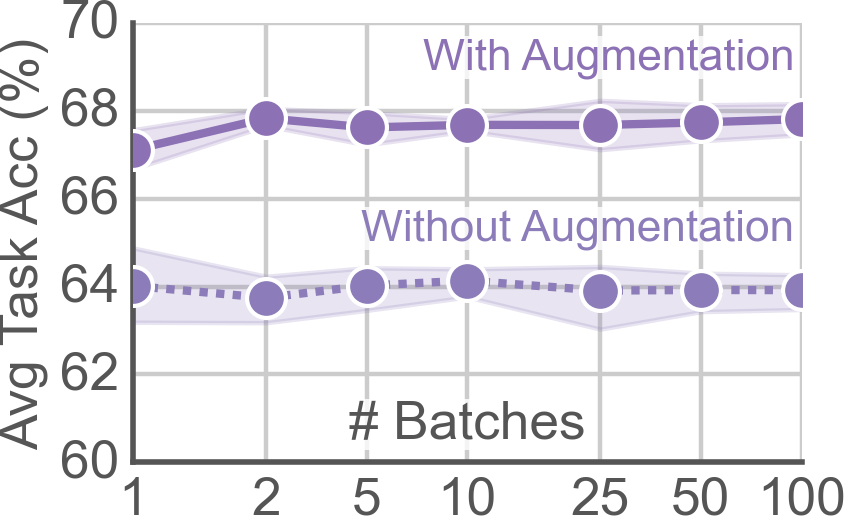
\includegraphics[width=\linewidth]{figures/imgs/cifar100_data.png}
\end{center}
}\end{minipage}
}
\subfloat[
    \textbf{ImageNet-1k \\ \ \ \  (200+200)}
    \label{fig:data_use_imagenet}
]{
\centering
\begin{minipage}{0.48\linewidth}{
\begin{center}
    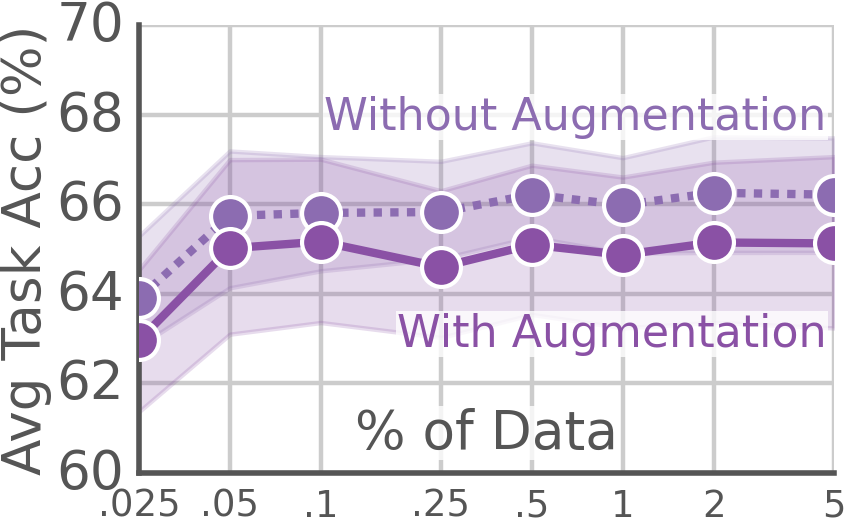
\includegraphics[width=\linewidth]{figures/imgs/imnet200_data.png}
\end{center}
}\end{minipage}
}
\captionsetup{justification=justified}
\caption{
{\bf Data Usage.} 
How much data do we need to use to compute activations? 
We find that only a few hundred images are needed to obtain the best performance.
Data augmentation is not always useful.
% Here we ablate the amount of data used for our CIFAR-100 (50+50) ResNet-20 ($8\times$ width) and ImageNet (200+200) Resnet-50 (\sfrac{22}{50} layers) experiments. 
% The batch size used is 500 for CIFAR and 16 for ImageNet. 
% In both cases, we only need a few hundred images to obtain the best results. 
% On the other hand, data augmentation is necessary for CIFAR but hurts for ImageNet. Our default for all experiments uses data augmentation and the full set for CIFAR (100 batches) and 1\% of the data for ImageNet. 
}
\label{fig:data_usage}
}\end{minipage}
% \vspace{-60pt}
\end{wrapfigure}

% \begin{wrapfigure}{l}{0.52\linewidth}
% % \vspace{-260pt}
% \begin{minipage}[l]{\linewidth}{
% \subfloat[
%     \textbf{CIFAR-100 (50+50).}
%     \label{fig:data_use_cifar100}
% ]{
% \centering
% \begin{minipage}{0.48\linewidth}{
% \begin{center}
%     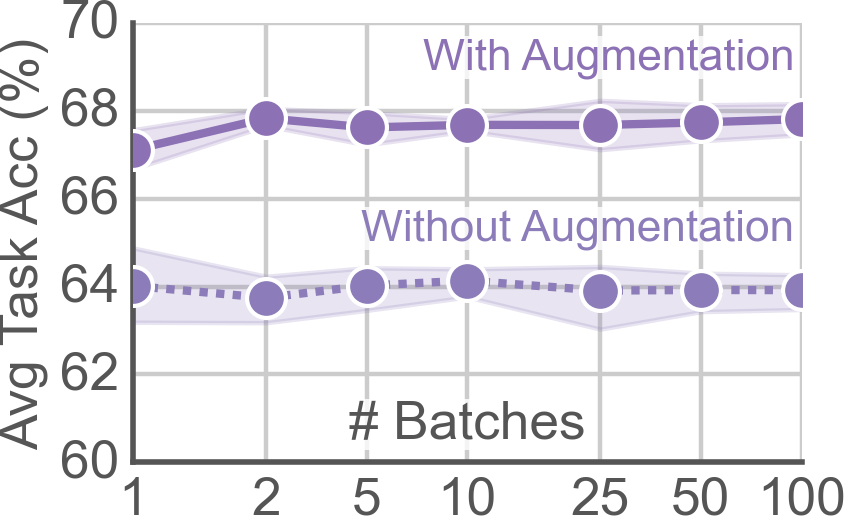
\includegraphics[width=\linewidth]{figures/imgs/cifar100_data.png}
% \end{center}
% }\end{minipage}
% }
% \subfloat[
%     \textbf{ImageNet-1k (200+200).}
%     \label{fig:data_use_imagenet}
% ]{
% \centering
% \begin{minipage}{0.48\linewidth}{
% \begin{center}
%     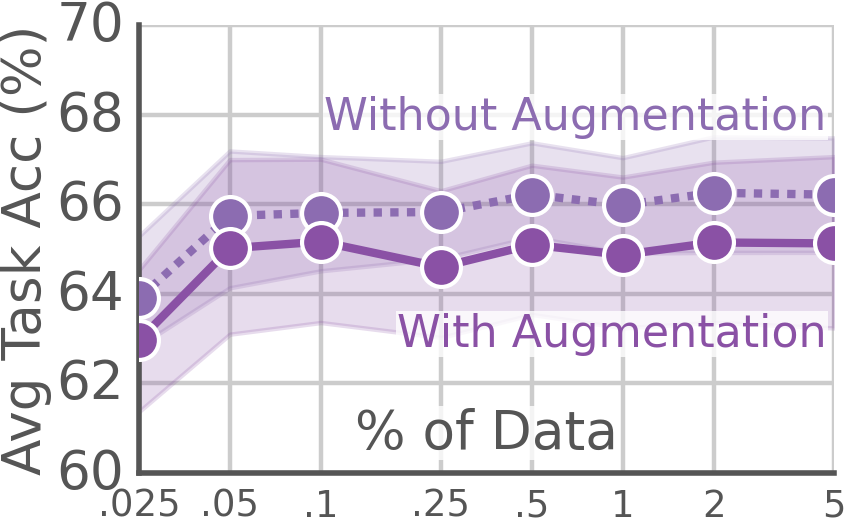
\includegraphics[width=\linewidth]{figures/imgs/imnet200_data.png}
% \end{center}
% }\end{minipage}
% }
%         \caption{
%         {\bf Data Usage.} How much data do we need to use to compute activations? Here we ablate the amount of data used for our CIFAR-100 (50+50) ResNet-20 ($8\times$ width) and ImageNet (200+200) Resnet-50 (\sfrac{22}{50} layers) experiments. The batch size used is 500 for CIFAR and 16 for ImageNet. In both cases, we only need a few hundred images to obtain the best results. On the other hand, data augmentation is necessary for CIFAR but hurts for ImageNet. Our default for all experiments uses data augmentation and the full set for CIFAR (100 batches) and 1\% of the data for ImageNet. 
%         }
% \label{fig:data_usage}
% }\end{minipage}
% \end{wrapfigure}


% \caption{{\bf Data Usage.} How much data do we need to use to compute activations? Here we ablate the amount of data used for our CIFAR-100 (50+50) ResNet-20 ($8\times$ width) and ImageNet (200+200) Resnet-50 (\sfrac{22}{50} layers) experiments. The batch size used is 500 for CIFAR and 16 for ImageNet. In both cases, we only need a few hundred images to obtain the best results. On the other hand, data augmentation is necessary for CIFAR but hurts for ImageNet. Our default for all experiments uses data augmentation and the full set for CIFAR (100 batches) and 1\% of the data for ImageNet. }
% \label{fig:data_usage}
% \end{figure}


% \begin{figure}
%     \begin{minipage}[t]{0.50\linewidth}
%         \centering
%         \subfloat[
%             \textbf{CIFAR-100 (50+50).}
%             \label{fig:partial_zip_cifar100}
%         ]{
%             \centering
%             \begin{minipage}{0.40\linewidth}{
%                 \centering
%                 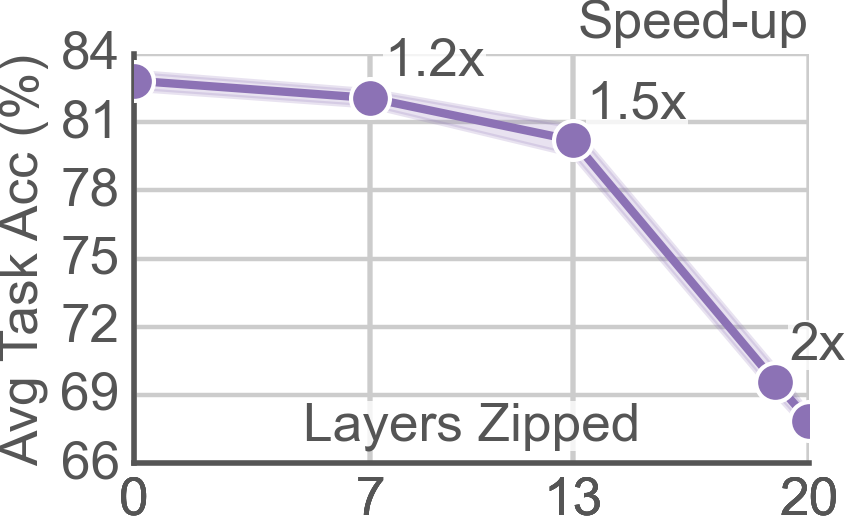
\includegraphics[width=\linewidth]{figures/imgs/partial_zip_CIFAR_50_50.png}
%             }\end{minipage}
%         }
%         \subfloat[
%             \textbf{ImageNet-1k (200+200).}
%             \label{fig:partial_zip_imagenet}
%         ]{
%             \centering
%             \begin{minipage}{0.40\linewidth}{
%                 \centering
%                 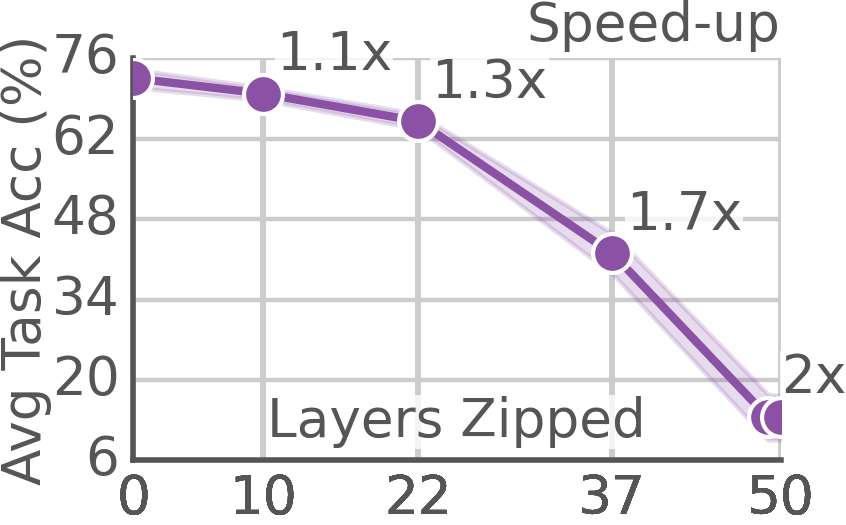
\includegraphics[width=\linewidth]{figures/imgs/partial_zip_imnet_200_200.png}
%             }\end{minipage}
%         }
%         \caption{{\bf Varying Partial Zip.} 
%             By leaving some layers unzipped (Sec.~\ref{sec:partial_zip}), we can recover a significant amount of performance while still merging most of the model.  }
%         \label{fig:varying_partial_zip}
%         % \vspace{-80pt}
%     \end{minipage}
%     \hspace{1pt}
%     % \vspace{1em} % Add vertical space between the images
%     \begin{minipage}[t]{0.48\linewidth}
%         \centering
%         \subfloat[
%             \textbf{CIFAR-100 (50+50).}
%             \label{fig:data_use_cifar100}
%         ]{
%             \centering
%             \begin{minipage}{0.48\linewidth}{
%                 \centering
%                 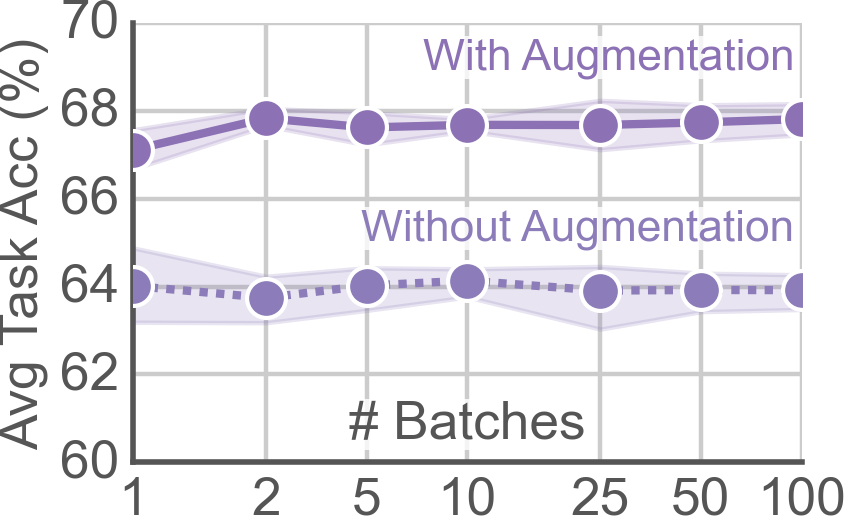
\includegraphics[width=\linewidth]{figures/imgs/cifar100_data.png}
%             }\end{minipage}
%         }
%         \subfloat[
%             \textbf{ImageNet-1k (200+200).}
%             \label{fig:data_use_imagenet}
%         ]{
%             \centering
%             \begin{minipage}{0.48\linewidth}{
%                 \centering
%                 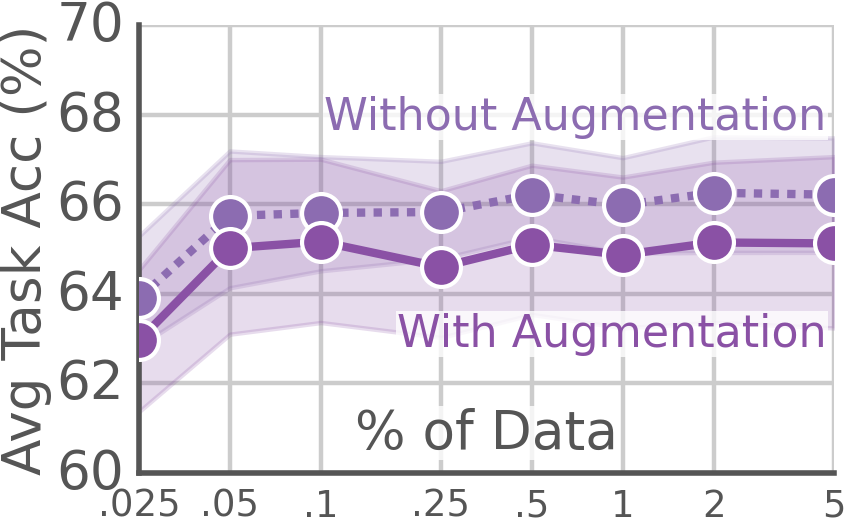
\includegraphics[width=\linewidth]{figures/imgs/imnet200_data.png}
%             }\end{minipage}
%         }
%         \caption{
%         {\bf Data Usage.} How much data do we need to use to compute activations? Here we ablate the amount of data used for our CIFAR-100 (50+50) ResNet-20 ($8\times$ width) and ImageNet (200+200) Resnet-50 (\sfrac{22}{50} layers) experiments. The batch size used is 500 for CIFAR and 16 for ImageNet. In both cases, we only need a few hundred images to obtain the best results. On the other hand, data augmentation is necessary for CIFAR but hurts for ImageNet. Our default for all experiments uses data augmentation and the full set for CIFAR (100 batches) and 1\% of the data for ImageNet. 
%         }
%         \label{fig:data_usage}
%         % \vspace{10pt}
%     \end{minipage}
%     % \caption{Overall caption for the three images}
%     \vspace{-20pt}
% \end{figure}

% \paragraph{Partial Zipping.} Overall, we find partial zipping to be a simple yet effective technique to add capacity back to the merged model. For CIFAR-100, we can obtain near ensemble accuracies at a 1.5$\times$ speed-up (Tab.~\ref{tab:cifar50+50}). Similarly on a difficult setting like ImageNet, partial zipping is \textit{necessary} to obtain any reasonable accuracy. Additional results in Appendix~\ref{ap:partial_zipping}.

% In Fig.~\ref{fig:variations}, we plot the average per task accuracy by the number of layers zipped in ResNet-20$\times$8 for CIFAR-100 (50+50) and ResNet-50 for ImageNet-1k (200+200). Note that to avoid adding extra unmerge modules into the network, our stopping point while unzipping has to be the end of a stage. 
% Overall, we find partial zipping to be a simple yet effective technique to add capacity back to the merged model. For CIFAR-100, we can obtain near ensemble accuracies at a 1.5$\times$ speed-up. Similarly on a difficult setting like ImageNet, partial zipping is \textit{necessary} to obtain any reasonable accuracy.

% \vspace{-0.5em}
\section{Conclusion}
% \vspace{-0.4em}
In this paper, we tackle the extremely difficult task of merging models trained on completely disjoint tasks \textit{without additional training}.
We find that prior work underperforms in this setting and posit that they neither fully (1) exploit model similarities nor (2) account for model dissimilarities.
We introduce \name{}, a general framework for merging models that addresses these issues, and show it to significantly outperform prior work across several difficult settings, comprehensively analyzing each.
% We hope \name{}\ can serve as a strong starting point for practical applications of merging models trained on different tasks.


% In this paper, we tackle the extremely difficult task of merging models trained on completely disjoint tasks \textit{without additional training}.
% We show experimentally how prior work falls short in this setting and posit that this is due to not merging features \textit{within models} as well as merging \textit{every} layer in the model at once. 
% We then introduce \name{}, a generalized framework for merging models that deals with these issues and find it to significantly outperform both prior work \cite{ainsworth2022git} and our own strong baseline on a number of difficult model merging settings. 
% We then analyze the behavior of our method and find that at smaller model capacities, it performs similarly to permutation-based methods, but can perform much better as the model capacity increases.
% We hope \name{}\ can serve as a strong starting point for practical applications of merging models trained on different tasks.

\paragraph{Reproducibility Statement.}
To ensure reproducibility, we will release code for our algorithm, experiments, and baselines. We also include algorithm details in Section~\ref{sec:approach} and further in Appendix~\ref{ap:prop_rules}, experimental details in Section~\ref{sec:results} and Appendix~\ref{ap:data_usage}, and a proof of our Theorem~\hyperref[ap:TheoremDef]{1} in Appendix~\ref{ap:Theorem}.

\paragraph{Acknowledgements.}
This work was supported in part by funding from NSF CAREER \#2144194, ARL, Google, and NSF GRFP. All views and conclusions expressed in this work are those of the authors and not a reflection of these sources.

\bibliography{main}
\bibliographystyle{template/iclr2024_conference}
\clearpage
\appendix
\section{Partial Zipping}\label{ap:partial_zipping}
In Fig.~\ref{fig:varying_partial_zip} we plot the average per task accuracy by the number of layers zipped in ResNet-20$\times$8 for CIFAR-100 (50+50) and ResNet-50 for ImageNet-1k (200+200). 
Note that to avoid adding extra unmerge modules into the network, our stopping point while unzipping has to be the end of a stage. 

In Table~\ref{tab:partialzip_corrs}, we show the average neuron correlations at each partial-zipping stage between the layers of ResNet-20 ($8\times$) models trained on the CIFAR-100 (50+50) task. 
We collect results using the same models used in Table \ref{tab:cifar50+50}, and compute correlations as described in Section \ref{sec:approach}.
Overall, we find the correlations between models consistently decreases through successive partial zipping locations. 
This corroborates the finding of \citet{kornblith2019similarity} that model layers become increasingly dissimilar with depth, as they encode more task-specific features. 
Coupling Table \ref{tab:partialzip_corrs} with Figure \ref{fig:partial_zip_cifar100}, we observe a direct correlation between layer-(dis)similarities and performance decrease.
This illustrates the importance of layer similarity between two networks and strong performance.
% \begin{figure}[t]
% \centering

% \subfloat[
%     \textbf{CIFAR-100 50+50.}
%     \label{fig:partial_zip_cifar100}
% ]{
% \centering
% \begin{minipage}{0.49\linewidth}{
% \begin{center}
%     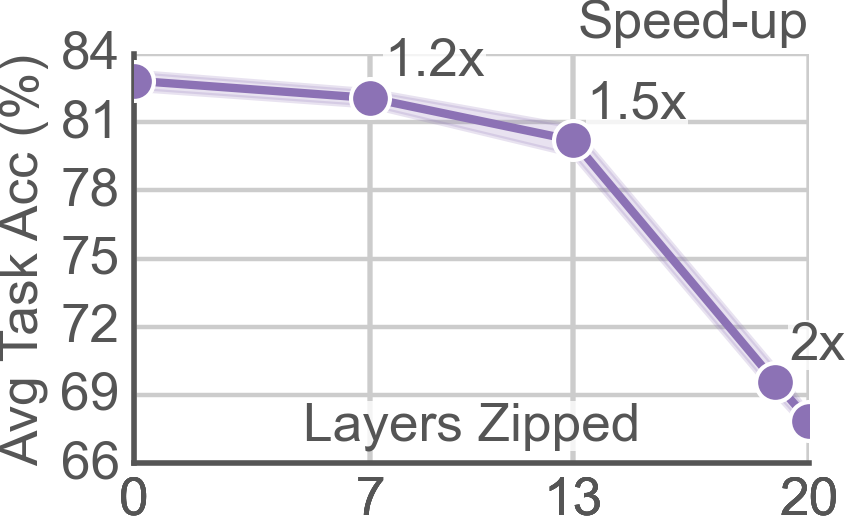
\includegraphics[width=\linewidth]{figures/imgs/partial_zip_CIFAR_50_50.png}
% \end{center}
% }\end{minipage}
% }
% \subfloat[
%     \textbf{ImageNet-1k 200+200.}
%     \label{fig:partial_zip_imagenet}
% ]{
% \centering
% \begin{minipage}{0.49\linewidth}{
% \begin{center}
%     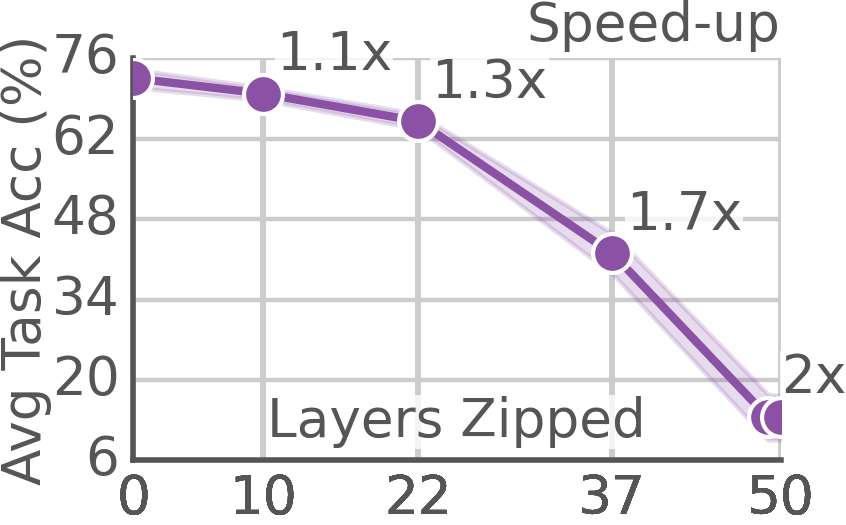
\includegraphics[width=\linewidth]{figures/imgs/partial_zip_imnet_200_200.png}
% \end{center}
% }\end{minipage}
% }

% \caption{
% {\bf Varying Partial Zip.} 
% By leaving some layers unzipped (Sec.~\ref{sec:partial_zip}), we can recover a significant amount of performance while still merging most of the model. 
% }
% \label{fig:varying_partial_zip}
% \end{figure}

% \begin{wrapfigure}{r}{0.48\linewidth}
% \vspace{-10pt}
% \centering
% \resizebox{\linewidth}{!}{
%     \tablestyle{5pt}{1.1}
%     {
%     \tablestyle{5pt}{1.1}
%     \begin{tabular}{x{40}x{40}x{40}}
%         \multicolumn{3}{c}{Average Stage Correlations}\\
%         Layer \sfrac{7}{20} & Layer \sfrac{13}{20} & Layer \sfrac{19}{20}\\
%     \shline
%     {0.50\conf{0.01}} & {0.37\conf{0.00}} & {0.27\conf{0.00}} \\
%     \hline
% \end{tabular}
%     }
% }
% \captionof{table}{\textbf{CIFAR-100 (50+50) Zipping Correlations.} We show the average correlations between two ResNet-20 ($8\times$) models at each partial zipping stage. Correlations consistently decrease at each successive stage, indicating that the layers of the two models increasingly diverge. 
% }
% \label{tab:partialzip_corrs}
% % \end{table}
% \vspace{-20pt}
% \end{wrapfigure}


\begin{wrapfigure}{r}{0.48\linewidth}
\vspace{-15pt}
\begin{minipage}[l]{\linewidth}{
\captionsetup{justification=centering}
\subfloat[
    \textbf{CIFAR-100 \\ \ \ \ \ (50+50)}
    \label{fig:partial_zip_cifar100}
]{
\centering
\begin{minipage}{0.48\linewidth}{
\begin{center}
    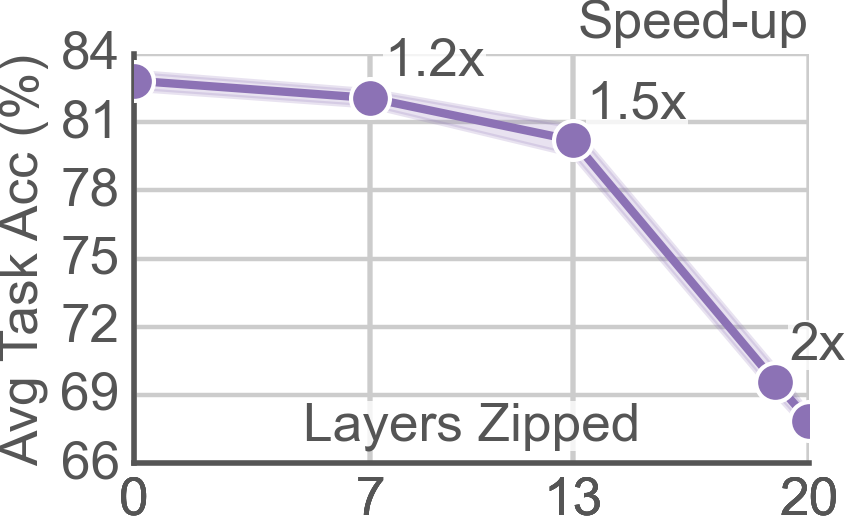
\includegraphics[width=\linewidth]{figures/imgs/partial_zip_CIFAR_50_50.png}
\end{center}
}\end{minipage}
}
\subfloat[
    \textbf{ImageNet-1k \\ \ \ \  (200+200)}
    \label{fig:partial_zip_imagenet}
]{
\centering
\begin{minipage}{0.48\linewidth}{
\begin{center}
    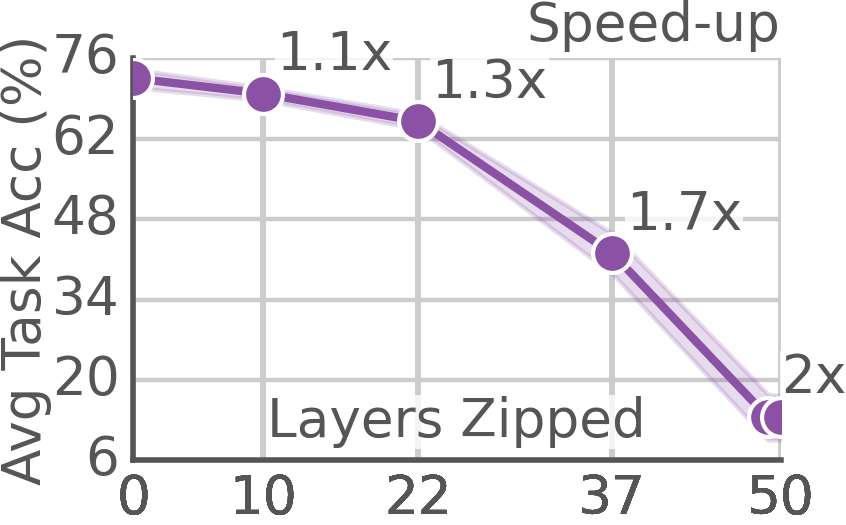
\includegraphics[width=\linewidth]{figures/imgs/partial_zip_imnet_200_200.png}
\end{center}
}\end{minipage}
}
\captionsetup{justification=justified}
        \caption{{\bf Varying Partial Zip.} By leaving some layers unzipped (Sec.~\ref{sec:partial_zip}), we can recover a significant amount of performance while still merging most of the model. }
\label{fig:varying_partial_zip}
}\end{minipage}
\begin{minipage}[l]{\linewidth}{
\vspace{5pt}
\centering
\resizebox{\linewidth}{!}{
    \tablestyle{5pt}{1.1}
    {
    \tablestyle{5pt}{1.1}
    \begin{tabular}{x{40}x{40}x{40}}
        \multicolumn{3}{c}{Average Stage Correlations}\\
        Layer \sfrac{7}{20} & Layer \sfrac{13}{20} & Layer \sfrac{19}{20}\\
    \shline
    {0.50\conf{0.01}} & {0.37\conf{0.00}} & {0.27\conf{0.00}} \\
    \hline
\end{tabular}
    }
}
\captionof{table}{\textbf{CIFAR-100 (50+50) Zipping Correlations.} We show the average correlations between two ResNet-20 ($8\times$ width) models at each partial zipping stage. Correlations consistently decrease at each successive stage, indicating that the layers of the two models increasingly diverge. 
}
\label{tab:partialzip_corrs}
% \end{table}
% \vspace{10pt}
}\end{minipage}
\begin{minipage}[l]{\linewidth}{
\captionsetup{justification=centering}
\vspace{1em}
\subfloat[
    \textbf{CIFAR-100 \\ \ \ \ \ (50+50)}
    \label{fig:data_use_cifar100}
]{
\centering
\begin{minipage}{0.48\linewidth}{
\begin{center}
    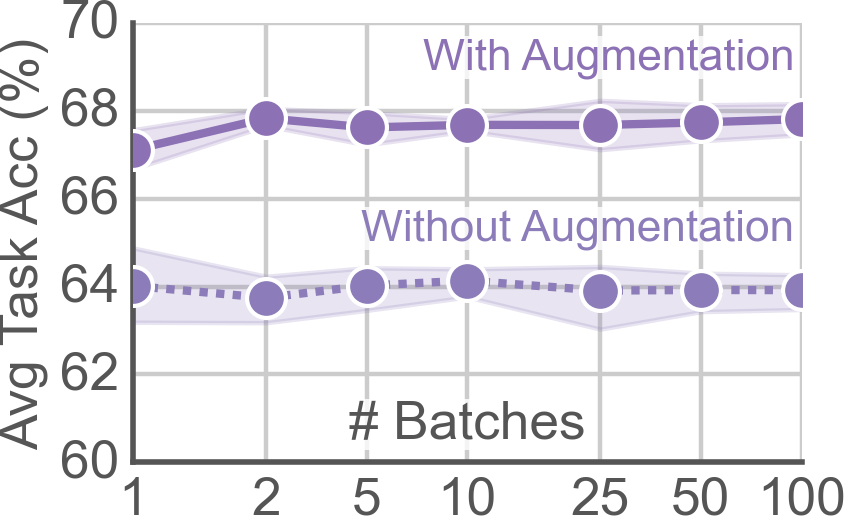
\includegraphics[width=\linewidth]{figures/imgs/cifar100_data.png}
\end{center}
}\end{minipage}
}
\subfloat[
    \textbf{ImageNet-1k \\ \ \ \  (200+200)}
    \label{fig:data_use_imagenet}
]{
\centering
\begin{minipage}{0.48\linewidth}{
\begin{center}
    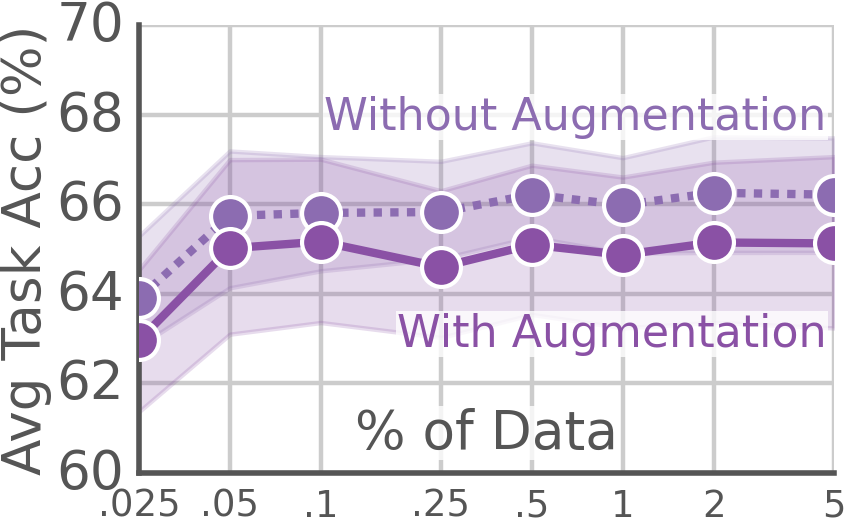
\includegraphics[width=\linewidth]{figures/imgs/imnet200_data.png}
\end{center}
}\end{minipage}
}
\captionsetup{justification=justified}
\caption{
{\bf Data Usage.} 
How much data do we need to use to compute activations? 
We find that only a few hundred images are needed to obtain the best performance.
Data augmentation is not always useful.
% Here we ablate the amount of data used for our CIFAR-100 (50+50) ResNet-20 ($8\times$ width) and ImageNet (200+200) Resnet-50 (\sfrac{22}{50} layers) experiments. 
% The batch size used is 500 for CIFAR and 16 for ImageNet. 
% In both cases, we only need a few hundred images to obtain the best results. 
% On the other hand, data augmentation is necessary for CIFAR but hurts for ImageNet. Our default for all experiments uses data augmentation and the full set for CIFAR (100 batches) and 1\% of the data for ImageNet. 
}
\label{fig:data_usage}
}\end{minipage}
% \vspace{-60pt}
\end{wrapfigure}

% \begin{wrapfigure}{l}{0.52\linewidth}
% % \vspace{-260pt}
% \begin{minipage}[l]{\linewidth}{
% \subfloat[
%     \textbf{CIFAR-100 (50+50).}
%     \label{fig:data_use_cifar100}
% ]{
% \centering
% \begin{minipage}{0.48\linewidth}{
% \begin{center}
%     \includegraphics[width=\linewidth]{figures/imgs/cifar100_data.png}
% \end{center}
% }\end{minipage}
% }
% \subfloat[
%     \textbf{ImageNet-1k (200+200).}
%     \label{fig:data_use_imagenet}
% ]{
% \centering
% \begin{minipage}{0.48\linewidth}{
% \begin{center}
%     \includegraphics[width=\linewidth]{figures/imgs/imnet200_data.png}
% \end{center}
% }\end{minipage}
% }
%         \caption{
%         {\bf Data Usage.} How much data do we need to use to compute activations? Here we ablate the amount of data used for our CIFAR-100 (50+50) ResNet-20 ($8\times$ width) and ImageNet (200+200) Resnet-50 (\sfrac{22}{50} layers) experiments. The batch size used is 500 for CIFAR and 16 for ImageNet. In both cases, we only need a few hundred images to obtain the best results. On the other hand, data augmentation is necessary for CIFAR but hurts for ImageNet. Our default for all experiments uses data augmentation and the full set for CIFAR (100 batches) and 1\% of the data for ImageNet. 
%         }
% \label{fig:data_usage}
% }\end{minipage}
% \end{wrapfigure}


% \caption{{\bf Data Usage.} How much data do we need to use to compute activations? Here we ablate the amount of data used for our CIFAR-100 (50+50) ResNet-20 ($8\times$ width) and ImageNet (200+200) Resnet-50 (\sfrac{22}{50} layers) experiments. The batch size used is 500 for CIFAR and 16 for ImageNet. In both cases, we only need a few hundred images to obtain the best results. On the other hand, data augmentation is necessary for CIFAR but hurts for ImageNet. Our default for all experiments uses data augmentation and the full set for CIFAR (100 batches) and 1\% of the data for ImageNet. }
% \label{fig:data_usage}
% \end{figure}


% \begin{figure}
%     \begin{minipage}[t]{0.50\linewidth}
%         \centering
%         \subfloat[
%             \textbf{CIFAR-100 (50+50).}
%             \label{fig:partial_zip_cifar100}
%         ]{
%             \centering
%             \begin{minipage}{0.40\linewidth}{
%                 \centering
%                 \includegraphics[width=\linewidth]{figures/imgs/partial_zip_CIFAR_50_50.png}
%             }\end{minipage}
%         }
%         \subfloat[
%             \textbf{ImageNet-1k (200+200).}
%             \label{fig:partial_zip_imagenet}
%         ]{
%             \centering
%             \begin{minipage}{0.40\linewidth}{
%                 \centering
%                 \includegraphics[width=\linewidth]{figures/imgs/partial_zip_imnet_200_200.png}
%             }\end{minipage}
%         }
%         \caption{{\bf Varying Partial Zip.} 
%             By leaving some layers unzipped (Sec.~\ref{sec:partial_zip}), we can recover a significant amount of performance while still merging most of the model.  }
%         \label{fig:varying_partial_zip}
%         % \vspace{-80pt}
%     \end{minipage}
%     \hspace{1pt}
%     % \vspace{1em} % Add vertical space between the images
%     \begin{minipage}[t]{0.48\linewidth}
%         \centering
%         \subfloat[
%             \textbf{CIFAR-100 (50+50).}
%             \label{fig:data_use_cifar100}
%         ]{
%             \centering
%             \begin{minipage}{0.48\linewidth}{
%                 \centering
%                 \includegraphics[width=\linewidth]{figures/imgs/cifar100_data.png}
%             }\end{minipage}
%         }
%         \subfloat[
%             \textbf{ImageNet-1k (200+200).}
%             \label{fig:data_use_imagenet}
%         ]{
%             \centering
%             \begin{minipage}{0.48\linewidth}{
%                 \centering
%                 \includegraphics[width=\linewidth]{figures/imgs/imnet200_data.png}
%             }\end{minipage}
%         }
%         \caption{
%         {\bf Data Usage.} How much data do we need to use to compute activations? Here we ablate the amount of data used for our CIFAR-100 (50+50) ResNet-20 ($8\times$ width) and ImageNet (200+200) Resnet-50 (\sfrac{22}{50} layers) experiments. The batch size used is 500 for CIFAR and 16 for ImageNet. In both cases, we only need a few hundred images to obtain the best results. On the other hand, data augmentation is necessary for CIFAR but hurts for ImageNet. Our default for all experiments uses data augmentation and the full set for CIFAR (100 batches) and 1\% of the data for ImageNet. 
%         }
%         \label{fig:data_usage}
%         % \vspace{10pt}
%     \end{minipage}
%     % \caption{Overall caption for the three images}
%     \vspace{-20pt}
% \end{figure}

% \begin{wrapfigure}{r}{0.48\linewidth}
% \vspace{-10pt}
% \centering
% \resizebox{\linewidth}{!}{
%     \tablestyle{5pt}{1.1}
%     {
%     \tablestyle{5pt}{1.1}
%     \begin{tabular}{x{40}x{40}x{40}}
%         \multicolumn{3}{c}{Average Stage Correlations}\\
%         Layer \sfrac{7}{20} & Layer \sfrac{13}{20} & Layer \sfrac{19}{20}\\
%     \shline
%     {0.50\conf{0.01}} & {0.37\conf{0.00}} & {0.27\conf{0.00}} \\
%     \hline
% \end{tabular}
%     }
% }
% \captionof{table}{\textbf{CIFAR-100 (50+50) Zipping Correlations.} We show the average correlations between two ResNet-20 ($8\times$) models at each partial zipping stage. Correlations consistently decrease at each successive stage, indicating that the layers of the two models increasingly diverge. 
% }
% \label{tab:partialzip_corrs}
% % \end{table}
% \vspace{-20pt}
% \end{wrapfigure}



\section{Data Usage} \label{ap:data_usage}
In our approach, we use a sample of the training set in order to compute activations and match features together. For the main paper, we used the full training set for CIFAR, 1\% of the training set for ImageNet, and the number of images in the smallest training set for the Multi-Dataset classification experiment (so that we could use the same number of images from each dataset). In each case, we used the same data augmentations from training.

That begs the question: how much data do we actually need, and how necessary are data augmentations?
Here we ablate the amount of data used for our CIFAR-100 (50+50) ResNet-20 ($8\times$ width) and ImageNet (200+200) Resnet-50 (\sfrac{22}{50} layers) experiments. 
In Fig.~\ref{fig:data_usage}, we test how much data is actually necessary to obtain a good accuracy on CIFAR and ImageNet with or without data augmentation.

% \begin{figure}[h]
% \centering
% %
% \subfloat[
%     \textbf{CIFAR-100 (50+50).}
%     \label{fig:data_use_cifar100}
% ]{
% \centering
% \begin{minipage}{0.48\linewidth}{
% \begin{center}
%     \includegraphics[width=\linewidth]{figures/imgs/cifar100_data.png}
% \end{center}
% }\end{minipage}
% }
% \subfloat[
%     \textbf{ImageNet-1k (200+200).}
%     \label{fig:data_use_imagenet}
% ]{
% \centering
% \begin{minipage}{0.48\linewidth}{
% \begin{center}
%     \includegraphics[width=\linewidth]{figures/imgs/imnet200_data.png}
% \end{center}
% }\end{minipage}
% }

% \caption{{\bf Data Usage.} How much data do we need to use to compute activations? Here we ablate the amount of data used for our CIFAR-100 (50+50) ResNet-20 ($8\times$ width) and ImageNet (200+200) Resnet-50 (\sfrac{22}{50} layers) experiments. The batch size used is 500 for CIFAR and 16 for ImageNet. In both cases, we only need a few hundred images to obtain the best results. On the other hand, data augmentation is necessary for CIFAR but hurts for ImageNet. Our default for all experiments uses data augmentation and the full set for CIFAR (100 batches) and 1\% of the data for ImageNet. }
% \label{fig:data_usage}
% \end{figure}



% \begin{wrapfigure}{l}{0.52\linewidth}
% % \vspace{-260pt}
% \begin{minipage}[l]{\linewidth}{
% \subfloat[
%     \textbf{CIFAR-100 (50+50).}
%     \label{fig:data_use_cifar100}
% ]{
% \centering
% \begin{minipage}{0.48\linewidth}{
% \begin{center}
%     \includegraphics[width=\linewidth]{figures/imgs/cifar100_data.png}
% \end{center}
% }\end{minipage}
% }
% \subfloat[
%     \textbf{ImageNet-1k (200+200).}
%     \label{fig:data_use_imagenet}
% ]{
% \centering
% \begin{minipage}{0.48\linewidth}{
% \begin{center}
%     \includegraphics[width=\linewidth]{figures/imgs/imnet200_data.png}
% \end{center}
% }\end{minipage}
% }
%         \caption{
%         {\bf Data Usage.} How much data do we need to use to compute activations? Here we ablate the amount of data used for our CIFAR-100 (50+50) ResNet-20 ($8\times$ width) and ImageNet (200+200) Resnet-50 (\sfrac{22}{50} layers) experiments. The batch size used is 500 for CIFAR and 16 for ImageNet. In both cases, we only need a few hundred images to obtain the best results. On the other hand, data augmentation is necessary for CIFAR but hurts for ImageNet. Our default for all experiments uses data augmentation and the full set for CIFAR (100 batches) and 1\% of the data for ImageNet. 
%         }
% \label{fig:data_usage}
% }\end{minipage}
% \end{wrapfigure}

We ultimately find that the amount of data doesn't actually matter that much. In the main paper, we use the entire training set for CIFAR-100 with a batch size of 500 (100 batches, or 50,000 images), but it seems like as little as 2 batches (100 images) produces the same result. Similarly on ImageNet, using 0.05\% of the data (640 images) produces the same result as 5\% (64,048 images).

In fact, the main consideration is whether or not to use data augmentation. For less diverse datasets like CIFAR-100, data augmentation seems essential (giving an almost 4\% boost in average task accuracy), and well above the variance of results without augmentation. However, for ImageNet, which has much more diverse images, data augmentation actually hurts slightly on average---though the two are within variance. Note that despite this result, for consistency we use data augmentation in \textit{all} experiments.


\section{Zip Propagation Details} \label{ap:prop_rules}
In the main paper we described general rules for zip propagation---namely, propagate through layers until you reach a module with a weight matrix. Here, we describe rules more concretely for each layer type needed to define most convnets.

\paragraph{Linear.} Apply \modelc{$M_i$} and \modelc{$U_i$}. Stop propagation.

\paragraph{Conv.} Apply \modelc{$M_i$} and \modelc{$U_i$} to each kernel location (i.e., move the $k\times k$ kernel dimensions to the batch dimension). Stop propagation.

\paragraph{BatchNorm.} Apply \modelc{$M_i$} to all parameters (weight, bias, mean, variance), squaring it for the variance term. Continue propagation. As \citet{jordan2022repair} points out, we cannot compute the correct variance without knowing the covariance between the two models (which we don't have access to). Thus, we reset batch norms after merging to evaluate the variance correctly. 

\paragraph{LayerNorm.} Apply \modelc{$M_i$} to all parameters (weight, bias). Continue propagation. Since LayerNorm computes mean and standard deviation on the fly, we don't need to do anything special.

\paragraph{ReLU.} Nothing to merge. Continue propagation. Note that passing the merge matrix unchanged through the ReLU layers is an approximation, since we're using a linear merge operation on nonlinear features. Addressing this issue could be an interesting topic for future work, as even the permute and add approach of prior work has this issue (ReLU is invariant to permutation, but certainly not adding). 

\paragraph{Avg / Max Pool.} Nothing to Merge. Continue propagation.

\paragraph{Skip Connection.} Continue propagation through every input to the skip connection (using the same \modelc{$M_i$} and \modelc{$U_i$} for each).


\section{Cross Entropy on CIFAR}
% %##################################################################################################
% \begin{wrapfigure}{r}{0.48\linewidth}
% % \vspace{-10pt}
% % \begin{table}[t]
% \resizebox{\linewidth}{!}{
%     \tablestyle{5pt}{1.1}
%     {\renewcommand\conf[1]{}
%     \tablestyle{5pt}{1.1}
% \centering
% \begin{center}
% \tablestyle{5pt}{1.1}
% \begin{tabular}{y{56}x{40}|x{30}x{30}x{30}x{30}}
%         & & \multicolumn{4}{c}{Accuracies (\%)}\\
%         Method & FLOPs (G) & Joint & \modela{Task A} & \modelb{Task B} & Avg \\
%     \shline
%     \modela{Model A}                        & {10.88} & {37.9\conf{0.2}} & {74.15\conf{0.6}} & {1.7\conf{0.3}} & {36.4\conf{0.7}} \\
%     \modelb{Model B}                        & {10.88} & {36.7\conf{1.2}} & {2.2\conf{0.5}} & {75.2\conf{2.3}} & {38.7\conf{1.1}} \\
%     \hline
%     W. Avg                                  &  10.88     & {2.7\conf{0.1}}           & {5.0\conf{3.3}}           & {4.9\conf{1.2}}           & {4.9\conf{0.1}} \\
%     Git Re-Basin$\ddag$                     &  10.88     & {3.1\conf{0.8}}           & {5.8\conf{0.9}}           & {5.3\conf{0.8}}           & {5.6\conf{0.8}}  \\
%     Permute                                 &  10.88     & {20.0\conf{1.3}}          & {30.8\conf{3.3}}          & {32.8\conf{1.6}}          & {31.8\conf{1.7}} \\
%     \default{{\bf \name{}}$_\text{20/20}$}  &  10.88     & \textbf{27.9\conf{1.5}}   & \textbf{40.1\conf{2.4}}   & \textbf{39.7\conf{1.6}}   & \textbf{39.9\conf{1.9}} \\
%     \hline
%     \gc{Ensemble}                           & \gc{21.76} & \gc{60.5\conf{1.0}}       & \gc{74.2\conf{0.6}}       & \gc{75.2\conf{2.3}}       &  \gc{74.7\conf{1.4}} \\
%     \default{{\bf \name{}}$_\text{13/20}$}  & {14.52}    & {38.6\conf{2.4}}          & {51.8\conf{1.6}}          & {52.0\conf{3.5}}          & {51.9\conf{2.4}} \\
%     \default{{\bf \name{}}$_\text{7/20}$}   & {18.14}    &  \textbf{47.0\conf{2.2}}         &  \textbf{60.6\conf{1.2}}         & \textbf{60.5\conf{3.2}}          & \textbf{60.6\conf{2.1}} \\
% \end{tabular}
% \end{center}
% % \end{table}
% }
% }
% \caption{\textbf{CIFAR-100 (50+50) with Cross Entropy.} \name{}\ vs. baselines using ResNet-20 ($16\times$ width). Merging the entire model as in prior work produces bad results when using cross-entropy, hence we use CLIP in the main draft. If we use partial zipping, we can recover a lot of the lost performance. $\ddag$ refers to \cite{ainsworth2022git}
% }
% % \vspace{-20pt}
% \label{tab:cifar_ce_results}
% \end{wrapfigure}

\begin{wrapfigure}{r}{0.48\linewidth}
\vspace{-10pt}
\centering
\resizebox{\linewidth}{!}{
    \tablestyle{5pt}{1.1}
    {\renewcommand\conf[1]{}
    \tablestyle{5pt}{1.1}
    \begin{tabular}{y{56}x{40}|x{30}x{30}x{30}x{30}}
        & & \multicolumn{4}{c}{Accuracies (\%)}\\
        Method & FLOPs (G) & Joint & \modela{Task A} & \modelb{Task B} & Avg \\
    \shline
    \modela{Model A}                        & {10.88} & {37.9\conf{0.2}} & {74.15\conf{0.6}} & {1.7\conf{0.3}} & {36.4\conf{0.7}} \\
    \modelb{Model B}                        & {10.88} & {36.7\conf{1.2}} & {2.2\conf{0.5}} & {75.2\conf{2.3}} & {38.7\conf{1.1}} \\
    \hline
    W. Avg                                  &  10.88     & {2.7\conf{0.1}}           & {5.0\conf{3.3}}           & {4.9\conf{1.2}}           & {4.9\conf{0.1}} \\
    Git Re-Basin$\ddag$                     &  10.88     & {3.1\conf{0.8}}           & {5.8\conf{0.9}}           & {5.3\conf{0.8}}           & {5.6\conf{0.8}}  \\
    Permute                                 &  10.88     & {20.0\conf{1.3}}          & {30.8\conf{3.3}}          & {32.8\conf{1.6}}          & {31.8\conf{1.7}} \\
    \default{{\bf \name{}}$_\text{20/20}$}  &  10.88     & \textbf{27.9\conf{1.5}}   & \textbf{40.1\conf{2.4}}   & \textbf{39.7\conf{1.6}}   & \textbf{39.9\conf{1.9}} \\
    \hline
    \gc{Ensemble}                           & \gc{21.76} & \gc{60.5\conf{1.0}}       & \gc{74.2\conf{0.6}}       & \gc{75.2\conf{2.3}}       &  \gc{74.7\conf{1.4}} \\
    \default{{\bf \name{}}$_\text{13/20}$}  & {14.52}    & {38.6\conf{2.4}}          & {51.8\conf{1.6}}          & {52.0\conf{3.5}}          & {51.9\conf{2.4}} \\
    \default{{\bf \name{}}$_\text{7/20}$}   & {18.14}    &  \textbf{47.0\conf{2.2}}         &  \textbf{60.6\conf{1.2}}         & \textbf{60.5\conf{3.2}}          & \textbf{60.6\conf{2.1}} \\
\end{tabular}
    }
}
\captionof{table}{\textbf{CIFAR-100 (50+50) Cross Entropy.} \name{}\ vs. baselines using ResNet-20 ($16\times$ width). Merging the entire model as in prior work produces bad results when using cross-entropy, hence we use CLIP in the main draft. If we use partial zipping, we can recover a lot of the lost performance. $\ddag$ refers to \cite{ainsworth2022git}
% all pairs (2-way merging) and per-task accuracy for each head (4-way merging).
% We compare to our strong baseline as \cite{ainsworth2022git} doesn't support models with different outputs.
}
\label{tab:cifar_ce_results}
% \end{table}
\vspace{-20pt}
\end{wrapfigure}

% different run 
% \begin{center}
% \tablestyle{5pt}{1.1}
% \begin{tabular}{y{56}x{20}x{28}|x{24}x{24}x{24}}
%     & FLOPs& Joint & \multicolumn{3}{c}{Per-Task (\%)}\\
%     Method & (G) & Acc (\%) & \modela{Task A} & \modelb{Task B} & Avg\\
%     \shline
%     \modela{Model A}                        & {10.88} & {33.3\conf{0.7}} & {36.3\conf{0.4}} & {70.6\conf{1.3}} & {2.03\conf{0.7}} \\
%     \modelb{Model B}                        & {10.88} & {35.8\conf{1.1}} & {36.8\conf{1.1}} & {1.9\conf{0.5}} & {71.7\conf{2.3}} \\
%     \hline
%     W. Avg                                  &  10.88     & {6.7\conf{0.7}}           & {9.5\conf{0.7}}           & {0.1\conf{4.6}}           & {11.0\conf{5.4}} \\
%     Git Re-Basin \cite{ainsworth2022git}    &  10.88     & {1.0\conf{0.0}}           & {2.1\conf{0.1}}           & {2.0\conf{0.1}}           & {2.1\conf{0.1}}  \\
%     Permute                                 &  10.88     & {31.5\conf{3/3}}          & {46.0\conf{3.7}}          & {45.9\conf{3.2}}          & {46.0\conf{6.5}} \\
%     \default{{\bf \name{}}$_\text{20/20}$}  &  10.88     & \textbf{38.2\conf{1.5}}   & \textbf{52.5\conf{2.0}}   & \textbf{52.0\conf{2.9}}   & \textbf{52.9\conf{4.0}} \\
%     \hline
%     \gc{Ensemble}                           & \gc{21.76} & \gc{54.8\conf{1.1}}       & \gc{71.2\conf{1.2}}       & \gc{70.6\conf{1.3}}       &  \gc{71.7\conf{2.3}} \\
%     \default{{\bf \name{}}$_\text{13/20}$}  & {14.52}    & {51.2\conf{1.1}}          & {67.4\conf{1.2}}          & {66.7\conf{2.0}}          & {68.2\conf{1.9}} \\
%     \default{{\bf \name{}}$_\text{7/20}$}   & {18.14}    &  \textbf{51.6\conf{0.4}}         &  \textbf{67.5\conf{0.8}}         & \textbf{66.9\conf{2.3}}          & \textbf{68.0\conf{1.4}} \\
% \end{tabular}
% \end{center}
% % }\end{minipage}
% % }

% \caption{\textbf{CIFAR-100 (50+50) with Cross Entropy.} \name{}\ vs. baselines using ResNet-20 ($16\times$ width). Merging the entire model as in prior work produces bad results when using cross-entropy, hence we use CLIP in the main draft. If we use partial zipping, we can recover a lot of the lost performance.
% }
% \label{tab:cifar_results}
% \end{table}




% \begin{table}[t]
% \centering
% \tablestyle{5pt}{1.1}
% \begin{tabular}{y{56}x{20}x{28}|x{24}x{24}x{24}}
%     & FLOPs& Joint & \multicolumn{3}{c}{Per-Task (\%)}\\
%     Method & (G) & Acc (\%) & \modela{Task A} & \modelb{Task B} & Avg\\
%     \shline
%     \modela{Model A} & {2.72} & {33.0\conf{1.2}} & {68.1\conf{0.5}} & {1.7\conf{0.3}} & {34.9\conf{0.2}} \\
%     \modelb{Model B} & {2.72} & {35.6\conf{0.5}} & {1.7\conf{0.4}} & {71.6\conf{0.8}} & {36.7\conf{0.5}} \\
%     \hline
%     W. Avg \tiny{(Eq.~\ref{eq:wavg})} &2.72& {1.3\conf{.1}} & {2.8\conf{0.5}} & {2.6\conf{0.3}} & {2.7\conf{0.2}} \\
%     Git Re-Basin \cite{ainsworth2022git}  &2.72 & {1.7\conf{0.4}} & {2.9\conf{0.5}} & {3.5\conf{0.5}} & {3.2\conf{0.5}}  \\
%     Permute \tiny{(Eq.~\ref{eq:rebasin})} &2.72 & \textbf{9.2\conf{0.9}} & \textbf{14.9\conf{0.6}} & \textbf{17.2\conf{1.9}} & \textbf{16.1\conf{1.2}} \\
%     \default{{\bf \name{}}$_\text{20/20}$} &2.72 & \textbf{8.4\conf{0.9}} & \textbf{14.5\conf{1.7}} & \textbf{15\conf{1.2}} & \textbf{14.8\conf{1.4}} \\
%     \hline
%     \gc{Ensemble} & \gc{5.45} & \gc{55.7\conf{1.5}} & \gc{68.1\conf{2.3}} & \gc{71.6\conf{0.8}} & \gc{69.8\conf{1.5}} \\
%     \default{{\bf \name{}}$_\text{13/20}$} & 3.63 & {25.0\conf{2.0}} & {24.5\conf{0.8}} & {26.8\conf{2.2}} & {25.6\conf{1.3}} \\
% \end{tabular}

% \caption{\textbf{CIFAR50+50 ResNet20x8 Results.}
% }
% \label{tab:r20x8_c50logits}
% \end{table}
% %##################################################################################################
In the main paper, we train our CIFAR models with a CLIP \cite{radford2021learning} loss (using CLIP embeddings of class names as targets). This ensures that the output spaces of the two models are aligned, which is necessary to get good accuracy for prior work that merge the entire model together. 

\paragraph{ResNet.} In Tab.~\ref{tab:cifar_ce_results}, we show results for CIFAR-100 (50+50) where we train with the normal one-hot targets (i.e., like we did for ImageNet), instead. Immediately, we see that accuracies of the merged models are much lower across the board, with no method able to outperform just using one of the original models when merging the entire network. In fact, Git Re-Basin \cite{ainsworth2022git} does almost no better than weight averaging, which gets close to random accuracy. While \name{}\ without partial zipping also performs worse than the original models, it still greatly outperforms all prior work. And with partial zipping, \name{}\ is able to exceed the accuracy of the original models.

Thus, in the case of using cross-entropy loss, partial zipping is extremely important. Merging the entire model as in prior work fails, since the later layers of the model are incompatible with each other due to each model having a different output space. Partial zipping, on the other hand, can mitigate that issue.


% %##################################################################################################
% \begin{table}[t]
% \centering
% \begin{center}
% \tablestyle{5pt}{1.1}
% \begin{tabular}{y{56}x{20}x{28}|x{24}x{24}x{24}}
%     & FLOPs& Joint & \multicolumn{3}{c}{Per-Task (\%)}\\
%     Method & (G) & Acc (\%) & \modela{Task A} & \modelb{Task B} & Avg\\
%     \shline
%     \modela{Model A}                        & {0.15} & {44.6\conf{1.0}} & {89.2\conf{2.0}} & {21.0\conf{1.5}} & {55.1\conf{1.5}} \\
%     \modelb{Model B}                        & {0.15} & {44.0\conf{1.4}} & {23.1\conf{4.5}} & {88.1\conf{2.8}} & {55.6\conf{3.4}} \\
%     \hline
%     W. Avg                                  &  0.15     & {10.2\conf{0.2}}           & {20.8\conf{1.2}}           & {20.9\conf{0.7}}           & {20.9\conf{0.7}} \\
%     Permute                                 &  0.15     & {25.4\conf{1.1}}          & {47.2\conf{1.3}}          & {48.5\conf{12.3}}          & {47.8\conf{5.8}} \\
%     \default{{\bf \name{}}$_\text{22/22}$}  &  0.15     & \textbf{33.2\conf{9.3}}   & \textbf{53.8\conf{14.7}}   & \textbf{59.9\conf{9.6}}   & \textbf{56.5\conf{6.5}} \\
%     \hline
%     \gc{Ensemble}                           & \gc{0.30} & \gc{66.6\conf{2.5}}       & \gc{89.2\conf{2.0}}       & \gc{88.1\conf{2.8}}       &  \gc{88.6\conf{0.5}} \\
%     \default{{\bf \name{}}$_\text{14/22}$}  & {0.17}    & {35.2\conf{6.0}}          & {56.7\conf{13.7}}          & {60.2\conf{15.9}}          & {58.4\conf{5.9}} \\
%     \default{{\bf \name{}}$_\text{7/22}$}   & {0.27}    &  \textbf{44.5\conf{2.9}}  &  \textbf{66.0\conf{4.2}}    & \textbf{65.1\conf{11.2}} & \textbf{65.5\conf{4.1}} \\
% \end{tabular}
% \end{center}
% % }\end{minipage}
% % }

% \caption{\textbf{CIFAR-10 (5+5) CE with VGG.} \name{}\ vs. baselines using VGG11 ($1\times$ width) using Cross Entropy instead of CLIP loss. \name{} displays the same behavior here as it does for ResNet-20 with low width. Note that this is CIFAR-10 not CIFAR-100.
% }
% \label{tab:cifar5_vgg11w1_results}
% \end{table}


\begin{wrapfigure}{r}{0.48\linewidth}
\vspace{-10pt}
\centering
\resizebox{\linewidth}{!}{
    \tablestyle{5pt}{1.1}
    {\renewcommand\conf[1]{}
    \tablestyle{5pt}{1.1}
    \begin{tabular}{y{56}x{40}|x{30}x{30}x{30}x{30}}
        & & \multicolumn{4}{c}{Accuracies (\%)}\\
        Method & FLOPs (G) & Joint & \modela{Task A} & \modelb{Task B} & Avg \\
    \shline
    \modela{Model A}                        & {0.15} & {44.6\conf{1.0}} & {89.2\conf{2.0}} & {21.0\conf{1.5}} & {55.1\conf{1.5}} \\
    \modelb{Model B}                        & {0.15} & {44.0\conf{1.4}} & {23.1\conf{4.5}} & {88.1\conf{2.8}} & {55.6\conf{3.4}} \\
    \hline
    W. Avg                                  &  0.15     & {10.2\conf{0.2}}           & {20.8\conf{1.2}}           & {20.9\conf{0.7}}           & {20.9\conf{0.7}} \\
    Permute                                 &  0.15     & {25.4\conf{1.1}}          & {47.2\conf{1.3}}          & {48.5\conf{12.3}}          & {47.8\conf{5.8}} \\
    \default{{\bf \name{}}$_\text{22/22}$}  &  0.15     & \textbf{33.2\conf{9.3}}   & \textbf{53.8\conf{14.7}}   & \textbf{59.9\conf{9.6}}   & \textbf{56.5\conf{6.5}} \\
    \hline
    \gc{Ensemble}                           & \gc{0.30} & \gc{66.6\conf{2.5}}       & \gc{89.2\conf{2.0}}       & \gc{88.1\conf{2.8}}       &  \gc{88.6\conf{0.5}} \\
    \default{{\bf \name{}}$_\text{14/22}$}  & {0.17}    & {35.2\conf{6.0}}          & {56.7\conf{13.7}}          & {60.2\conf{15.9}}          & {58.4\conf{5.9}} \\
    \default{{\bf \name{}}$_\text{7/22}$}   & {0.27}    &  \textbf{44.5\conf{2.9}}  &  \textbf{66.0\conf{4.2}}    & \textbf{65.1\conf{11.2}} & \textbf{65.5\conf{4.1}} \\
\end{tabular}
    }
}
\captionof{table}{\textbf{CIFAR-10 (5+5) CE with VGG.} \name{}\ vs. baselines using VGG11 ($1\times$ width) using Cross Entropy instead of CLIP loss. \name{} displays the same behavior here as it does for ResNet-20 with low width. 
% Note that this is CIFAR-10 not CIFAR-100.
% all pairs (2-way merging) and per-task accuracy for each head (4-way merging).
% We compare to our strong baseline as \cite{ainsworth2022git} doesn't support models with different outputs.
}
\label{tab:cifar5_vgg11w1_results}
% \end{table}
\vspace{-10pt}
\end{wrapfigure}

\paragraph{VGG.}\label{ap:vgg}
In the main paper, we use ResNets for each experiment, since they are easy to train and produce strong results. However, in principle \name{}\ can work on any architecture. For completeness, in Tab.~\ref{tab:cifar5_vgg11w1_results}, we show results on the CIFAR-10 (5+5) setting with VGG11 ($1\times$ width). Note that this is a much smaller and weaker model than the ResNet-20s we use in the main paper, so its results on CIFAR-10 aren't as strong. Furthermore, we conducted this experiment with a cross entropy loss, so merging the entire model performs worse than the original models.

Despite this, we observe a very similar trend to the ResNet-20 models in that \name{}\ outperforms all baselines and that partial zipping is important for reaching the accuracy of the original models (in this case, matching not exceeding). In fact, these results continue a more general trend in that \name{}\ greatly benefits from larger model scales, making effective use of the extra capacity. In this case, the scale of the model is quite small, so there is not as much room in the weights to store the potentially disjoint features of both models.


% \begin{table}[t]
% \centering
% \tablestyle{5pt}{1.1}
% \begin{tabular}{y{56}x{20}x{28}|x{24}x{24}x{24}}
%     & FLOPs& Joint & \multicolumn{3}{c}{Per-Task (\%)}\\
%     Method & (G) & Acc (\%) & \modela{Task A} & \modelb{Task B} & Avg\\
%     \shline
%     \multicolumn{6}{c}{$1\times$ Width} \\
%     \hline
%     \gc{Ensemble} & \gc{8.22} & \gc{63.3\conf{4.9}} & \gc{74.3\conf{4.0}} & \gc{70.5\conf{3.2}} & \gc{72.4\conf{2.5}} \\
%     \default{{\bf \name{}}$_\text{50/50}$} & 4.11 & {8.6\conf{4.7}} & {12.4\conf{5.9}} & {14.7\conf{7.8}} & {13.5\conf{6.6}} \\
%     \default{{\bf \name{}}$_\text{37/50}$} & 4.92 & {33.1\conf{5.9}} & {41.8\conf{5.3}} & {42.3\conf{8.2}} & {42.0\conf{6.2}} \\
%     \default{{\bf \name{}}$_\text{22/50}$} & 6.39 & {55.8\conf{4.1}} & {65.9\conf{2.5}} & {64.1\conf{3.0}} & {65.0\conf{2.3}} \\
%     \default{{\bf \name{}}$_\text{10/50}$} & 7.43 & {60.9\conf{4.1}} & {70.7\conf{3.0}} & {69.0\conf{2.9}} & {69.9\conf{1.9}} \\
%     \hline
%     \multicolumn{6}{c}{$1.5\times$ Width} \\
%     \hline
%     \gc{Ensemble} & \gc{32.6} & \gc{67.8\conf{3.5}} & \gc{76.7\conf{4.1}} & \gc{72.6\conf{2.8}} & \gc{74.7\conf{2.5}} \\
%     \default{{\bf \name{}}$_\text{50/50}$} & 16.3 & {9.7\conf{6.9}} & {13.2\conf{9.5}} & {16.0\conf{10.0}} & {14.6\conf{9.3}} \\
%     \default{{\bf \name{}}$_\text{37/50}$} & 19.5 & {49.0\conf{2.5}} & {56.2\conf{4.2}} & {56.7\conf{2.1}} & {56.4\conf{2.8}} \\
%     \default{{\bf \name{}}$_\text{22/50}$} & 25.5 & {64.1\conf{2.7}} & {71.6\conf{2.3}} & {70.4\conf{2.3}} & {71.0\conf{1.8}} \\
%     \default{{\bf \name{}}$_\text{10/50}$} & 29.7 & {66.8\conf{3.2}} & {74.9\conf{3.5}} & {72.1\conf{2.3}} & {73.5\conf{2.1}} \\
% \end{tabular}

% \caption{\textbf{ImageNet-1k (200+200) Width Comparison.} We show how \name{}\ is able to make use of the extra model width when merging models together. For instance, merging 37 layers goes from 33\% joint accuracy with $1\times$ width to 49\% with $1.5\times$, while the ensemble only improves by 4\%. Because these models use cross-entropy, merging the entire network still results in poor performance.
% }
% \label{tab:imagenet200x5width}
% \end{table}

\begin{wrapfigure}{r}{0.48\linewidth}
\vspace{-10pt}
\centering
\resizebox{\linewidth}{!}{
    \tablestyle{5pt}{1.1}
    {\renewcommand\conf[1]{}
    \tablestyle{5pt}{1.1}
    \begin{tabular}{y{56}x{40}|x{30}x{30}x{30}x{30}}
        & & \multicolumn{4}{c}{Accuracies (\%)}\\
        Method & FLOPs (G) & Joint & \modela{Task A} & \modelb{Task B} & Avg \\
    \shline
    \multicolumn{6}{c}{$1\times$ Width} \\
    \hline
    \gc{Ensemble} & \gc{8.22} & \gc{63.3\conf{4.9}} & \gc{74.3\conf{4.0}} & \gc{70.5\conf{3.2}} & \gc{72.4\conf{2.5}} \\
    \default{{\bf \name{}}$_\text{50/50}$} & 4.11 & {8.6\conf{4.7}} & {12.4\conf{5.9}} & {14.7\conf{7.8}} & {13.5\conf{6.6}} \\
    \default{{\bf \name{}}$_\text{37/50}$} & 4.92 & {33.1\conf{5.9}} & {41.8\conf{5.3}} & {42.3\conf{8.2}} & {42.0\conf{6.2}} \\
    \default{{\bf \name{}}$_\text{22/50}$} & 6.39 & {55.8\conf{4.1}} & {65.9\conf{2.5}} & {64.1\conf{3.0}} & {65.0\conf{2.3}} \\
    \default{{\bf \name{}}$_\text{10/50}$} & 7.43 & {60.9\conf{4.1}} & {70.7\conf{3.0}} & {69.0\conf{2.9}} & {69.9\conf{1.9}} \\
    \hline
    \multicolumn{6}{c}{$1.5\times$ Width} \\
    \hline
    \gc{Ensemble} & \gc{32.6} & \gc{67.8\conf{3.5}} & \gc{76.7\conf{4.1}} & \gc{72.6\conf{2.8}} & \gc{74.7\conf{2.5}} \\
    \default{{\bf \name{}}$_\text{50/50}$} & 16.3 & {9.7\conf{6.9}} & {13.2\conf{9.5}} & {16.0\conf{10.0}} & {14.6\conf{9.3}} \\
    \default{{\bf \name{}}$_\text{37/50}$} & 19.5 & {49.0\conf{2.5}} & {56.2\conf{4.2}} & {56.7\conf{2.1}} & {56.4\conf{2.8}} \\
    \default{{\bf \name{}}$_\text{22/50}$} & 25.5 & {64.1\conf{2.7}} & {71.6\conf{2.3}} & {70.4\conf{2.3}} & {71.0\conf{1.8}} \\
    \default{{\bf \name{}}$_\text{10/50}$} & 29.7 & {66.8\conf{3.2}} & {74.9\conf{3.5}} & {72.1\conf{2.3}} & {73.5\conf{2.1}} \\
\end{tabular}
    }
}
\captionof{table}{\textbf{ImageNet-1k (200+200) Width Comparison.} We show how \name{}\ is able to make use of the extra model width when merging models together. For instance, merging 37 layers goes from 33\% joint accuracy with $1\times$ width to 49\% with $1.5\times$, while the ensemble only improves by 4\%. These models use cross-entropy, so merging the entire network results in poor performance.
% all pairs (2-way merging) and per-task accuracy for each head (4-way merging).
% We compare to our strong baseline as \cite{ainsworth2022git} doesn't support models with different outputs.
}
\label{tab:imagenet200x5width}
% \end{table}
\vspace{-20pt}
\end{wrapfigure}

\section{ImageNet with 1.5x Width}
In the main paper, we show that \name{}\ scales very well with increased width of the model for the CIFAR-100 (50+50) setting. While CIFAR-100 is a challenging dataset on its own, the natural question is if that same trend occurs the much harder ImageNet-1k (200+200) setting.

In Tab.~\ref{tab:imagenet200x5width}, we test this by comparing \name{}\ on the original $1\times$ width ResNet-50 in the main paper with a $1.5\times$ width one.
In all cases, except for the fully zipped model (likely because of the Cross-Entropy loss), \name{}\ enjoys a large jump in performance from the extra width. For 37 layers, 33.1\% joint accuracy becomes 49.0\%. For 22 layers, 55.8\% becomes 64.1\%. And for 10 layers, 60.9\% becomes 66.8\%, now only 1\% away from the ensemble. Thus, even in this much more challenging setting, \name{}\ is able to make full use of the extra model capacity.

\section{Merging models with different output modalities} \label{appendix:semantic_segmentation}
\begin{wrapfigure}{r}{0.48\linewidth}
\vspace{-10pt}
\centering
\resizebox{\linewidth}{!}{
    \tablestyle{5pt}{1.1}
    {\renewcommand\conf[1]{}
    \tablestyle{5pt}{1.1}
    \begin{tabular}{y{40}|x{50}x{50}} 
                                                &      {Accuracy (\%)}      &         {mIoU (\%)}       \\
        Method                                  & \modela{ImageNet-1k}      & \modelb{Pascal VOC}       \\ 
    \shline
    W. Avg                                      & {0.8}         & {3.3}         \\
    \default{{\bf \name{}}$_\text{49/50}$}      & \textbf{23.1}            & \textbf{6.0}  \\
    \hline
    \gc{Ensemble}                               & \gc{77.8}                & \gc{76.8}                \\
    \default{{\bf \name{}}$_\text{37/50}$}      & {47.7}                   & {35.0}                   \\
    \default{{\bf \name{}}$_\text{22/50}$}      & {60.9}                   & {64.4}                   \\
    \default{{\bf \name{}}$_\text{10/50}$}      &    \textbf{64.9}         & \textbf{71.7}            \\
\end{tabular}
    }
}
\captionof{table}{\textbf{PASCAL VOC and ImageNet-1k} merging models with different output modalities using a DeepLabV3 ResNet-50 backbone and ImageNet-1k Resnet-50 model.  
}
\label{tab:voc_imagenet_results}
% \end{table}
\vspace{-10pt}
\end{wrapfigure}
In this experiment we use \name{}\ to merge two models with different initializations trained on different tasks with \textit{different} output modalities: semantic segmentation and image classification. 
Specifically, we merge the ResNet-50 backbone of a DeepLabV3 \citep{chen2017deeplabv3} model finetuned on the Pascal VOC \citep{Everingham10pascalvoc} dataset, with a ResNet-50 model trained on ImageNet-1k.
While the DeepLabV3 backbone was itself pre-trained on ImageNet-1k, it was further finetuned on Pascal VOC and does not share the initialization of our classification model. Table~\ref{tab:voc_imagenet_results} shows the results of combining the two ResNet-50 models with \name{}\ at various partial merging locations. 
% We conduct a hyperparameter search over a held-out validation set sampled from each task's validation data to find the optimal $\alpha\text{, and }\beta$ for \name{}\ at each merge location. 
We evaluate the performance of each merged by reporting its ImageNet-1k accuracy, and its Pascal VOC mIoU as is standard. 
Overall, we observe that \name{}\ is capable of merging nearly half the number of ResNet-50 layers between both models while still maintaining good performance on \textit{both tasks}, all \textit{without any training}.



% Useful Commands
\newcommand{\vv}{{\mathbf{v}}}
\newcommand{\vvP}{{\mathbf{v'}}}
\newcommand{\vvPP}{{\mathbf{v''}}}
\newcommand{\vW}{{\mathbf{W}}}
\newcommand{\vWP}{{\mathbf{W'}}}
\newcommand{\vWPP}{{\mathbf{W''}}}
\newcommand{\thetar}{\bm{\theta}_r}
\newcommand{\thetah}{\bm{\theta}_h}
% Reduced Commands
\newcommand{\vvR}{{H_{m\rightarrow r}^v(\mathbf{v})}}
\DeclarePairedDelimiter{\norm}{\lVert}{\rVert} % define a "\norm" macro

\section{A Tighter Bound for Linear Mode Connectivity}\label{ap:Theorem}
In this section we demonstrate that merging models by supporting feature merges both \textit{across} and \textit{within} each, yields a tighter bound than Theorem 3.1 in \citep{entezari2021role} in its limited setting.
We first introduce necessary background from prior work, including Theorem 3.1 and a particular formalization for within-model merging borrowed from~\citep{simsek2021geometry}.
Second, we introduce Theorem 1, which produces a tighter bound on Theorem 3.1 when merging within models is allowed, and prove its validity (Section~\ref{ap:TheoremDef} \&~\ref{ap:Theorem_proof}). 
Third, we provably extend Theorem 1 to a less restrictive setting, retaining its bounds (Section~\ref{ap:theorem1_extended}).

\subsection{Background}\label{ap:Theorem_background}
We first introduce Theorem 3.1 from \citep{entezari2021role}. Second, we formalize a restricted version of within-model merging necessary for our proof using the definitions from~\cite{simsek2021geometry}. 

\subsubsection{Thoerem 3.1}\label{ap:theorem3.1}
\paragraph{The Theorem. } Let $f_{\{\vv,\vW\}}(x)=\vv^T\sigma(\vW x)$, $f_{\{\vvP,\vWP\}}(x)=\vv'^T\sigma(\vW' x)$ be two fully-connected networks with $h$ hidden units where $\sigma(\cdot)$ is ReLU activation, $\vv\in\mathbb{R}^h$ and $\vW\in\mathbb{R}^{h\times d}$ are the parameters and $x\in\mathbb{R}^d$ is the input. If each element of $\vW$ and $\vWP$ is sampled uniformly from $[-1/\sqrt{d},1/\sqrt{d}]$ and each element of $\vv$ and $\vvP$ is sampled uniformly from $[-1/\sqrt{h},1/\sqrt{h}]$, then for any $x\in\mathbb{R}^d$ such that $\norm{x}_2=\sqrt{d}$, with probability $1-\delta$ over $\vW,\vWP, \vv, \vvP$, there exist a permutation such that

\begin{equation}
    |f_{\{\alpha\vv + (1-\alpha)\vvPP, \alpha\vW+(1-\alpha)\vWPP\}}(x) - \alpha f_{\{\vv,\vW\}}(x) - (1-\alpha)f_{\{\vvP,\vWP\}}(x)| = \Tilde{O}(h^{-\frac{1}{2d+4}})\label{eq:perm_LMC}
\end{equation}

where $\vvPP,\vWPP$ are permuted version of $\vvP,\vWP$, $\alpha\in[0,1]$ is an arbitrary interpolation constant, and the left-hand-side of the equality is the amount an interpolated model differs in output compared to the interpolation of the original models. \citep{entezari2021role} show that minimizing this quantity is analogous to minimizing the barrier (as defined by~\citet{entezari2021role}) in this setting. 
This is important because it states that achieving a zero output difference is equivalent to achieving zero-barrier, which implies that two models are linearly mode connected (LMC). 

\paragraph{Implications} Theorem 3.1 states that given any two two-layer models with different random initializations, there exists a permutation for one model such that applying the permutation makes it linearly mode connected to the second with high probability, given that the networks are \textit{wide enough} (i.e. $h$ is large enough). In other words, it states that any two randomly initialized two-layer networks are LMC modulo permutation with high likelihood. \citet{entezari2021role} use this result to conjecture that most well-trained neural networks with the same architecture and trained on the same task are also LMC modulo permutation with high likelihood. 

Notably however, permutations only allow for merging \textit{across} models. We will show how adding the ability to merge \textit{within} models leads to a tighter bound than Theorem 3.1 with the same likelihood.%, or analogously the same bound but with higher likelihood. 


% \paragraph{Preserving Function Invariance Beyond Permutations.} 
\subsubsection{A Restricted Formalization of Merging Within Models}\label{ap:reducible_def}
\paragraph{The Formalization. }
Let $\bm{\theta}_h=\{\vv,\vW\}$ represent a parameter-set such that $f_{\{\vv,\vW\}}=f_{\bm{\theta}_h}$, and likewise let $\bm{\theta'}_h=\{\vvP,\vWP\}, \text{ s.t. }, f_{\{\vvP,\vWP\}}=f_{\bm{\theta'}_h}$. 
Given $\thetah$, let $\Theta_h$ denote the set of all parameter-sets with functional equivalence to $\thetah$.
This means that $\forall \theta\in\Theta_h\text{, and }\forall x\in\{x\in\mathbb{R}^d|\  \norm{x}_2=\sqrt{d}\}, f_{\bm{\theta}}(x)=f_{\bm{\thetah}}(x)$.
Similarly, let $\Theta_h'$ be the set of all parameter-sets with functional equivalence to $\thetah'$.
Following $\bm{\theta_h}$, let $\bm{\theta}_r$ be an arbitrary parameter-set for $f$ which has $r$ hidden units instead. Assume $\bm{\theta}_h$ can be reduced to some $\bm{\theta}_r, r\leq h$ in a function-invariant manner using the definition of zero-type neurons from \citep{simsek2021geometry}. This means that there are $h-r$ total combinations of (1) rows in $\vW$ that are copies of one another whose corresponding $\vv$ elements \textit{sum to $0$}, and (2) some zero-elements in $\vv$. Thus, following \citet{simsek2021geometry} there exists a function-and-loss-preserving affine transformation that reduces $\bm{\theta}_h$ to $\bm{\theta}_r$. 
% We restrict our attention to cases where this function is linear and 
We denote this function as $M_{h\rightarrow r}\in\mathbb{R}^{r\times h}$, with $M_{h\rightarrow r}(\bm{\theta}_h)=\bm{\theta}_r$. Note that when $r=h$, $M_{h\rightarrow r}$ can simply be the identity transformation.

By definition, $\thetah$ lies in the expansion manifold of $\thetar$ \citep{simsek2021geometry}. 
This means there is a similarly defined affine transformation $U_{r\rightarrow h}\in\mathbb{R}^{h\times r}$ that can expand $\thetar$ back to arbitrary $\bm{\Tilde{\theta}_h}\in\Theta_h$ lying on the expansion manifold. 
One simple way is to extend $\thetar$ to $\bm{\Tilde{\theta}_h}$ by filling the remaining $h-r$ $\vv$ elements with $0$ and the $h-r$ $\vW$ rows with arbitrary values. 
% Under the definition, these $h-r$ neurons whose incoming weight vector copies from $\vW$ and outgoing $\vv$ elements sum to zero would be considered zero-type neurons.
Because the associated $\vv$ elements for each $\vW$ row are zero, the values of each row don't impact the function output.
% Under the definition, these $h-r$ elements would be considered zero-type neurons.
Note that because $h\geq r$, $U_{r\rightarrow h}$ can assign $\thetar$ into arbitrary new indices in $\thetah$. 
Thus, $U_{r\rightarrow h}$ act as both a \textit{permutation and expansion} transformation. 
Let $T=U\circ M=U_{r\rightarrow h}(M_{h\rightarrow r}(\thetah))$ be the coupling of the reduction and expansion affine-transformations that produce new networks of width $h$ from $\thetar$. 
By definition, any $T$ is a permutation when $M$ is the identity and $U$ is the permutation matrix. 
For the remainder of this section, we assume that $T$ further contains a permutation (i.e. $T=P\circ U\circ M$ for some permutation matrix $P\in\mathbb{R}^{h\times h}$).

We will leverage the concept of zero-type neurons presented in \citep{simsek2021geometry} to obtain a tighter bound on Theorem 3.1. 

\paragraph{A Note on Novelty.} While we borrow ideas from \citet{simsek2021geometry}, our Theorem is a differs in theoretical application. 
First, \citet{simsek2021geometry} restrict their attention to overall connectivity across points within expansion manifolds. 
% They do not explore the existence of direct-linear connectivity between two arbitrary points as in Theorem 3.1. 
This is important because our Theorem and proof do not require models to lie on the \textit{same} expansion manifold to be linearly mode connected. 
% They can instead be \textit{disconnected} over each-other's manifold. 
% Second, we seek direct-linear connectivity instead of polygonal chains. 
Second, our models need not be reducible to the same $r$. 
That is, we allow for arbitrary reducibility between any two network parameter-sets. 
% Third, our setting involves a different set of models than those studied in \citet{simsek2021geometry}. 
Our theorem also differs from Theorem 3.1 in \citep{entezari2021role} in that we extend function-invariant transformations beyond the permutation matrix, and show that tighter bounds are achievable in the process. Furthermore, we show that uniformity assumptions may be relaxed while retaining the same bounds (Section \ref{ap:theorem1_extended}).

% Let $\Omega_{r\rightarrow h}(\thetar)$ denote the expansion manifold (defined in \citep{simsek2021geometry}) of $\thetar$. For simplicity, we restrict each point in the expansion manifold to be a linear transformation of $\thetar$. We define this transformation by $U_{r\rightarrow h}\in\mathbb{R}^{h\times r}$, which expands $\thetar$ from $r$ back to width $h$. One way this can be done is 

% If $M_{h\rightarrow r}(\thetah)=\thetar$ then $\thetah$ lies in the expansion manifold of $\thetar$ as defined in \citep{simsek2021geometry}. This means that

% Under certain activations such as ReLU, we can generalize Definition 3.1 with another reducible property. More specifically, any rows in $\vW$ whose outputs are a linear combination of each other after activation can also be reduced. I.e., if there exists a set $\mathbb{S}$ of rows in $\vW$ such that $\forall x\in\mathbb{R}^d\ \exists j\notin\mathbb{S}, \sigma(\vW_j x) = \sum_{i\in \mathbb{S}} \vv_i\sigma(\vW_i x)$ where $\vv_i\in\mathbb{R}_+$ are scalar weights, then $\bm{\theta}_h$ is also reducible. 

% A second observation is that for any $M_{h\rightarrow r}\in\mathbb{R}^{r\times h}$, we can define a complementary linear transformation $U_{r\rightarrow h}\in\mathbb{R}^{h\times r}$ that expands $\bm{\theta}_r$ back to some $\bm{\theta}_h$ while preserving function and loss. One intuitive way this can be done is by copying $h-r$ arbitrary elements with appropriate normalization in $\bm{\theta}_r$ to fill $\thetah$. An even simpler way is to extend $\thetar$ to $\thetah$ by filling the remaining $h-r$ width parameters with $0$. We can do this by assigning $h-r$ elements of $\vv$ to be $0$, and then fill their corresponding $h-r$ rows of $\vW$ with any arbitrary values. Note that because $h\geq r$, $U_{r\rightarrow h}$ can assign $\thetar$ into arbitrary new indices in $\thetah$. Thus, $U_{r\rightarrow h}$ act as both a \textit{permutation and expansion} transformation. 
% Let $T=U\circ M=U_{r\rightarrow h}(M_{h\rightarrow r}(\thetah))$ be the linear coupling of the reduction and extension linear-transformations that produce new networks of width $h$ from $\thetah$. By definition, any $T$ is a permutation when $M$ is the identity and $U$ is the permutation matrix. For the remainder of this section, we assume that $T$ further contains a permutation (i.e. $T=P\circ U\circ M$ for some permutation matrix $P\in\mathbb{R}^{h\times h}$).

\subsection{A theoretical Result}\label{ap:TheoremDef}
We now introduce Theorem 1, an extension of Theoerem 3.1 that yields a strictly tighter bound when the transformations $T$ from Section~\ref{ap:reducible_def} are included and $r < h$, and exactly as tight when $r=h$. We leave the proof to the next section. 

\paragraph{Theorem 1.} 
Let $f_{\{\vv,\vW\}}(x)=\vv^T\sigma(\vW x)$, $f_{\{\vvP,\vWP\}}(x)=\vv'^T\sigma(\vW' x)$ be two fully-connected networks with $h$ hidden units where $\sigma(\cdot)$ is ReLU activation, $\vv\in\mathbb{R}^h$ and $\vW\in\mathbb{R}^{h\times d}$ are the parameters and $x\in\mathbb{R}^d$ is the input. If each element of $\vW$ and $\vWP$ is sampled uniformly from $[-1/\sqrt{d},1/\sqrt{d}]$ and each element of $\vv$ and $\vvP$ is sampled uniformly from $[-1/\sqrt{h},1/\sqrt{h}]$, then for any $x\in\mathbb{R}^d$ such that $\norm{x}_2=\sqrt{d}$, with probability $1-\delta$ over $\vW,\vWP, \vv, \vvP$, there exist transformations $T,T'$ such that
\begin{align}
    &|f_{\{\alpha\Tilde{\vv} + (1-\alpha)\Tilde{\vv}', \alpha\Tilde{\vW}+(1-\alpha)\Tilde{\vW}'\}}(x) - \alpha f_{\{\vv,\vW\}}(x) - (1-\alpha)f_{\{\vv',\vW'\}}(x)| \nonumber \\
    &\leq\begin{cases}
            \Tilde{O}\left(\left(\frac{h^2}{(r+r')-h}\right)^{-\frac{1}{2d+4}}\right) & \text{, }(r+r')-h > 0 \\
            0 &\text{, otherwise}
        \end{cases}\label{eq:T_LMC}
\end{align}
where $\Tilde{\vv},\Tilde{\vW}$ are transformed versions of $\vv,\vW$ from $T$ and $\Tilde{\vv}',\Tilde{\vW}'$ are transformed versions of $\vvP,\vWP$ from $T'$ respectively. $0 < r, r' \leq h$ are the hidden unit amounts each network can be reduced to via its respective $M,M'$ transformation before being expanded back to width $h$ via $P\circ U,P'\circ U'$, where $P,P'$ are permutation matrices.

\paragraph{Implications.} Theorem 1 states that when redundancy exists and can be leveraged in a network, one can find a transformation that yields strictly lower barrier than with permutation with any $h$. Moreover, it approaches zero-barrier faster with increase in $h$ compared to permutations. Although it only explicitly holds for random initializations---like Theorem 3.1, this theoretical intuition is supported by our experimental observations. For instance it explains why algorithms like \name{} appear to converge to the ensemble exponentially faster than permutation methods in Figure \ref{fig:variations}\hyperref[fig:variations]{b}). The ensemble achieves zero-barrier, and \name{} is faster to approach it than permutation counterparts because it can reduce models with minimal deduction in performance. 
% Similar to \citet{entezari2021role}, we leave the extension to the NTK regime \citet{jacot2021ntk} to future work.



\subsection{Theorem 1 Proof}\label{ap:Theorem_proof}
We now derive our proposed Theorem 1. Theorem 1 is very similar to Theorem 3.1--- we just add the reducibility property from Section~\ref{ap:reducible_def}.
Thus, our derivation is nearly identical to their Appendix D proof.
We fully derive the novel components of Theorem 1 for clarity, while referring to Appendix D in \cite{entezari2021role} for the remaining identical derivations to avoid redundancy.

% Thus, we can make use of most of the scaffolding in Theorem 3.1's proof (Please see page 21-23 of \cite{entezari2021role}). 
Let $\thetah=\{\vv,\vW\}$ and $\thetah'=\{\vvP,\vWP\}$ respectively as defined in Section~\ref{ap:Theorem_background}. Suppose each can be reduced to some $\thetar,\thetar'$ respectively with $r\leq h$, via an appropriate $M_{h\rightarrow r}, M_{h\rightarrow r'}$ transformation. Further, let $U_{r\rightarrow h}, U_{r'\rightarrow h}$ be as defined in Section~\ref{ap:Theorem_background}, expanding $M_{h\rightarrow r}(\thetah), M_{h\rightarrow r'}(\thetah)$ back to width $h$ by filling in all $h-r, h-r'$ dimensions in $\vv,\vvP$ with $0$ respectively and all $h-r, h-r'$ dimensions in $\vW,\vWP$ with some specific values. 
Finally, let $T,T'$ be transformations defined in Section~\ref{ap:Theorem_background} with $T=P\circ U\circ M, T'=P'\circ U'\circ M'$ respectively. 

Let $\Tilde{\bm{\theta}_h}=T(\thetah)$, $\Tilde{\bm{\theta}_h'}=T'(\thetah')$ be the new parameter-sets obtained from $T, T'$ respectively, and let $\Tilde{\bm{\theta}_h}=\{\Tilde{\vv},\Tilde{\vW}\}$ and $\Tilde{\bm{\theta}_h'}=\{\Tilde{\vvP},\Tilde{\vWP}\}$. 
By definition, $\Tilde{\bm{\theta}_h}\in\Theta_h$, and $\Tilde{\bm{\theta}_h'}\in\Theta_h'$. 
From the definitions of $T,T'$, $\vW$ has $h-r$ zero $\Tilde{\vv}$ elements and $\vWP$ has $h-r'$ zero-$\Tilde{\vv}'$ elements.
Now, let us suppose that the corresponding $ h-r$ rows in $\Tilde{\vW}$ are set to copy rows in $\Tilde{\vWP}$, and similarly $h-r'$ rows in $\Tilde{\vWP}$ rows are set to copy rows in $\Tilde{\vW}$.
Now, interpolating between any non-zero element and a zero-element is equivalent to simply scaling the non-zero element: $z: \alpha 0 + (1-\alpha)z=(1-\alpha)z$. 
Thus, so long as $h\leq (h-r) + (h-r')$, we can achieve \textit{perfect} interpolation by placing $h-r$ elements from $\Tilde{\bm{\theta}}_h'$ into 
the zero-elements of $\Tilde{\bm{\theta}}_h$ and $h-(h-r) \leq h-r'$ elements from $\Tilde{\bm{\theta}}_h$ into the zero-elements of $\Tilde{\bm{\theta}}_h'$. 
This yields the zero-part of our piece-wise bound.
% Thus, we can place up to $h-r$ elements from $\Tilde{\bm{\theta}}_h'$ into the zero-elements of $\Tilde{\bm{\theta}}_h$ and $h-r'$ zero-elements from $\Tilde{\bm{\theta}}_h'$ into the elements of $\Tilde{\bm{\theta}}_h$, obtaining perfect interpolation for $(h-r) + (h-r')=2h-(r+r')$ elements.
% This leaves just $h-(2h-(r+r'))=h-2h+(r+r')=(r+r')-h$ within each model that must be matched.
% Now we have two cases to consider. The first is when $(r+r')-h \leq 0$, while the second is when $(r+r')-h > 0$. If the first case is true, then we trivially obtain a bound of zero. This is because $P\circ U$ can just place $M(\thetah)$ into the first $r$-dimensions of $h$, and $P'\circ U'$ can just place $M'(\thetah')$ into the last $r'$-dimensions of $h$. The proof for the second case is more involved, and is continued below.
However, the proof is more involved for the second case when $h > (h-r) + (h-r') \rightarrow (r+r') - h > 0$. We continue the proof for this case below.

% Thus, we can obtain $\max(h-r,h-r')=h-(r+r')-h$ matching of elements in $\Tilde{\bm{\theta}}_h, \Tilde{\bm{\theta}}_h'$ with perfect interpolation. 
% This leaves just $(r+r')-h$ elements within each model that must be matched. 

First, note that we only need to worry about the $(r+r') - h$ rows in $\vW,\vWP$ that cannot necessarily be matched with perfect interpolation as shown above. 
Let $\mathbb{K}\text{ , and } \mathbb{K}'$ be the set of these rows for each network respectively, where $|\mathbb{K}|=|\mathbb{K}'|=(r+r')-h$. These are the only rows within the two models that must still be considered. 
For any given $\xi>0$, we consider the set $S_\xi = \{-1/\sqrt{d}+\xi, -1/\sqrt{d}+3\xi,\ldots,1/\sqrt{d}-\xi\}^d$, a discretization of the $\mathbb{R}^{d}$ which has size $(\frac{1}{\xi\sqrt{d}})^d$\footnote{Like \cite{entezari2021role}, we choose $\xi$ such that it is a factor of $1/\sqrt{d}$.}. For any $s\in S_\xi$, let $C_s(\Tilde{\vW})$ be the set of indices of rows in $\mathbb{K}$ of $\Tilde{\vW}$ that are closest in Euclidean distance to $s$ than any other element in $S_\xi$:
\begin{align*}
    C_s(\Tilde{\vW}) &= \{i|\bm{w}_i\in\mathbb{K}, s=\text{arg min}_{s'\in S_\xi} \norm{\mathbf{w}_i - s'}_\infty\} \\
    C_s(\Tilde{\vW}') &= \{i|\bm{w}_i\in\mathbb{K}', s=\text{arg min}_{s'\in S_\xi} \norm{\mathbf{w}_i - s'}_\infty\}
\end{align*}
where for simplicity we assume that arg min returns a single element. 
These are the same definitions and assumptions as in \cite{entezari2021role}.

% In other words, $C_s(\Tilde{\vW})$ represents the set of rows in $\mathbb{K}$ from $\Tilde{\vW}$ that are within an $\xi$-ball of a particular $s$ over the euclidean metric space. 
Now for every $s\in\mathcal{S}$ consider a random 1-1 matching (permutation) of elements in $C_s(\Tilde{\vW})\text{ and }C_s(\Tilde{\vW}')$.
Whenever $|C_s(\Tilde{\vW})|\neq |C_s(\Tilde{\vW}')|$, we will inevitably have unmatched indices because permutations only allow 1-1 mappings. Let $I\text{, and }I'$ denote the set of total unmatched indices from $\mathbb{K}\text{, and }\mathbb{K}'$ respectively. If $|C_s(\Tilde{\vW})| - |C_s(\Tilde{\vW}')| \geq 0$, we add these extra indices that are not matched to $I$ and otherwise we add them to $I'$. Because $\mathbb{K}\text{ , and } \mathbb{K}'$ are the same size, $|I|=|I'|$ after adding all unmatched indices across all $C_s$. 
% $| |C_s(\Tilde{\vW})|- |C_s(\Tilde{\vW}')| |$ unmatched indices. Denote $I, I'$ as the set of total unmatched elements in $\Tilde{\bm{\theta}}_h\text{, and } \Tilde{\bm{\theta}}_h'$ respectively. 
Thus, by definition $|I|=|I'|\leq (r+r')-h$. 

% The rest of the derivation is very similar to that of \citet{entezari2021role}, and thus the remainder of our language is extremely similar. However, we are \textit{significantly more thorough}. 
Pick an arbitrary $s\in\mathcal{S}$. Since each element of $\mathbb{K}$ and $\mathbb{K}'$ is sampled uniformly from $[-1/\sqrt{d},1/\sqrt{d}]$, for each row in the respective sets, the probability of being assigned to each $s\in\mathcal{S}_\xi$ is a multinomial distribution with equal probability for each $s$: $\sfrac{1}{|\mathcal{S}_\xi|}$. Pick an arbitrary $s$.  $|C_s(\Tilde{\vW})|$ is the sum over all indicator variables $W_i^s=\mathbbm{1}\{w_i\in C_s(\Tilde{\vW})\}$, and the expected value of this sum, $E|[C_s(\Tilde{\vW})|] = \sfrac{[(r+r')-h]}{|\mathcal{S}_\xi|}$ as there are $(r+r')-h$ total rows. Let $(r+r')-h=n$. Since each $W_i^s$ is between $[0,1]$, we can use Hoeffding's Inequality to bound the size of $C_s(\Tilde{\vW})$ with high probability
% the probability of being assigned $s$ follows a Bernoulli distribution with probability: $\sfrac{1}{|\mathcal{S}_\xi|}$. $|C_s(\Tilde{\vW})|$ is the number of rows in $\vW$ that happen to be closest to $s$, or the number (sum) of random variables with value $1$ when sampled from the Bernoulli over $s$. Thus, we can use Hoeffding's Inequality for the special case of sum of Bernoulli random variables to bound the size of $C_s(\Tilde{\vW})$ with probability $\sfrac{\delta}{3}$:
\begin{align}
    P(|S_n - E[S_n]| \geq t) \leq 2\exp\left(\frac{-2t^2}{n}\right) && (\text{Hoeffding's Inequality})\label{eq:hoeffding_cs} \\
    P(||C_s(\Tilde{\vW})| - E[|C_s(\Tilde{\vW})|]| \geq t) \leq 2\exp\left(\frac{-2t^2}{n}\right) && \because S_n = |C_s(\Tilde{\vW})| \\
    P\left(||C_s(\Tilde{\vW})| - \frac{(r+r')-h}{|\mathcal{S}_\xi|}| \geq t\right) \leq 2\exp\left(\frac{-2t^2}{n}\right) \\
    P\left(||C_s(\Tilde{\vW})| - \frac{(r+r')-h}{|\mathcal{S}_\xi|}| \geq t\right) \leq 2\exp\left(\frac{-2t^2}{(r+r')-h}\right) && \because n=(r+r')-h\label{eq:cs_bound}
\end{align}

Let $n=(r+r')-h$. By taking a union bound over all elements of $\mathbb{K}$ and $\mathbb{K}'$, with probability $1-\delta/3$, the following holds for all choices of $s$:
\begin{equation}
    \frac{n}{|S_\xi|} - \sqrt{\frac{n}{2}\log{(12|S_\xi|/\delta)}} \leq |C_s(\Tilde{\vW})|, |C_s(\Tilde{\vW}')| \leq \frac{n}{|S_\xi|} + \sqrt{\frac{n}{2}\log{(12|S_\xi|/\delta)}}\label{eq:c_bound}
\end{equation}
Note this derivation almost exactly follows \cite{entezari2021role}, except that we have $n \leq h$, yielding a tighter size-bound. 

% Eq. (\ref{eq:cs_bound}) holds with probability of $\sfrac{\delta}{3}$, so $P(| |C_s(\Tilde{\vW})| - \frac{(r+r')-h}{|S_{\xi}|}| \leq t)$ holds with probability  $1-\delta/3$. Using $\sfrac{\delta}{3}$ and simplifying, we can an upper and lower bound for the size of $C_s(\Tilde{\vW})$:

% This bound holds for each $s$. Because this Eq. (\ref{eq:cs_bound}) holds with probability of $\sfrac{\delta}{3}$, $P(| |C_s(\Tilde{\vW})| - \frac{(r+r')-h}{|S_{\xi}|}| \leq t)$ holds with probability  $1-\delta/3$. Using $\sfrac{\delta}{3}$, we can rewrite the inequality \textit{only in terms of $\delta$} rather than $t$. First, we set the upperbound to $\sfrac{\delta}{3}$ and solve for $t$:

% $\sfrac{(r+r')-h}{|\mathcal{S}_\xi|}$. Given any $s\in\mathcal{S}_\xi$, we can use Hoeffding's Inequality with probability $\sfrac{\delta}{3}$ and $\forall t\geq 0$:

% \begin{align}
%     P(| |C_s(\Tilde{\vW})| - E[C_s(\Tilde{\vW})]| \geq t) \leq 2\exp(\frac{-2t^2}{(r+r')-h}) \\
% \end{align}

% Thus, with probability $1-\delta/3$, $P(| |C_s(\Tilde{\vW})| - \frac{(r+r')-h}{|S_{\xi}|}| \leq t)$. Rewriting the right hand side with respect to $t$:
% \begin{align}
%     &2\exp(\frac{-2t^2}{n}) = \delta/3 \\
%     &\frac{-2t^2}{n} = \log{(\delta/6)} \\
%     &\frac{2t^2}{n} = \log{(6/\delta)} \\
%     &2t^2 = (n)\log{(6/\delta)} \\
%     &t = \sqrt{\frac{n}{2}\log{(6/\delta)}} \\
%     &t \leq \sqrt{\frac{n}{2}\log{(12|S_\xi|/\delta)}}\label{eq:t} && (\log(6/\delta) \leq  \log((12|S_\xi|/\delta))
% \end{align}

% Now because with probability $1-\sfrac{\delta}{3}$, $P(| |C_s(\Tilde{\vW})| - \frac{n}{|S_{\xi}|}| \leq t)$ holds, we can substitute equation~\ref{eq:t} for $t$ and obtain bounds on only the size of $C_s(\Tilde{\vW})$ that hold with probability $1-\sfrac{\delta}{3}$:

% Substituting equation \ref{eq:t} into the above probability, we obtain the following bounds:
% \begin{align}
%     ||C_s(\Tilde{\vW})| - \frac{n}{|S_{\xi}|}| &\leq t \\
%     | |C_s(\Tilde{\vW})| - \frac{n}{|S_{\xi}|}| &\leq \sqrt{\frac{n}{2}\log{(12|S_\xi|/\delta)}} \\
%     \frac{n}{|S_\xi|} - \sqrt{\frac{n}{2}\log(12|S_\xi|/\delta)}&\leq |C_s(\Tilde{\vW})|
%     \leq \frac{n}{|S_\xi|} + \sqrt{\frac{n}{2}\log(12|S_\xi|/\delta)}\label{eq:c_bound}
% \end{align}

% It is trivial to see that with probability $1-\delta/3$, $\forall s\in\mathcal{S}_\xi$ the same bounds exist for $C_s(\Tilde{\vW}')$. This observation allows us to upperbound the cardinality of their difference, which in turn will enable us to bound $|I|,|I'|$ respectively. To get there though, we first bound $||C_s(\Tilde{\vW})|- |C_s(\Tilde{\vW}')||$:

Using Eq. (\ref{eq:c_bound}), we can obtain a bound on the cardinality differences between $C_s(\Tilde{\vW})$ and $C_s(\Tilde{\vW}')$ by subtracting the minimum value of one from the maximum value of the other:
\begin{align}
    ||C_s(\Tilde{\vW})| - |C_s(\Tilde{\vW}')|| &\leq \sup(|C_s(\Tilde{\vW})|) - \inf(|C_s(\Tilde{\vW})|) \\
    ||C_s(\Tilde{\vW})| - |C_s(\Tilde{\vW}')|| &\leq \left(\frac{n}{|S_\xi|} + \sqrt{\frac{n}{2}\log(12|S_\xi|/\delta)}\right)\notag \\
    &- \left(\frac{n}{|S_\xi|} - \sqrt{\frac{n}{2}\log(12|S_\xi|/\delta)}\right) \\
    ||C_s(\Tilde{\vW})| - |C_s(\Tilde{\vW}')|| &\leq 2\sqrt{\frac{n}{2}\log(12|S_\xi|/\delta)}\label{eq:single_c_diff}
\end{align}

Using Eq. (\ref{eq:single_c_diff}) we can bound the size of $I,I'$ with probability $1-\sfrac{\delta}{3}$ as follows:
\begin{align}
    \sum_{s\in S_\xi} ||C_s(\Tilde{\vW})| - |C_s(\Tilde{\vW}')| &\leq \sum_{s\in S_\xi} 2\sqrt{\frac{n}{2}\log(12|S_\xi|/\delta)} \\
    \sum_{s\in S_\xi} ||C_s(\Tilde{\vW})| - |C_s(\Tilde{\vW}')| &\leq 2|S_\xi|\sqrt{\frac{n}{2}\log(12|S_\xi|/\delta)} \\
    |I| + |I'| = \sum_{s\in S_\xi} ||C_s(\Tilde{\vW})| - |C_s(\Tilde{\vW}')| &\leq 2|S_\xi|\sqrt{\frac{n}{2}\log(12|S_\xi|/\delta)} \\
    |I| = |I'| = \frac{1}{2} \sum_{s\in S_\xi} ||C_s(\Tilde{\vW})| - |C_s(\Tilde{\vW}')| &\leq |S_\xi|\sqrt{\frac{n}{2}\log(12|S_\xi|/\delta)} && \because |I|=|I'|\label{eq:I_bound}
\end{align}
Note, our Eq. (\ref{eq:I_bound}) equivalent to Eq. (6) in \cite{entezari2021role}, but in terms of $n$ instead of $h$. 

The remainder of our derivation exactly follows (and achieves identical bounds to) \cite{entezari2021role} until directly after their substitution of $\xi$. To avoid writing an identical derivation, we refer readers to their derivation following Eq. (6) in their Appendix D until the substitution of $\xi$, and instead pick up immediately before the substitution of $\xi$:

Let $\epsilon\geq 0$ denote the value of $|f_{\alpha\Tilde{\vv} + (1-\alpha)\Tilde{\vv}', \alpha\vW+(1-\alpha)\Tilde{\vW}'\}}(x) - \alpha f_{\{\vv,\vW\}}(x) - (1-\alpha)f_{\{\vvP,\vWP\}}(x)|$.
Following the derivation of \cite{entezari2021role}, we bound $\epsilon$ as follows:
\begin{align}
    &\epsilon = |f_{\{\alpha\Tilde{\vv} + (1-\alpha)\Tilde{\vv}'\}, \{\alpha\vW+(1-\alpha)\Tilde{\vW}'\}}(x) - \alpha f_{\{\vv,\vW\}}(x) - (1-\alpha)f_{\{\vvP,\vWP\}}(x)|\notag \\
    &\leq \sqrt{2\log(12/\delta)\log(12h/\delta)\left(\frac{|I|}{h} + \xi^2 d\right)}
\end{align}
Setting $\xi=\epsilon/\sqrt{4d\log(12/\delta)\log(12h/\delta)}$ gives the following bound on $h$:
\begin{align*}
    h&\leq \frac{4\log(12/\delta)\log(12h/\delta)|I|}{\epsilon^2} \\
    &\leq \frac{4\log(12/\delta)\log(12h/\delta)|S_\xi|\sqrt{ \frac{n}{2} \log(12|S_\xi|/\delta)}}{\epsilon^2}
\end{align*}

Therefore, we have:
\begin{align}
    h^2&\leq \left(\frac{4\log(12/\delta)\log(12h/\delta)|S_\xi|\sqrt{ \frac{n}{2} \log(12|S_\xi|/\delta)}}{\epsilon^2}\right)^2 \\
    &\leq \left(\frac{4\log(12/\delta)\log(12h/\delta)|S_\xi|\sqrt{\log(12|S_\xi|/\delta)}}{\epsilon^2}\right)^2 \left(\frac{n}{2}\right) && \because |S_\xi)| = \left(\frac{1}{\xi\sqrt{d}}\right)^d \\
    &\leq \left(\frac{4\log(12/\delta)\log(12h/\delta)}{\epsilon^2}\right)^{d+2}(\log(12/\delta) + d\log(1/\epsilon))(n) \\
    \frac{h^2}{n} &\leq \left(\frac{4\log(12/\delta)\log(12h/\delta)}{\epsilon^2}\right)^{d+2}(\log(12/\delta) + d\log(1/\epsilon))\label{eq:end_of_proof}
\end{align}

Using the inequality in equation (\ref{eq:end_of_proof}), we have $\epsilon = \Tilde{O}((\frac{h^2}{n})^{-\frac{1}{2d+4}})=\Tilde{O}((\frac{h^2}{r+r'-h})^{-\frac{1}{2d+4}})$. 

Thus, we obtain the following piece-wise bound over the barrier: 
\begin{align*}
    &|f_{\{\alpha\Tilde{\vv} + (1-\alpha)\Tilde{\vv}', \alpha\Tilde{\vW}+(1-\alpha)\Tilde{\vW}'\}}(x) - \alpha f_{\{\Tilde{\vv},\Tilde{\vW}\}}(x) - (1-\alpha)f_{\{\Tilde{\vv}',\Tilde{\vW}'\}}(x)| \nonumber \\
    &\leq\begin{cases}
            \Tilde{O}\left(\left(\frac{h^2}{(r+r')-h}\right)^{-\frac{1}{2d+4}}\right) & \text{, }(r+r')-h > 0 \\
            0 &\text{, otherwise}
        \end{cases}
\end{align*} $\hfill\square$

\subsection{Uniformity is not needed: An Extension of Theorem 1}
Although Theorem 1 demonstrates a tighter bound compared to Theorem 3.1 is possible when merging within a model is allowed, its reliance on $\vW,\vv,\vWP,\vvP$ being uniform random variables is unnecessary. Instead, we can assume that $\vW,\vWP$ are sampled from an arbitrary probability distribution that is bounded on $[-1/\sqrt{d}, 1/\sqrt{d}]$. Similarly, assume that $\vv,\vvP$ is sampled from an arbitrary probability distribution that is both centered and bounded on $[-1/\sqrt{h}, 1/\sqrt{h}]$. Note how for both $\vv\text{, and }\vW$ \textit{any continuous probability distribution is valid}, so long as it satisfies the stated conditions. We formalize this as follows:

\paragraph{Theorem 1.1.}\label{ap:theorem1_extended}
Let $f_{\vv,\vW}(x)=\vv^T\sigma(\vW x)$, $f_{\vvP,\vWP}(x)=\vv'^T\sigma(\vW' x)$ be two fully-connected networks with $h$ hidden units where $\sigma(\cdot)$ is ReLU activation, $\vv\in\mathbb{R}^h$ and $\vW\in\mathbb{R}^{h\times d}$ are the parameters and $x\in\mathbb{R}^d$ is the input. If each element of $\vW$ and $\vWP$ is sampled from an \textit{continuous probability distribution that is bounded} on $[-1/\sqrt{d},1/\sqrt{d}]$, and each element of $\vv$ and $\vvP$ is sampled from an \textit{continuous probability distribution that is centered and bounded} on $[-1/\sqrt{h},1/\sqrt{h}]$, then for any $x\in\mathbb{R}^d$ such that $\norm{x}_2=\sqrt{d}$, with probability $1-\delta$ over $\vW,\vWP, \vv, \vvP$, there exist transformations $T,T'$ such that
\begin{align}
    &|f_{\{\alpha\Tilde{\vv} + (1-\alpha)\Tilde{\vv}', \alpha\Tilde{\vW}+(1-\alpha)\Tilde{\vW}'\}}(x) - \alpha f_{\{\vv,\vW\}}(x) - (1-\alpha)f_{\{\vv',\vW'\}}(x)| \nonumber \\
    &\leq\begin{cases}
            \Tilde{O}\left(\left(\frac{h^2}{(r+r')-h}\right)^{-\frac{1}{2d+4}}\right) & \text{, }(r+r')-h > 0 \\
            0 &\text{, otherwise}
        \end{cases}\label{eq:T_LMC_Extended}
\end{align}
where $\Tilde{\vv},\Tilde{\vW}$ are transformed versions of $\vv,\vW$ from $T$ and $\Tilde{\vv}',\Tilde{\vW}'$ are transformed versions of $\vvP,\vWP$ from $T'$ respectively. $0 < r, r' \leq h$ are the hidden unit amounts each network can be reduced to via its respective $M,M'$ transformation before being expanded back to width $h$ via $U,U'$.

\paragraph{Proof.} 
The proof for Theorem 1.1 is takes a very similar form to Theorem 1, with two differences. For what follows, we assume the same notation and definitions as in Section \ref{ap:Theorem_proof} up to Eq. (\ref{eq:hoeffding_cs}), with one change: each element of $\mathbb{K},\mathbb{K}'$ need not be assigned to each $s\in S_\xi$ with equal probability. 

Despite this change, for a given $s\in S_\xi$, we can use the Hoeffding's Inequality to bound the size of $C_s(\Tilde{\vW})$ with high probability:
\begin{align}
    P(|S_n - E[S_n]| \geq t) \leq 2\exp\left(\frac{-2t^2}{n}\right) \\
    P(||C_s(\Tilde{\vW})| - E[|C_s(\Tilde{\vW})|]| \geq t) \leq 2\exp\left(\frac{-2t^2}{n}\right) \\
\end{align}
Despite $E[|C_s(\Tilde{\vW})|]$ no longer being equal for each $s$, we can take the union bound (1) over the rows of $\Tilde{\vW}, \Tilde{\vW}'$ and (2) for each $s\in S_\xi$ to obtain,
\begin{equation}
    ||C_s(\Tilde{\vW})| - |C_s(\Tilde{\vW}')|| \leq 2\sqrt{\frac{n}{2}\log(12|S_\xi|/\delta)}
\end{equation}
with probability $1-\sfrac{\delta}{3}$. Thus, we achieve the same bound on the size of $I,I'$ as in Section \ref{ap:Theorem_proof}. 

The second difference is that $\Tilde{\vv}$ is no longer sampled uniformly from $[-1/\sqrt{h}, 1/\sqrt{h}]$. However, this does not affect anything because we assume $E[\Tilde{\vv}]=0$.
Noting these changes, we can follow the derivation in Section \ref{ap:Theorem_proof} and achieve the same bounds.

% The first minor change is that when $\vW,\vWP$ are not uniformly distributed, $s\in\mathcal{S}_\xi$ is \textit{no longer} a multinomial distribution with equal probability for each $s$. Instead, it is a $s\in\mathcal{S}_\xi$ is a multinomial distribution with \textit{unequal} probability for each $s$. This means that $C_s(\vW),C_s(\vWP)$ are no longer the sum of i.i.d random variables. Instead, they are just the sum of \textit{independent} random variables. However, this has no effect on the Hoeffding's Inequality (it does not require i.i.d.) in Eq. (\ref{eq:hoeffding_cs}), and we achieve the same result.

% The second minor change is that $\Tilde{\vv}$ is no longer sampled uniformly from $[-1/\sqrt{h}, 1/\sqrt{h}]$. However, this does not affect anything because we assume $E[\Tilde{\vv}]=0$.

% These are the sole changes necessary to make to Section \ref{ap:Theorem_proof}, in order to prove Theorem 1.1.

\subsection{Simplifying variables in Theorem 1}
Theorem 1 can be simplified to match its introduction in Section~\ref{sec:approach}. First, let $\tau,\tau'$ denote the proportions of features from $h$ that are reduced under the $M,M'$ transformation in each model. By definition, $\tau,\tau'\in[0,1]$. Then, we can define $r\text{, and }r'$ in terms of $\tau,\tau'\text{, and }h$:
\begin{equation*}
    r=h(1-\tau)\text{, and }r'=h(1-\tau')
\end{equation*}
This means $(r+r')-h=h(1-\tau-\tau')\leq h(1-2\min(\tau,\tau'))$. Let $\Gamma=\min(\tau,\tau')$, then we achieve $h(1-2\Gamma)$ in the denominator of our bound, which simplifies to what is written in Section~\ref{sec:approach}.

% This can be done by letting $r=\Gamma h, r'=\Gamma'h$, where $\Gamma,\Gamma'\in[0,1]$ are proportions 

% \subsection{Theorem 2}\label{ap:Theorem2}
% We can further extend Theorem 1 to guarantee no-barrier when $h$ is sufficiently large. 

% \paragraph{Theorem 2. } Let all notation be defined as in Theorem 1. When $h\geq r+r'$, there exist $T,T'$ such that:
% \begin{equation}
%     |f_{\alpha\Tilde{\vv} + (1-\alpha)\Tilde{\vv}', \alpha\Tilde{\vW}+(1-\alpha)\Tilde{\vW}'}(x) - \alpha f_{\Tilde{\vv},\Tilde{\vW}}(x) - (1-\alpha)f_{\Tilde{\vv}',\Tilde{\vW}'}(x)| = 0\label{eq:necessary_width}
% \end{equation}
% In other words, so long as sufficient reducibility exists between each model for a given $h$, we can always achieve zero-barrier in this setting. Although the setting is limited, its implications are vast. We summarize these in the following lemma:

% \paragraph{Lemma 1.} Let \modela{Model A} and \modelb{Model B} with arbitrary (but same) architecture trained \modela{Dataset A} and \modelb{Dataset B} respectively, with \modela{Dataset A} and \modelb{Dataset B} being not necessarily different datasets. Assume the architecture of each model scales width-wise via a factor of $z$ (i.e., the number of hidden units in each layer is multiplied by $z$). Call such architectures $z$-wide. Suppose \modela{Model A} and \modelb{Model B} are $h$-wide. If \modela{Model A} can be reduced to be $r$-wide, \modela{Model B} can be reduced to be $r'$-wide, and $h\geq r+r'$, then there exists $\modela{T},\modelb{T}$ on each model respectively such that zero-barrier is achieved. 

% \subsection{Theorem 2 Proof.}\label{ap:Theorem2_proof}
% The proof of Theorem 2 is simple. Using the notation from Section~\ref{ap:Theorem_proof}, let $T=P\circ U\circ M$, $T'=P'\circ U'\circ M'$, and $h\geq r+r'$. Define $M,M'$ such that $M_{h\rightarrow r}(\modela{\thetah})=\modela{\thetar}$ and $M_{h\rightarrow r'}(\modelb{\thetah})=\modelb{\thetar}$. Then, we can just define $P\circ U$ to place $\modela{\thetar}$ in the first $r$-dimensions of $h$, and $P'\circ U'$ to place $\modelb{\thetar}$ in the remaining $r'$-dimensions of $h$. This immediately gives us perfect interpolation, and therefore zero-barrier. 

% \subsection{Theorem 2 Footnote Reference}\label{ap:Theorem2_footnote}
% Let two models (denote their parameters by $\thetah, \thetah'$ respectively) be trained on different tasks. If $T(\thetah)=\thetah$, $T(\thetah')=\thetah'$, and $U,U'$ extend $M,M'$ respectively via zero-elements, a permutation between the models is guaranteed to exist. Please refer to Appendix~\ref{ap:Theorem2_proof} for the proof---this is a trivial extension. It suffices that finding such models in the wild is exceedingly rare. 


\section{Experiments in Settings of Concurrent Works}
Table \ref{tab:cifar5_ce_results} shows the results of merging $16\times$ width ResNet20 models trained with cross-entropy loss on the CIAR5+5 task. 
This setting is equivalent to that of Table 2 from the concurrent work of \citep{yamada2023revisiting}, except for two important differences.
First, \citet{yamada2023revisiting} add the REPAIR \citet{jordan2022repair} algorithm to each merging method, which significantly improves the performance of each merging algorithm by adding new parameters to the merged model. 
%%%%%%%%%%%%%%%%%%%%%%%%%%%%%%%% Eval in Original Setting %%%%%%%%%%%%%%%%%%%%%%%%%%%%%%%%%
% \begin{wrapfigure}{r}{.48\linewidth}
% \vspace{-10pt}
% \centering
% \resizebox{\linewidth}{!}{
%     \tablestyle{5pt}{1.1}
%     {\renewcommand\conf[1]{}
%     \tablestyle{5pt}{1.1}
%     \begin{tabular}{y{56}x{40}|x{30}x{30}x{30}x{30}}
%         & & \multicolumn{4}{c}{Accuracies (\%)}\\
%         Method & FLOPs (G) & Joint & \modela{Task A} & \modelb{Task B} & Avg \\
%     \shline
%     \modela{Model A}                        & {10.88} & {46.7\conf{0.6}} & {94.4\conf{0.8}} & {18.4\conf{3.1}} & {56.4\conf{1.7}} \\
%     \modelb{Model B}                        & {10.88} & {40.2\conf{9.6}} & {22.3\conf{6.9}} & {93.8\conf{1.7}} & {58.0\conf{2.9}} \\
%     \hline
%     W. Avg                                  &  10.88     & {32.1\conf{3.8}}           & {50.9\conf{13.8}}           & {50.2\conf{7.6}}           & {50.6\conf{3.9}} \\
%     Git Re-Basin$\ddag$                     &  10.88     & {10.0\conf{0.1}}           & {20.1\conf{0.2}}           & {19.8\conf{0.2}}           & {20.0\conf{0.2}}  \\
%     Permute                                 &  10.88     & {41.9\conf{2.1}}          & {82.5\conf{6.3}}          & {82.5\conf{8.3}}          & {82.5\conf{3.6}} \\
%     \default{{\bf \name{}}$_\text{20/20}$}  &  10.88     & \textbf{59.1\conf{2.0}}   & \textbf{90.0\conf{1.3}}   & \textbf{88.2\conf{3.2}}   & \textbf{89.1\conf{1.7}} \\
%     \hline
%     \gc{Ensemble}                           & \gc{21.76} & \gc{60.3}       & \gc{94.4}       & \gc{93.8}       &  \gc{94.1} \\
%     \default{{\bf \name{}}$_\text{13/20}$}  & {14.52}    & {-}          & {-}          & {-}          & {-} \\
%     \default{{\bf \name{}}$_\text{7/20}$}   & {18.14}    &  \textbf{-}         &  \textbf{-}         & \textbf{-}          & \textbf{-} \\
% \end{tabular}
%     }
% }
% \captionof{table}{\textbf{CIFAR-10 (5+5) Cross Entropy.} \name{}\ vs. baselines using ResNet-20 ($16\times$ width). Merging the entire model as in prior work produces bad results when using cross-entropy, hence we use CLIP in the main draft. If we use partial zipping, we can recover a lot of the lost performance. $\ddag$ refers to \cite{ainsworth2022git}
% % all pairs (2-way merging) and per-task accuracy for each head (4-way merging).
% % We compare to our strong baseline as \cite{ainsworth2022git} doesn't support models with different outputs.
% }
% \label{tab:cifar5_ce_results}
% % \end{table}
% \vspace{-20pt}
% \end{wrapfigure}

%%%%%%%%%%%%%%%%%%%%%%%%%%%%%%%%%%%%%%%%%%%%%%%%%%% Eval with zipping until Node 63 %%%%%%%%%%%%%%%%%%%%%%%%%%%%%%%%%%%%%%%%%%%%%%%%%%%%%%%%%%%%%%
% \begin{wrapfigure}{r}{.48\linewidth}
% \vspace{-10pt}
% \centering
% \resizebox{\linewidth}{!}{
%     \tablestyle{5pt}{1.1}
%     {\renewcommand\conf[1]{}
%     \tablestyle{5pt}{1.1}
%     \begin{tabular}{y{56}x{40}|x{30}x{30}x{30}x{30}}
%         & & \multicolumn{4}{c}{Accuracies (\%)}\\
%         Method & FLOPs (G) & Joint & \modela{Task A} & \modelb{Task B} & Avg \\
%     \shline
%     \modela{Model A}                        & {10.88} & {46.7\conf{0.7}} & {94.4\conf{0.8}} & {18.4\conf{3.2}} & {56.4\conf{1.7}} \\
%     \modelb{Model B}                        & {10.88} & {40.2\conf{9.7}} & {22.2\conf{6.9}} & {93.8\conf{1.7}} & {58.1\conf{2.9}} \\
%     \hline
%     W. Avg                                  &  10.88     & {31.5\conf{2.2}}             & {50.9\conf{13.8}}             & {50.2\conf{7.6}}              & {50.6\conf{3.9}} \\
%     Git Re-Basin$\ddag$                     &  10.88     & {27.3\conf{0.5}}             & {46.3\conf{1.6}}              & {46.3\conf{9.3}}              & {38.9\conf{7.7}}  \\
%     Permute                                 &  10.88     & {49.4\conf{7.0}}             & {82.6\conf{6.3}}              & {82.5\conf{8.3}}              & {82.5\conf{3.6}} \\
%     \default{{\bf \name{}}$_\text{20/20}$}  &  10.88     & \textbf{72.0\conf{2.5}}      & \textbf{90.0\conf{1.3}}       & \textbf{88.2\conf{3.2}}       & \textbf{89.1\conf{1.7}} \\
%     \hline
%     \gc{Ensemble}                           & \gc{21.76} & \gc{76.9\conf{0.7}}          & \gc{93.0\conf{.8}}            & \gc{93.9\conf{2.2}}           &  \gc{92.1\conf{2.0}} \\
%     % \default{{\bf \name{}}$_\text{19/20}$}  &  10.88     & \textbf{72.0\conf{2.5}}      & \textbf{90.0\conf{1.3}}       & \textbf{88.2\conf{3.2}}       & \textbf{89.1\conf{1.7}} \\
%     \default{{\bf \name{}}$_\text{13/20}$}  & {14.52}    & {73.4\conf{2.7}}                & {91.5\conf{0.9}}                 & {89.6\conf{3.4}}                 & {90.5\conf{1.6}} \\
%     \default{{\bf \name{}}$_\text{7/20}$}   & {18.14}    &  \textbf{75.5\conf{2.9}}        &  \textbf{92.7\conf{1.0}}         & \textbf{90.7\conf{3.3}}          & \textbf{91.7\conf{1.5}} \\
% \end{tabular}
%     }
% }
% \captionof{table}{\textbf{CIFAR-10 (5+5) Cross Entropy.} \name{}\ vs. baselines using ResNet-20 ($16\times$ width). 
% Merging the entire model with \name{} \ nearly achieves the ensemble with half the FLOPs and vastly outperforms the nearest baseline. 
% Partially merging, brings \name{}\ even closer to the ensemble.
% $\ddag$ refers to \cite{ainsworth2022git}
% % all pairs (2-way merging) and per-task accuracy for each head (4-way merging).
% % We compare to our strong baseline as \cite{ainsworth2022git} doesn't support models with different outputs.
% }
% \label{tab:cifar5_ce_results}
% % \end{table}
% \vspace{-20pt}
% \end{wrapfigure}
%%%%%%%%%%%%%%%%%%%%%%%%%%%%%%%%%%%%%%%%%%%%%%%%%%%%%%%%%%%%%%%%%%%%%%%%%%%%%%%%%%%%%%%%%%%%%%%%%%%%%%%%%%%%%%%%%%%%%%%%%%%%%%%%%%%%%%%%%%%%%%%
%%%%%%%%%%%%%%%%%%%%%%%%%%%%%%%%%%%%%%%%%%%%%%%%%%%%%%%%%%%%%% Eval with Node None %%%%%%%%%%%%%%%%%%%%%%%%%%%%%%%%%%%%%%%%%%%%%%%%%%%%%%%%%%%%
\begin{wrapfigure}{r}{.48\linewidth}
\vspace{-10pt}
\centering
\resizebox{\linewidth}{!}{
    \tablestyle{5pt}{1.1}
    {
    \tablestyle{5pt}{1.1}
    \begin{tabular}{y{56}x{40}|x{30}x{30}x{30}x{30}}
        & & \multicolumn{4}{c}{Accuracies (\%)}\\
        Method & FLOPs (G) & Joint & \modela{Task A} & \modelb{Task B} & Avg \\
    \shline
    \modela{Model A}                        & {10.88} & {46.7\conf{0.6}} & {94.4\conf{0.8}} & {18.4\conf{3.1}} & {56.4\conf{1.7}} \\
    \modelb{Model B}                        & {10.88} & {40.2\conf{9.6}} & {22.3\conf{6.9}} & {93.8\conf{1.7}} & {58.0\conf{2.9}} \\
    \hline
    W. Avg                                  &  10.88     & {30.4\conf{2.4}}             & {46.2\conf{13.4}}             & {47.0\conf{9.3}}              & {46.6\conf{3.9}} \\
    Git Re-Basin$~\ddag$                     &  10.88     & {27.3\conf{0.5}}             & {46.3\conf{1.6}}              & {46.3\conf{9.3}}              & {38.9\conf{7.7}}  \\
    Permute                                 &  10.88     & {45.4\conf{5.3}}             & {81.3\conf{7.9}}              & {79.5\conf{10.0}}              & {80.4\conf{3.8}} \\
    \default{{\bf \name{}}$_\text{20/20}$}  &  10.88     & \textbf{66.0\conf{3.9}}      & \textbf{88.0\conf{0.9}}       & \textbf{86.7\conf{4.0}}       & \textbf{87.4\conf{2.0}} \\
    \hline
    \gc{Ensemble}                           & \gc{21.76} & \gc{80.0\conf{2.4}}          & \gc{94.4\conf{0.8}}            & \gc{93.8\conf{1.7}}           &  \gc{94.1\conf{0.7}} \\
    \default{{\bf \name{}}$_\text{19/20}$}  &  10.89     & {72.0\conf{2.5}}      & {90.0\conf{1.3}}       & {88.2\conf{3.2}}       & {89.1\conf{1.7}} \\
    \default{{\bf \name{}}$_\text{13/20}$}  & {14.52}    & {73.4\conf{2.7}}                & {91.5\conf{0.9}}                 & {89.6\conf{3.4}}                 & {90.5\conf{1.6}} \\
    \default{{\bf \name{}}$_\text{7/20}$}   & {18.14}    &  \textbf{75.5\conf{2.9}}        &  \textbf{92.7\conf{1.0}}         & \textbf{90.7\conf{3.3}}          & \textbf{91.7\conf{1.5}} \\
\end{tabular}
    }
}
\captionof{table}{\textbf{CIFAR-10 (5+5) Cross Entropy.} \name{}\ vs. baselines using ResNet-20 ($16\times$ width). 
Merging with \name{} \ up to the last layer (\name{}$_{19/20}$) nearly achieves the ensemble ``Task Avg.'' performance with half the FLOPs and vastly outperforms the nearest baseline. 
Partially merging, brings \name{}\ even closer to the ensemble.
$\ddag$ refers to \cite{ainsworth2022git}
% all pairs (2-way merging) and per-task accuracy for each head (4-way merging).
% We compare to our strong baseline as \cite{ainsworth2022git} doesn't support models with different outputs.
}
\label{tab:cifar5_ce_results}
% \end{table}
\vspace{-20pt}
\end{wrapfigure}
Second, \citet{yamada2023revisiting} include merging methods that require training in their Table 2. 
In contrast, we report the performance of each merging method using its original capabilities (i.e., without REPAIR), and without any training (as it is outside our setting). 
Thus, all results shown in Table \ref{tab:cifar5_ce_results} are a lower-bound to what is achievable either with REPAIR, or with training. 
To make Table \ref{tab:cifar5_ce_results} as close to Table 2 in \citep{yamada2023revisiting} as possible, we report ``Joint Acc'' as the average of each method's logits for the ensemble. 
To the best of our knowledge, ``Joint Acc'' is thus the same metric used by \citep{yamada2023revisiting}.
Overall, we observe that \name{}\ fully-merged outperforms the nearest baseline by over 20\% in ``Joint Acc'', and zipping up to the classification layers (\name{}$_{19/20}$) \textit{nearly matches} the ensemble ``Task Avg.'' accuracy without requiring \textit{any training}.
Interestingly, Git Re-Basin performs especially poorly in this setting, likely requiring REPAIR to achieve the performance reported in Table 2 by \citep{yamada2023revisiting}. 


\end{document}
